%!TEX TS-program = xelatex
% -- Author: Phil Steinhorst, p.st@wwu.de
%!TEX root = ZZT_SS17.tex
% Author: Phil Steinhorst, p.st@wwu.de
\documentclass[%
	paper=a4,
	fontsize=10,
	DIV=13,
	BCOR=9mm,
	chapterprefix=false,
	headinclude,
	footinclude,
	headheight=20.7pt,
	footheight=18pt,
	headings=optiontohead,
	toc=bibliography,
	toc=listof,
	ngerman,
	final=true,
	twoside,
	index=totoc,
	cleardoublepage=empty
]{scrreprt}

% Basics für Codierung und Sprache
% ===========================================================
	\usepackage{scrtime}
	\usepackage{etex}
	\usepackage{shellesc}
	\usepackage[final]{graphicx}
	\usepackage[utf8]{inputenc}
	\usepackage{babel}
	\usepackage[german=quotes]{csquotes}
% ===========================================================

% Fonts und Typographie
% ===========================================================
	% \usepackage[lining,semibold]{libertine}
	%\usepackage[proportional,scaled=1.0]{erewhon}
	% \usepackage{concmath}
	% \usepackage[default]{droidserif}
	\usepackage[oldstyle]{XCharter}
	%\usepackage[rm]{merriweather}
	%\usepackage[default,regular,bold,osf]{sourceserifpro}
	
	% Sans- und Mono-Fonts
	% \usepackage[rm,light]{roboto}
	\usepackage[scale=0.90]{sourcecodepro}
	\usepackage[scale=1.00]{sourcesanspro}
	% \usepackage[sb,lining,scale=.92]{FiraSans}
	% \usepackage[lining,scale=.87]{FiraMono}
	
	\usepackage[babel=true,final,tracking=smallcaps]{microtype}
	\DisableLigatures{encoding = T1, family = tt* } % keine Ligaturen für Monospace-Fonts
	\usepackage{ellipsis}
% ===========================================================

% Farben
% ===========================================================
	\usepackage[usenames,x11names,final]{xcolor}
	\definecolor{fbblau}{HTML}{3078AB}
	\definecolor{mediumgray}{gray}{.65}
	\definecolor{blackberry}{rgb}{0.53, 0.0, 0.25}
% ===========================================================

% Mathe-Pakete und -Einstellungen
% ===========================================================
	\usepackage{mathtools}
	\usepackage{amssymb}
	\usepackage{amsthm}
	\usepackage[bigdelims]{newtxmath}		% moderne Mathe-Font
	\allowdisplaybreaks						% seitenübergreifende Rechnungen
	% % % % % % % % % % % % % % % % % % % % % % % % % % % % % % % % %
%		PhistMath.tex											%
%		Weitere Mathe-Befehle									%
%																%
%		Author: Phil Steinhorst									%
% % % % % % % % % % % % % % % % % % % % % % % % % % % % % % % % %

% % % Buchstaben und Zahlen
\newcommand{\aff}{\mathbb{A}}
\newcommand{\CC}{\mathbb{C}}
\newcommand{\EE}{\mathbb{E}}
\newcommand{\FF}{\mathbb{F}}
\newcommand{\HH}{\mathcal{H}}
\newcommand{\KK}{\mathbb{K}}
\newcommand{\LL}{\mathbb{L}}
\newcommand{\MM}{\mathcal{M}}
\newcommand{\NN}{\mathbb{N}}
\newcommand{\OO}{\mathbb{O}}
\newcommand{\QQ}{\mathbb{Q}}
\newcommand{\RR}{\mathbb{R}}
\newcommand{\Ss}{\mathbb{S}}
\newcommand{\UU}{\mathcal{U}}
\newcommand{\ZZ}{\mathbb{Z}}
\newcommand{\oh}{\mathcal{O}}					% Landau-O
\newcommand{\ind}{1\hspace{-0,8ex}1} 			% Indikatorfunktion (Doppeleins)

% % % Abk�rzungen
\newcommand{\bewrueck}{"$\Leftarrow$":} 	% Beweis R�ckrichtung
\newcommand{\bewhin}{"$\Rightarrow$":}		% Beweis Hinrichtung
\newcommand{\setone}{\{1\}}							% Einsmenge
\newcommand{\NT}{\trianglelefteq}					% Normalteiler
\newcommand{\setzero}{\{0\}}						% Nullmenge

% % % Operatoren
\DeclareMathOperator{\Abb}{Abb}						% Menge der Abbildungen
\DeclareMathOperator{\Aut}{Aut} 					% Automorphismen
\DeclareMathOperator{\Bild}{Bild}					% Kern
\DeclareMathOperator{\Char}{char} 					% Charakteristik
\DeclareMathOperator{\Det}{\det\,\!}				% Determinante
\DeclareMathOperator{\End}{End}
\DeclareMathOperator{\ev}{ev}						% Auswertungsabb.
\DeclareMathOperator{\GL}{GL}						% allgemeine lineare Gruppe
\DeclareMathOperator{\grad}{grad}					% Grad
\DeclareMathOperator{\Hom}{Hom} 					% Homomorphismen
\DeclareMathOperator{\id}{id} 						% Identit�t
\DeclareMathOperator{\im}{im} 						% image
\renewcommand{\Im}{\operatorname{Im}}				% Imagin�rteil
\DeclareMathOperator{\Isom}{Isom}					% Isometrien
\DeclareMathOperator{\Kern}{Kern}					% Kern
\DeclareMathOperator{\LH}{LH}						% Lineare H�lle
\DeclareMathOperator{\ord}{ord} 					% Ordnung
\DeclareMathOperator{\pot}{\mathcal{P}}				% Potenzmenge
\DeclareMathOperator{\Rang}{Rang}					% Rang
\renewcommand{\Re}{\operatorname{Re}}				% Realteil
\DeclareMathOperator{\SAut}{SAut}
\DeclareMathOperator{\sgn}{sgn} 					% Signum
\DeclareMathOperator{\sign}{sign} 					% Signum
\DeclareMathOperator{\SL}{SL} 						% Spezielle lineare Gruppe
\DeclareMathOperator{\SO}{SO} 						% Spezielle orthogonale Gruppe
\DeclareMathOperator{\SU}{SU} 						% Spezielle unit�re Gruppe
\DeclareMathOperator{\Sym}{Sym} 					% Symmetrische Gruppe
\DeclareMathOperator{\Span}{span}					% span

% % % Klammerungen
\DeclarePairedDelimiter{\abs}{\lvert}{\rvert}			% Betrag
\DeclarePairedDelimiter{\ceil}{\lceil}{\rceil}			% aufrunden
\DeclarePairedDelimiter{\floor}{\lfloor}{\rfloor}		% aufrunden
\DeclarePairedDelimiter{\Norm}{\lVert}{\rVert}			% Norm
\DeclarePairedDelimiter{\sprod}{\langle}{\rangle}		% spitze Klammern
\DeclarePairedDelimiter{\enbrace}{(}{)}					% runde Klammern
\DeclarePairedDelimiter{\benbrace}{\lbrack}{\rbrack}	% eckige Klammern
\DeclarePairedDelimiter{\penbrace}{\{}{\}}				% geschweifte Klammern
\newcommand{\Underbrace}[2]{{\underbrace{#1}_{#2}}} % Underbrace als Befehl in LaTeX-Syntax (und ohne Spacing-Probleme mit nachfolgenden Operatoren...)

\newcommand{\enb}[1]{\enbrace*{#1}}
\newcommand{\penb}[1]{\penbrace*{#1}}
\newcommand{\benb}[1]{\benbrace*{#1}}


\newcommand{\stack}[2]{\makebox[1cm][c]{$\stackrel{#1}{#2}$}}
\newcommand{\ol}[1]{\overline{#1}}
\newcommand{\mat}[4]{\tensor*[^{#2}_{}]{#1}{^{#3}_{#4}}}

\newcommand\SetSymbol[1][]{\nonscript\:#1\vert\allowbreak\nonscript\:\mathopen{}}
\providecommand\given{} % to make it exist
\DeclarePairedDelimiterX\set[1]\{\}{\renewcommand\given{\SetSymbol[\delimsize]}#1}

\usepackage{stmaryrd}
% ===========================================================

% TikZ
% ===========================================================
	\usepackage{tikz}
	\usepackage{tikz-cd}					% kommutative Diagramme
	\usetikzlibrary{arrows.meta}			% mehr Pfeile!
	\usetikzlibrary{shadows}
	\usetikzlibrary{calc}
	\tikzset{>=Latex}						% Standard-Pfeilspitze
% ===========================================================

% Seitenlayout, Kopf-/Fußzeile
% ===========================================================
	\usepackage{scrpage2}
	\pagestyle{scrheadings}
	\clearscrheadfoot 
	\setheadsepline{1pt} 					% Linie in Kopfzeile
	\automark[section]{section}				% Abschnittstitel in Kopfzeile
	\rohead{\rightmark} 
	\lehead{\rightmark} 
	\ofoot[{\Large \pagemark}]{\Large \pagemark}	% Seitenzahl in Fußzeile
	\raggedbottom
	\usepackage{setspace}					
	\onehalfspacing							% Zeilenabstand 1.5-fach
	%\setlength{\parindent}{0pt}
	%\setlength{\parskip}{0.5\baselineskip}
% ===========================================================

% Nummerierungen
% ===========================================================
	\usepackage{chngcntr}
	\counterwithout{equation}{chapter} 	% keine Kapitel in Gleichungsnummern
	\counterwithout{section}{chapter}	% keine Kapitel in Abschnittsnummern
% ===========================================================

% Biblatex
% ===========================================================
	\usepackage[%
		backend=biber,
		sortlocale=auto,
		natbib,
		hyperref,
		backref,
		backrefstyle=three+,
		style=alphabetic]{biblatex}
	\setlength{\bibitemsep}{1em}		% Abstand zwischen den Literaturangaben
	\setlength{\bibhang}{2em}			% Einzug nach jeweils erster Zeile
	\addbibresource{literature.bib}		% Literaturdatei einlesen
	\nocite{*}							% Aufführen nicht referenzierter Quellen
% ===========================================================

% Hyperref
% ===========================================================
	\usepackage[%
		hidelinks,
		pdfpagelabels,
		bookmarksopen=true,
		bookmarksnumbered=true,
		linkcolor=black,
		urlcolor=SkyBlue2,
		plainpages=false,
		pagebackref,
		citecolor=black,
		hypertexnames=true,
		pdfauthor={Phil Steinhorst},
		pdfborderstyle={/S/U},
		linkbordercolor=SkyBlue2,
		colorlinks=false,
		backref=false]{hyperref}
	\hypersetup{final}
% ===========================================================

% Marginnotes / ToDo-Notes
% ===========================================================
	\usepackage[fulladjust]{marginnote}
	\renewcommand*{\marginfont}{\itshape\footnotesize}
	\usepackage[textsize=small,color=Red1!80!OrangeRed1!80]{todonotes}
% ===========================================================

% Listen und Tabellen
% ===========================================================
	\usepackage{multicol}
	\usepackage[shortlabels]{enumitem}
	\setlist{itemsep=0pt}
	\setlist[enumerate]{font=\sffamily\bfseries}
	\setlist[itemize]{label=$\triangleright$}
	\usepackage{tabularx}
% ===========================================================

% Inhaltsverzeichnis und Querverweise
% ===========================================================
	\usepackage[tocindentauto]{tocstyle}
	% \setcounter{tocdepth}{3}				% Tiefe des Inhaltsverzeichnisses
	\usetocstyle{KOMAlike}	
	\usepackage[nameinlink]{cleveref}
% ===========================================================

% Indexerstellung
% ===========================================================
	\usepackage{makeidx}
	\newcommand{\Index}[1]{\textbf{#1}\index{#1}}
	\makeindex
	\renewcommand{\indexpagestyle}{scrheadings}
% ===========================================================

% Theorem-Pakete und -Konfiguration
% ===========================================================
	\usepackage{thmtools}
	\declaretheoremstyle[%
		headfont=\sffamily\bfseries,
		notefont=\normalfont\sffamily,
		bodyfont=\normalfont,
		headformat=\NUMBER \ \NAME \NOTE,
		headpunct={\\},
		postheadspace=1ex,
		spaceabove=15pt,spacebelow=10pt]{mainstyle}
	\declaretheoremstyle[%
		headfont=\sffamily\bfseries,
		notefont=\normalfont\sffamily,
		bodyfont=\normalfont,
		headformat=\NAME \NOTE,
		headpunct={\\},
		postheadspace=1ex,
		spaceabove=15pt,spacebelow=10pt]{nonumber}
	\declaretheoremstyle[%
		headfont=\sffamily\bfseries,
		notefont=\normalfont\sffamily,
		bodyfont=\normalfont,
		headformat=\NAME \ \NOTE,
		headpunct={\\},
		postheadspace=1ex,
		spaceabove=15pt,spacebelow=10pt]{miscstyle}
	\declaretheoremstyle[%
		headfont=\bfseries\scshape,
		bodyfont=\normalfont,
		headpunct=:,
		postheadspace=1ex,
		spacebelow=12pt,spaceabove=2pt,
		qed=\qedsymbol]{beweise}
	
	\declaretheorem[name=Definition,parent=section,style=mainstyle]{definition}
	\declaretheorem[name=Satz,sharenumber=definition,style=mainstyle]{satz}
	\declaretheorem[name=Korollar,sharenumber=definition,style=mainstyle]{korollar}
	\declaretheorem[name=Lemma,sharenumber=definition,style=mainstyle]{lemma}
	\declaretheorem[name=Proposition,sharenumber=definition,style=mainstyle]{proposition}
	\declaretheorem[name=Bemerkung,sharenumber=definition,style=mainstyle]{bemerkung}
	\declaretheorem[name=Beispiel,sharenumber=definition,style=mainstyle]{beispiel}
	
	\declaretheorem[name=Beweis,numbered=no,style=beweise]{beweis}
% ===========================================================

% Rahmen
% ===========================================================
	\usepackage[tikz]{mdframed}
	\newmdenv[linecolor=fbblau,frametitle=Titel]{testframe}
	\surroundwithmdframed[%
		hidealllines=true,
		%linewidth=1.5pt,
		%linecolor=fbblau,
		roundcorner=8pt,
		backgroundcolor=DarkSeaGreen1!50,
		innertopmargin=-1em,
		shadow=true,
		shadowsize=8pt,
		shadowcolor=black!30
		]{definition}
	\surroundwithmdframed[%
		hidealllines=true,
		linewidth=1.5pt,
		linecolor=fbblau,
		roundcorner=8pt,
		backgroundcolor=SkyBlue1!30,
		innertopmargin=-1em,
		shadow=true,
		shadowsize=8pt,
		shadowcolor=black!30
		]{satz}
	\surroundwithmdframed[%
		linewidth=1.5pt,
		roundcorner=8pt,
		linecolor=SeaGreen3,
		innertopmargin=-1em,
		%shadow=true,
		%shadowsize=8pt,
		%shadowcolor=black!30
		]{beispiel}
	\surroundwithmdframed[%
		linewidth=1.5pt,
		roundcorner=8pt,
		linecolor=fbblau,
		innertopmargin=-1em,
		%shadow=true,
		%shadowsize=8pt,
		%shadowcolor=black!30
		]{korollar}
% ===========================================================

% Sonstiges / für Testzwecke
% ===========================================================
	\usepackage{lipsum}
% ===========================================================
\nocite{*}
\begin{document}
\hyphenation{Hil-bert-raum}
\pagenumbering{Roman}
%!TEX root = ../LA2.tex
\begin{titlepage}
	% Nach einer Vorlage von http://www.LaTeXTemplates.com
	\newcommand{\HRule}{\rule{\linewidth}{0.8mm}} % Defines a new command for the horizontal lines, change thickness here

	\center % Center everything on the page
 
	\begin{minipage}{0.4\textwidth}
	\begin{flushleft}
	
\includegraphics[height=1.5cm,keepaspectratio]{../!config/Bilder/wwulogo.pdf}\\[1cm]
	\end{flushleft}
	\end{minipage}
	\hfill
	\begin{minipage}{0.4\textwidth}
	\begin{flushright}
	\vspace*{0.3cm}
	
\includegraphics[height=1.2cm,keepaspectratio]{../!config/Bilder/fb10logo.pdf} \
	\end{flushright}
	\end{minipage}

	\vspace{2cm}
	


	\HRule \\[0.8cm]
	{ \huge \sffamily\bfseries Lineare Algebra II}\\[0.4cm] % Title of your document
	\HRule \\[1cm]
 
	{\LARGE gelesen von} \\[.7cm]
	\textsc{\LARGE \textbf{Prof. Dr. Siegfried Echterhoff}}\\[.7cm]
	{\LARGE im Sommersemester 2016}\\[2cm]


	\vfill
	{\Large Vorlesungsmitschrift von Phil Steinhorst} \\[.5cm]
	{\large Stand: \today}
	
\end{titlepage}
\onehalfspacing
%!TEX root = ../EKK_SS15.tex
\begin{abstract}
	\section*{Vorwort}
	\label{sec:preface}
	Der vorliegende Text ist eine inhaltliche Aufbereitung zur Vorlesung \textit{Elliptische Kurven und Kryptographie}, gelesen von PD Dr. Karin Halupczok an der WWU Münster im Sommersemester 2015. Der Inhalt entspricht weitestgehend dem handschriftlichen Skript, welches auf der Vorlesungswebsite bereitsgestellt wird. Dieses Werk ist daher keine Eigenleistung des Autors und wird nicht von der Dozentin der Veranstaltung korrekturgelesen. Für die Korrektheit des Inhalts wird keinerlei Garantie übernommen. Bemerkungen, Korrekturen und Ergänzungen kann man folgenderweise loswerden:
	\begin{itemize}
		\item persönlich durch Überreichen von Notizen oder per E-Mail
		\item durch Abändern der entsprechenden \TeX-Dateien und Versand per E-Mail an mich
		\item direktes Mitarbeiten via GitLab. Dieses Skript befindet sich im \texttt{LaTeX-WWU}-Repository von Jannes Bantje:
		\begin{center}
			\url{https://gitlab.com/JaMeZ-B/latex-wwu}
		\end{center}
	\end{itemize}
	
	\subsection*{Literatur}
	\label{sub:lit}
	\begin{itemize}
		\item Blake, Seroussi, Smart: Elliptic curves in cryptography \cite{BlakeSeroussiSmart}
		\item Menezes, van Oorschot, Vanstone: Handbook of applied cryptography \cite{MenezesOorschotVanstone}
		\item Silverman: The arithmetic of elliptic curves \cite{SilvermanEC}
		\item Silverman: A friendly introduction to number theory, chap. 40-45 \cite{SilvermanNT}
		\item Washington: Elliptic curves, number theory and cryptography \cite{Washington}
		\item Werner: Elliptische Kurven in der Kryptographie \cite{Werner}
	\end{itemize}
	
	\subsection*{Kommentar der Dozentin}
	In der Vorlesung beschäftigen wir uns mit den arithmetischen und geometrischen Eigenschaften elliptischer Kurven sowie deren Anwendungen in der Kryptographie. Dabei werden wir auch einen Vergleich mit Anwendungen der elementaren Zahlentheorie in der Kryptographie ziehen. Wir verfolgen eine elementare Herangehensweise, d.h. Kenntnisse der algebraischen Geometrie und der Funktionen- oder Zahlentheorie werden nicht benötigt. Es genügen die Vorkenntnisse aus den Grundvorlesungen.
	\newpage	
	\subsection*{Vorlesungswebsite}
	\label{sub:link}
	Das handgeschriebene Skript sowie weiteres Material findet man unter folgendem Link:
	\begin{center}
		\url{http://wwwmath.uni-muenster.de/u/karin.halupczok/ellKKSoSe15/}
	\end{center}
	
	\vfill
	\begin{flushright}
		Phil Steinhorst \\
		p.st@wwu.de
	\end{flushright}
	\newpage
\end{abstract}
\cleardoubleemptypage
\tableofcontents
\cleardoubleoddemptypage
\pagenumbering{arabic}
\setcounter{page}{1}
%!TEX root = ../LA2.tex
\chapter{Lineare Algebra I (Zusammenfassung)} % (fold)
\label{cha:1}
\section{Aussagenlogik und vollständige Induktion}
\label{sec:1.1}
	Das Herz der Mathematik bilden Beweise:
	Jede Aussage, jeder Lehrsatz muss \enquote{bewiesen} werden, das heißt durch logische Verknüpfungen aus einigen Grundaxiomen hergeleitet werden.
	Leider ist eine Darstellung des Axiomensystems sehr aufwendig und an dieser Stelle nicht durchführbar (mehr dazu in der Vorlesung Logische Grundlagen).
	Daher werden wir uns hier auf Aussagen stützen, die etwa aus dem Schulunterricht bekannt sind, und werden diese, wenn nötig, ergänzen.
	
	Frage: Was ist ein mathematischer Beweis?
	
	Sei $B$ eine mathematische Aussage (wie etwa $\sqrt{2} > 1$ oder $\sqrt{2} \in \QQ = \penb{\frac{m}{l} : m \in \ZZ, n \in \NN}$).
	Wir wollen beweisen, dass $B$ wahr ist.
	Zum Beweis von $B$ finde eine bereits als wahr bekannte Aussage $A$ und zeige $A \Rightarrow B$ (aus $A$ folgt $B$).
	Oft gelingt dies nicht in einem Schritt, sondern wir zeigen eine Kette von Folgerungen:
	\[
		A_1 \Rightarrow A_2 \Rightarrow A_3 \Rightarrow \cdots \Rightarrow A_l \Rightarrow B
	\]
	Die Aussagen $A_1,\dots,A_l$ sind hierbei in der Regel logische Verknüpfungen einer Vielzahl anderer Aussagen.
	
	Wichtig: Eine mathematische Aussage ist entweder wahr oder unwahr -- niemals beides!
	
\begin{definition}[Logische Verknüfung von Aussagen]
	\label{def:I.1.1}
	Es seien $A,B$ mathematische Aussagen. \index{logische Verknüpfung}
	Wir definieren:
	\begin{enumerate}[(i)]
		\item Und: $A \wedge B$ ist genau dann wahr, wenn beide Aussagen $A$ und $B$ wahr sind.
		\item Oder: $A \vee B$ ist genau dann wahr, wenn mindestens eine der Aussagen $A,B$ wahr ist.
		\item Nicht: $\neg A$ ist genau dann wahr, wenn $A$ nicht wahr ist.
		\item Folgt: $A \Rightarrow B$ ist genau dann wahr, wenn eine der Aussagen $A \wedge B, \neg A$ wahr ist (also genau dann, wenn $(A \wedge B) \vee \neg A$ wahr ist).
		\item Äquivalent: $A \Leftrightarrow B$ ist genau dann wahr, wenn $A \wedge B$ wahr oder $\neg A \wedge \neg B$ wahr ist (also genau dann, wenn beide Aussagen wahr oder beide Aussagen unwahr sind).
	\end{enumerate}
\end{definition}

Es gilt: $[A \Leftrightarrow B] \Leftrightarrow [(A \Rightarrow B) \wedge (B \Rightarrow A)] \Leftrightarrow [(A \wedge B) \vee (\neg A \wedge \neg B)]$.
Die Verknüpfungen $\wedge,\vee,\neg,\Rightarrow,\Leftrightarrow$ lassen sich gut in einer \Index{Wahrheitstafel} veranschaulichen:

\begin{center}
	\begin{tabular}{ccccccc}
	$\bm{A}$ & $\bm{B}$ & $\bm{A \wedge B}$ & $\bm{A \vee B}$ & $\bm{A \Rightarrow B}$ & $\bm{A \Leftrightarrow B}$ & $\bm{\neg A}$ \\ 
	\hline w & w & w & w & w & w & f \\ 
	\hline w & f & f & w & f & f & f \\ 
	\hline f & w & f & w & w & f & w \\ 
	\hline f & f & f & f & w & w & w \\ 
\end{tabular} 
\end{center}

Wir werden später fast nie die Zeichen $\wedge, \vee, \neg$ benutzen, sondern die entsprechenden Worte \enquote{und}, \enquote{oder}, \enquote{nicht}.
Wir benötigen auch Versionen von \enquote{und} und \enquote{oder} für Systeme von Aussagen:

\begin{definition}[Allquantor, Existenzquantor]
	\label{def:I.1.2}
	Sei $\{A_i : i \in I\}$ ein System von Aussagen ($I$ ist beliebige Indexmenge).
	Wir setzen: \index{Allquantor} \index{Existenzquantor}
	\begin{enumerate}[(i)]
		\item Für alle: Die Aussage $[\forall i \in I \text{ gilt } A_i]$ ist genau dann wahr, wenn alle Aussagen $A_i$ wahr sind.
		\item Es gibt: Die Aussage $[\exists i \in I \text{ mit } A_i]$ ist genau dann wahr, wenn mindestens eine der Aussagen $A_i$ wahr ist.
	\end{enumerate}
\end{definition}

Beachte: $\forall$ ist eine Form von $\wedge$ für \enquote{viele} Aussagen und $\exists$ ist eine Form von $\vee$ für viele Aussagen.
Manchmal findet man auch die Quantoren
\[
	\bigwedge_{i \in I} A_i \ (\Leftrightarrow \ \forall i \in I \text{ gilt } A_i) \qquad \text{bzw.} \qquad \bigvee_{i \in I} A_i \ (\Leftrightarrow \ \exists i \in I \text{ mit } A_i).
\]
Ich benutze diese aber eher selten!

Allein aus den Definitionen von $\wedge$, $\vee$, etc. kann man schon neue wahre Aussagen herleiten, zum Beispiel:
\[
	A \wedge B \Rightarrow A \vee B \qquad \text{und} \qquad (A \Leftrightarrow B) \Rightarrow (A \rightarrow B).
\]
Ebenso gelten
\[
	A \wedge (B \vee c) \Leftrightarrow (A \wedge B) \vee (B \wedge C) \quad \text{und} \quad A \vee (B \wedge C) \Leftrightarrow (A \vee B) \wedge (A \vee C)
\]
Beachte: $\wedge, \vee, \neg$ haben Vorrang vor $\Rightarrow$ und $\Leftrightarrow$ (ähnlich wie Punktrechnung vor Strichrechnung)
Wir überprüfen zum Beispiel die erste Aussage mit Hilfe einer Wahrheitstafel:

\begin{center}
	\begin{tabular}{cccccccc}
	$A$ & $B$ & $C$ & $A \wedge B$ & $A \wedge C$ & $B \wedge C$ & $A \wedge (B \vee C)$ & $(A \wedge B) \vee (A \wedge C)$ \\ 
	\hline 
	w & w & w & w & w & w & w & w \\ 
	\hline 
	w & w & f & w & f & w & w & w \\ 
	\hline 
	w & f & w & f & w & w & w & w \\ 
	\hline 
	w & f & f & f & f & f & f & f \\ 
	\hline 
	f & w & w & f & f & w & f & f \\ 
	\hline 
	f & w & f & f & f & w & f & f \\ 
	\hline 
	f & f & w & f & f & w & f & f \\ 
	\hline 
	f & f & f & f & f & f & f & f \\ 
\end{tabular} 
\end{center}

Aus den letzten beiden Spalten folgt dann, dass $A \wedge (B \vee C)$ genau dann wahr ist, wenn $(A \wedge B) \vee (A \wedge C)$ wahr ist. 
Die Aussage $A \vee (B \wedge C) \Leftrightarrow (A \vee B) \wedge (A \vee C)$ prüft man analog.
Im Allgemeinen sind aber die zu beweisenden Aussagen wesentlich komplexer und nicht oder nur schwer mit Wahrheitstafeln zu beweisen!

\begin{beispiel}
	\label{bsp:I.1.3}
	Sei $\NN:= \{1,2,3,\dots\}$ die Menge der natürlichen Zahlen.
	Für $n,m \in \NN$ sagen wir $n > m$, falls ein $k \in \NN$ existiert mit $n = m+k$.
	Wir behaupten nun die folgende Aussage:
	Sind $n,m,l,r \in \NN$, so gelten:
	\begin{enumerate}[(i)]
		\item Gilt $n > l$ und $m > r$, so folgt $n+m > l+r$ \\
		$[\forall n,m,l,r \in \NN \text{ gilt: } (n > l) \wedge (m > r) \Rightarrow n+m > l+r]$
		\item Gilt $n > l$ und $m > r$, so folgt $n \cdot m > l \cdot r$ \\
		$[\forall n,m,l,r \in \NN \text{ gilt: } (n > l) \wedge (m > r) \Rightarrow n \cdot m > l \cdot r]$
	\end{enumerate}
\end{beispiel}

\begin{beweis}
	\mbox{}[-.9cm]
	\begin{enumerate}[(i)]
		\item Da $n > l$ und $m > r$, folgt nach Definition von \enquote{$>$}, dass $k_1, k_2 \in \NN$ existieren mit $n = l+k_1, m = r+k_2$.
		Aus den Rechenregeln in $\NN$ folgt hieraus mit $k = k_1 + k_2$:
		\[
			n+m = (l+k_1) + (r+k_2) = (l+r)+(k_1+k_2) = (l+r) + k.
		\]
		Nach Definition von \enquote{$>$} folgt also $n+m > l+r$.
		\item Übungsaufgabe. \qedhere
	\end{enumerate}
\end{beweis}

Frage: Auf welche \enquote{wahren Aussagen} haben wir uns im obigen Beweis gestützt?

\begin{satz}[Methode des indirekten Beweises]
	\label{satz:I.1.4}
	Sei wieder $B$ eine Aussage, die wir beweisen wollen.
	Beim indirekten Beweis suchen wir eine unwahre Aussage $A$ und zeigen, dass $\neg B \Rightarrow A$ wahr ist.
	Wenn dies gelingt, so ist $B$ eine wahre Aussage, denn wir haben die Äquivalenz
	\begin{equation}
		(\neg B \Rightarrow A) \Leftrightarrow (\neg A \Rightarrow B) \label{eq:I.1.4}
	\end{equation}
	und nach Voraussetzung ist $\neg A$ wahr.
\end{satz}

\begin{beweis}
	Wir beweisen \eqref{eq:I.1.4} durch Wahrheitstafel:
	\begin{center}
		\begin{tabular}{cccccc}
			$A$ & $B$ & $\neg A$ & $\neg B$ & $\neg B \Rightarrow A$ & $\neg A \Rightarrow B$ \\ 
			\hline 
			w & w & f & f & w & w \\ 
			\hline 
			w & f & f & w & w & w \\ 
			\hline 
			f & w & w & f & w & w \\ 
			\hline 
			f & f & w & w & f & f \\ 
		\end{tabular} \\
		\qedhere
	\end{center}
\end{beweis}

\begin{beispiel}
	\label{bsp:I.1.5}
	Es gilt die Aussage $\sqrt{2} \notin \QQ$, das heißt, $\sqrt{2}$ lässt sich nicht als Bruch $\frac{n}{m}$ schreiben mit $n \in \ZZ, m \in \NN$.
\end{beispiel}

\begin{beweis}
	Sei $B$ die Aussage $\sqrt{2} \notin \QQ$.
	Wir zeigen, dass aus $\neg B$ eine absurde Aussage folgt.
	Dann ist $B$ wahr.
	Wir nehmen an, dass $\neg B$ wahr ist, also $\sqrt{2} \in \QQ$.
	Dann existiert ein $n \in \ZZ$ und $m \in \NN$ mit $\sqrt{2} = \frac{n}{m}$.
	Durch Kürzen des Bruchs $\frac{n}{m}$ können wir erreichen, dass $n$ oder $m$ ungerade sind (genau genommen müsste man dies getrennt beweisen).
	Dann folgt $2 = (\sqrt{2})^2 = \enb{\frac{n}{m}}^2 = \frac{n^2}{m^2}$, also $2m^2 = n^2$.
	Insbesondere folgt: $n^2$ ist eine gerade Zahl.
	Dann ist auch $n$ eine gerade Zahl (sonst wäre $n^2$ als Produkt ungerader Zahlen ungerade).
	Damit existiert ein $l \in \NN$ mit $n = 2l$.
	Es folgt $m$ ungerade und $2 = \frac{n^2}{m^2} = \frac{4l^2}{m^2}$, also $m^2 = 2l^2$.
	Wie oben folgt, dass auch $m$ gerade ist.
	Wir haben nun gezeigt:
	\[
		\sqrt{2} \in \QQ \Rightarrow \Underbrace{[\exists m \in \NN \text{ mit } m \text{ gerade } \wedge m \text{ ungerade}]}{\text{unwahre Aussage!}} \qedhere
	\]
\end{beweis}

Für die Durchführung indirekter Beweise ist es wichtig, Aussagen korrekt zu verneinen.
Hier einige Grundregeln:

\begin{lemma}
	\label{lemma:I.1.6}
	Es gelten:
	\begin{enumerate}[(i)]
		\item $\neg(A \wedge B) \Leftrightarrow \neg A \vee \neg B$
		\item $\neg(A \vee B) \Leftrightarrow \neg A \wedge \neg B$
		\item $\neg(\forall i \in I \text{ gilt } A_i) \Leftrightarrow \exists i \in I \text{ mit } \neg A_i$
		\item $\neg(\exists i \in I \text{ mit } A_i) \Leftrightarrow \forall i \in I \text{ gilt } \neg A_i$
	\end{enumerate}
\end{lemma}

\begin{beispiel}
	\label{bsp:I.1.7}
	\mbox{} \\[-1.4cm]
	\begin{enumerate}[(i)]
		\item Die Verneinung der Aussage \enquote{Franz ist mutig und reich} ist \enquote{Frank ist nicht mutig oder nicht reich}.
		\item Die Verneinung von \enquote{Alle Menschen sind dumm} wäre \enquote{Es gibt einen Menschen, der nicht dumm ist}.
	\end{enumerate}
\end{beispiel}

Wir kommen nun zu einem wichtigen Beweisprinzip, das es un in guten Fällen erlaubt, unendlich viele Aussagen gleichzeitig zu beweisen. Wir setzen voraus, dass die natürlichen Zahlen $\NN = \{1,2,3,\dots\}$ und $\NN_0 = \{0,1,2,\dots\}$ und die Rechenregeln für die Addition auf $\NN$ bekannt sind.
Wichtigste Eigenschaft von $\NN$ ist, dass für jede Zahl $n \in \NN$ genau ein Nachfolger $n+1 \in \NN$ existiert, und wenn wir mit $1$ starten, so durchlaufen wir mit $1,2,3,\dots, n, n+1, \dots$ jede natürliche Zahl genau ein mal! (\Index{Peano-Axiom})

\newpage

\begin{satz}[Prinzip der vollständigen Induktion]
	\label{satz:I.1.8}
	Für alle $n \in \NN$ sei $A_n$ eine Aussage. \index{vollständige Induktion}
	Ferner gelte:
	\begin{description}
		\item[I.A.:] $A_1$ ist wahr (Induktionsanfang)
		\item[I.S.:] Für jedes $n \in \NN$ gilt: $A_n \Rightarrow A_{n+1}$ (Induktionsschluss).
	\end{description}
	Dann ist jede Aussage $A_n$ wahr.
\end{satz}

Die Idee ist natürlich klar:
Um zu sehen, dass $A_n$ wahr ist, betrachten wir die Schlusskette
\[
	A_1 \Rightarrow A_2 \Rightarrow A_3 \Rightarrow \dots \Rightarrow A_{n-1} \Rightarrow A_n.
\]
Nach Induktionsanfang ist $A_1$ wahr und nach Induktionsschluss ist jede Folgerung $A_j \Rightarrow A_{j+1}$ in der Kette wahr.
Damit ist auch $A_n$ wahr.

Alternatives Argument:
Angenommen, es existiert ein $n \in \NN$ mit $A_n$ nicht wahr.
Dann existiert ein kleinstes $j \in \{1,\dots,n\}$ mit $A_j$ nicht wahr.
Dann ist $j > 1 $ und $A_{j-1}$ ist wahr.
Da $A_{j-1} \Rightarrow A_j$ gilt, ist auch $A_j$ wahr.
Dann gilt $\neg A_j \wedge A_j$, was nicht geht.

\begin{beispiel}[Gaußsche Summenformel]
	\label{bsp:I.1.9}
	Sind $a_1,\dots,a_n$ Zahlen, so setzen wir
	\[
		\sum_{i=1}^{n} a_i = a_1 + a_2 + \dots a_l.
	\]
	Mit dieser Notation gilt für alle $n \in \NN$ und $a_i = i$ die folgende Aussage $A_n$:
	\[
		\sum_{i=1}^{n} = \frac{n(n+1)}{2}
	\]
\end{beispiel}

\begin{beweis}
	\mbox{} \\[-.9cm]
	\begin{description}
		\item[I.A.:] Sei $n=1$.
		Dann gilt $\sum_{i=1}^{1} = 1 = \frac{1(1+1)}{2}$, also ist $A_1$ wahr.
		\item[I.S.:] Sei $n \in \NN$ fest gewählt und $A_n$ wahr.
		Dann folgt
		\begin{align*}
			\sum_{i=1}^{n+1} i &= \sum_{i=1}^{n} + (n+1) \stackrel{A_n}{=} \frac{n(n+1)}{2} + n+1 = \frac{n(n+1)+2(n+1)}{2} \\
			&= \frac{n^2 +n +2n +2}{2} = \frac{(n+1)(n+2)}{2} = \frac{(n+1)((n+1)+1)}{2},
		\end{align*}
		und damit ist dann auch die Aussage $A_{n+1}$ wahr, das heißt $A_n \Rightarrow A_{n+1}$ ist bewiesen. \qedhere
	\end{description}
\end{beweis}

Die Annahme \enquote{$A_n$ ist wahr} im Induktionsschritt nennt man auch Induktionsannahme.
Es ist nützlich, im Beweis stets zu kennzeichnen, wo die Annahme eingeht!

\begin{bemerkung}
	\label{bem:I.1.10}
	Das Induktionsprinzip funktioniert auch, wenn wir ein $n_0 \in \ZZ$ und Aussagen $A_{n_0}, A_{n_0+1}, A_{n_0+2},\dots$ haben.
	Dann müssen wir zeigen:
	\begin{description}
		\item[I.A.:] $A_{n_0}$ ist wahr.
		\item[I.S.:] Für alle $n \geq n_0$ gilt $A_n \Rightarrow A_{n+1}$.
	\end{description}
	Wir erhalten dann die Schlusskette
	\[
		A_{n_0} \Rightarrow A_{n_0+1} \Rightarrow A_{n_0+2} \Rightarrow \dots \Rightarrow A_{n-1} \Rightarrow A_n.
	\]
	Ferner kann auch der Induktionsschluss
	\[
		\text{Für alle } n \geq n_0 \text{ gilt } A_{n_0} \wedge \dots \wedge A_n \Rightarrow A_{n+1}
	\]
	gesetzt werden.
	Wie sieht dann die Schlusskette für $A_n$ aus?
\end{bemerkung}

\begin{beispiel}
	\label{bsp:I.1.11}
	Das Induktionsprinzip wird oft auch für rekursive Definitionen genutzt, um zum Beispiel so etwas wie $x^n := x \cdot x \cdots x$ zu vermeiden!
	
	Beispiel: Wir definieren $x^0 := 1$, und ist $x^n$ bereits definiert für $n \geq 0$, so definieren wir $x^{n+1} := (x^n) \cdot x$.
	
	Wir definieren $0! = 1$, und ist $n!$ für $n \in \NN_0$ bereits definiert, so setzen wir $(n+1)! := n! \cdot (n+1)$.
	Damit ist $n! = 1 \cdot 2 \cdot 3 \cdot \dots \cdot n$.
\end{beispiel}

\begin{definition}[Binomialkoeffizient]
	\label{def:I.1.12}
	Für $k,n \in \NN_0$ setze
	\[
		\binom{n}{k} := \begin{cases}
			\frac{n!}{k!(n-k)!}, & \text{ falls } k \leq n \\
			0, & \text{ falls } k > n.
		\end{cases}
	\]
	Die Zahlen $\binom{n}{k}$ heißen \textbf{Binomialkoeffizienten}. \index{Binomialkoeffizient}
\end{definition}

\begin{lemma}
	\label{lemma:I.1.13}
	Für alle $1 \leq k \leq n$ gilt
	\[
		\binom{n}{k} = \binom{n-1}{k-1} + \binom{n-1}{k}.
	\]
	Das bedeutet, dass die Binomialkoeffizienten im so genannten Pascalschen Dreieck angeordnet werden können. \index{Pascalsches Dreieck}
	
	\begin{center}
			\begin{tabular}{ccccccccc}
			               &                &                &                & $\binom{0}{0}$ &                &                &                &  \\
			               &                &                & $\binom{1}{0}$ &                & $\binom{1}{1}$ &                &                &  \\
			               &                & $\binom{2}{0}$ &                & $\binom{2}{1}$ &                & $\binom{2}{2}$ &                &  \\
			               & $\binom{3}{0}$ &                & $\binom{3}{1}$ &                & $\binom{3}{2}$ &                & $\binom{3}{3}$ &  \\
			$\binom{4}{0}$ &                & $\binom{4}{1}$ &                & $\binom{4}{2}$ &                & $\binom{4}{3}$ &                & $\binom{4}{4}$
		\end{tabular} \hspace{1cm}
		\begin{tabular}{ccccccccc}
			  &   &   &   & 1 &   &   &   &  \\
			  &   &   & 1 &   & 1 &   &   &  \\
			  &   & 1 &   & 2 &   & 1 &   &  \\
			  & 1 &   & 3 &   & 3 &   & 1 &  \\
			1 &   & 4 &   & 6 &   & 4 &   & 1
		\end{tabular} 
	\end{center}
	
\end{lemma}

\begin{beweis}
	Ist $k = n$, so gilt
	\[
		\binom{n}{n} = \frac{n!}{n! 0!} = \frac{n!}{n!} = 1 \quad \text{und} \quad \binom{n-1}{n-1} + \binom{n-1}{n} = 1 + 0 = 1.
	\]
	In diesem Fall gilt die Formel also.
	
	Sei nun $1 \leq k < n$.
	Dann gilt
	\begin{align*}
		\binom{n-1}{k-1} + \binom{n-1}{k} &= \frac{(n-1)!}{(k-1)!(n-k)!} + \frac{(n-1)!}{k!(n-1-k)!} \\
		&= \frac{k(n-1)! + (n-k)(n-1)!}{k!(n-k)!} = \frac{n(n-1)!}{k!(n-k)!} = \frac{n!}{k!(n-k)!} = \binom{n}{k}. \qedhere
	\end{align*}
\end{beweis}

Frage: War dies in Induktionsbeweis?

\begin{satz}[Binomische Formel]
	\label{satz:1.14}
	Für alle $x,y \in \RR$ und $n \in \NN_0$ gilt
	\[
		(x+y)^n = \sum_{k=0}^{n} \binom{n}{k} x^k y^{n-k}.
	\]
\end{satz}

\begin{beweis}[(vollständige Induktion)]
	\mbox{} \\[-.9cm]
	\begin{description}
		\item[I.A.:] Sei $n=0$.
		Dann gilt $(x+y)^0 = 1$ und $\sum_{k=0}^{0} \binom{0}{k} x^k y^{0-k} = \binom{0}{0} x^0 y^0 = 1$.
		\item[I.S.:] Die Formel sei wahr für ein $n \geq 0$.
		Dann folgt
		\begin{align*}
			(x+y)^{n+1} &\stack{}{=} (x+y)^n (x+y) \stackrel{\text{Ann.}}{=} \enb{\sum_{k=0}^{n} \binom{n}{k} x^k y^{n-k}}(x+y) \\
			&\stack{}{=} \sum_{k=0}^{n} \binom{n}{k} x^{k+1}y^{n-k} + \sum_{k=0}^{n} x^k y^{n+1-k} \\
			&\stack{}{=} \sum_{k=1}^{n+1} \binom{n}{k-1} x^{k}y^{n-(k-1)} + \sum_{k=0}^{n} x^k y^{n+1-k} \\
			&\stack{}{=} \binom{n}{n} x^{n+1} y^0 + \sum_{k=1}^{n} \benb{\binom{n}{k-1} + \binom{n}{k}} x^k y^{n+1-k} + \binom{n}{0} x^0 y^{n+1} \\
			&\stack{\text{\ref{lemma:I.1.13}}}{=} \binom{n+1}{n+1} x^{n+1} y^0 + \sum_{k=1}^{n} \binom{n+1}{k} x^k y^{n+1-k} + \binom{n+1}{0} x^0 y^{n+1} \\
			&\stack{}{=} \sum_{k=0}^{n+1} \binom{n+1}{k} x^k y^{n+1-k},
		\end{align*}
		also gilt die Formel für $n+1$. \qedhere
	\end{description}
	\qedhere
\end{beweis}

\newpage
%!TEX root = ../LA2.tex
\section{Mengen und Abbildungen}
\label{sec:1.2}

\begin{definition}[Menge, \textsc{Cantor}]
	\label{def:I.2.1}
	Eine \Index{Menge} $M$ ist die Zusammenfassung von wohlbestimmten und wohlunterscheidbaren Objekten unserer Anschauung oder unseres Denkens (welche als \textbf{Elemente} von $M$ genannt werden) zu einem Ganzen. \index{Element}
\end{definition}

Beachte: Dieser Mengenbegriff ist problematisch und führt zu Widersprüchen!
Für unsere Zwecke ist er aber zunächst ausreichend (mehr dazu in der Vorlesung \textit{Logische Grundlagen}).

\begin{beispiel}
	\label{bsp:I.2.2}
	\mbox{} \\[-1.4cm]
	\begin{enumerate}[(i)]
		\item $\NN = \{1,2,3,\dots\}$ heißt die Menge der natürlichen Zahlen.
		
		$\ZZ = \{0, \pm 1, \pm 2, \pm 3, \dots\}$ heißt die Menge der ganzen Zahlen.
		
		$\QQ = \penb{\frac{m}{n} : m \in \ZZ, n \in \NN}$ heißt die Menge der rationalen Zahlen.
		
		$\RR = $ Menge der reellen Zahlen (siehe \textit{Analysis I}).
		
		$\CC = $ Menge der komplexen Zahlen (später).
		\item  Die Variante $\RR_{\geq 0} = \{x : x \in \RR \wedge x \geq 0\} = \{x \in \RR : x \geq 0\}$ ist eine wichtige und häufig genutzte Schreibweise für Mengen, bei der wir die Elemente der Menge durch Eigenschaften festlegen.
		\item Die Menge aller Häuser in Münster.
	\end{enumerate}
\end{beispiel}

\begin{definition}[Teilmenge]
	\label{def:I.2.3}
	\mbox{} \\[-1.4cm]
	\begin{enumerate}[(i)]
		\item Sei $M$ eine Menge.
		Wir schreiben $x \in M$ (bzw. $x \notin M$), wenn $x$ ein (bzw. kein) Element von $M$ ist.
		\item $M = \{x,y,z,\dots\}$ bezeichnet die Menge mit den Elementen $x,y,z,\dots$.
		\item $M = \{x : x \text{ hat Eigenschaft } E\}$ bezeichnet die Menge aller Objekte, die die Eigenschaft $E$ besitzen (wie zum Beispiel $\RR_{\geq 0}$).
		\item Eine Menge $M_1$ heißt \Index{Teilmenge} der Menge $M_2$ (schreibe dann $M_1 \subseteq M_2$ oder $M_2 \subset M_2$), falls jedes Element $x$ von $M_1$ auch Element von $M_2$ ist.
		Formal:
		\[
			M_1 \subseteq M_2 \quad \Leftrightarrow \quad [\forall x \in M_1 \text{ gilt } x \in M_2]
		\]
		Es gilt:
		\[
			M_1 \subseteq M_2 \quad \Leftrightarrow \quad [M_1 \subseteq M_2 \wedge M_2 \subseteq M_1]
		\]
		Wir schreiben $M_1 \nsubseteq M_2$, falls $M_1$ nicht Teilmenge von $M_2$ ist.
	\end{enumerate}
\end{definition}
\newpage
\begin{definition}[Vereinigung, Durchschnitt, Komplement]
	\label{def:I.2.4}
	Seien $M_1, M_2$ Mengen.
	Wir definieren:
	\begin{enumerate}[(i)]
		\item $M_1 \cup M_2 := \{x : x \in M_1 \vee x \in M_2\}$ heißt die \Index{Vereinigung} von $M_1$ und $M_2$.
		\item $M_1 \cap M_2 = \{x : x \in M_1 \wedge x \in M_2\}$ heißt der \Index{Durchschnitt} (oder \Index{Schnitt}) von $M_1$ und $M_2$.
		\item $M_1 \setminus M_2 = \{x : x \in M_1 \wedge x \notin M_2\}$ heißt das \Index{Komplement} von $M_2$ in $M_1$ (oft auch \Index{Differenzmenge} $M_1$ ohne $M_2$ genannt).
	\end{enumerate}
\end{definition}

Wenn $M_1$ und $M_2$ kein Element gemeinsam haben, besitzt $M_1 \cap M_2$ kein Element.
Das führt zu folgender Definition:

\begin{definition}[Leere Menge]
	\label{def:I.2.5}
	Die leere Menge $\emptyset$ (oder auch $\penb{}$) ist die Menge, die kein Element enthält.
	Es gilt $\emptyset \subseteq M$ für jede Menge $M$ (denn die Aussage \enquote{Jedes Element von $\emptyset$ ist auch Element von $M$} ist eine wahre Aussage).
\end{definition}

\begin{satz}
	\label{satz:I.2.6}
	Es seien $M_1, M_2, M_3$ Mengen.
	Dann gelten:
	\begin{enumerate}[(i)]
		\item $M_1 \cup (M_2 \cup M_3) = (M_1 \cup M_2) \cup M_3$
		\item $M_1 \cap (M_2 \cap M_3) = (M_1 \cap M_2) \cap M_3$
		\item $M_1 \cap (M_2 \cup M_3) = (M_1 \cap M_2) \cup (M_1 \cap M_3)$
		\item $M_1 \cup (M_2 \cap M_3) = (M_1 \cup M_2) \cap (M_1 \cup M_3)$
	\end{enumerate}
\end{satz}

\begin{beweis}
	Wir beweisen nur (iii) und lassen den Rest als Übungsaufgabe.
	Es gilt
	\begin{align*}
		&x \in M_1 \cap (M_2 \cup M_3) \\
		\Leftrightarrow \quad &(x \in M_1) \wedge (x \in M_2 \cup M_3) \\
		\Leftrightarrow \quad &(x \in M_1) \wedge (x \in M_2 \vee x \in M_3) \\
		\xLeftrightarrow{\ref{def:I.1.2}} \quad &[(x \in M_1) \wedge (x \in M_2)] \vee [(x \in M_1) \wedge (x \in M_3)] \\
		\Leftrightarrow \quad &x \in (M_1 \cap M_2) \cup (M_1 \cap M_3). \qedhere
	\end{align*}
\end{beweis}

\begin{definition}
	\label{def:I.2.7}
	Sei $I$ eine beliebige Indexmenge und für jedes $i \in I$ sei $M_i$ eine Menge.
	Wir setzen:
	\begin{enumerate}[(i)]
		\item $\bigcup\limits_{i \in I} M_i = \{x : \exists i \in I \text{ mit } x \in M_i\}$
		\item $\bigcap\limits_{i \in I} M_i = \{x : \forall i \in I \text{ gilt } x \in M_i\}$
	\end{enumerate}
\end{definition}
\newpage
\begin{satz}[Regel von \textsc{de Morgan}]
	\label{satz:I.2.8}
	Sei $M$ eine Menge und seien $M_i$ Mengen für alle $i \in I$.
	Dann gelten: \index{de Morgansche Regeln}
	\begin{enumerate}[(i)]
		\item $M \setminus \enb{\bigcup\limits_{i\in I} M_i} = \bigcap\limits_{i \in I} (M \setminus M_i)$
		\item $M \setminus \enb{\bigcap\limits_{i\in I} M_i} = \bigcup\limits_{i \in I} (M \setminus M_i)$
	\end{enumerate}
\end{satz}

\begin{beweis}
	Der Beweis von (i) benutzt unsere Verneinungsregeln:
	\begin{align*}
			&x \in M \setminus \enb{\bigcup\limits_{i \in I} M_i} \\
		\Leftrightarrow \quad &(x \in M) \wedge \enb{x \notin \bigcup\limits_{i \in I} M_i} \\
		\Leftrightarrow \quad &(x \in M) \wedge \neg(\exists i \in I \text{ mit } x \in M_i) \\
		\xLeftrightarrow{\ref{lemma:I.1.6}} \quad &(x \in M) \wedge \forall i \in I \text{ gilt } x \notin M_i \\
		\Leftrightarrow \quad &\forall i \in I \text{ gilt } x \in M \wedge x \in M_i \\
		\Leftrightarrow \quad &\forall i \in I \text{ gilt } x \in M \setminus M_i \\
		\Leftrightarrow \quad &x \in \bigcap\limits_{i \in I} (M \setminus M_i).
	\end{align*}
	Der Beweis von (ii) geht sehr ähnlich. \qedhere
\end{beweis}

Wir wollen nun Abbildungen zwischen Mengen betrachten:

\begin{definition}[Abbildung, Funktion, Urbildraum, Bildraum]
	\label{def:I.2.9}
	Es seien $X,Y$ Mengen.
	Eine \Index{Abbildung} (oder \Index{Funktion}) $f\colon X \rightarrow Y$ ist eine Vorschrift, die jedem $x \in X$ genau ein $f(x) \in Y$ zuordnet.
	$X$ heißt dann \Index{Urbildraum} (oder \Index{Definitionsbereich}) von $f$.
	Die Menge $Y$ heißt der \Index{Bildraum} (oder \Index{Zielraum}) von $f$.
\end{definition}

\minisec{Beispiele}
\begin{enumerate}[a)]
	\item $f\colon \NN \rightarrow \NN, f(n) = n+1$
	\item $f \colon \RR \rightarrow \RR, f(x) = x^2$
	\item $f \colon \RR \rightarrow [0,\infty), f(x) = x^2$
	\item $f \colon \RR \setminus \setzero, f(x) = \frac{1}{x}$
	\item Ist $\setzero \neq Y$ eine Menge, so heißt $\id_X \colon X \rightarrow X, \id_X(x) = x$ die \Index{Identität} (oder identische Abbildung) auf $X$.
\end{enumerate}

Beachte: Die Abbildungen in b) und c) sind verschieden, da sie verschiedene Bildräume haben!
Außerdem: $f \colon \RR \rightarrow \RR, f(x) = \frac{1}{x}$ ergibt keinen Sinn, da $\frac{1}{0}$ nicht definiert ist. Aber:

\[
	f\colon \RR \rightarrow \RR, f(x) = \begin{cases}
		\frac{1}{x}, & \text{falls } x \neq 0 \\
		0, & \text{falls } x = 0
	\end{cases}
\]
ist in Ordnung.

Wir benutzen auch oft die Schreibweisen
\[
	f \colon X \rightarrow Y, x \mapsto f(x) \qquad \text{bzw.} \qquad X \rightarrow Y, x \mapsto f(x).
\]

Ist $X \neq \emptyset$, $Y = \emptyset$, so kann es keine Abbildung $f \colon X \rightarrow Y$ geben.

\begin{definition}[Komposition]
	\label{def:I.2.10}
	Seien $f \colon X \rightarrow Y, g \colon Y \rightarrow Z$ zwei Abbildungen.
	Dann ist die \Index{Komposition} (Hintereinanderausführung) $g \circ f \colon X \rightarrow Z$ definiert durch $g \circ f(x) = g(f(x))$ für alle $x \in X$. \todo{Skizze einfügen!}
\end{definition}

\begin{definition}[Bild, Urbild]
	\label{def:I.2.11}
	Sei $f \colon X \rightarrow Y$ eine Abbildung.
	Dann definieren wir:
	\begin{enumerate}[(i)]
		\item Ist $A \subseteq X$, so heißt $f(A) := \{y \in Y : \exists x \in A \text{ mit } f(x) = y \} = \{f(x) : x \in A\} \subseteq Y$ das \Index{Bild} von $A$ unter $f$.
		\item Ist $B \subseteq Y$, so heißt $f^{-1}(B) := \{x \in X : f(x) \in B\} \subseteq X$ das \Index{Urbild} von $V$ unter $f$. \todo{Skizze}
	\end{enumerate}
\end{definition}

Beispiel: Sei $f \colon \RR \rightarrow \RR, f(x) = x^2$. Dann ist
\begin{itemize}
	\item $f(\RR) = [0,\infty)$
	\item $f([0,1]) = [0,1]$
	\item $f^{-1}([-1,1]) = f^{-1}([0,1]) = [-1,1]$
	\item $f^{-1}((-\infty,0]) = \setzero$
	\item $f^{-1}((-\infty,-1]) = \emptyset$
	\item \dots
\end{itemize}

Sehr wichtig sind auch die folgenden Begriffe:

\begin{definition}[surjektiv, injektiv, bijektiv]
	\label{def:I.2.12}
	Sei $f \colon X \rightarrow Y$ eine Abbildung.
	Wir definieren:
	\begin{enumerate}[(i)]
		\item $f$ heißt \Index{surjektiv}, falls $f(X) = Y$ (bzw. $\forall y \in Y \ \exists x \in X \text{ mit } f(x) = y$).
		\item $f$ heißt \Index{injektiv}, falls für alle $x_1,x_2 \in X$ gilt: $x_1 \neq x_2 \Rightarrow f(x_1) \neq f(x_2)$ (bzw. $f(x_1) = f(x_2) \Rightarrow x_1 = x_2$).
		\item $f$ heißt \Index{bijektiv}, falls $f$ injektiv und surjektiv ist (bzw. für alle $y \in Y$ existiert \textit{genau} ein $x \in X$ mit $f(x) = y$).
	\end{enumerate}
\end{definition}

Bijektive Abbildung sind genau die Abbildungen, die eine Umkehrabbildung besitzen:

\begin{satz}[Umkehrabbildung]
	\label{satz:I.2.13}
	Sei $f \colon X \rightarrow Y$ eine Abbildung.
	Dann sind äquivalent:
	\begin{enumerate}[(i)]
		\item $f$ ist bijektiv.
		\item Es existiert eine Abbildung $g \colon Y \rightarrow X$ mit $g(f(x))=x$ für alle $x \in X$ und $f(g(y)) = y$ für alle $y \in Y$ (bzw. kurz: $g \circ f = \id_X$ und $f \circ g = \id_Y$).
	\end{enumerate}
	Die Abbildung $g$ in (ii) ist eindeutig bestimmt und heißt die \Index{Umkehrabbildung} (oder \Index{inverse Abbildung}) von $f$.
	Wir schreiben dann $g =: f^{-1}$.	
\end{satz}

\begin{beweis}
	\mbox{} \\[-.9cm]
	\begin{description}
		\item[(i) $\Rightarrow$ (ii):] Nach Definition gilt: $f$ ist bijektiv genau dann, wenn zu jedem $y \in Y$ genau ein $x_y \in X$ existiert mit $f(x_y) = y$.
		Setze $g(y) = x_y$.
		Dann folgt $f(g(y)) = y$ für alle $y \in Y$, und für alle $x \in X$ gilt $x = x_{f(x)} = g(f(x))$.
		\item[(ii) $\Rightarrow$ (i):] Sei $g \colon Y \rightarrow X$ eine Abbildung mit $g \circ f = \id_X, f \circ g = \id_Y$.
		Dann ist $f$ injektiv, denn sind $x_1,x_2 \in X$ mit $f(x_1) = f(x_2)$, so folgt $x_1 = g(f(x_1)) = g(f(x_2)) = x_2$.
		$f$ ist auch surjektiv, da für alle $y \in Y$ gilt: $f(g(y))= y$.
		\item[Eindeutigkeit:] Sei $\wt{g} \colon Y \rightarrow X$ eine weitere Funktion wie in (ii).
		Dann folgt für alle $y \in Y$:
		Ist $x \in X$ mit $f(x) = y$ (existiert, da $f$ surjektiv), so gilt
		\[
			\wt{g}(y) = \wt{g}(f(x)) \stackrel{\text{(ii)}}{=} x \stackrel{\text{(ii)}}{=} g(f(x)) = g(y),
		\]
		also $\wt{g} = g$. \qedhere
	\end{description}
	\qedhere
\end{beweis}

Achtung: Der Begriff $f^{-1} \colon Y \rightarrow X$ für die Umkehrfunktion einer bijektiven Abbildung $f \colon X \rightarrow Y$ führt oft zu Missverständnissen in Bezug auf das Urbild $f^{-1}(B)$ einer Teilmenge $B \subseteq Y$.

Beachte: $f^{-1}(B)$ für $B \subseteq Y$ ist für \textit{jede} Abbildung $f \colon X \rightarrow Y$ definiert, aber $f^{-1}(y)$ für $y \in Y$ nur dann, wenn $f$ bijektiv ist!
Wir unterscheiden auch immer streng zwischen 
\[
	f^{-1}(y) \in X \qquad \text{und} \qquad f^{-1}(\{y\}) = \{x \in X : f(x) = y\} \subseteq X
\]

\begin{lemma}
	\label{lemma:I.2.14}
	Seien $f \colon X \rightarrow Y, g \colon Y \rightarrow Z$ Abbildungen.
	Dann gelten:
	Sind $f$ und $g$ injektiv (bzw. surjektiv, bzw. bijektiv), so auch $f \circ g$.
\end{lemma}

\begin{beweis}
	Übungsaufgabe.
	\qedhere
\end{beweis}

\begin{beispiel}[Transpositionsabbildung]
	\label{bsp:I.2.15}
	Sei $n \in \NN$ und für $1 \leq i,j \leq n$ sei
	\[
		\tau_{ij}\colon \{1,\dots,n\} \rightarrow \{1,\dots,n\}
	\]
	die Abbildung, die $i$ auf $j$, $j$ auf $i$ und alle anderen $k \in \{1,\dots,n\}$ auf $k$ abbildet (das heißt, $\tau_{ij}$ vertauscht $i$ und $j$ und hält alle anderen Elemente fest).
	Dann ist $\tau_{ij}$ bijektiv.
	Es gilt $\tau_{ii} = \id_{\{1,\dots,n\}}$.
	$\tau_{ij}$ heißt \Index{Transpositionsabbildung}.
\end{beispiel}

\begin{lemma}
	\label{lemma:I.2.16}
	Seien $n,m \in \NN$.
	Dann gelten:
	\begin{enumerate}[(i)]
		\item Existiert eine injektive Abbildung $f \colon \{1,\dots,n\} \rightarrow \{1,\dots,m\}$, so gilt $n \leq m$.
		\item Existiert eine surjektive Abbildung $f \colon \{1,\dots,n\} \rightarrow \{1,\dots,m\}$, so gilt $m \leq n$.
		\item Existiert eine bijektive Abbildung $f \colon \{1,\dots,n\} \rightarrow \{1,\dots,m\}$, so gilt $m = n$.
	\end{enumerate}
\end{lemma}

\begin{beweis}[vollständige Induktion]
	Der Fall $n=1$ ist klar.
	Sei also die Aussage wahr für ein $n \in \NN$, und sei $f\colon \{1, \dots, n+1\} \rightarrow \{1,\dots,m\}$ eine injektive Abbildung.
	Sei $k = f(n+1) \in \{1,\dots,m\}$.
	Dann ist auch $\wt{f}\colon \tau_{km} \circ f \colon \{1,\dots,n\} \rightarrow \{1,\dots,m\}$ injektiv nach \autoref{lemma:I.2.14} mit $\wt{f}(n+1)=m$.
	Sei $g \colon \{1,\dots,n\} \rightarrow \{1,\dots,m-1\}$ definiert durch $g(l) = \wt{f}(l)$.
	Dann ist auch $g$ injektiv, da $\wt{f}$ injektiv.
	Nach Induktionsannahme gilt $n \leq m-1$, also dann auch $n+1 \leq m$.
	
	Damit ist (i) bewiesen.
	Wir lassen den Beweis von (ii) als Übungsaufgabe.
	(iii) folgt aus (i) und (ii). \qedhere
\end{beweis}

\begin{definition}[endliche Menge]
	\label{def:I.2.17}
	Eine Menge $M$ heißt \index{endlich}, falls $M = \emptyset$ oder falls ein $n \in \NN$ und eine bijektive Abbildung $f \colon \{1,\dots,n\} \rightarrow M$ existieren.
	In diesem Fall ist $n$ eindeutig bestimmt und wir setzen $\abs{M} := n$.
	Wir nennen $\abs{M}$ die \Index{Mächtigkeit} (Anzahl der Elemente) von $M$.
	Ferner setzen wir $\abs{\emptyset} = 0$ und $\abs{M} = \infty$, falls $M$ nicht endlich ist.
\end{definition}

\begin{beweis}[Eindeutigkeit von $n$]
	Sind $n,m \in \NN$ und $f_1\colon \{1,\dots,n\} \rightarrow M$ und $f_2 \colon \{1,\dots,m\} \rightarrow M$ bijektiv, so ist auch
	\[
		f_2^{-1} \circ f_1 \colon \{1,\dots,n\} \rightarrow \{1,\dots,m\}
	\]
	bijektiv.
	Nach \autoref{lemma:I.2.16} (iii) folgt $n = m$. \qedhere
\end{beweis} 
\newpage
\chapter{Lineare Algebra I (Zusammenfassung)} % (fold)
\label{cha:1}
\setcounter{section}{2}
\section{Lineare Gleichungssysteme}
\setcounter{definition}{4}
\begin{definition}[Matrix]
	\label{def:I.3.5}
	Sei $K$ ein Körper (siehe \autoref{def:I.4.7}).
	\begin{enumerate}[(1)]
		\item Ein Schema der Form
		\[
			A := \begin{pmatrix}
				a_{11} & a_{12} & \dots & a_{1n} \\
				a_{21} & a_{22} & \dots & a_{2n} \\
				\vdots & \vdots & \ddots & \vdots \\
				a_{m1} & a_{m2} & \dots & a_{mn}
			\end{pmatrix} = (a_{ij})_{\substack{1 \leq i \leq m \\ 1 \leq j \leq n}}
		\]
		mit $a_{ij} \in K$ heißt $\bm{m \times n}$\textbf{-Matrix} über $K$. \index{Matrix}
		Wir bezeichnen mit $M(m \times n,K)$ die Menge aller $m \times n$-Matrizen über $K$.
		\item Wir identifizieren $M(n \times 1,K)$ mit $K^n$, das heißt wir schreiben die Elemente des $K^n$ in der Regel als Spalten.
		Für $x,y \in K^n$ und $\lambda \in K$ definieren wir:
		\[
			x+y = \begin{pmatrix} x_1 \\ \vdots \\ x_n \end{pmatrix} + \begin{pmatrix} y_1 \\ \vdots \\ y_n \end{pmatrix} := \begin{pmatrix} x_1 + y_1 \\ \vdots \\ x_n + y_n \end{pmatrix} \qquad \text{und} \qquad \lambda \cdot x = \lambda \cdot \begin{pmatrix} x_1 \\ \vdots \\ x_n \end{pmatrix} := \begin{pmatrix} \lambda x_1 \\ \vdots \\ \lambda x_n \end{pmatrix}
		\]
		\item Ist $A = (a_{ij})_{i,j} \in M(m \times n,K)$ und $x = (x_i)_i \in K^n$, so definieren wir $b = (b_i)_i := Ax \in K^m$ durch $b_i := \sum\limits_{j=1}^n a_{ij}x_j$.
		(Dies ist ein Spezialfall der Matrixmultiplikation, vgl. \autoref{def:I.6.17})
	\end{enumerate}
\end{definition}

\setcounter{definition}{6}
\begin{definition}[Lineares Gleichungssystem]
	\label{def:I.3.7}
	Sei $K$ ein Körper, $A = (a_{ij})_{i,j} \in M(m\times n, K)$, $b = (b_i)_i \in K^m$. Die Gleichung
	\[
		Ax = b
	\]
	mit Unbekannten $x = (x_i)_i \in K^n$ heißt ein \textbf{lineares Gleichungssystem (LGS)} über $K$.
	Ein Tupel $\tilde{x} \in K^n$ mit $A\tilde{x} = b$ \textbf{heißt} Lösung des LGS. \index{Lineares Gleichungssystem}
\end{definition}

\setcounter{definition}{8}
\begin{definition}[Elementare Zeilenumformungen]
	\label{def:I.3.9}
	Sei $Ax = b$ ein LGS über $K$.
	Folgende \textbf{elementare Zeilenumformungen} ändern die Lösungsmenge des LGS nicht: \index{elementare Zeilenumformungen}
	\begin{enumerate}[(I)]
		\item Vertauschen zweier Zeilen in $A$ und der entsprechenden Einträge in $b$.
		\item Addition der $i$-ten Zeile von $A$ auf die $j$-te Zeile von $A$ und entsprechend den $i$-ten Eintrag von $b$ auf den $j$-ten Eintrag von $b$, $i \neq j$.
		\item Multiplikation einer Zeile von $A$ und dem entsprechenden Eintrag von $b$ mit einer Konstanten $\lambda \in K \setminus \setzero$.
		\item Addition des $\lambda$-fachen der $i$-ten Zeile auf die $j$-te Zeile von $A$, $i \neq j$, und Entsprechendes für die Einträge von $b$.
	\end{enumerate}
\end{definition}

Durch diese Umformungen wird das Lösungstupel $x$ nicht verändert.
Wir betrachten daher oft nur das Schema $(A \mid b)$, das heißt die Matrix, die aus $A$ durch Ergänzen der Spalte $b$ entsteht.

\setcounter{MaxMatrixCols}{20}
\setcounter{definition}{10}
\begin{satz}[Gaußsches Eliminationsverfahren]
	\label{satz:I.3.11}
	Sei $A \in M(m\times n,K)$ eine Matrix.
	Dann lässt sich $A$ durch endlich viele elementare Zeilenumformungen der Form auf \Index{Zeilenstufenform} bringen, das heißt auf eine Form
	\[
		\tilde{A} = 
		\enbrace*{\begin{BMAT}(e)[1pt]{cccccccccccc}{ccccccccc}
		0 & \cdots & 0 & 1 & * & 0 & \cdots &  &  &  &  & 0 \\ 
		0 & \cdots &  & \cdots & 0 & 1 & * & 0 & \cdots &  &  & 0 \\ 
		0 & \cdots &  &  &  & \cdots & 0 & 1 & * & 0 & \cdots & 0 \\ 
		\vdots &  &  &  &  &  &  & \ddots & \ddots & \ddots &  & \vdots \\ 
		\vdots &  &  &  &  &  &  &  & \ddots & \ddots & \ddots & \vdots \\ 
		0 & \cdots &  &  &  &  &  &  & \cdots & 0 & 1 & * \\ 
		0 & \cdots &  &  &  &  &  &  &  &  & \cdots & 0 \\ 
		\vdots &  &  &  &  &  &  &  &  &  &  & \vdots \\ 
		0 & \cdots &  &  &  &  &  &  &  &  & \cdots & 0
		\addpath{(12,3,:)llu}
		\addpath{(3,9,:)drrdrrdrr}
		\end{BMAT}}  
	\]
\end{satz}

\begin{satz}[Lösbarkeit von linearen Gleichungssystemen]
	\label{satz:I.3.12}
	Ein LGS $Ax = b$ ist genau dann lösbar, wenn für die Zeilenstufenform $(\tilde{A} \mid \tilde{b})$ der Matrix $(A \mid b)$ gilt:
	Für jede Nullzeile in $\tilde{A}$ ist auch der entsprechende Eintrag in $\tilde{b}$ null (mit anderen Worten:
	Keine der führenden Einsen liegt in $\tilde{b}$).
\end{satz}
\section{Gruppen, Ringe, Körper}
\begin{definition}[Gruppe]
	\label{def:I.4.1}
	\mbox{} \\[-1.4cm]
	\begin{enumerate}[(i)]
		\item Eine \Index{Gruppe} $(G,*)$ besteht aus einer Menge $G$ zusammen mit einer Verknüpfung $*\colon G \times G \rightarrow G, (x,y) \mapsto x*y$ mit folgenden Eigenschaften:
		\begin{enumerate}[a)]
			\item $*$ ist \textbf{assoziativ}, das heißt es gilt $(x*y)*z = x * (y*z)$ für alle $x,y,z \in G$. \index{Assoziativität}
			\item Es existiert ein \textbf{neutrales Element} $1 \in G$ für $*$, das heißt für alle $x \in G$ gilt $1 * x = x * 1 = x$. \index{Neutrales Element}
			\item Zu jedem $x \in G$ existiert ein \textbf{inverses Element} $x^{-1} \in G$ mit $x * x^{-1} = x^{-1} * x = 1$. \index{Inverses Element}
		\end{enumerate}
		\item Eine Gruppe $(G,*)$ heißt \textbf{abelsche Gruppe}, falls zusätzlich das Kommutativgesetz gilt, das heißt für alle $x,y \in G$ gilt $x*y = y*x$. \index{Gruppe!abelsch}
	\end{enumerate}
\end{definition}

\setcounter{definition}{3}
\begin{beispiel}[Symmetrische Gruppe]
	\label{bsp:I.4.4}
	Sei $X$ eine Menge. Die Gruppe $S(X) := \{f \colon X \rightarrow X : f \text{ ist bijektiv}\}$ mit der Komposition $\circ$ als Verknüpfung heißt \textbf{symmetrische Gruppe} von $X$.
	Besitzt $X$ mehr als zwei Elemente, so ist $(S(X),\circ)$ nicht abelsch. Für $X = \{1,2,\dots,n\}$ schreiben wir $S_n := S(X)$. \index{symmetrische Gruppe}
\end{beispiel}

\begin{definition}[Ring]
	\label{def:I.4.5}
	Ein \Index{Ring} $(R,+,\cdot)$ besteht aus einer abelschen Gruppe $(R,+)$ zusammen mit einer zusätzlichen Verknäpfung $\cdot \colon R \times R \rightarrow R, (x,y) \mapsto x \cdot y$, sodass Folgendes gilt:
	\begin{enumerate}[(i)]
		\item Ist $0 \in R$ das neutrale Element für $(R,+)$, so gilt $0 \cdot x = x \cdot 0 = 0$ für alle $x \in R$.
		\item Die Verknüpfung $\cdot$ ist assoziativ.
		\item Es gelten die \textbf{Distributivgesetze}, das heißt für alle $x,y,z \in R$ gilt $(x+y) \cdot z = x\cdot z + y \cdot z$ und $x\cdot(y+z) = x \cdot y + x \cdot z$. \index{Distributivität}
	\end{enumerate}
	Ist $\cdot$ kommutativ, so heißt $R$ ein \text{kommutativer Ring}.
	Existiert zusätzlich ein neutrales Element $1 \in R$ für $\cdot$, so heißt $R$ ein \textbf{unitaler Ring} oder \textbf{Ring mit Eins}.
	Die Menge $R^* := \{x \in R : \text{es existiert ein } x^{-1} \in R \text{ mit } x \cdot x^{-1} = x^{-1} \cdot x = 1\}$ heißt dann die \Index{Einheitengruppe} von $R$. \index{Ring!unital} \index{Ring!mit Eins} \index{Ring!kommutativ}
\end{definition}

\setcounter{definition}{6}
\begin{definition}[Schiefkörper, Körper]
	\label{def:I.4.7}
	Sei $R$ ein Ring mit Eins.
	Gilt $R^* = R \setminus \setzero$, so heißt $R$ ein \Index{Schiefkörper}.
	Ist $R$ zusätzlich kommutativ, so heißt $R$ ein \Index{Körper}.
\end{definition}

\setcounter{definition}{9}
\begin{definition}[Komplexe Zahlen]
	\label{def:I.4.10}
	Sei $\CC$ die Menge der formalen Summen der Gestalt $x+iy$ mit $x,y \in \RR$, also
	\[
		\CC:= \{x+iy : x,y \in \RR\}.
	\]
	\newpage
	Vermöge $i^2 := -1$ und der Verknüpfungen
	\begin{align*}
		(a+ib) + (c+id) &:= (a+c) + i(b+d) \\
		(a+ib) \cdot (c+id) &:= (ac-bd) + i(bc+ad)
	\end{align*}
	ist $(\CC,+,\cdot)$ ein Körper -- der Körper der \textbf{komplexen Zahlen}. \index{komplexe Zahl}
	Wir definieren weiter für $z = a+ib \in \CC$:
	\begin{enumerate}[a)]
		\item $\Re(z) := a$ -- der \Index{Realteil} von $z$.
		\item $\Im(z) := b$ -- der \Index{Imaginärteil} von $z$.
		\item $\ol{z} := a-ib$ -- das \textbf{komplex Konjugierte} von $z$. \index{komplex Konjugiertes}
		\item $\abs{z} := \sqrt{a^2+b^2}$ -- der \Index{Betrag} von $z$.
	\end{enumerate}
\end{definition}

\setcounter{definition}{11}
\begin{lemma}
	\label{def:I.4.12}
	Für alle $z = a+ib, w = c+id \in \CC$ gilt:
	\begin{enumerate}[(i)]
		\item $\abs{z}^2 = z \ol{z}$ und $\abs{zw} = \abs{z} \cdot \abs{w}$.
		\item Ist $z \neq 0$, so auch $\abs{z}$, und es gilt $z^{-1} = \frac{1}{\abs{z}^2} \ol{z}$.
	\end{enumerate}
\end{lemma}

\begin{bemerkung}[Polardarstellung komplexer Zahlen]
	\label{bem:I.4.13}
	Ist $z = a+ib \in \CC$, so existiert ein $\varphi \in [0,2\pi]$ mit $\cos(\varphi) = \frac{a}{\abs{z}}$ und $\sin(\varphi) = \frac{b}{\abs{z}}$, das heißt es gilt
	\[
		z = \abs{z} \cdot (\cos \varphi + i \cdot \sin \varphi).
	\]
	\begin{center}
			\begin{tikzpicture}[scale=1,>=Latex]
			\draw [very thick,->] (-1.2,0) -- (3,0);
			\draw [very thick,->] (0,-1.2) -- (0,2);
			\draw [color=darkgray] (0,0) circle (1);
			\draw (.1,1.5) -- (-.1,1.5) node[left]{$b$};
			\draw (.1,1) -- (-.1,1) node[left]{$1$};
			
			\draw (1,.1) -- (1,-.1) node[below]{$1$};
			\draw (2,.1) -- (2,-.1) node[below]{$a$};
			
			\coordinate (N) at (0,0);
			\coordinate (Z) at (2,1.5);
			\coordinate (A) at (2,0);
			
			\draw [dashed] (A) -- (Z) node[color=red, anchor=south west]{$z=a+ib$};
			\draw [thick,color=red] (N) -- (Z) node[fill,circle,inner sep=1.5pt]{};
			\draw pic["$\varphi$",draw=black,angle eccentricity=.7,angle radius=.8cm]{angle=A--N--Z};
			\draw pic["$\bullet$",draw=black,angle eccentricity=.5,angle radius=.6cm]{angle=Z--A--N};
		\end{tikzpicture}
	\end{center}
\end{bemerkung}
\newpage
\section{Vektorräume und lineare Abbildungen}
\begin{definition}[Vektorraum]
	\label{def:I.5.1}
	Sei $K$ ein Körper.
	Ein $\bm{K}$\textbf{-Vektorraum} besteht aus einer Menge $V \neq \emptyset$ versehen mit zwei Verknüpfungen \index{Vektorraum}
	\begin{align*}
		+\colon V \times V \rightarrow V, (u,v) \mapsto u+v \\
		\cdot \colon K \times V \rightarrow V, (\lambda,v) \mapsto \lambda \cdot v,
	\end{align*}
	sodass $(V,+)$ eine abelsche Gruppe ist und für alle $\lambda, \mu \in K$ und $u,v \in V$ gilt:
	\begin{enumerate}[(i)]
		\item $(\lambda \mu) v = \lambda (\mu v)$
		\item $\lambda(v+w) = \lambda v + \lambda w$
		\item $(\lambda + \mu) v = \lambda v + \mu v$
		\item $1 \cdot v = v$
	\end{enumerate}
\end{definition}

\begin{beispiel}[Diverse Vektorräume]
	\label{bsp:I.5.2}
	\mbox{} \\[-1.4cm]
	\begin{enumerate}[(i)]
		\item $K^n$ ist ein Vektorraum mit den Verknüpfungen aus \autoref{def:I.3.5}(2).
		\item $M(m \times n,K)$ ist ein Vektorraum vermöge komponentenweiser Addition und skalarer Multiplikation.
		\item Für eine Menge $X \neq \emptyset$ und einen $K$-Vektorraum $V$ ist $\Abb(X,V) := \{f \colon X \rightarrow V\}$ ein Vektorraum vermöge
		\begin{align*}
			(f+g)(x) &:= f(x) + g(x) \\
			(\lambda f)(x) &:= \lambda \cdot (f(x))
		\end{align*}
		f+r $\lambda \in K, x \in X$ und $f,g \in \Abb(X,V)$.
		\item Der \Index{Polynomring} $K[T] := \{a_0 + a_1 T + a_2 T^2 + \dots + a_n T^n : a_i \in K, n \in \NN_0\}$ ist ein Vektorraum vermöge
		\begin{align*}
			\sum_{k=0}^{n} a_kT^k + \sum_{k=0}^{m} b_kT^k &:= \sum_{k=0}^{\max(m,n)} (a_k + b_k)T^k \\
			\lambda \cdot \enb{\sum_{k=0}^{n} a_kT^k} &:= \sum_{k=0}^{n} (\lambda a_k)T^k
		\end{align*}
	\end{enumerate}	
\end{beispiel}

\setcounter{definition}{3}
\begin{definition}[Untervektorraum]
	\label{def:I.5.4}
	Sei $V$ ein $K$-Vektorraum und $U \subseteq V$ nichtleer.
	$U$ heißt \Index{Untervektorraum} von $V$, wenn gilt:
	\begin{enumerate}[(i)]
		\item Für alle $v,w \in U$ ist $v+w \in U$.
		\item Für alle $\lambda \in K$ und $v \in U$ ist $\lambda v \in U$.
	\end{enumerate}
\end{definition}

\setcounter{definition}{6}
\begin{definition}[Lineare Abbildung]
	\label{def:I.5.7}
	Sei $K$ ein Körper und $V,W$ zwei $K$-Vektorräume.
	Eine Abbildung $F \colon V \rightarrow W$ heißt $\mathbf{K}$\textbf{-linear} oder $\mathbf{K}$\textbf{-Vektorraum-Homomorphismus}, wenn für alle $v,w \in V$ und $\lambda \in K$ gilt:
	\[
		F(\lambda v + w) = \lambda \cdot F(v) + F(w).
	\]
	Wir definieren $\Hom(V,W) = \{F \colon V \rightarrow W \text{ linear}\}$.
	$\Hom(V,W)$ ist ein Untervektorraum von $\Abb(V,W)$.
\end{definition}

\begin{beispiel}[Auswertungsabbildung]
	\label{bsp:I.5.8}
	Für jedes $x \in K$ ist die \Index{Auswertungsabbildung}
	\begin{align*}
		\ev_x \colon K[T] &\longrightarrow K \\
		p = \sum_{k=0}^{n} a_kT^k &\longmapsto p(x) = \sum_{k=0}^{n} a_kx^k
	\end{align*}
	eine lineare Abbildung
\end{beispiel}

\begin{definition}[Isomorphismus, Kern, Bild]
	\label{def:I.5.9}
	Sei $F\colon V \rightarrow W$ linear.
	\begin{enumerate}[(i)]
		\item Ist $F$ bijektiv, so heißt $F$ ein \Index{Isomorphismus}.
		$F^{-1}$ ist ebenfalls linear.
		Existiert für zwei Vektorräume $V,W$ ein Isomorphismus $V \rightarrow W$, so heißen $V,W$ \textbf{isomorph} und wir schreiben $V \simeq W$.
		\item Der Untervektorraum $\Kern(F) := \{v \in V : F(v) = 0_W\} \subseteq V$ heißt \Index{Kern} von $F$. \\
		Es gilt: $F$ injektiv $\Leftrightarrow \Kern(F) = \setzero$.
		\item Der Untervektorraum $\Bild(F) := F(V) := \{F(V) : v \in V\} \subseteq W$ heißt \Index{Bild} von $F$.
	\end{enumerate}
\end{definition}
\newpage
%!TEX root = ../LA2.tex
\section{Lineare Abbildungen von $\mathbf{K^n}$ nach $\mathbf{K^m}$ und Matrizen}

\begin{definition}[Linearkombination]
	\label{def:I.6.1}
	Sei $V$ ein $K$-Vektorraum, $v_1,\dots,v_m \in V$ und $\lambda_1,\dots,\lambda_m \in K$, so heißt
	\[
		\sum_{i=1}^{m} \lambda_i v_i
	\]
	eine \Index{Linearkombination} der Vektoren $v_1,\dots,v_m$ in $V$.
\end{definition}

\setcounter{definition}{2}
\begin{lemma}
	\label{lemma:I.6.3}
	Sei $A \in M(m \times n,K)$, dann ist die Abbildung
	\begin{align*}
		F_A \colon K^n &\longrightarrow K^m \\
		x &\longmapsto Ax
	\end{align*}
	mit $Ax$ wie in \autoref{def:I.3.5}(iii) linear.
\end{lemma}

\begin{satz}[Umkehrung von \autoref{lemma:I.6.3}]
	\label{satz:I.6.4}
	Ist $F\colon K^n \rightarrow K^m$ eine lineare Abbildung, dann ist $A_F = (F(e_1),\dots,F(e_n)) \in M(m\times n,K)$ die eindeutige Matrix mit $F(x) = A_F x$ für alle $x \in K^n$.
\end{satz}

\setcounter{definition}{5}
\begin{satz}
	\label{satz:I.6.6}
	Die Abbildung
	\begin{align*}
		\Phi \colon \Hom(K^n,K^m) &\longrightarrow M(m \times n,K) \\
		F &\longmapsto A_F
	\end{align*}
	ist ein Isomorphismus von $K$-Vektorräumen mit Umkehrabbildung $\Phi^{-1}(A) = F_A$.
	Für $A \in M(m\times n,A)$ setzen wir $\Kern(A) := \Kern(F_A)$ und $\Bild(A) := \Bild(F_A)$.
\end{satz}

\setcounter{definition}{7}
\begin{satz}
	\label{satz:I.6.8}
	Seien $A \in M(m\times n,K)$ und $b \in K^m$.
	Dann gilt:
	\begin{enumerate}[(i)]
		\item Das LGS $Ax = b$ besitzt genau dann eine Lösung $x \in K^n$, wenn $b \in \Bild(A)$.
		\item Ist $x_s \in K^n$ eine spezielle Lösung von $Ax=b$, so ist die Menge $\LL$ aller Lösungen von $Ax=b$ gegeben durch
		\[
			\LL = x_s + \Kern(A) = \{x_s + x : x \in \Kern(A)\}.
		\]
	\end{enumerate}
\end{satz}
\newpage
\begin{korollar}
	\label{folg:I.6.9}
	Sei $A \in M(m\times n,K)$.
	Dann sind äquivalent:
	\begin{enumerate}[(i)]
		\item Die Gleichung $Ax=b$ besitzt für jedes $b \in K^m$ genau eine Lösung $x \in K^n$.
		\item Es gilt $\Kern(A) = \setzero$ und $\Bild(A) = K^m$.
		\item Die Abbildung $F_A$ ist bijektiv.
	\end{enumerate}
\end{korollar}

\setcounter{definition}{12}
\begin{definition}[Matrixmultiplikation]
	\label{def:I.6.13}
	Für $B \in M(l \times m,K)$ und $A \in (m \times n,K)$ definieren wir das Produkt $C := B \cdot A = (c_{ij})_{i,j} \in M(l \times n,K)$ durch \index{Matrixmultiplikation}
	\[
		c_{ij} := \sum_{k=1}^{m} b_{ik}a_{kj} \quad \text{für } 1 \leq i \leq l \text{ und } 1 \leq j \leq n.
	\]
\end{definition}

\begin{satz}
	\label{satz:I.6.14}
	Seien $F \colon K^n \rightarrow K^m, G \colon K^m \rightarrow K^l$ linear.
	Dann gilt $A_{G \circ F} = A_G \cdot A_F$. \\
	Ist umgekehrt $A \in M(m \times n,K), B \in M(l \times m,K)$, so ist $F_{BA} = F_B \circ F_A$.
\end{satz}

\setcounter{definition}{16}
\begin{definition}[Inverse Matrix]
	\label{def:I.6.17}
	$A \in M(n \times n,K)$ heißt \Index{invertierbar}, falls eine Matrix $B \in M(n\times n,K)$ existiert mit $BA = AB = E_n$.
	$B$ heißt die zu $A$ \Index{inverse Matrix} und ist eindeutig bestimmt.
	Wir schreiben $A^{-1} := B$.
\end{definition}

\setcounter{definition}{18}
\begin{satz}
	\label{satz:I.6.19}
	Sei $A \in M(n \times n,K)$.
	Folgende Aussagen sind äquivalent:
	\begin{enumerate}[(i)]
		\item $A$ ist invertierbar.
		\item $F_A\colon K^n \rightarrow K^n$ ist invertierbar und es gilt $(F_A)^{-1} = F_{A^{-1}}$.
		\item Für jedes $b \in K^n$ existiert genau eine Lösung $x \in K^n$ für das LGS $Ax = b$, und es gilt $x = A^{-1}b$.
		\item $A$ lässt sich durch elementare Zeilenumformungen in die Einheitsmatrix $E_n$ überführen.
	\end{enumerate}
\end{satz}

\setcounter{definition}{21}
\begin{definition}[allgemeine lineare Gruppe]
	\label{def:I.6.22}
	Sei $K$ ein Körper und sei $n \in \NN$.
	Die Menge
	\[
		\GL(n,K) := \{A \in M(n\times n,K) : A \text{ ist invertierbar}\} \subseteq M(n\times n,K)
	\]
	ist versehen mit der Matrixmultiplikation eine Gruppe -- die \Index{allgemeine lineare Gruppe}.
\end{definition}
\newpage
\section{Zerlegung von Matrizen in Elementarmatrizen}

\begin{definition}[Elementarmatrizen]
	\label{def:I.7.1}
	Sei $A \in M(n \times n,K)$. \index{Elementarmatrix}
	\begin{enumerate}[(1)]
		\item	Sei $1 \leq k,l \leq n$ mit $k \neq l$.
		Definiere $P_{kl} = (p_{ij})_{ij} \in M(n \times n,K)$ mit
		\[ p_{ij} := \begin{cases}
			1, & \text{falls } i = j \neq k,l \\
			1, & \text{falls } i=k \text{ und } j=l \\
			1, & \text{falls } i=l \text{ und } j=k \\
			0, & \text{sonst}
		\end{cases} \qquad \qquad
		P_{kl} =
			\begin{pmatrix}
				1 &  &  &  &  &  &  &  &  &  &  \\ 
				& \ddots &  &  &  &  &  &  &  &  &  \\ 
				&  & 1 &  &  &  &  &  &  &  &  \\ 
				&  &  & 0 &  &  &  & 1 &  &  &  \\ 
				&  &  &  & 1 &  &  &  &  &  &  \\ 
				&  &  &  &  & \ddots &  &  &  &  &  \\ 
				&  &  &  &  &  & 1 &  &  &  &  \\ 
				&  &  & 1 &  &  &  & 0 &  &  &  \\ 
				&  &  &  &  &  &  &  & 1 &  &  \\ 
				&  &  &  &  &  &  &  &  & \ddots &  \\ 
				&  &  &  &  &  &  &  &  &  & 1
				\end{pmatrix}
		\]
		Das heißt, $P_{kl}$ ist die Einheitsmatrix, bei der die $k$-te und $l$-te Zeile vertauscht wurden.
		Es gilt $P_{kl}^{-1} = P_{kl}$.
		
		Die Multiplikation $P_{kl} A$ vertauscht die $k$-te mit der $l$-ten Zeile von $A$.
		Analog vertauscht $A P_{kl}$ die entsprechenden Spalten.
		\item Sei $k \neq l$ und $\lambda \in K \setminus \setzero$.
		Definiere $A_{kl}(\lambda) := E_n + \lambda \cdot E_{kl}$, wobei $E_{kl} = (e_{ij})_{ij} \in M(n \times n,K)$ mit
		\[ e_{ij} := \begin{cases}
			1, & \text{falls } i = k \text{ und } j=l \\
			0, & \text{sonst}
			\end{cases} \qquad \qquad
		A_{kl}(\lambda) =
		\begin{pmatrix}
			1 &  &  &  &  &  \\ 
			& \ddots &  &  & \lambda &  \\ 
			&  & \ddots &  &  &  \\ 
			&  &  & \ddots &  &  \\ 
			&  &  &  & \ddots &  \\ 
			&  &  &  &  & 1
		\end{pmatrix} 
		\]
		Das heißt, $A_{kl}(\lambda)$ ist die Einheitsmatrix mit einem zusätzlichen $\lambda$ an der Stelle $(k,l)$.
		Es gilt $A_{kl}(\lambda)^{-1} = A_{kl}(-\lambda)$.
		
		Die Multiplikation $A_{kl}(\lambda) A$ bewirkt eine Addition des $\lambda$-fachen der $l$-ten Zeile von $A$ auf die $k$-te Zeile, während $A A_{kl}(\lambda)$ eine Addition des $\lambda$-fachen der $k$-ten Spalte von $A$ auf die $l$-te Spalte bewirkt.		
		\item Sei $1 \leq k \leq n$ und $\lambda \in K \setminus \setzero$. 
		Definiere $M_k(\lambda) := (m_{ij})_{ij} \in M(n \times n,K)$ durch
		\[ e_{ij} := \begin{cases}
			1, & \text{falls } i = j \neq k \\
			\lambda, & \text{falls } i=j=k \\
			0, & \text{sonst}
		\end{cases} \qquad \qquad
		M_{k}(\lambda) =
			\begin{pmatrix}
			1 &  &  &  &  &  &  \\ 
			& \ddots &  &  &  &  &  \\ 
			&  & 1 &  &  &  &  \\ 
			&  &  & \lambda &  &  &  \\ 
			&  &  &  & 1 &  &  \\ 
			&  &  &  &  & \ddots &  \\ 
			&  &  &  &  &  & 1
			\end{pmatrix} 
		\]
		Das heißt, $M_k(\lambda)$ ist die Einheitsmatrix mit einem $\lambda$ anstatt einer $1$ an der Stelle $(k,k)$.
		Es gilt $M_k(\lambda)^{-1} = M_k(\lambda^{-1})$.
		
		Die Multiplikation $M_{k}(\lambda) A$ multipliziert die $k$-te Zeile von $A$ mit $\lambda$.
		Analog multipliziert $A M_{k}(\lambda)$ die $k$-te Spalte von $A$ mit $\lambda$.
	\end{enumerate}
\end{definition}

\setcounter{definition}{3}
\begin{satz}
	\label{satz:I.7.4}
	Sei $A \in M(m\times n,K)$. Dann existieren endlich viele Elementarmatrizen $D_1,\dots,D_l \in M(m \times m, K)$ und $F_1,\dots,F_r \in M(n \times n,K)$ und ein $k \in \NN$ mit
	\[
		D_l \cdots D_1 A F_1 \dots F_r = \enbrace*{\begin{BMAT}[.25cm]{c|c}{c|c}
			E_k & 0 \\
			0 & 0
		\end{BMAT}} = \enbrace*{ \begin{BMAT}(e)[2pt]{cccc|ccc}{cccc|ccc}
			1 & & & & 			0 & \cdots & 0 \\
			 & \ddots & & &		\vdots & & \vdots \\
			 & & \ddots & &		\vdots & & \vdots \\
			 & & & 1 &			0 & \cdots & 0 \\
			 0 & \cdots & \cdots & 0 & 0 & \cdots & 0 \\
			 \vdots & & & \vdots & \vdots & & \vdots \\
			 0 & \cdots & \cdots & 0 & 0 & \cdots & 0
	\end{BMAT}}
	\]
\end{satz}
\newpage
%!TEX root = ../LA2.tex
\section{Basen endlich erzeugter $\mathbf{K}$-Vektorräume}

\begin{definition}[Lineare Hülle, Erzeugendensystem]
	\label{def:I.8.1}
	Sei $V$ ein $K$-Vektorraum und sei $M \subseteq V$.
	Dann heißt
	\[
		\LH(M) = \cap\{W : M \subseteq W, W \text{ ist Untervektorraum von } V\}
	\]
	die \Index{lineare Hülle} von $M$ in $V$.
	$\LH(M)$ ist der kleinste Untervektorraum von $V$, der $M$ enthält.
	
	$M \subseteq V$ heißt \Index{Erzeugendensystem} von $V$, falls $\LH(M) = V$ gilt.
	
	$V$ heißt \Index{endlich erzeugt}, falls ein endliches Erzeugendensystem $M$ von $V$ existiert.
\end{definition}

\setcounter{definition}{2}
\begin{lemma}
	\label{lemma:I.8.3}
	Sei $V$ ein $K$-Vektorraum und $M \subseteq V$.
	Dann gilt:
	\[
		\LH(M) = \penb{\sum_{i=1}^{k} \lambda_i v_i : k \in \NN, v_1,\dots, v_k \in M, \lambda_1,\dots,\lambda_k}
	\]
	Das heißt, $\LH(M)$ ist die Menge aller möglichen (endlichen) Linearkombinationen von Vektoren aus $M$.
\end{lemma}

\begin{beispiel}
	\label{bsp:I.8.4}
	Sei $A \in M(m \times n, K)$ und $a_1, \dots, a_n \in K^m$ die Spalten von $A$.
	Dann gilt
	\[
		\Bild(A) = \{Ax : x \in K^n\} = \LH\{a_1,\dots,a_n\}.
	\]
\end{beispiel}

\begin{definition}[lineare Unabhängigkeit]
	\label{def:I.8.5}
	Sei $V$ ein $K$-Vektorraum und seien $l \in \NN$ und $v_1,\dots, v_l \in V$.
	Dann heißen $v_1,\dots,v_l$ \Index{linear unabhängig}, falls für alle $\lambda_1, \dots, \lambda_l \in K$ gilt:
	\[
		\lambda_1 v_1 + \dots + \lambda_l v_l = 0 \quad \Rightarrow \quad \lambda_1 = \dots = \lambda_l = 0.
	\]
	Allgemein: Eine Menge $M := \{v_i : i \in I\} \subseteq V$ heißt linear unabhängig, wenn jede endliche Teilmenge von $M$ linear unabhängig ist.
\end{definition}

\setcounter{definition}{8}
\begin{satz}
	\label{satz:I.8.9}
	Sei $A \in M(m\times n, K)$ und $a_1, \dots, a_n \in K^m$ die Spalten von $A$.
	Dann sind äquivalent:
	\begin{enumerate}[(i)]
		\item $a_1,\dots,a_n$ sind linear unabhängig.
		\item $\Kern(A) = \{x \in K^n : Ax = 0\} = \setzero$.
		\item Für alle $i \in \{1,\dots,n\}$ gilt:
		$a_i$ ist keine Linearkombination von $a_1,\dots,a_{i-1},a_{i+1},a_n$.
	\end{enumerate}
\end{satz}
\newpage
\begin{definition}[Basis]
	\label{def:I.8.10}
	Sei $V$ ein $K$-Vektorraum und $B \subseteq V$.
	Dann heißt $B$ eine \Index{Basis} von $V$, wenn gelten:
	\begin{enumerate}[(i)]
		\item $B$ ist linear unabhängig.
		\item $\LH(B) = V$
	\end{enumerate}
\end{definition}

\setcounter{definition}{11}
\begin{satz}
	\label{satz:I.8.12}
	Sei $V$ ein endlich erzeugter $K$-Vektorraum mit $V \neq \setzero$ und $B := \{v_1,\dots,v_n\} \subseteq V$.
	Dann sind äquivalent:
	\begin{enumerate}[(i)]
		\item $B$ ist Basis von $V$.
		\item Es gilt $V = \LH(B)$ und für alle $i \in \{1,\dots,n\}$ gilt $V \neq \LH(B \setminus \{v_i\})$.
		Das heißt, $B$ ist ein minimales Erzeugendensystem.
		\item $B$ ist linear unabhängig und für jedes $v \in V \setminus B$ ist $B \cup \{v\}$ nicht linear unabhängig.
		Das heißt, $B$ ist maximal linear unabhängig.
		\item Jedes $v \in V$ lässt sich eindeutig als Linearkombination von $B$ schreiben.
	\end{enumerate}
\end{satz}

\begin{satz}[Basisauswahlsatz]
	\label{satz:I.8.13}
	Sei $V \neq \emptyset$ ein $K$-Vektorraum und $M := \{v_1,\dots,v_l\} \subseteq V$ mit $V = \LH(M)$.
	Dann existiert eine Teilmenge $B \subseteq M$, sodass $B$ eine Basis von $V$ ist.
\end{satz}

\setcounter{definition}{14}
\begin{satz}
	\label{satz:I.8.15}
	Seien $V,W$ $K$-Vektorräume, $B := \{v_1,\dots v_n\}$ eine Basis von $V$ und $w_1,\dots,w_n \in W$.
	Dann existiert genau eine lineare Abbildung $F \colon V \rightarrow W$ mit $F(v_i) = w_i$ für alle $1 \leq i \leq n$.
	Ferner gelten:
	\begin{enumerate}[(i)]
		\item $F$ injektiv $\Leftrightarrow$ $w_1,\dots, w_n$ sind linear unabhängig.
		\item $F$ surjektiv $\Leftrightarrow \LH\{w_1,\dots,w_n\} = W$.
		\item $F$ bijektiv $\Leftrightarrow \{w_1,\dots,w_n\}$ ist Basis von $W$.
	\end{enumerate}
\end{satz}

\begin{korollar}
	\label{kor:I.8.16}
	Sei $V$ ein $K$-Vektorraum und $B = \{v_1,\dots,v_n\}$ eine Basis von $V$.
	\begin{enumerate}[(i)]
		\item	Es existiert genau ein Isomorphismus $K^n \rightarrow V$, und zwar $\Phi_B(x) := \sum_{i=1}^{n} x_iv_i$.
%		\begin{align*}
%			\Phi_B \colon K^n &\longrightarrow V \\
%			x &\longmapsto \sum_{i=1}^{n} x_iv_i.
%		\end{align*}
		\item Ist $B' = \{w_1,\dots,w_m\}$ eine weitere Basis von $V$, so gilt $n = m$.
	\end{enumerate}
\end{korollar}

\begin{definition}[Dimension]
	\label{def:I.8.17}
	Sei $V \neq \setzero$ ein endlich erzeugter $K$-Vektorraum mit Basis $B := \{v_1,\dots,v_n\}$. 
	Wir definieren die \Index{Dimension} von $V$ wie folgt:
	\[
		\dim_K(V) := \#B = n.
	\]
\end{definition}
\newpage
\section{Berechnung von Basen}

\begin{lemma}[Austauschlemma]
	\label{lemma:I.9.1}
	Sei $\{v_1,\dots,v_l\}$ ein Erzeugendensystem des $K$-Vektorraums $V$ und sei $i \in \{1,\dots,l\}$.
	Dann gilt:
	Ist $w = \sum_{j=1}^{l} \lambda_j v_j$ mit $\lambda_i \neq 0$, so ist auch $\{v_1,\dots,v_{i-1},w,v_{i+1},\dots,v_l\}$ ein Erzeugendensystem von $V$.
\end{lemma}

\begin{satz}[Basisergänzungssatz]
	\label{satz:I.9.2}
	Sei $V$ ein $K$-Vektorraum und sei $\{v_1,\dots,v_n\}$ eine Basis von $V$.
	Sind dann $w_1,\dots,w_r \in V$ linear unabhängig, so gilt $r \leq n$ und es existiert eine Umnummerierung von $\{v_1,\dots,v_n\}$, sodass nach dem Umsortieren das System $\{w_1,\dots,w_r,v_{r+1},\dots,v_n\}$ eine Basis von $V$ ist.
\end{satz}

\begin{satz}
	\label{satz:I.9.3}
	Sei $V$ ein $K$-Vektorraum mit $\dim_K(V) = n$ und seien $B := \{v_1,\dots,v_n\} \subseteq V$.
	Dann sind äquivalent:
	\begin{enumerate}[(1)]
		\item $B$ ist Basis von $V$.
		\item $B$ ist linear unabhängig.
		\item $\LH(B) = V$.
	\end{enumerate}
\end{satz}

\begin{satz}
	\label{satz:I.9.4}
	Sei $W \subseteq K^n$ ein Untervektorraum und $w_1,\dots,w_l$ ein Erzeugendensystem von $W$.
	Dann gilt:
	Entsteht das System $\{\widetilde{w_1},\dots,\widetilde{w_l}\}$ aus $\{w_1,\dots,w_l\}$ durch folgende Umformungen, so ist auch $\{\widetilde{w_1},\dots,\widetilde{w_l}\}$ ein Erzeugendensystem von $W$:
	\begin{enumerate}[(1)]
		\item Vertauschen der Reihenfolge.
		\item Multiplikation eines Vektors mit $\lambda \in K \setminus \setzero$.
		\item Addition des $\lambda$-fachen des $i$-ten Vektors auf den $j$-ten Vektor.
	\end{enumerate}
	Das bedeutet:
	Schreiben wir $w_1,\dots,w_k$ als Spalten in eine Matrix und führen elementare Spaltenumformungen (vgl. \autoref{def:I.3.9}) durch, bilden die resultierenden Nichtnullspalten ein Erzeugendensystem von $W$.
	Bringt man die Matrix auf Spaltenstufenform (vgl. \autoref{satz:I.3.11}), erhält man dadurch eine Basis von $W$.
\end{satz}

\begin{definition}[Transponierte Matrix]
	\label{def:I.9.5}
	Sei $A = (a_{ij})_{ij} \in M(m \times n,K)$, dann ist die \Index{transponierte Matrix} $A^T := (a_{ij}^T)_{ij} \in M(n \times m,K)$ von $A$ definiert durch
	\[
		a_{ij}^T := a_{ji},
	\]
	das heißt $A^T$ entsteht aus $A$ durch "spiegeln an der Diagonalen".
	Es gilt $(A^T)^T = A$, $(A+B)^T = A^T + B^T$, $(\lambda A)^T = \lambda A^T$ und $(AB)^T = B^T A^T$.
\end{definition}
\newpage
%!TEX root = ../LA2.tex
\section{Basen und lineare Abbildungen}

\begin{satz}[Darstellungsmatrix]
	\label{satz:I.10.1}
	Seien $V,W$ endlich dimensionale $K$-Vektorräume, $B = \{v_1,\dots,v_n\}$ Basis von $V$, $C = \{w_1,\dots,w_m\}$ Basis von $W$ sowie $F \colon V \rightarrow W$ linear.
	Jedes $F(v_j) \in W$ besitzt eine eindeutige Darstellung
	\[
		F(v_j) = \sum_{i=1}^{m} a_{ij} w_i \text{ mit } a_{ij} \in K.
	\]
	Die Matrix
	\[
		\mat{A}{C}{B}{F} := (a_{ij})_{ij} \in M(m\times n,K)
	\]
	heißt \Index{Darstellungsmatrix} von $F$ bezüglich der Basen $B$ und $C$.
	Die Abbildung
	\begin{align*}
		\Hom(V,W) &\longrightarrow M(m \times n,K) \\
		F &\longmapsto \mat{A}{C}{B}{F}
	\end{align*}
	ist ein Isomorphismus von $K$-Vektorräumen.
\end{satz}

\setcounter{definition}{2}
\begin{lemma}
	\label{lemma:I.10.3}
	Seien $V,W$ zwei $K$-Vektorräume, $B = \{v_1,\dots,v_n\}$ Basis von $V$, $C = \{w_1,\dots,w_m\}$ Basis von $W$ sowie $F \colon V \rightarrow W$ linear.
	Seien $\Phi_B, \Phi_C$ die Isomorphismen aus \autoref{kor:I.8.16}.
	Ist $A := \mat{A}{C}{B}{F}$ und $F_A(x) := Ax$, so ist das Diagramm
	\[
		\begin{tikzcd}
			V \arrow[r,"F"] \arrow[d,"\Phi_B^{-1}"'] & W \\
			K^n \arrow[r,"F_A"'] & K^m \arrow[u,"\Phi_C"']
		\end{tikzcd}
	\]
	kommutativ, das heißt es gilt $F = \Phi_C \circ F_A \circ \Phi_B^{-1}$ bzw. $F_A = \Phi_C^{-1} \circ F \circ \Phi_B$.
\end{lemma}

\begin{satz}
	\label{satz:I.10.4}
	Seien $V,W,U$ $K$-Vektorräume mit Basen $B,C,D$ und $F\colon V \rightarrow W, G \colon W \rightarrow U$ linear.
	Dann gilt:
	\begin{enumerate}[(i)]
		\item	$\mat{A}{D}{B}{G \circ F} = \mat{A}{D}{C}{G} \cdot \mat{A}{C}{B}{F}$.
		\item $F$ ist bijektiv genau dann, wenn $\mat{A}{C}{B}{F}$ invertierbar ist, und dann gilt $\enb{\mat{A}{C}{B}{F}}^{-1} = \mat{A}{B}{C}{F^{-1}}$.
	\end{enumerate}
\end{satz}

\begin{definition}[Basiswechselmatrix]
	\label{def:I.10.5}
	Sei $V$ ein $K$-Vektorraum und $B = \{v_1,\dots,v_n\}, C = \{w_1,\dots,w_n\}$ zwei Basen von $V$ und $\id \colon V \rightarrow V$ die Identität auf $V$.
	Dann heißt $\mat{A}{C}{B}{\id}$ die \Index{Basiswechselmatrix} bezüglich $B$ und $C$.
\end{definition}
\newpage
\begin{satz}
	\label{satz:I.10.6}
	Sei $V$ ein $K$-Vektorraum und $B,C,D$ Basen von $V$.
	Dann gelten:
	\begin{enumerate}[(i)]
		\item $\mat{A}{B}{B}{\id} = E_n$.
		\item $\mat{A}{D}{B}{\id} = \mat{A}{D}{C}{\id} \cdot \mat{A}{C}{B}{\id}$.
		\item $\enb{\mat{A}{C}{B}{\id}}^{-1} = \mat{A}{B}{C}{\id}$
	\end{enumerate}
\end{satz}

\begin{satz}[Basiswechsel]
	\label{satz:I.10.7}
	Seien $V,W$ endlich-dimensionale $K$-Vektorräume, $B_1,B_2$ Basen von $V$ und $C_1,C_2$ Basen von $W$. 
	Dann gilt für jede lineare Abbildung $F \colon V \rightarrow W$:
	\[
		\mat{A}{C_2}{B_2}{F} = \mat{A}{C_2}{C_1}{\id} \cdot \mat{A}{C_1}{B_1}{F} \cdot \mat{A}{B_1}{B_2}{\id}.
	\]
\end{satz}

\setcounter{satz}{9}
\begin{satz}
	\label{satz:I.10.10}
	Sind $V,W$ endlich erzeugte $K$-Vektorräume und $F\colon V \rightarrow W$ ein Isomorphismus, dann gilt $\dim_K(V) = \dim_K(W)$.
\end{satz}

\begin{satz}
	\label{satz:I.10.11}
	Sei $B = \{v_1,\dots,v_n\}$ Basis von $V$ und $A \in \GL(n,K)$.
	Dann existiert genau eine Basis $C = \{w_1,\dots,w_n\}$ von $V$ mit $A = \mat{A}{B}{C}{\id}$, und diese ist gegeben durch
	\[
		w_j := \sum_{i=1}^n a_{ij} v_i \text{ für } 1 \leq j \leq n.
	\]
\end{satz}

\setcounter{satz}{12}
\begin{satz}
	\label{satz:I.10.13}
	Seien $V,W$ endlich dimensionale $K$-Vektorräume und sei $F \colon V \rightarrow W$ linear.
	Dann existiert ein $k \in \NN_0$ und Basen $B$ von $V$ und $C$ von $W$ mit
	\[
		\mat{A}{C}{B}{F} = \enb{\begin{BMAT}[.25cm]{c|c}{c|c}
			E_k & 0 \\
			0 & 0
			\end{BMAT}} = \enb{ \begin{BMAT}(e)[1pt]{ccc|c}{ccc|c}
			1 & & & \\
			& \ddots & & 0 \\
			& & 1 & \\
			& 0 & & 0
			\end{BMAT}}
	\]
\end{satz}

\setcounter{satz}{14}
\begin{satz}[Dimensionsformel für lineare Abbildungen]
	\label{satz:I.10.15}
	Seien $V,W$ endlich dimensionale $K$-Vektorräume und sei $F \colon V \rightarrow W$ linear. \index{Dimensionsformel!lineare Abbildung}
	Dann gilt:
	\[
		\dim_K(V) = \dim_K(\Kern(F)) + \dim_K(\Bild(F)).
	\]
\end{satz}
\newpage
\begin{korollar}
	\label{kor:I.10.16}
	Seien $V,W$ $K$-Vektorräume mit $\dim_K(V) = n, \dim_K(W) = m$ und sei $F\colon V \rightarrow W$ linear.
	Dann gelten:
	\begin{enumerate}[(i)]
		\item Ist $F$ injektiv, so gilt $n \leq m$.
		\item Ist $F$ surjektiv, so gilt $n \geq m$.
		\item Ist $F$ bijektiv, so gilt $n = m$.
	\end{enumerate}
\end{korollar}

\begin{korollar}
	\label{kor:I.10.17}
	Seien $V,W$ $K$-Vektorräume mit $\dim_K(V) = \dim_K(W) = n$ und $F \colon V \rightarrow W$ linear.
	Dann gilt:
	\[
		F \text{ injektiv} \quad \Leftrightarrow \quad F \text{ surjektiv} \quad \Leftrightarrow \quad F \text{ bijektiv}.
	\]
\end{korollar}
\newpage
\section{Der Entzerrungsalgorithmus und der Rang einer Matrix}

\setcounter{definition}{2}
\begin{definition}[Rang einer Matrix]
	\label{def:I.11.3}
	Sei $A \in M(m \times n,K)$.
	Dann heißt 
	\[
		\Rang(A) := \dim_K(\Bild(A))
	\]
	der \Index{Rang} der Matrix $A$.
\end{definition}

\begin{lemma}
	\label{lemma:I.11.4}
	Sei $A \in M(m \times n,K)$ und seien $D \in \GL(m,K)$ und $F \in \GL(n,K)$ invertierbare Matrizen.
	Dann gilt
	\[
		\Rang(A) = \Rang(DA) = \Rang(AF) = \Rang(DAF).
	\]
	Insbesondere ist $\Rang(A)$ invariant unter elementaren Zeilen- und Spaltenumformungen.
	
	Da wir $A$ durch elementare Zeilen- und Spaltenumformungen auf die Gestalt
	\[
		\enb{\begin{BMAT}[.25cm]{c|c}{c|c}
			E_k & 0 \\
			0 & 0
			\end{BMAT}} = \enb{ \begin{BMAT}(e)[1pt]{ccc|c}{ccc|c}
			1 & & & \\
			& \ddots & & 0 \\
			& & 1 & \\
			& 0 & & 0
		\end{BMAT}}
	\]
	bringen können, gilt $\Rang(A) = k$ sowie $\Rang(A) = \Rang(A^T)$.
\end{lemma}

\setcounter{definition}{8}
\begin{satz}
	\label{satz:I.11.9}
	Sei $A \in M(m \times n,K)$ und $b \in K^m$.
	Das LGS $Ax = b$ ist genau dann lösbar, wenn $\Rang(A \mid b) = \Rang(A)$ gilt.
	Ist zusätzlich $\Rang(A) = n$, so ist die Lösung eindeutig.
\end{satz}
\newpage
\section{Summen und direkte Summen von Vektorräumen}

\begin{definition}[Summe von Untervektorräumen]
	\label{def:I.12.1}
	Sei $V$ ein $K$-Vektorraum und $W_1,W_2 \subseteq V$ Untervektorräume von $V$.
	Dann heißt der Untervektorraum
	\[
		W_1 + W_2 := \{w_1 + w_2 : w_1 \in W_1, w_2 \in W_2\} \subseteq V
	\]
	die \Index{Summe} von $W_1$ und $W_2$.
\end{definition}

\begin{satz}[Dimensionsformel für Untervektorräume]
	\label{satz:I.12.2}
	Sei $V$ ein $K$-Vektorraum und $W_1,W_2 \subseteq V$ endlich dimensionale Untervektorräume von $V$.
	Dann gilt
	\[
		\dim_K(W_1+W_2) = \dim_K(W_1) + \dim_K(W_2) - \dim_K(W_1 \cap W_2).
	\]
\end{satz}

\begin{definition}[Direkte Summe]
	\label{def:I.12.3}
	Sei $V$ ein $K$-Vektorraum und $W_1,W_2 \subseteq V$ Untervektorräume von $V$.
	Dann heißt $V$ die \Index{direkte Summe} von $W_1$ und $W_2$, falls gilt:
	\begin{enumerate}[(1)]
		\item	$V = W_1 + W_2$
		\item	$W_1 \cap W_2 = \setzero$
	\end{enumerate}
	Wir schreiben dann $V = W_1 \oplus W_2$.
\end{definition}

\begin{satz}
	\label{satz:I.12.4}
	Sei $V$ ein $K$-Vektorraum und $W_1,W_2 \subseteq V$ Untervektorräume von $V$.
	Dann gelten:
	\begin{enumerate}[(1)]
		\item Ist $V = W_1 \oplus W_2$ und ist $B_1$ eine Basis von $W_1$ und $B_2$ eine Basis von  $W_2$, so ist $B_1 \cup B_2$ eine Basis von $V$.
		\item Ist $V = W_1 \oplus W_2$, so ist jedes $v \in V$ eindeutig darstellbar als Summe $v = w_1 + w_2$ mit $w_1 \in W_1$ und $w_2 \in W_2$.
		\item Ist $\dim(V) = n$, so sind äquivalent:
		\begin{enumerate}[a)]
			\item $V = W_1 \oplus W_2$
			\item $V = W_1 + W_2$ und $\dim(W_1) + \dim(W_2) = n$.
			\item $W_1 \cap W_2 = \setzero$ und $\dim(W_1) + \dim(W_2) = n$.
		\end{enumerate}
	\end{enumerate}
\end{satz}

\begin{satz}[Existenz von Projektionen]
	\label{satz:I.12.5}
	Sei $V$ ein $K$-Vektorraum und $W_1,W_2 \subseteq V$ Untervektorräume mit $V = W_1 \oplus W_2$.
	Dann existieren für $i = 1,2$ eindeutige lineare Abbildungen
	\begin{align*}
		P_i\colon V &\longrightarrow W_i \\
		w_1 + w_2 &\longmapsto w_i.
	\end{align*}
	$P_1$ und $P_2$ heißen \textbf{Projektionen} auf $W_1$ und $W_2$.
	$P_1$ und $P_2$ sind als Abbildungen $V \rightarrow V$ \Index{idempotent}, das heißt es gilt $P_1 \circ P_1 = P_1$ bzw. $P_2 \circ P_2 = P_2$. \index{Projektion}
\end{satz}

\setcounter{definition}{6}
\begin{satz}
	\label{satz:I.12.7}
	Sei $P \colon V \rightarrow V$ eine idempotente lineare Abbildung.
	Dann gilt $V = \Bild(P) \oplus \Kern(P)$ und $P\colon V \rightarrow \Bild(P)$ ist die zugehörige Projektion auf den ersten Summanden.
\end{satz}

\begin{satz}[Existenz von Komplementärräumen]
	\label{saz:I.12.8}
	Sei $V$ ein endlich-dimensionaler $K$-Vektorraum und sei $W \subseteq V$ ein Untervektorraum.
	Dann existiert ein Untervektorraum $\widetilde{W} \subseteq V$ mit $V = W \oplus \widetilde{W}$.
	Der Raum $\widetilde{W}$ heißt \Index{Komplementärraum} von $W$ in $V$.
\end{satz}
\section{Determinanten}

\begin{definition}[Determinante]
	\label{def:I.13.1}
	Sei $K$ ein Körper und sei $n \in \NN$ fest.
	Eine \Index{Determinante} ist eine Abbildung
	\begin{align*}
		\Det_n\colon M(n \times n,K) &\longrightarrow K \\
		A &\longmapsto \Det_n(A)
	\end{align*}
	mit folgenden Eigenschaften:
	\begin{description}
		\item[(D1)] $\det_n(E_n) = 1$, das heißt $\det_n$ ist normiert.
		\item[(D2)] Besitzt $A$ zwei gleiche Spalten, so gilt $\det_n(A) = 0$, das heißt $\det_n$ ist alternierend.
		\item[(D3)] $\det_n$ ist linear in jeder Spalte, das heißt für alle $\lambda \in K$ und $a_1,\dots,a_n,a_j' \in K^n$ mit $1 \leq j \leq n$ gilt
		\[
			\Det_n(a_1,\dots,a_{j-1},\lambda a_j + a_j',a_{j+1},\dots,a_n) = \lambda\cdot \Det_n(a_1,\dots,a_j,\dots,a_n) + \Det_n(a_1,\dots,a_j',\dots,a_n).
		\]  
	\end{description}
\end{definition}

\begin{satz}[Eigenschaften von Determinanten]
	\label{satz:I.13.2}
	Sei $\det_n\colon M(n \times n,K) \rightarrow K$ wie in \autoref{def:I.13.1}.
	Dann gelten:
	\begin{description}
		\item[(D4)] Entsteht $A'$ aus $A$ durch Vertauschen zweier unterschiedlicher Spalten, so gilt $\det_n(A') = -\det_n(A)$.
		\item[(D5)] Ist $A = (a_1,\dots,a_n)$ mit $a_j = 0$ für ein $1 \leq j \leq n$, so gilt $\det_n(A) = 0$.
		\item[(D6)] Für alle $i \neq j$ und $\lambda \in K$ gilt
		\[
			\Det_n(a_1,\dots,a_{j-1},a_j+\lambda a_i,a_{j+1},\dots,a_n) = \Det_n(a_1,\dots,a_n).
		\] 
	\end{description}
\end{satz}
\newpage
\setcounter{definition}{4}
\begin{satz}[Mehr Eigenschaften von Determinanten]
	\label{satz:I.13.5}
	Sei $\det_n\colon M(n\times n,K)$ eine Determinante wie in \autoref{def:I.13.1} und $A,B \in M(n \times n,K)$.
	Dann gelten:
	\begin{enumerate}[(1)]
		\item	$\det_n(A) \neq 0 \Leftrightarrow A \in \GL(n,K) \Leftrightarrow \Rang(A) = n \Leftrightarrow \text{ Die Spalten bzw. Zeilen von } A \text{ sind linear unabhängig.}$
		\item Es gilt $\det_n(AB) = \det_n(A) \cdot \det_n(B)$.
		\item Es gilt $\det_n(A^T) = \det_n(A)$ und $\det_n(A^{-1}) = \det_n(A)^{1}$, falls $A$ invertierbar.
	\end{enumerate}
\end{satz}

\setcounter{definition}{7}
\begin{korollar}
	\label{kor:I.13.8}
	Für jeden Körper $K$ und jedes $n \in \NN$ existiert höchstens eine Determinante $\det_n\colon M(n \times n,K)$.
\end{korollar}
\section{Die Entwicklungssätze von \textsc{Laplace} und \textsc{Leibniz}}

\begin{satz}[\textsc{Laplace}-Entwicklungssatz]
	\label{satz:I.14.1}
	Sei $K$ ein Körper und $A \in M(n \times n,K)$.
	Für alle $1 \leq i,j \leq n$ sei $\widehat{A_{ij}} \in M((n-1)\times(n-1),K)$ die Matrix, die aus $A$ durch Streichen der $i$-ten Zeile und der $j$-ten Spalte entsteht: \index{Entwicklungssatz!Laplace}
	\[
		\widehat{A_{ij}} := \begin{pmatrix}
		a_11 & \cdots & a_{1,j-1} & a_{1,j+1} & \cdots & a_{1n} \\ 
		\vdots &  & \vdots & \vdots &  & \vdots \\ 
		a_{i-1,1} & \cdots & a_{i-1,j-1} & a_{i-1,j+1} & \cdots & a_{i-1,n} \\ 
		a_{i+1,1} & \cdots & a_{i+1,j-1} & a_{i+1,j+1} & \cdots & a_{i+1,n} \\ 
		\vdots &  & \vdots & \vdots &  & \vdots \\ 
		a_{n1} & \cdots & a_{n,j-1} & a_{n,j+1} & \cdots & a_{nn}
		\end{pmatrix} 
	\]
	Dann gilt für jedes $1 \leq i,j \leq n$:
	\[
		\Det_n(A) = \sum_{k=1}^{n} (-1)^{i+k} a_{ik} \Det_{n-1}(\widehat{A_{ik}}) = \sum_{k=1}^{n} (-1)^{k+j} a_{kj} \Det_{n-1}(\widehat{A_{kj}}).
	\]
\end{satz}

\setcounter{definition}{3}
\begin{korollar}
	\label{kor:I.14.4}
	Ist $A = (a_{ij})_{ij} \in M(n \times n,K)$ eine obere Dreiecksmatrix, das heißt $a_{ij} = 0$ für alle $i > j$, so gilt
	\[
		\Det_n(A) = \prod_{i=1}^{n} a_{ii}.
	\]
\end{korollar}

\begin{definition}[Adjunkte]
	\label{def:I.14.5}
	Sei $A \in M(n \times n,K)$. Wir definieren die \Index{Adjunkte} $\widehat{A} = (\widehat{a_{ij}})_{ij} \in M(n \times n,K)$ von $A$ durch
	\[
		\widehat{a_{ij}} = (-1)^{i+j} \Det_{n-1}(\widehat{A_{\textcolor{red}{ji}}})
	\]
	mit $\widehat{A_{ji}}$ wie in \autoref{satz:I.14.1}.
\end{definition}

\begin{satz}
	\label{satz:I.14.6}
	Für alle $A \in M(n \times n,K)$ gilt
	\[
		\widehat{A} \cdot A = A  \cdot \widehat{A} = \Det_n(A) \cdot E_n.
	\]
\end{satz}

\setcounter{definition}{7}
\begin{satz}[\textsc{Cramer}sche Regel]
	\label{satz:I.14.8}
	Sei $A \in M(n \times n,K)$ mit $\det_n(A) \neq 0$ und sei $b \in K^n$.
	Für alle $1 \leq i \leq n$ sei $A_i$ die Matrix, die aus $A$ durch Ersetzen der $i$-ten Spalte mit $b$ entsteht, also
	\[
		A_i = (a_1,\dots,a_{i-1},b,a_{i+1},\dots,a_n).
	\]
	Die eindeutige Lösung $x = (x_i)_i \in K^n$ des LGS $Ax = b$ ist dann gegeben durch
	\[
		x_i = \frac{\Det_n(A_i)}{\Det_n(A)}.
	\]
\end{satz}

\setcounter{definition}{9}
\begin{definition}[Transposition]
	\label{def:I.14.10}
	Eine Permutation $\tau \in S_n$ (vgl. \autoref{bsp:I.4.4}) heißt \Index{Transposition}, falls $i \neq j \in \{1,\dots,n\}$ existieren mit
	\[
		\tau(x) = \begin{cases}
			j, & \text{falls } x = i \\
			i, & \text{falls } x = j \\
			x, & \text{sonst.}
		\end{cases}
	\]
	Es gilt dann $\tau^{-1} = \tau$ bzw. $\tau^2 = \id$.
\end{definition}

\begin{lemma}
	\label{lemma:I.14.11}
	Sei $\id \neq \sigma \in S_n$.
	Dann existieren endlich viele Transpositionen $\tau_1,\dots,\tau_l$ mit $\sigma = \tau_1 \circ \dots \circ \tau_l$, das heißt jede Permutation ist ein Produkt von endlich vielen Transpositionen.
\end{lemma}

\setcounter{definition}{12}
\begin{definition}[Signum]
	\label{def:I.14.13}
	Sei $\sigma \in S_n$.
	Wir definieren das \Index{Signum} bzw. \Index{Vorzeichen} von $\sigma$ durch
	\[
		\sign(\sigma) := \begin{cases}
			(-1)^l, & \text{falls } \sigma \neq \id \text{ und } \sigma = \tau_1 \circ \dots \circ \tau_l \\
			1, & \text{falls } \sigma = \id.
		\end{cases}
	\]
	Es gilt $\sign(\sigma) = \Det_n(e_{\sigma(1)},\dots,e_{\sigma(n)})$ und $\sign$ ist ein Gruppenhomomorphismus $(S_n,\circ) \rightarrow(\{\pm 1\},\cdot)$.
\end{definition}

\setcounter{definition}{14}
\begin{satz}[\textsc{Leibniz}sche Determinantenformel]
	\label{satz:I.14.15}
	Sei $A = (a_{ij})_{ij} \in M(n \times n,K)$.
	Dann gilt \index{Entwicklungssatz!Leibniz}
	\[
		\Det_n(A) = \sum_{\sigma \in S_n}^{} \sign(\sigma) \prod_{i=1}^{n} a_{i,\sigma(i)}.
	\]
\end{satz}
%!TEX root = ../LA2.tex
\section{Die \textsc{Vandermonde}-Determinante und Polynome}

\begin{satz}[\textsc{Vandermonde}-Determinante]
	\label{satz:I.15.1}
	Seien $x_0,\dots,x_n \in K$ und $B := (x_{i-1}^{j-1})_{1 \leq i,j \leq n-1} \in M((n+1) \times (n+1),K)$.
	Dann gilt \Index{Vandermonde-Determinante}
	\[
		\Det_{n+1}(B) = \prod_{0 \leq i<j \leq n} (x_j-x_i).
	\]
	Insbesondere ist $B$ invertierbar, wenn die $x_i$ paarweise verschieden sind.
\end{satz}

\setcounter{definition}{2}
\begin{korollar}
	\label{kor:I.15.3}
	Sei $K$ ein Körper, $x_0, \dots, x_n \in K$ paarweise verschieden und $y_0, \dots, y_n \in K$.
	Dann existiert genau ein Polynom $p \in K[T]$ mit $\grad(p) \leq n$ und $p(x_i)=y_i$ für alle $0 \leq i \leq n$.
\end{korollar}

\begin{korollar}
	\label{kor:I.15.4}
	Sei $K$ ein Körper und $p \in K[T]$ mit $\grad(p) = n \in \NN_0$.
	Dann besitzt $p$ höchstens $n$ paarweise verschiedene Nullstellen in $K$.
\end{korollar}

\setcounter{definition}{5}
\begin{satz}
	\label{satz:I.15.6}
	Sei $K$ ein Körper mit unendlich vielen Elementen und $\mathcal{P}_K := \{p \colon K \rightarrow K[T]\} \subseteq \Abb(K,K)$ der Vektorraum aller \textbf{Polynomfunktionen} auf $K$ (vgl. \autoref{bsp:I.5.2}(3)). \index{Polynomfunktion}
	Dann ist die Abbildung
	\begin{align*}
		\Phi \colon K[T] &\longrightarrow \mathcal{P}_K \\
		p(T) &\longmapsto p
	\end{align*}
	ein Isomorphismus von $K$-Vektorräumen.
\end{satz}
\newpage
\section{Eigenwerte und Eigenvektoren von Endomorphismen}

\setcounter{definition}{1}
\begin{definition}[Endomorphismus, Diagonalisierbarkeit]
	\label{def:I.16.2}
	Sei $V$ ein $K$-Vektorraum.
	Eine lineare Abbildung $F \colon V \rightarrow V$ heißt \Index{Endomorphismus}.
	Wir setzen
	\[
		\End(V) = \{F \colon V \rightarrow V \text{ linear}\}.
	\]
	Ist $\dim(V) = n$, $F \in \End(V)$ und $B := \{v_1,\dots,v_n\}$ eine Basis von $V$, so bezeichnen wir die Darstellungsmatrix von $F$ bezüglich $B$ mit
	\[
		\mat{A}{}{B}{F} := \mat{A}{B}{B}{F} = (a_{ij})_{ij} \in M(n \times n,K),
	\]
	das heißt es gilt $F(v_j) = \sum\limits_{i=1}^{n} a_{ij}v_i$ (vgl. \autoref{satz:I.10.1}).
	
	$F \in \End(V)$ heißt \Index{diagonalisierbar}, falls eine Basis $B$ von $V$ existiert, sodass $A^B_F$ eine Diagonalmatrix ist.
\end{definition}
\newpage
\begin{definition}[Ähnlichkeit, Diagonalisierbarkeit von Matrizen]
	\label{def:I.16.3}
	Zwei Matrizen $A,B \in M(n \times n,K)$ heißen \Index{ähnlich}, falls eine Matrix $S \in \GL(n,K)$ existiert mit $B = S^{-1}AS$.
	
	$A \in M(n\times n,K)$ heißt \Index{diagonalisierbar}, wenn $A$ ähnlich zu einer Diagonalmatrix ist.
\end{definition}

\begin{satz}
	\label{satz:I.16.4}
	Sei $V$ ein $n$-dimensionaler $K$-Vektorraum und $F \in \End(V)$.
	Dann sind folgende Aussagen äquivalent:
	\begin{enumerate}[(1)]
		\item $F$ ist diagonalisierbar.
		\item Jede Darstellungsmatrix von $A$ ist diagonalisierbar.
	\end{enumerate}
\end{satz}

\setcounter{definition}{6}
\begin{definition}[Eigenwert, Eigenvektor, Eigenraum]
	\label{def:I.16.7}
	Sei $V$ ein $K$-Vektorraum und $F \in \End(V)$.
	Ein $\lambda \in K$ heißt \Index{Eigenwert} von $F$, falls ein $v \in V \setminus \setzero$ existiert mit $F(v) = \lambda v$.
	Dieses $v$ heißt dann \Index{Eigenvektor} zum Eigenwert $\lambda$ von $F$.
	Der Raum
	\[
		E_\lambda(F) := \{v \in V : F(v) = \lambda v\} = \Kern(\lambda \cdot \id_V - F) = \Kern(F - \lambda \cdot \id_V)
	\]
	heißt \Index{Eigenraum} von $F$ zum Eigenwert $\lambda$.
\end{definition}

\setcounter{definition}{8}
\begin{satz}
	\label{satz:I.16.9}
	Sei $V$ ein $n$-dimensionaler $K$-Vektorraum und $F \in \End(V)$.
	Dann sind äquivalent:
	\begin{enumerate}[(1)]
		\item $F$ ist diagonalisierbar.
		\item $V$ besitzt eine Basis aus Eigenvektoren von $F$.
	\end{enumerate}
\end{satz}

\setcounter{definition}{10}
\begin{definition}[charakteristische Funktion]
	\label{def:I.16.11}
	Sei $V$ ein $n$-dimensionaler $K$-Vektorraum, $F \in \End(V)$ sowie $A$ eine Darstellungsmatrix von $F$.
	Die Abbildung
	\begin{align*}
		\chi_A := \chi_F \colon K &\longrightarrow K \\
		\lambda &\longmapsto \det(\lambda E_n - A)
	\end{align*}
	heißt \Index{charakteristische Funktion} von $F$ bzw. $A$.
\end{definition}

\begin{satz}
	\label{satz:I.16.12}
	Sei $V$ ein $n$-dimensionaler $K$-Vektorraum und $F \in \End(V)$.
	Dann sind für $\lambda \in K$ äquivalent:
	\begin{enumerate}[(1)]
		\item $\lambda$ ist Eigenwert von $F$.
		\item $\chi_F(\lambda) = 0$.
	\end{enumerate}
\end{satz}

\setcounter{definition}{13}
\begin{lemma}
	\label{def:I.16.14}
	Eigenvektoren zu zu paarweise verschiedenen Eigenwerten sind linear unabhängig.
\end{lemma}

\begin{satz}
	\label{satz:I.16.15}
	Sei $V$ ein $n$-dimensionaler $K$-Vektorraum und $F \in \End(V)$.
	Besitzt $F$ genau $n$ paarweise verschiedene Eigenwerte, dann ist $F$ diagonalisierbar.
\end{satz}

\begin{satz}
	\label{satz:I.16.16}
	Besitzt $A \in M(n \times n,K)$ genau $n$ verschiedene Eigenwerte, dann ist $A$ diagonalisierbar.
	Sind $v_1,\dots,v_n \in K^n$ die Eigenvektoren zu den Eigenwerten $\lambda_1,\dots,\lambda_n \in K$ und ist $S = (v_1,\dots,v_n)$, so gilt
	\[
		S^{-1}AS = \begin{pmatrix}
		\lambda_1 &  &  \\ 
		& \ddots &  \\ 
		&  & \lambda_n
		\end{pmatrix}.
	\]
\end{satz}

\begin{definition}[Direkte Summe]
	\label{def:I.16.17}
	Sei $V$ ein $K$-Vektorraum und $W_1,\dots,W_l$ Untervektorräume von $V$.
	$V$ heißt die \Index{direkte Summe} (vgl. \autoref{def:I.12.3}) von $W_1,\dots,W_l$, wenn gelten:
	\begin{enumerate}[(1)]
		\item $V = \sum\limits_{i=1}^{l} W_i := \penb{\sum\limits_{i=1}^{l} w_i : w_i \in W_i, 1 \leq i \leq l}$
		\item Für alle $1 \leq j \leq l$ gilt $W_j \cap \enb{\sum\limits_{\substack{i = 1 \\ i \neq j}}^{l} W_i} = \setzero$.
	\end{enumerate}
	Wir schreiben dann
	\[
		V = \bigoplus\limits_{i=1}^l W_i.
	\]
\end{definition}

\begin{lemma}
	\label{lemma:I.16.18}
	Ist $V = \bigoplus\limits_{i=1}^{l}$ und $B_i$ eine Basis von $W_i$, so ist $B = \bigcup\limits_{i=1}^{l}$ eine Basis von $V$.
\end{lemma}

\begin{satz}
	\label{satz:I.16.19}
	Sei $V$ ein $K$-Vektorraum, $F \in \End(V)$ und $\lambda_1,\dots,\lambda_l \in K$ paarweise verschiedene Eigenwerte von $F$.
	Dann gilt
	\[
		\sum\limits_{i=1}^l E_{\lambda_i}(F) = \bigoplus\limits_{i=1}^{l} E_{\lambda_i}(F).
	\]
\end{satz}
\newpage
\begin{satz}
	\label{satz:I.16.20}
	Sei $V$ ein $n$-dimensionaler $K$-Vektorraum und $F \in \End(V)$.
	Dann existieren höchstens $n$ paarweise verschiedene Eigenwerte von $F$.
	Sind $\lambda_1,\dots,\lambda_l$ alle paarweise verschiedenen Eigenwerte von $F$, so sind äquivalent:
	\begin{enumerate}[(1)]
		\item $F$ ist diagonalisierbar.
		\item Es gilt $V = \sum\limits_{i=1}^{l} E_{\lambda_i}(F)$.
		\item Es gilt $\dim(V) = \sum\limits_{i=1}^l \dim(E_{\lambda_i}(F))$.
	\end{enumerate}
\end{satz}

\begin{definition}[Geometrische Vielfachheit]
	\label{def:I.16.21}
	Die Zahl $\dim(E_{\lambda_i}(F)) \in \NN$ heißt die \Index{geometrische Vielfachheit} des Eigenwerts $\lambda_i$ von $F$.
\end{definition}
%!TEX root = ../LA2.tex
\chapter{Lineare Algebra II} % (fold)
\label{cha:2}
\setcounter{section}{0}
\section{Polynome und der Fundamentalsatz der Algebra}
\label{sec:2.1}

\begin{erinnerung}[Polynomring]
	\label{erinnerung:1.1}
	Sei $K$ ein Körper.
	Dann ist $K[T]$ gegeben als die Menge aller formalen Summen
	\[
		p(T) = \sum_{k=0}^{\infty} a_k T^k \text{ mit } a_k \in K \ \forall k \in \NN_0 \text{ und } \exists N \in \NN_0 \text{ mit } a_k = 0 \ \forall k > N.
	\]
	Wir schreiben dann auch $p(T) = \sum_{k=0}^{N} a_kT^k$.
	
	Ist $a_k=0$ für alle $k \in \NN_0$, so heißt $\sum_{k=0}^{\infty} a_kT^k$ das Nullpolynom, welches wir einfach mit $0$ oder $0(T)$ bezeichnen.
	Zwei Polynome $\sum_{k=0}^{\infty} a_kT^k$ und $\sum_{k=0}^{\infty} b_kT^k$ sind gleich genau dann, wenn $a_k = b_k$ für alle $k \in \NN_0$ gilt.
	Wir definieren Addition und Multipliation auf $K[T]$ wie folgt:
	\begin{align*}
		\sum_{k=0}^{\infty} a_kT^{k} + \sum_{k=0}^{\infty} b_kT^{k} &= \sum_{k=0}^{\infty} (a_k+b_k)T^{k} \\
		\enb{\sum_{k=0}^{\infty} a_kT^{k}} \cdot \enb{\sum_{k=0}^{\infty} b_kT^{k}} &= \sum_{k=0}^{\infty} \enb{\sum_{n=0}^{k} a_kb_{n-k}} T^{k}
	\end{align*}
	$(K[T],+,\cdot)$ ist ein kommutativer Ring mit Einselement -- der \Index{Polynomring} über $K$.
	
	$K[T]$ ist auch ein $K$-Vektorraum mit obiger Addition und mit der skalaren Multiplikation
	\[
		\lambda \cdot \enb{\sum_{k=0}^{\infty} a_kT^{k}} = \sum_{k=0}^{\infty} \lambda a_kT^{k}.
	\]
\end{erinnerung}

\begin{bemerkung}
	\label{bem:1.2}
	Ist $\mathcal{A}$ ein $K$-Vektorraum, der zusätzlich mit einer Multiplikation $*\colon \mathcal{A} \times \mathcal{A} \rightarrow \mathcal{A}$ ausgestattet ist, sodass $(\mathcal{A},+,*)$ ein Ring ist und für alle $\lambda \in K$ und $a,b\in \mathcal{A}$
	\[
		\lambda(a*b) = (\lambda a)*b = a * (\lambda b)
	\]
	gilt, so heißt $\mathcal{A}$ eine $\mathbf{K}$\textbf{-Algebra}. \index{K-Algebra}
\end{bemerkung}

Beispiele für $K$-Algebren sind $K[T]$ mit Addition und Multiplikation wie in \autoref{erinnerung:1.1} und $M(n\times n,K)$ mit kanonischer $K$-Vektorraum-Struktur und Matrixmultiplikation.

\begin{definition}[Grad]
	\label{def:1.3}
	Sei $p = p(T) = \sum_{k=0}^{\infty} a_k T^{k} \in K[T]$.
	Wir definieren den \Index{Grad} von $p$ wie folgt:
	
	Ist $p = 0$ das Nullpolynom, so setzen wir $\grad(p) = -\infty$.
	Ist $p \neq 0$ und ist $N \in \NN_0$ maximal mit $a_N \neq 0$, so setzen wir $\grad(p) = N$.
	$N$ ist dann minimal in $\NN_0$ mit $p(T) = \sum_{k=0}^{N} a_k T^{k}$.
\end{definition}

\begin{lemma}
	\label{lemma:1.4}
	Sind $p,q \in K[T]$, so gelten $\grad(p+q) \leq \max\{\grad(p),\grad(q)\}$ und $\grad(pq) = \grad(p)+\grad(q)$ mit $-\infty + N = N + (-\infty) := -\infty$ für alle $N \in \NN_0 \cup \{-\infty\}$.
\end{lemma}

\begin{beweis}
	Für $p,q \neq 0$ wurde dies in \textit{Lineare Algebra I} auf Blatt 5 gezeigt.
	Für $p = 0$ oder $q=0$ ist die Aussage klar. \qedhere
\end{beweis}

Wir kommen nun zur \Index{Polynomdivision}:
\begin{satz}[Division mit Rest]
	\label{satz:1.5}
	Seien $p,q \in K[T]$ mit $q=0$.
	Dann existieren eindeutig bestimmte Polynome $h,r \in K[T]$ mit $p=h\cdot q+r$ und $\grad(r) < \grad(q)$.
\end{satz}

\begin{beweis}
	Ist $\grad(q) > \grad(p)$, so setze $h=0$ und $r=p$.
	
	Sei also o.B.d.A. $n := \grad(p) \geq \grad(q) = m$, also $p(T) = \sum_{k=0}^{n} a_kT^{k}$ und $q(T) = \sum_{k=0}^{m} b_kT^{k}$ mit $a_n,b_m \neq 0$. Setze $h_1(T) := \frac{a_n}{b_m} T^{n-m}$ und
	\begin{equation}
		p_1 = p-h_1 \cdot q. \label{eq:1.5.1}
	\end{equation}
	Dann ist der $n$-te Koeffizient von $p_1$ gegeben durch $a_n - \frac{a_n}{b_m} \cdot b_m = 0$, denn $p_1 \cdot q(T) = \sum_{k=0}^{m} \frac{a_n}{b_m} b_k T^{k+(n-m)}$.
	Es folgt $\grad(p_1) < n = \grad(p)$.
	
	Falls $\grad(p_1) < m = \grad(q)$, setze $h = h_1, r= p_1$.
	Dann folgt $r = p-hq$ aus \eqref{eq:1.5.1}, also $p = hq+r$.
	Sonst vertauschen wir $p$ mit $p_1$ und schreiben wie oben
	\begin{align*}
		p_1 &= h_2 \cdot q + p_2 \text{ mit } \grad(p_2) < \grad(p_1) \\
		p_2 &= h_3 \cdot q + p_3 \text{ mit } \grad(p_3) < \grad(p_2) \\
		&\quad \vdots \\
		p_{l-1} &= h_l \cdot q + p_l \text{ mit } \grad(p_l) < \grad(p_{l-1})
	\end{align*}
	solange, bis $\grad(p_l) < m = \grad(q)$ gilt, was nach höchstens $n-(m+1)$ Schritten erreicht ist.
	
	Setze dann $h := h_1 + h_2 + \cdots + h_l$ und $r = p_l$.
	Dann folgt:
	\begin{align*}
		P &\stack{\eqref{eq:1.5.1}}{=} h_1 q + p_1 = h_1 q + h_2 q + p_2 =  (h_1+h_2+h_3)q + p_3 \\
		&\stack{}{=} \dots = (h_1 + \dots + h_l)q + p_l = hq + r
	\end{align*}
	mit $\grad(r) = \grad(p_l) < \grad(q)$.
	
	\textit{Zur Eindeutigkeit:} Sei $p = hq + r = h'q'+r'$ mit $\grad(r), \grad(r') < \grad(q) = m$.
	
	Angenommen, $h \neq h'$.
	Dann folgt $\grad(h-h') \geq 0$ und $0 = p-p = (h-h')q + (r-r')$, also $r-r' = (h-h') \cdot q$, und weiter:
	\begin{align*}
		m &> \grad(r-r') = \grad((h-h')\cdot q) \\
		&= \grad(h-h') + \grad(q) \geq m,
	\end{align*}
	was unmöglich ist.
	Es folgt $h = h'$ und dann auch $r = p-hq = p-h'q = r'$. \qedhere
\end{beweis}

\begin{satz}
	\label{satz:1.6}
	Sei $0 \neq p \in K[T]$ mit $\grad(p) = n$.
	Dann hat $p$ höchstens $n$ verschiedene Nullstellen in $K$.
	Sind $\lambda_1,\dots,\lambda_l$ die paarweise verschiedenen Nullstellen von $p$ in $K$ (mit $l \leq n$), so existieren eindeutig bestimmte natürliche Zahlen $n_1,\dots,n_l \in \NN$ mit $n_1+n_2+\dots+n_l = m \leq n$ und ein eindeutig bestimmtes Polynom $q \in K[T]$ mit $\grad(q) = n-m$ und
	\begin{equation}
		p(T) = q(T)(T-\lambda_1)^{n_1} \cdots (T-\lambda_l)^{n_l} \label{eq:1.6.1}
	\end{equation}
		
	und $q(\lambda) \neq 0$ für alle $\lambda \in K$.
\end{satz}

\begin{beweis}
	Induktion nach $n = \grad(p)$.
	\begin{description}
		\item[$n=0$:] Ist $\grad(p) = 0$, so ist $p(\lambda) = a_0 \in K$ für alle $\lambda$, und da $p \neq 0$, ist $a_0 \neq 0$, also besitzt $p$ keine Nullstelle in $K$.
		Es folgt $q = p$ (eindeutig!)
		\item[$n \rightsquigarrow n+1$:] Sei $\grad(p) = n+1$.
		Besitzt $p$ keine Nullstelle in $K$, so setze wieder $q = p$.
		Sonst sei $\lambda_0$ eine beliebige Nullstelle von $p$.
		Nach \autoref{satz:1.5} existieren eindeutig bestimmte Polynome $h,r \in K[T]$ mit 
		\[
			p(T) = h(T)(T-\lambda_0) + r(T) \text{ und } \grad(r) < 1.
		\]
		Dann folgt $r(T) = a$ für ein $a \in K$, und dann
		\[
			0 = p(\lambda_0) = h(\lambda_0)(\lambda_0-\lambda_0) + r(\lambda_0) = r(\lambda_0) = a.
		\]
		Also gilt $r = 0$ und $p(T) = h(T)(T-\lambda_0)$ mit $\grad(h) = n$.
		Nach Induktionsvoraussetzung gilt
		\[
			h(T) = q(T)\cdot (T-\lambda_1)^{\widetilde{n_1}} \cdots (T-\lambda_l)^{\widetilde{n_l}}
		\]
		mit $q(\lambda) \neq 0$ für alle $\lambda \in K$ und $\widetilde{n_1} + \dots + \widetilde{n_l} \leq n$.
		Ist dann $\lambda_0 \neq \lambda_1,\dots,\lambda_k$, so setze $n_0 = 1$ und $n_i = \widetilde{n_i}$ für $1 \leq i \leq l$.
		Dann folgt
		\[
			p(T) = q(T)(T-\lambda_0)^{n_0} \cdots (T-\lambda_l)^{n_l}.
		\]
		Ist $\lambda_0 = \lambda_i$ für ein $1 \leq i \leq l$, so setze $n_i = \widetilde{n_i} + 1$ und $n_j = \widetilde{n_j}$ für alle $j \neq i$.
		Dann folgt
		\[
			p(T) = q(T)(T-\lambda_1)^{n_1} \cdots (T-\lambda_l)^{n_l}.
		\]
		In beiden Fällen gilt $n_1+\dots+n_l \leq n+1$ bzw. $n_0 + \dots + n_l \leq n+1$.
		
		\textit{Zur Eindeutigkeit:}
		Ist $\lambda$ eine beliebige Nullstelle von $p$, so folgt $\lambda = \lambda_i$ für ein $1 \leq i \leq n$.
		Damit erhalten wir eine Zerlegung
		\begin{align*}
			p(T) &= (q(T) (T-\lambda_1)^{n_1} \cdots (T-\lambda_i)^{n_i-1} \cdots (T-\lambda_l)^{n_l})\cdot (T-\lambda_i) \\
			&= h(T) \cdot (T-\lambda_i).
		\end{align*}
		Nach \autoref{satz:1.5} ist diese Zerlegung eindeutig und nach Induktionsvoraussetzung ist die Zerlegung
		\[
			h(T) = q(T) (T-\lambda_1)^{n_1} \cdots (T-\lambda_i)^{n_i-1} \cdots (T-\lambda_i)^{n_l}
		\]
		von $h$ ebenfalls eindeutig.
		Dann ist auch die Zerlegung von $p$ eindeutig. \qedhere
	\end{description}
\end{beweis}

\begin{definition}[algebraische Vielfachheit]
	\label{def:1.7}
	Der Exponent $n_i, 1 \leq i \leq l$, in \eqref{eq:1.6.1} heißt die \Index{algebraische Vielfachheit} der Nullstelle $\lambda_i$ von $P$.
\end{definition}

\begin{bemerkung}
	\label{bem:1.8}
	Ein Polynom $p \in K[T]$ zerfällt genau dann in Linearfaktoren, wenn das Polynom $q$ in \autoref{satz:1.6} konstant ist.
	In diesem Fall gilt $q(\lambda) = a \neq 0$ für alle $\lambda \in K$ und
	\[
		p(T) = a(T-\lambda_1)^{n_1} \cdots (T-\lambda_l)^{n_l}
	\]
	mit $n_1+\cdots+n_l = n = \grad(p)$.
\end{bemerkung}

\begin{korollar}
	\label{kor:1.9}
	Sei $K$ ein Körper, sodass jedes nichtkonstante Polynom $p \in K[T]$ mindestens eine Nullstelle in $K$ besitzt.
	Dann zerfällt jedes (nichtkonstante) Polynom $p \in K[T]$ in Linearfaktoren.
\end{korollar}

\begin{beweis}
	Sei $p(T) = q(T)(T-\lambda_1)^{n_1} \cdots (T-\lambda_l)^{n_l}$ die Zerlegung wie in \autoref{satz:1.6}.
	Dann gilt $q(\lambda) \neq 0$ für alle $\lambda \in K$.
	Nach Voraussetzung folgt, dass $q$ konstant ist, das heißt es existiert ein $a \in K$ mit $q(\lambda) = a$ für alle $\lambda \in K$. \qedhere
\end{beweis}

\begin{bemerkung}
	\label{bem:1.10}
	Ein Körper $K$, der die Voraussetzung von \autoref{kor:1.9} erfüllt, heißt \Index{algebraisch abgeschlossen}.
	Die Körper $\RR$ und $\QQ$ sind nicht algebraisch abgeschlossen, denn $T^2+1$ besitzt keine Nullstelle in $\RR$ bzw. $\QQ$.
	Der Fundamentalsatz der Algebra besagt aber, dass $\CC$ algebraisch abgeschlossen ist:
\end{bemerkung}
\newpage
\begin{satz}[Fundamentalsatz der Algebra]
	\label{satz:1.11}
	Jedes nichtkonstante Polynom $p \in \CC[T]$ besitzt eine Nullstelle in $\CC$.
	Insbesondere folgt, dass jedes (nichtkonstante) komplexe Polynom in Linearfaktoren zerfällt. \index{Fundamentalsatz der Algebra}
\end{satz}

\begin{beweis}[nach Oswaldo Rio Branco \textsc{de Oliveira}]
	Der Beweis benutzt die folgenden Tatsachen:
	\begin{enumerate}[(i)]
		\item Ist $K \subseteq \CC$ beschränkt und abgeschlossen (also kompakt) und ist $f \colon K \rightarrow \RR$ stetig, so existiert $z_0 \in K$ mit $f(z_0) \leq f(z)$ für alle $z \in K$ ($f$ nimmt auf $K$ sein absolutes Minimum an).
		\item Für jedes $0 \leq \omega \in \CC$ besitzt die Gleichung $z^n = \omega$ eine Lösung $z \in \CC$ (sogar genau $n$ verschiedene Lösung).
		\item Für alle $a,b \in \CC$ gilt $|a+b|^2 - |a|^2 = 2 \cdot \Re(\ol{a},b)+|b|^2$.
	\end{enumerate}
	(i) wurde (oder wird) in der Analysis bewiesen, (ii) folgt mit Polarkoordinaten:
	Ist $\omega = |\omega|e^{i\varphi}$, so sind $z_0,\dots,z_{n-1}$ mit
	\[
		z_j := |\omega|^{\frac{1}{n}} e^{i \frac{\varphi+2\pi}{n}}, \quad j=0,1,\dots,n-1
	\]
	(die) Lösungen von $z^n = \omega$.
	
	(iii) folgt aus:
	\begin{align*}
		|a+b|^2 - |a|^2 &= (\ol{a+b})(a+b) - \ol{a}a \\
		&= \ol{a}a + \ol{a}b + \ol{b}a + \ol{b}b - \ol{a}a = \ol{a}b + \ol{\ol{a}b} + |b|^2 \\
		&=2 \cdot \Re(\ol{a}b) + |b|^2
	\end{align*}
	Wir kommen nun zum eigentlichen Beweis des Satzes:
	
	Da $p \in \CC[T]$ nicht konstant, gilt $n := \grad(p) \geq 1$ und $p(z) = \sum_{k=0}^{n} a_kz^k$ mit $a_n \neq 0$.
	Sei $a \in \CC$ beliebig gewählt und sei $S:= |p(a)|$.
	
	Es existiert ein $R > 0$ mit $|p(z)|> S$ für alle $z \in \CC$ mit $|z| \geq R$, denn:
	\begin{align*}
		|p(z)| &= \abs*{\sum_{k=0}^{n} a_k z^{k}} \stack{\Delta\text{Ungl.}}{\geq} |a_n| \cdot |z|^n - \sum_{k=0}^{n-1} |a_k| \cdot |z|^k \\
		&= \Bigg(\Underbrace{|a_n| - \sum_{k=0}^{n-1} |a_k| \cdot |z|^{k-n}}{\rightarrow |a_n| \text{ für } |z| \rightarrow \infty}\Bigg) |z|^n \xrightarrow{|z|\rightarrow \infty} \infty.
	\end{align*}
	Nach (i) existiert ein $z_0 \in B_R(0) = \{z \in \CC : |z| \leq R\}$ mit $|p(z_0)| \leq |p(z)|$ für alle $z \in B_r(z_0)$.
	Aber dann gilt auch $|p(z_0)| \leq |p(z)$ für alle $z \in \CC$, denn ist $z \notin z \in B_R(z_0)$, so gilt $|z|>R$ und dann $|p(z)| > S = |p(a)| \geq |p(z_0)|$ (wegen $|p(a)| = S$ folgt $a \in B_R(0)$).
	
	Durch übergang auf das Polynom $\tilde{p}(z) = p(z+z_0)$ wenn nötig, können wir o.B.d.A. $z_0 = 0$ annehmen.
	Es gilt dann
	\begin{equation}
		0 \leq |p(0)| \leq |p(z)| \text{ für alle } z \in \CC. \label{eq:1.11.1}
	\end{equation}
	Wir wollen zeigen, dass $p(0) = 0$ gilt.
	
	Setze $h(z) = p(z) - p(0)$.
	Dann ist $h(0) = 0$ und es existiert ein Polynom $q$ mit $q(0) \neq 0$ und ein $l \in \NN$ mit $h(z) = z^{l} q(z)$ für alle $z \in \CC$ (nutze \autoref{satz:1.6}).
	Damit folgt dann
	\[
		p(z) = p(0) + z^{l}q(z) \text{ für alle } z \in \CC \text{ mit } q(0) \neq 0.
	\]
	Sei $z = r \omega$ mit $r > 0, |\omega| = 1$.
	Dann folgt mit \eqref{eq:1.11.1}:
	\begin{align*}
		0 &\stack{}{\leq} |p(r \omega)|^2 - |p(0)|^2 = |p(0) + r^{l}\omega^{l}q(r\omega)|^2 - |p(0)|^2 \\
		&\stack{(iii)}{=} 2 \cdot \Re(\ol{p(0)} r^{l} \omega^{l} q(r\omega)) - |r^l \omega^{l} q(r\omega)|^2 \\
		&\stack{}{=} r^{l} (2\cdot \Re(\ol{p(0)} \omega^{l}q(r\omega))) - r^{2l} |q(rw)|^2
	\end{align*}
	Division mit $r^{l} > 0$ liefert
	\[
		0 \leq 2 \cdot \Re(\ol{p(0)}\omega^{l} q(r\omega)) - r^{l} |q(rw)|^2 =: f(r).
	\]
	Da alle Terme stetig in $r$ sind, folgt mit $r \rightarrow 0$
	\[
		0 \leq \lim\limits_{r \rightarrow 0} f(r) = f(0) = 2 \cdot \Re(\ol{p(0)} \omega^l q(0))
	\]
	und dann $0 \leq \Re(\ol{p(0)}q(0) \omega^l)$ für alle $\omega \in \CC$ mit $|\omega| = 1$.
	Mit $\omega = 1$ folgt $\Re(\ol{p(0)}q(0)) \geq 0$.
	Ist $\omega$ Lösung von $\omega^l = -1$, so folgt $\Re(\ol{p(0)}q(0)) \leq 0$.
	Zusammen folgt $\Re(\ol{p(0)}q(0))=0$.
	
	Ist nun $\omega$ Lösung von $\omega^l=i$, so folgt $0 \leq \Re(i \ol{p(0)} q(0)) = -\Im(\ol{p(0)}q(0))$, also $\Im(\ol{p(0)}q(0)) \leq 0$.
	
	Ist $\omega$ Lösung von $\omega^l = -i$, so folgt $0 \leq \Re(-i \ol{p(0)} q(0)) = \Im(\ol{p(0)}q(0))$.
	Zusammen folgt damit auch $\Im(\ol{p(0)}q(0)) = 0$.
	Also folgt $\ol{p(0)}q(0)=0$, und da $q(0) \neq 0$, folgt $\ol{p(0)} = 0$ und dann $p(0) = 0$. \qedhere
\end{beweis}
\newpage
%!TEX root = ../LA2.tex
\section{Das charakteristische Polynom und Diagonalisierbarkeit}
\label{sec:2.2}

\minisec{Wiederholung aus LA 1}
Sei $V$ ein endlich dimensionaler $K$-Vektorraum und $F \in \End_K(V)$ ein Endomorphismus von $V$, das heißt $F\colon V \rightarrow V$ ist eine lineare Abbildung.
Dann heißt $F$ \Index{diagonalisierbar}, wenn es eine Basis $B=\{v_1,\dots,v_n\}$ von $V$ gibt, sodass die Darstellungsmatrix $A_F^B := \mat{A}{B}{b}{F}$ eine Diagonalmatrix ist, das heißt es existieren $\lambda_1,\dots,\lambda_n \in K$ mit
\[
	A^B_F = \begin{pmatrix}
	\lambda_1 &  & 0 \\ 
	& \ddots &  \\ 
	0 &  & \lambda_n
	\end{pmatrix}.
\]

Beachte: Die Einträge $a_{ij}$ der Matrix $A_F^B$ sind festgelegt durch die Gleichungen
\begin{equation}
	F(v_j) = \sum_{i=1}^{n} a_{ij} v_i	\label{eq:darstellungsmatrix}
\end{equation}

Analog: Eine Matrix $A \in M(n\times n,K)$ heißt \Index{diagonalisierbar}, wenn eine invertierbare Matrix $S \in M(n \times n,K)$ existiert mit $S^{-1}AS$ ist Diagonalmatrix.

Zusammenhang: Ist $C$ eine beliebige Basis von $V$ und $A := A_F^C$ Darstellungsmatrix von $F$ bezüglich $C$, so gilt:
\[
	F \text{ diagonalisierbar} \qquad \Leftrightarrow \qquad A \text{ diagonalisierbar}
\]

\minisec{Eigenwerte und Eigenvektoren}
Ist $F \colon V \rightarrow V$ ein Endomorphismus, so heißt ein $\lambda \in K$ \Index{Eigenwert} von $F$, wenn ein $v \in V \setminus \setzero$ existiert mit $F(v) = \lambda v$.
Ein solcher Vektor $v \in V\setminus \setzero$ mit $F(v) = \lambda v$ heißt dann \Index{Eigenvektor} zum Eigenwert $\lambda$.
Ist nun $B = \{v_1,\dots,v_n\}$ eine Basis von $V$ mit
\[
	A_F^B =\begin{pmatrix}
	\lambda_1 &  & 0 \\ 
	& \ddots &  \\ 
	0 &  & \lambda_n
	\end{pmatrix},
\]
so folgt mit \eqref{eq:darstellungsmatrix} $F(v_i) = \lambda_i v_i$, das heißt $v_i$ ist ein Eigenvektor zum Eigenwert $\lambda_i$ von $F$.
Damit folgt die Äquivalenz der folgenden Aussagen:
\begin{enumerate}[(i)]
	\item $F$ ist diagonalisierbar.
	\item $V$ besitzt eine Basis aus Eigenvektoren von $F$.
\end{enumerate}
Ist nun $A \in M(n\times n,K)$ und $S \in M(n \times n,K)$ invertierbar, so gilt
\[
	S^{-1}AS = \begin{pmatrix}
	\lambda_1 &  & 0 \\ 
	& \ddots &  \\ 
	0 &  & \lambda_n
	\end{pmatrix} \quad \Leftrightarrow \quad \text{Die Spalten von } S \text{ bilden Basis aus Eigenvektoren für } A.
\]
Ist umgekehrt $F \colon V \rightarrow V$ ein Endomorphismus $A := A_F^C$ für eine beliebige Basis $C = \{w_1,\dots,w_n\}$ von $V$ und $S$ invertierbar mit
\[
	S^{-1}AS = \begin{pmatrix}
	\lambda_1 &  & 0 \\ 
	& \ddots &  \\ 
	0 &  & \lambda_n
	\end{pmatrix},
\]
so gilt mit $v_j := \sum_{i=1}^{n} s_{ij}w_i$, dass $B=\{v_1,\dots,v_n\}$ eine Basis aus Eigenvektoren für $F$ ist, mit
\[
	A_F^B = \begin{pmatrix}
	\lambda_1 &  & 0 \\ 
	& \ddots &  \\ 
	0 &  & \lambda_n
	\end{pmatrix}.
\]
$S$ ist dann die \Index{Basiswechselmatrix} $\mat{A}{C}{B}{\id}$ und dann folgt $A_F^B = \mat{A}{B}{B}{F} = \mat{A}{B}{C}{F} \mat{A}{C}{C}{F} \mat{A}{C}{B}{F} = S^{-1}AS$.

\minisec{Berechnung der Eigenwerte}
Ist $F \in \End_K(V)$ und $A = A_F^C$ für eine beliebige Basis $C$, so setzen wir
\[
	\det(F) := \det(A).
\]
Dies hängt nicht von der Wahl der Basis ab! (Warum?)
Dann gilt:
\begin{align*}
	&\lambda \text{ ist Eigenwert von } F \\
\stack{\text{Def.}}{\Leftrightarrow} \quad &\exists v \in V \setminus \setzero \text{ mit } F(v) = \lambda v \\
\stack{}{\Leftrightarrow} \quad &\exists v \in V \setminus \setzero \text{ mit } (\lambda \cdot \id - F)(v) = 0 \\
\stack{}{\Leftrightarrow} \quad &\Kern(\lambda \cdot \id - F) \neq \setzero \\
\stack{}{\Leftrightarrow} \quad &\lambda \cdot \id-F \text{ ist nicht bijektiv} \\
\stack{}{\Leftrightarrow} \quad &A^C_{\lambda \cdot \id-F} = \lambda E_n - A_F^C \text{ ist nicht invertierbar} \\
\stack{}{\Leftrightarrow} \quad &\det(\lambda E_n - A_F^C) = 0 \\
\stack{\text{s.o.}}{\Leftrightarrow} \quad &\det(\lambda \cdot \id - F) = 0
\end{align*}
Damit: Die Eigenwerte von $F$ sind genau die Nullstellen der \textbf{charakteristischen Funktion} \index{charakteristische Funktion}
\begin{align*}
	\chi_F \colon K &\longrightarrow K \\
	\lambda &\longmapsto \det(\lambda \cdot \id - F)
\end{align*}
Analog: Ist $A \in M(n \times n,K)$, so sind die Eigenwerte von $A$ gerade die Nullstellen von $\chi_A(\lambda) := \det(\lambda \cdot E_n - A)$.
\newpage
\minisec{Berechnung einer Basis von Eigenvektoren}
Ist $\lambda \in K$ Eigenwert zu $F$, so heißt
\[
	E_\lambda(F) = \{v \in V : F(v) = \lambda v\} = \Kern(\lambda \cdot \id - F)
\]
der \Index{Eigenraum} zum Eigenwert $\lambda$.
Sind dann $\lambda_1,\dots,\lambda_l$ die paarweise verschiedenen Eigenwerte von $F$ und sind $\{v_{11},\dots,v_{1n_1}\}, \{v_{21},\dots,v_{2n_2}\}, \dots, \{v_{l1},\dots,v_{ln_l}\}$ Basen von $E_{\lambda_1}(F), \dots, E_{\lambda_l}(F)$, so ist
\[
	B = \{v_{11},\dots,v_{1n_1},v_{21},\dots,v_{2n_2},\dots,v_{l1},\dots,v_{ln_l}\}
\]
ein linear unabhängiges System von Eigenvektoren von $F$ (dies folgt aus \autoref{satz:I.16.19}).
Nach \autoref{satz:I.16.20} ist $F$ diagonalisierbar genau dann, wenn $B$ eine Basis von $V$ ist, das heißt genau dann, wenn
\[
	\dim(V) = \dim(F_{\lambda_1}(F)) + \cdots + \dim(E_{\lambda_l}(F)).
\]
Wir müssen also \enquote{nur} Basen der Eigenräume berechnen und checken, ob wir zusammen genügend viele Vektoren (d.h. $n = \dim(V)$ viele) bekommen!

Wir wollen im Folgenden ein Kriterium dafür herleiten, wenn jeder ein Kriterium dafür herleiten, wann jeder einzelne Eigenwert $\lambda_i$ genügend Basisvektoren liefert.
Dazu wollen wir die charakteristische\linebreak (Polynom-)Funktion genauer anschauen.

\begin{satz}
	\label{satz:2.1}
	Sei $A \in M(n \times n,K)$.
	Dann existieren Koeffizienten $a_0, \dots,a_{n-1} \in K$ mit $\chi_A(\lambda) = \lambda^n + \sum_{k=0}^{n-1} a_k \lambda^k$, das heißt $\chi_A$ ist Polynomfunktion für ein normiertes Polynom vom Grad $n$.
\end{satz}

\begin{beweis}
	Sei $\widetilde{A}	 = \lambda E_n - A = (\widetilde{a}_{ij})_{1 \leq i,j \leq n}$.
	Dann gilt nach \textsc{Leibniz} (\autoref{satz:I.14.15}):
	\[
		\chi_A(\lambda) = \det(\lambda E_n - A) = \sum_{\sigma \in S_n}^{} \sign(\sigma) \widetilde{a}_{1 \sigma(1)},\dots,\widetilde{a}_{n \sigma (n)},
	\]
	wobei $S_n$ die Gruppe der Permutationen von $\{1,\dots,n\}$ bezeichnet.
	Ferner gilt
	\[
		\widetilde{a}_{ij} = \begin{cases}
			-a_{ij}, & \text{ falls } i \neq j \\
			\lambda - a_{ii}, & \text{ falls } i = j.
		\end{cases}
	\]
	Damit ist jeder Summand in der Leibnizformel eine Polynomfunktion vom Grad $k \leq n$, wobei $k$ genau die Anzahl der $i \in \{1,\dots,n\}$ mit $\sigma(i) = i$ ist.
	(Für jedes solche $i$ erhalten wir den Faktor $(\lambda - a_{ii})$ im Summanden für $\sigma$).
	\newpage	
	Es folgt: Es gibt genau einen Summanden vom Grad $n$, nämlich wenn $\sigma(i) = i$ für alle $i \in \{1,\dots,n\}$, also $\sigma=\id$.
	Dieser Summand hat die Form
	\[
		(\lambda - a_{11})(\lambda-a_{22}) \cdots (\lambda-a{nn}) = \lambda^n + \sum_{k=0}^{n-1} b_k \lambda^k
	\]
	für geeignete $b_0,\dots,b_{n-1} \in K$.
	Zusammen folgt:
	\begin{align*}
		\chi_A(\lambda) &= \lambda^n + \sum (\text{Polynome vom Grad} < n) \\
		&= \lambda^n + \sum_{k=0}^{n-1} a_k \lambda^k \text{ für geeignete } a_0,\dots,a_{n-1} \in K \qedhere
	\end{align*}
\end{beweis}

\begin{problem}
	\label{prob:2.2}
	Im Folgenden möchten wir gerne mit dem Polynom
	\[
		\chi_F(T) := \chi_A(T) = \det(TE_n - A)
	\]
	arbeiten, wenn $A := A_F^C$ für eine beliebige Basis $C$ ist.
	Hierbei ist $T$ eine beliebige Unbesitmmte und kein Element im Körper $K$.
	Die Koeffizienten der Matrix
	\[
		TE_n-A = \begin{pmatrix}
		T-a_{11} & -a_{12} & \cdots & -a_{1n} \\ 
		\vdots & T-a_{22} &  & \vdots \\ 
		\vdots &  & \ddots & \vdots \\ 
		-a_{n1} & \cdots & \cdots & T-a_{nn}
		\end{pmatrix} 
	\]
	liegen alle im Polynomring $K[T]$.
	Die Leibnizformel macht dann Sinn, und wir erhalten das Polynom
	\[
		\chi_A(T) = T^n - \sum_{k=0}^{n-1} a_kT^k
	\]
	mit genau den Koeffizienten $a_0,\dots,a_{n-1}$ wie in \autoref{satz:2.1}.
	
	Wir müssen zeigen, dass dieses Polynom nur von $F$ abhängt und nicht von der Wahl der Basis $C$ (bzw. von $A = A_F^C$)!
	
	Für die Polynomfunktion $\lambda \mapsto \chi_F(\lambda)$ folgt dies wie folgt:
	Ist $B$ weitere Basis von $V$ und $S = \mat{A}{C}{B}{\id}$ die Basiswechselmatrix, so gilt $\lambda E_n - A_F^B = S^{-1}(\lambda E_n - A_F^C)S$, und damit
	\begin{align*}
		\det(\lambda E_n - A_F^B) &= \det(S^{-1}(\lambda E_n-A_F^C)S) \\
		&= \Underbrace{\det(S^{-1})}{=\det(S)^{-1}} \det(\lambda E_n - A_F^C) \det(S) = \det(\lambda E_n -A_F^C).
	\end{align*}
	\newpage
	Besitzt $K$ unendlich viele Elemente, so folgt aus \autoref{satz:I.15.6}, dass die Abbildung
	\begin{align*}
		K[T] &\longrightarrow \Abb(K,K) \\
		p &\longmapsto f_p = \text{ Polynomfunktion von } p
	\end{align*}
	injektiv ist.
	Damit folgt dann auch, dass das Polynom $\chi_F(T) := \det(TE_n - A_F^C)$ nicht von der Wahl der Basis $C$ abhängt.
	Dieses Argument geht nicht, wenn $K$ endlich ist!

	Ausweg: Man bettet den Polynomring $K[T]$ in einen Quotientenkörper $Q[T] = \penb{\frac{p}{q} : p,q \in K[T], q \neq 0}$ ein, wobei wir
	\[
		\frac{p}{q} = \frac{p'}{q'} \quad \Leftrightarrow \quad pq' = p'q
	\]
	setzen.
	Es gilt dann $K \subseteq K[T] \subseteq Q(T)$.
	
	Das Verfahren funktioniert, da $K[T]$ keine Nullteiler besitzt, das heißt wenn $pq = 0$ in $K[T]$, so folgt $p = 0$ oder $q=0$.
	
	Die Formel
	\begin{align*}
		\det(TE_n - A_F^B) &= \det(S^{-1}(TE_n - A_F^C)S) \\
		&= \det(S)^{-1} \det(TE_n - A_F^C) \det(S) = \det(TE_n - A_F^C)
	\end{align*}
	macht dann Sinn für Matrizen in $M(n \times n,Q[T])$ und wir erhalten die ersehnte Unabhängigkeit von $\chi_F(T)$ von der Wahl der Basis.
\end{problem}

\begin{definition}[charakteristisches Polynom]
	\label{def:2.3}
	Sei $V$ ein endlich dimensionaler $K$-Vektorraum und $F \in \End_K(V)$.
	Sei $A:= A_F^C$ Darstellungsmatrix für eine beliebige Basis $C$ von $V$.
	Dann heißt
	\[
		\chi_F(T) = \chi_A(T) = \det(TE_n-A)
	\]
	das \textbf{charakteristische Polynom} von $F$. \index{charakteristisches Polynom}
\end{definition}

\begin{beispiel}
	\label{bsp:2.4}
	Sei $F \in \End_K(V)$ diagonalisierbar und sei $B = \{v_1,\dots,v_n\}$ Basis von Eigenvektoren von $F$.
	Dann gilt $A_F^B = \begin{pmatrix}
	\lambda_1 &  & 0 \\ 
	& \ddots &  \\ 
	0 &  & \lambda_n
	\end{pmatrix}$ mit $\lambda_1,\dots,\lambda_n$ Eigenwerte von $F$ und es folgt
	\[
		\chi_F(T) = \det\begin{pmatrix}
			T-\lambda_1 &  & 0 \\ 
			& \ddots &  \\ 
			0 &  & T-\lambda_n
			\end{pmatrix} = \prod_{i=1}^{n} (T-\lambda_i).
	\]
	Insbesondere zerfällt $\chi_F$ in Linearfaktoren.
\end{beispiel}

Wir halten fest:
\begin{satz}
	\label{satz:2.5}
	Sei $F \in \End_K(V)$ diagonalisierbar.
	Dann zerfällt $\chi_F(T)$ in Linearfaktoren.
\end{satz}

\begin{beispiel}
	\label{bsp:2.6}
	Dass $\chi_F(T)$ in Linearfaktoren zerfällt, ist eine notwendige, aber keine hinreichende Bedingung für die Diagonalisierbarkeit von $F$:
	
	Sei $A = \begin{pmatrix}
	1 & 1 \\ 
	0 & 1
	\end{pmatrix}$ und $F = F_A\colon \CC^2 \rightarrow \CC^2, z \mapsto Az$.
	Dann gilt $\chi_F(T) = \chi_A(T) = (T-1)^2$, das heißt $\chi_F$ zerfällt in Linearfaktoren. Aber: $1$ ist einziger Eigenwert und
	\[
		E_1(F) = \Kern\begin{pmatrix}
		0 & -1 \\ 
		0 & 0
		\end{pmatrix} = \CC \begin{pmatrix}
		1 \\ 
		0 
		\end{pmatrix},
	\]
	also $\dim(E_1) = 1 < 2 = \dim(\CC^2)$, das heißt $F$ ist nicht diagonalisierbar.
\end{beispiel}

\begin{erinnerung}
	\label{erinnerung:2.7}
	\mbox{} \\[-1.4cm]
	\begin{enumerate}[(a)]
		\item Wenn $\chi_F$ in Linearfaktoren zerfällt, so gilt, da $\chi_F$ normiert ist,
		\[
			\chi_F(T) = (T-\lambda_1)^{n_1} \cdots (T-\lambda_l)^{n_l},
		\]
		wobei $\lambda_1,\dots,\lambda_l$ die paarweise verschiedenen Eigenwerte von $F$ bezeichnet, und dann ist $\alpha(\lambda_i) := n_i$ die \Index{algebraische Vielfachheit} des Eigenwerts $\lambda_i$.
		\item In \autoref{def:I.16.21} hatten wir für einen Eigenwert $\lambda_i$ von $F$ die \Index{geometrische Vielfachheit} von $\lambda_i$ definiert durch die Dimension des Eigenraums: $\gamma(\lambda_i) := \dim(E_{\lambda_i}(F))$.
	\end{enumerate}
\end{erinnerung}

\begin{satz}
	\label{satz:2.8}
	Sei $V$ ein endlich dimensionaler $K$-Vektorraum und sei $F \colon V \rightarrow V$ ein Endomorphismus.
	Dann sind äquivalent:
	\begin{enumerate}[(1)]
		\item $F$ ist diagonalisierbar.
		\item Das charakteristische Polynom $\chi_F \in K[T]$ zerfällt in Linearfaktoren, und für jeden Eigenwert $\lambda$ von $F$ gilt $\alpha(\lambda) = \gamma(\lambda)$, das heißt die algebraische Vielfachheit und die geometrische Vielfachheit von $\lambda$ stimmen überein.
	\end{enumerate}
\end{satz}

\begin{beweis}
	Seien $\lambda_1,\dotsm\lambda_l$ die paarweise verschiedenen Eigenwerte von $F$.
	\begin{description}
		\item[(1) $\Rightarrow$ (2):] Ist $F$ diagonalisierbar, so existiert eine Basis $B=\{v_{11},\dots,v_{1n_1},v_{21},\dots,v_{2n_2},\dots,v_{l1},\dots,v_{ln_l}\}$ von $V$ mit $\{v_{i1},\dots,v_{in_i}\}$ Basis von $E_{\lambda_i}(F)$ für alle $1 \leq i \leq l$ (\autoref{satz:I.16.20}).
		Die zugehörige Darstellungsmatrix $A_F^B$ für $F$ lautet dann
		
		\[
			A_F^B = \enb{\begin{BMAT}(e)[1pt]{cccccccccc}{cccccccccc}
			\lambda_1 &  &  &  &  &  &  &  &  &  \\ 
			& \ddots &  &  &  &  &  &  &  &  \\ 
			&  & \lambda_1 &  &  &  &  & 0 &  &  \\ 
			&  &  & \lambda_2 &  &  &  &  &  &  \\ 
			&  &  &  & \ddots &  &  &  &  &  \\ 
			&  &  &  &  & \lambda_2 &  &  &  &  \\ 
			&  &  &  &  &  & \ddots &  &  &  \\ 
			&  & 0 &  &  &  &  & \lambda_l &  &  \\ 
			&  &  &  &  &  &  &  & \ddots &  \\ 
			&  &  &  &  &  &  &  &  & \lambda_l
			\addpath{(0,7,|)rrruuulllddd}
			\addpath{(3,4,|)rrruuulllddd}
			\addpath{(7,0,|)rrruuulllddd}
			\end{BMAT}}
		\]
		und damit folgt $\chi_F(T) = \det(T\cdot \id - A_F^B) = (T-\lambda_1)^{n_1} \cdots (T-\lambda_l)^{n_l}$.
		Für jeden Eigenwert $\lambda_i$ folgt dann:
		$n_i = \dim(E_{\lambda_i}(F))$ ist genau die algebraische Vielfachheit der Nullstelle $\lambda_i$ von $F$, also $\gamma(\lambda_i) = \alpha(\lambda_i)$ für alle $1 \leq i \leq l$.
		\item[(2) $\Rightarrow$ (1):] Sei nun $n_i := \alpha(\lambda_i) = \gamma(\lambda_i) = \dim(\Kern(E_{\lambda_i}(F)))$ für alle $1 \leq i \leq l$.
		Da $\chi_F$ in Linearfaktoren zerfällt, gilt $\dim(V) =: n = \grad(\chi_F) = n_1+\dots+n_l = \dim(E_{\lambda_1}(F)) + \cdots + \dim(E_{\lambda_l}(F))$.
		Nach \autoref{satz:I.16.20} folgt, dass $F$ diagonalisierbar ist. \qedhere
	\end{description}
\end{beweis}

\begin{beispiel}
	\label{bsp:2.9}
	Sei $\CC_5[T]$ der $\CC$-Vektorraum aller komplexen Polynome von Grad $\leq 5$.
	Sei
	\begin{align*}
		F \colon \CC_5[T] &\longrightarrow \CC_5[T] \\
		p = \sum_{k=0}^{N} a_kT^k &\longmapsto p' = \sum_{k=1}^{N} ka_kT^{k-1}
	\end{align*}
	mit $p'$ die Ableitung von $p$.
	
	Wir wollen $F$ auf Diagonalisierbarkeit untersuchen.
	Betrachte die Basis $C = \{1,T,T^2,\dots,T^5\}$ von $\CC_5[T]$.
	Wegen
	\[
		F(1) = 0, \quad F(T) = 1, \quad F(T^2) = 2T, \quad F(T^3) = 3T^2, \quad F(T^4)=4T^3, \quad F(T^5) = 5T^4
	\]
	gilt
	\[
		A_C^F = \begin{pmatrix}
		0 & 1 & 0 & 0 & 0 & 0 \\ 
		0 & 0 & 2 & 0 & 0 & 0 \\ 
		0 & 0 & 0 & 3 & 0 & 0 \\ 
		0 & 0 & 0 & 0 & 4 & 0 \\ 
		0 & 0 & 0 & 0 & 0 & 5 \\ 
		0 & 0 & 0 & 0 & 0 & 0
		\end{pmatrix}
	\]
	und dann gilt
	\[
		\chi_F(T) = \det \begin{pmatrix}
		T & -1 & 0 & 0 & 0 & 0 \\ 
		0 & T & -2 & 0 & 0 & 0 \\ 
		0 & 0 & T & -3 & 0 & 0 \\ 
		0 & 0 & 0 & T & -4 & 0 \\ 
		0 & 0 & 0 & 0 & T & -5 \\ 
		0 & 0 & 0 & 0 & 0 & T
		\end{pmatrix} = T^5.
	\]
	Dann ist $\lambda = 0$ einziger Eigenwert von $F$ mit algebraischer Vielfachheit $5$.
	Aber die geometrische Vielfachheit von $\lambda = 0$ ist
	\[
		\dim(E_0(F)) = \dim(\Kern(0 E_n - A_F^C)) = \dim(\Kern(-A_F^C)) = \dim(\Kern(A_F^C)) = 1.
	\]
	Also ist $F$ nicht diagonalisierbar.
\end{beispiel}
\newpage
\section{Orthogonale und unitäre Vektorräume}
\label{sec:2.3}

In diesem Abschnitt betrachten wir die Körper $\KK = \RR$ oder $\KK = \CC$.
Ist $V$ ein $\KK$-Vektorraum, so wollen wir eine zusätzliche Struktur auf $V$ betrachten, die es erlaubt, die Längen eines Vektors und den Winkel zwischen zwei Vektoren zu erklären.

\begin{definition}[Skalarprodukt]
	\label{def:3.1}
	Sei $V$ ein $\KK$-Vektorraum.
	Ein \Index{Skalarprodukt} auf $V$ ist eine Abbildung
	\begin{align*}
		\sprod{\cdot,\cdot} \colon V \times V &\longrightarrow \KK \\
		(v,w) &\longmapsto \sprod{v,w}
	\end{align*}
	mit folgenden Eigenschaften:
	\begin{enumerate}[(i)]
		\item $\sprod{\cdot,\cdot}$ ist \textbf{linear in der ersten Variablen}, das heißt für alle $v_1,v_2,w \in V$ und $\lambda_1,\lambda_2 \in \KK$ gilt
		\[
			\sk{\lambda_1v_1+\lambda_2v_2,w} = \lambda_1 \sk{v_1,w} + \lambda_2 \sk{v_2,w}.
		\]
		\item $\sprod{\cdot,\cdot}$ ist \Index{hermitesch}, das heißt für alle $v,w \in V$ gilt $\sk{v,w} = \ol{\sk{w,v}}$.
		Im Fall $\KK=\RR$ bedeutet das also $\sk{v,w} = \sk{w,v}$, das heißt $\sprod{\cdot,\cdot}$ ist \Index{symmetrisch}.
		\item  $\sprod{\cdot,\cdot}$ ist \Index{positiv definit}, das heißt für alle $v \in V$ gilt $\sk{v,v} \geq 0$, und es gilt
		\[
			\sk{v,v} = 0 \quad \Leftrightarrow \quad v = 0.
		\]
	\end{enumerate}
\end{definition}

\begin{bemerkung}
	\label{bem:3.2}
	\mbox{} \\[-1.4cm]
	\begin{enumerate}[(a)]
		\item Verzichten wir auf Bedingung (iii), so heißt $\sprod{\cdot,\cdot}$  eine \textbf{hermitesche Sesquilinearform}.
		Ein Skalarprodukt ist also eine positiv definite hermitesche Sesquilinearform. \index{Sesquilinearform}
		\item Aus (i) und (ii) folgt die Eigenschaft
		\begin{equation}
			\sk{w,\lambda_1v_1+\lambda_2v_2} = \ol{\lambda_1} \sk{w,v_1} + \ol{\lambda_2} \sk{w,v_2}. \label{eq:antilin}
		\end{equation}
		Wir sagen dann, $\sprod{\cdot,\cdot}$ ist \Index{antilinear} oder \Index{semilinear} in der zweiten Variablen.
		Eine Abbildung $V \times V \rightarrow \KK$, die linear in der ersten und semilinear in der zweiten Variablen ist, heißt \Index{Sesquilinearform}.
		\item Ist $\KK = \RR$, so gilt $\ol{\lambda} = \lambda$ für alle $\lambda \in \RR$, das heißt $\sprod{\cdot,\cdot}$ ist dann auch linear in der zweiten Variable.
		Wir sagen dann, dass $\sprod{\cdot,\cdot}$ \Index{bilinear} ist.
		Ein Skalarprodukt auf einem $\RR$-Vektorraum ist also eine symmetrische positiv definite Bilinearform.
	\end{enumerate}
\end{bemerkung}

\begin{beispiel}
	\label{bsp:3.3}
	\mbox{} \\[-1.4cm]
	\begin{enumerate}[(a)]
		\item Sei $V = \KK^n$.
		Für $x = (x_1,\dots,x_n)^T, y = (y_1,\dots,y_n)^T \in \KK^n$ definieren wir
		\[
			\sk{x,y} := \sum_{i=1}^{n} x_i \ol{y_i}.
		\]
		Dann ist $\sprod{\cdot,\cdot}$ ein Skalarprodukt auf $\KK^n$, denn für $x,y,z \in \KK^n, \lambda_1,\lambda_2 \in \KK$ gilt:
		\begin{align*}
			\sk{\lambda_1 x + \lambda_2 y,z} &= \sum_{k=1}^{n} (\lambda_1 x_i + \lambda_2 y_i)\ol{z_i} \\
			&= \lambda_1 \enb{\sum_{i=1}^n x_i \ol{z_i}} + \lambda_2 \enb{\sum_{i=1}^{n} y_i \ol{z_i}} = \lambda_1 \sk{x,y} + \lambda_2 \sk{y,z}.
		\end{align*}
		Ferner gilt
		\[
			\sk{x,y} = \sum_{i=1}^{n} x_i \ol{y_i} = \sum_{i=1}^{n} \ol{y_i}x_i = \ol{\sum_{i=1}^{n} y_i \ol{x_i}} = \ol{\sk{y,z}}
		\]
		und $\sk{x,x} = \sum_{i=1}^{n} x_i \ol{x_i} = \sum_{i=1}^{n} \abs{x_i}^2 \geq 0$, und die Summe ist $0$ genau dann, wenn alle Summanden 0 sind und damit $x = 0$ ist.
		
		Dieses Skalarprodukt heißt das \Index{Standard-Skalarprodukt} auf $\KK^n$.
		\item Sei $V$ ein beliebiger endlich dimensionaler $\KK$-Vektorraum mit Basis $B := \{v_1,\dots,v_n\}$.
		Dann wird durch
		\[
			\sk{\sum_{i=1}^{n} \lambda_i v_i, \sum_{i=1}^{n} \mu_i v_i} := \sum_{i=1}^n \lambda_i \ol{\mu_i}
		\]
		ein Skalarprodukt auf $V$ definiert -- das Standard-Skalarprodukt bzgl. $B$.
		
		Beachte: Identifizieren wir $V$ mit $\KK^n$ vermöge $v_j \mapsto e_j$, so geht dieses Skalarprodukt über auf das Standard-Skalarprodukt auf $\KK^n$.
		\item Sei $V = \RR^2$.
		Dann wird durch
		\[
			\sk{x,y} := (2x_1,x_2)y_1 + (x_1+2x_2)y_2
		\]
		ein Skalarprodukt auf $\RR^2$ definiert, welches nicht das Standard-Skalarprodukt auf $\RR^2$ ist.
		Später werden wir aber sehen, dass es das Skalarprodukt bezüglich einer geeigneten Basis von $\RR^2$ ist.
		Es gibt unendlich viele verschiedene Skalarprodukte auf $\RR^2$.
		\item Sei $V = \mathcal{C}[a,b] = \{f \colon [a,b] \rightarrow \CC \text{ stetig}\}$ mit $a,b \in \RR, a < b$.
		Dann wird durch
		\[
			\sk{f,g} := \int_{a}^{b} f(t) \ol{g(t)} dt
		\]
		ein Skalarprodukt auf $\mathcal{C}[a,b]$ definiert.
	\end{enumerate}
\end{beispiel}

\begin{satz}[\textsc{Cauchy-Schwarz}-Ungleichung]
	\label{satz:3.4}
	Sei $\sk{\cdot,\cdot}$ ein Skalarprodukt auf dem $\KK$-Vektorraum $V$.
	Dann gilt für alle $v,w \in V$: \index{Cauchy-Schwarz-Ungleichung}
	\[
		\abs{\sk{v,w}}^2 \leq \sk{v,v} \cdot \sk{w,w}
	\]
	Ferner gilt $\abs{\sk{v,w}}^2 = \sk{v,v} \sk{w,w}$ genau dann, wenn $v$ und $w$ linear abhängig sind.
\end{satz}

\begin{beweis}
	Ist $w = 0$, so sind beide Seiten $0$ und die Behauptung folgt.
	Sei also o.B.d.A. $w \neq 0$.
	Für $\lambda in \KK$ folgt:
	\begin{align*}
		0 &\stack{}{\leq} \sk{v-\lambda w, v - \lambda w} \\
		&\stack{(i)}{=} \sk{v,v-\lambda w} - \lambda \sk{w,v-\lambda w} \\
		&\stack{\eqref{eq:antilin}}{=} \sk{v,v} - \ol{\lambda} \sk{v,w} - \lambda \sk{w,v} + \lambda \ol{\lambda} \sk{w,w}.
	\end{align*}
	Mit $\lambda = \frac{\sk{v,w}}{\sk{w,w}}$ (geht, da $w \neq 0$) folgt
	\begin{align*}
		0 &\leq \sk{v,v} - \frac{\ol{\sk{v,w}}}{\sk{w,w}} \sk{v,w} - \frac{\ol{v,w}}{\sk{w,w}} \sk{w,v} + \frac{\abs{\sk{v,w}}^2}{\sk{w,w}^2} \sk{w,w} \\
		&= \sk{v,v} - \frac{1}{\sk{w,w}} \abs{\sk{v,w}}^2 - \frac{1}{\sk{w,w}} \abs{\sk{v,w}}^2 + \frac{1}{\sk{w,w}} \abs{\sk{v,w}}^2 \\
		&= \sk{v,v} - \frac{1}{\sk{w.w}} \abs{\sk{v,w}}^2.
	\end{align*}
	Es folgt $\frac{1}{\sk{w,w}} \abs{\sk{v,w}}^2 \leq \sk{v,v}$ und damit $\abs{\sk{v,w}}^2 \leq \sk{v,v} \sk{w,w}$.
	
	Es gilt Gleichheit genau dann, wenn
	\[
		0 = \sk{v,v} - \frac{1}{\sk{w,w}} \abs{\sk{v,w}}^2 = \sk{v- \lambda w, v-\lambda w}
	\]
	für $v = \frac{\sk{v,w}}{\sk{w,w}}$.
	Da $\sk{\cdot,\cdot}$ positiv definit ist, folgt $v - \lambda w = 0$, also sind $v$ und $w$ linear abhängig.
	
	Umgekehrt gilt:
	Sind $v$ und $w$ linear abhängig mit $w \neq 0$, so existiert ein $\mu \in \KK$ mit $v = \mu w$ und dann folgt
	\begin{align*}
		\abs{\sk{v,w}}^2 &= \abs{\sk{\mu w,w}}^2 = \abs{\mu \sk{w,w}}^2 = \abs{\mu}^2 \sk{w,w}^2 \\
		&= \mu \ol{\mu} \sk{w,w} \sk{w,w} = \sk{\mu w, \mu w} \sk{w,w} \\
		&= \sk{v,v} \sk{w,w}. \qedhere
	\end{align*}
\end{beweis}

Wir wollen nun sehen, dass man mit Hilfe eines Skalarprodukts eine Norm auf $V$ definieren kann, das heißt ein Maß für die Länge eines Vektors:

\begin{definition}[Norm]
	\label{def:3.5}
	Sei $V$ ein $\KK$-Vektorraum.
	Eine \Index{Norm} auf $V$ ist eine Abbildung $\Norm{\cdot} \colon V \rightarrow [0,\infty)$	mit den Eigenschaften
	\begin{enumerate}[(i)]
		\item $\no{\lambda v} = \abs{\lambda} \cdot \no{v}$ für alle $\lambda \in \KK$ und $v \in V$.
		\item $\no{v+w} \leq \no{v} + \no{w}$ für alle $v,w \in V$ (\Index{Dreiecksungleichung})
		\item $\no{v} = 0 \quad \Leftrightarrow \quad v = 0$.
	\end{enumerate}
	\newpage
	Ist $\no{\cdot}$ eine Norm auf $V$ so heißt für $v,w \in V$
	\[
		d(v,w) := \no{v-w}
	\]
	der \Index{Abstand} von $v$ zu $w$ bezüglich $\no{\cdot}$.
\end{definition}

\begin{beispiel}
	\label{bsp:3.6}
	\mbox{} \\[-1.4cm]
	\begin{enumerate}[(a)]
		\item Ist $V = \CC$ (als $\CC$-Vektorraum oder auch als $\RR$-Vektorraum), so ist $\no{z} := \abs{z}$ eine Norm auf $\CC$.
		Ebenso ist $\no{x} = \abs{x}$ eine Norm auf $\RR$ als $\RR$-Vektorraum.
		\item Ist $V = \mathcal{C}[a,b]$, so ist
		\[
			\no{f}_{\infty} := \sup_{x \in [a,b]} \abs{f(x)}
		\]
		eine Norm auf $\mathcal{C}[a,b]$ -- die \Index{Supremumsnorm}.
		Diese spielt eine wichtige Rolle in der Analysis.
		\item Ist $V = \KK^n$, so sind $\no{x}_1 := \sum_{i=1}^{n} \abs{x_i}$ und $\no{x}_\infty := \max\{ \abs{x_1},\dots,\abs{x_n}\}$ Normen auf $\KK^n$. Allgemein ist die $\mathbf{p}$\textbf{-Norm} definiert durch \index{p-Norm@$p$-Norm}
		\[
			\no{x}_p = \enb{\sum_{i=1}^{n} \abs{x_i}^p}^{\frac{1}{p}}.
		\]
	\end{enumerate}
	Es gibt also sehr viele verschiedene Normen auf $\KK^n$.
\end{beispiel}

\begin{satz}[Induzierte Norm und Parallelogrammgleichung]
	\label{satz:3.7}
	Sei $\sk{\cdot,\cdot}$ ein Skalarprodukt auf dem $\KK$-Vektorraum $V$.
	Dann wird durch
	\[
		\no{v} := \sqrt{\sk{v,v}}, \qquad v \in V
	\]
	eine Norm auf $V$ definiert.
	Diese erfüllt für alle $v,w \in V$ die \Index{Parallelogrammgleichung}
	\[
		\no{v+w}^2 + \no{v-w}^2 = 2 (\no{v}^2 + \no{w}^2).
	\]
\end{satz}	
	
\begin{figure}[h]
	\centering
	\begin{tikzpicture}[scale=.4,>=Latex]
			\draw (0,0) node[fill,circle,inner sep=1.5pt]{};
			\draw (5,2) node[fill,circle,inner sep=1.5pt]{};
			\draw (2,5) node[fill,circle,inner sep=1.5pt]{};
			\draw (7,7) node[fill,circle,inner sep=1.5pt]{};
			\draw (3,-3) node[fill,circle,inner sep=1.5pt]{};
			
			\draw (0,0) node[left]{$0$};
			\draw (5,2) node[right]{$v$};
			\draw (2,5) node[left]{$w$};
			\draw (7,7) node[right]{$v+w$};
			\draw (3,-3) node[right]{$v-w$};
			%\draw (3.3,1.33) node[rotate=-20]{$\Norm{v-w}$};
			
			\draw [->,thick] (0,0) -- (2,5);
			\draw [->,thick] (0,0) -- (5,2);
			\draw [->,darkgray] (0,0) -- (7,7);
			\draw [->,darkgray] (0,0) -- (3,-3);
			\draw [thick,dashed] (2,5) -- (7,7) -- (3,-3);
			\draw [thick,dashed] (5,2) -- (2,5);
	\end{tikzpicture}
	\caption{Die Summe der Quadrate der Diagonalen ist gleich der doppelten Summe der Quadrate der Seiten.}
\end{figure}
\newpage
\begin{beweis}
	Zunächst gilt $\no{\lambda v}^2 = \sk{\lambda v,\lambda v} = \lambda \ol{\lambda} \sk{v,v} = \abs{\lambda}^2 \sk{v,v}$, also $\no{\lambda v} = \abs{\lambda} \cdot \no{v}$ für alle $\lambda \in \KK$ und $v \in V$.
	Sind $v,w \in V$, so gilt
	\begin{align*}
		\no{v+w}^2 &\stack{}{} \sk{v+w,v+w} = \sk{v,v} + \sk{v,w} + \sk{w,v} + \sk{w,w} \\
		&\stack{}{=} \no{v}^2 + \sk{v,w} + \ol{\sk{v,w}} + \no{w}^2 \\
		&\stack{}{=} \no{v}^2 + 2 \cdot \Re( \sk{v,w}) + \no{w}^2 \\
		&\stack{}{\leq} \no{v}^2 + 2 \cdot \abs{\sk{v,w}} + \no{w}^2 \\
		&\stack{\ref{satz:3.4}}{\leq} \no{v}^2 + 2 \cdot \no{v} \cdot \no{w} + \no{w}^2 = (\no{v} + \no{w})^2,
	\end{align*}
	also folgt $\no{v+w} \leq \no{v} + \no{w}$.
	
	Schließlich gilt $\no{v} = 0 \Rightarrow \sk{v,v} = \no{v}^2 = 0 \Rightarrow v = 0$.
	Damit ist $\no{\cdot}$ eine Norm.
	Es gilt dann für alle $v,w \in V$:
	\begin{align*}
		\no{v+w}^2 + \no{v-w}^2 &= \sk{v+w,v+w} + \sk{v-w,v-w} \\
		&= \sk{v,v} + \sk{v,w} + \sk{w,v} + \sk{w,w} + \sk{v,v} - \sk{v,w} - \sk{w,v} + \sk{w,w} \\
		&= 2 \sk{v,v} + 2\sk{w,w} = 2 \cdot \no{v}^2 + 2 \cdot \no{w}^2 \qedhere
	\end{align*}
\end{beweis}

\begin{bemerkung}
	\label{bem:3.8}
	Man kann zeigen, dass jede Norm, die die Parallelogrammgleichung erfüllt, durch ein Skalarprodukt definiert ist.
	Im Fall $\KK = \RR$ ist dann
	\[
		\sk{v,w} := \frac{1}{4} (\no{v+w}^2 - \no{v-w}^2).
	\]
	Im Fall $\KK= \CC$ gilt
	\begin{align*}
		\sk{v,w} := &\frac{1}{4} \sum_{k=0}^{3} i^k \no{v+i^kw}^2 \\
		= &\frac{1}{4} (\no{v+w}^2 + i \cdot \no{v+iw}^2 - \no{v-w}^2 - i \cdot \no{v-iw}^2).
	\end{align*}
\end{bemerkung}

\begin{beispiel}
	\label{bsp:3.9}
	Sei $V = \RR^n$ versehen mit dem Standard-Skalarprodukt $\sk{x,y} = \sum_{i=1}^{n} x_iy_i$.
	Dann ist die zugehörige Norm
	\[
		\no{x}_2 := \sqrt{\sk{x,x}} = \sqrt{\enb{\sum_{i=1}^{n} x_i^2}}
	\]
	die \Index{euklidische Norm} (oder $2$-Norm) auf $\RR^n$.
	Für $x,y \in \RR^n$ ist dann $\no{x-y}_2 = \sqrt{\enb{\sum_{i=1}^{n} (x_i-y_i)^2}}$ der euklidische Abstand von $x$ zu $y$. \todo{Skizze einfügen!}
	
	Vergleiche: $\no{x-y}_1 = \abs{x_1-y_1} + \abs{x_2-y_2}$ ist die Länge des Wegs, wenn ich \enquote{über den rechten Winkel} von $x$ nach $y$ gehe.
	$\no{x-y}_\infty$ gibt die größere der Strecken von $x_1$ nach $y_1$ und von $x_2$ nach $y_2$ an.
\end{beispiel}

\begin{definition}[euklidischer und unitärer Vektorraum, orthogonal]
	\label{def:3.10}
	Sei $V$ ein $\KK$-Vektorraum versehen mit einem Skalarprodukt $\sk{\cdot,\cdot}$.
	\begin{enumerate}[(i)]
		\item Ist $\KK= \RR$, so heißt $(V,\sk{\cdot,\cdot})$ ein \Index{euklidischer Vektorraum}.
		\item Ist $\KK = \CC$, so heißt $(V,\sk{\cdot,\cdot})$ ein \Index{unitärer Vektorraum}
	\end{enumerate}
	Ist $(V,\sk{\cdot,\cdot})$ ein euklidischer bzw. unitärer Vektorraum und sind $v,w \in V$, so sagen wir:
	$v$ steht \Index{orthogonal} (senkrecht) zu $w$ genau dann, wenn $\sk{v,w} = 0$.
	Wir schreiben dann $v \perp w$.
\end{definition}

\begin{beispiel}
	\label{bsp:3.11}
	Sei $V = \RR^2$ mit dem Standard-Skalarprodukt $\sk{x,y} = x_1 y_1 + x_2 y_2$ für $x = (x_1,x_2)^T, y = (y_1,y_2)^T$.
	Dann gilt:
	\[
		x \perp y \quad \Leftrightarrow \quad \sk{x,y} = 0 \quad x_1y_1 + x_2y_2 = 0.
	\]
	Ist dann $y \neq 0$, so folgt $(x_1, x_2)^T = \lambda \cdot (-y_2,y_1)^T$ für ein $\lambda \in \RR$, denn $x_1 y_1 + x_2 y_2 = 0$ gilt genau dann, wenn $(x_1 x_2)^T \in \Kern(A)$ ist mit $A = (y_1,y_2)$, und $\{ (-y_2,y_1)^T\}$ ist eine Basis von $\Kern(A)$.
	Das heißt, $x$ steht senkrecht zu $y$ im \enquote{geometrischen} (anschaulichen) Sinn! \todo{Skizze einfügen!}
	
	Allgemein gilt: Ist $\sk{\cdot,\cdot}$ das Standard-Skalarprodukt auf $\RR^n$, so bedeutet $\sk{x,y} = 0$, dass $x \perp y$ im geometrischen Sinn (sofern man für $n > 3$ davon reden kann).
	
	Achtung: Verschiedene Skalarprodukte geben verschiedene Begriffe von $\perp$!
	Zum Beispiel:
	
	Seien $v_1 = (1, 0)^T, v_2 = (1, 1)^T \in \RR^2$.
	Dann ist $B = \{v_1,v_2\}$ eine Basis von $\RR^2$.
	Definiere $\sk{\cdot,\cdot}_B$ auf $\RR^2$ wie in \autoref{bsp:3.3} (b).
	Dann ist $v_1 \perp v_2$ bezüglich $\sk{\cdot,\cdot}_B$, aber nicht bezüglich des Standard-Skalarprodukts! \todo{Skizze einfügen!}
\end{beispiel}

\begin{bemerkung}
	\label{bem:3.12}
	Wenn wir wissen, was \enquote{senkrecht} bedeutet, können wir auch schon das senkrechte Lot eines (Punkt-)Vektors $w \in V$ auf eine Gerade $G \subseteq V$ bestimmen.
	Wir betrachten dazu zunächst nur Geraden durch den Nullpunkt, also $G = \RR \cdot v$ (bzw. $G = \CC \cdot v$). \todo{Skizze einfügen!}
	
	Das Lot $L$ von $w$ auf $G$ ist eindeutig durch die Bedingungen $L \in G$ und $(w-L) \perp v$ festgelegt.
\end{bemerkung}

\begin{lemma}[orthogonale Projektion]
	\label{lemma:3.13}
	Sei $v \in V \setminus \setzero$.
	Ist $w \in V$, so existiert genau ein Vektor $L \in G = \KK \cdot v$ mit $L \in G$ und $(w-L) \perp v$.
	$L$ ist gegeben durch die Formel
	\[
		L = \frac{\sk{w,v}}{\sk{v,v}} \cdot v = \frac{\sk{w,v}}{\no{x}^2} \cdot v.
	\]
	$L$ heißt die \Index{orthogonale Projektion} (das senkrechte Lot) von $w$ auf die Gerade $G = \KK \cdot v$.
\end{lemma}

\begin{beweis}
	Ist $L \in G = \KK \cdot v$ mit $(w-L) \perp v$, so existiert ein $\lambda \in \KK$ mit $L = \lambda v$ und
	\begin{align*}
		&0 = \sk{w-L,v} = \sk{w- \lambda v,v} = \sk{w,v} - \lambda \cdot \sk{v,v} \\
		\Leftrightarrow \quad &\lambda = \frac{\sk{w,v}}{\sk{v,v}} \quad \Leftrightarrow \quad L = \lambda v = \frac{\sk{w,v}}{\sk{v,v}} \cdot v. \qedhere
	\end{align*}
\end{beweis}

\begin{bemerkung}[Winkel zwischen Vektoren]
	\label{bem:3.14}
	Sei $(V,\sk{\cdot,\cdot})$ ein euklidischer Vektorraum (also $\KK= \RR$).
	Sind dann $v,w \in V$ mit $\no{v} = \no{w} = 1$, so gilt
	\begin{description}
		\item[1. Fall:] Ist der (kleine) Winkel $\alpha$ zwischen $v$ und $w \leq \frac{\pi}{2}$, so gilt wegen $\no{v} = \no{w} = 1$:
		$L = \sk{w,v} \cdot v$ mit $0 \leq \sk{w,v} \leq 1$ und dann $0 \leq \no{L} = \sk{w,v} \leq 1$ und damit folgt \todo{Skizze einfügen!}
		\[
			 \cos{\alpha} = \frac{\mathrm{Ankathete}}{\mathrm{Hypotenuse}} = \frac{\no{L}}{1} = \sk{w,v}
		\] 
		\item[2. Fall:] Ist $\alpha > \frac{\pi}{2}$, so gilt $L = \sk{w,v} \cdot v$ mit $\sk{w,v} < 0$.
		Dann gilt für $\alpha' = \pi - \alpha$: \todo{Skizze einfügen!}
		\[
			\cos(\alpha') = \frac{\no{L}}{1} = -\sk{w,v}.
		\]
		Da $\cos(\pi-\alpha) = \cos(\alpha - \pi) = -\cos(\alpha)$ folgt $\cos(\alpha) = - \cos(\alpha') = \sk{w,v}$.
		In beiden Fällen folgt also die Formel
		\[
			\cos(\alpha) = \sk{w,v}.
		\]
		Sind nun $v,w \in V$ beliebig mit $v,w \neq 0$ und ist $v' = \frac{1}{\no{v}} \cdot v, w' = \frac{1}{\no{w}} w$, so ist der Winkel $\alpha$ zwischen $v$ und $w$ gleich dem Winkel zwischen $v'$ und $w'$ und wir erhalten die Formel
		\[
			\cos(\alpha) = \sk{w',v'} = \sk{\frac{w}{\no{w}},\frac{v}{\no{v}}} = \frac{\sk{w,v}}{\no{w} \cdot \no{v}}.
		\]
		Beachte: In diesen Überlegungen haben wir so getan, als wäre $\perp$ in $V$ auch \enquote{anschaulich} das selbe wie $\perp$ (was aber von der Wahl als Skalarprodukts abhängt!)
	\end{description}
\end{bemerkung}

\begin{definition}[Winkel]
	\label{def:3.15}
	Sei $(V,\sk{\cdot,\cdot})$ ein euklidischer Vektorraum und seien $0 \leq v,w \in V$.
	Dann definieren wir den \Index{Winkel} $\alpha = \sphericalangle(v,w)$ zwischen $v$ und $w$ durch
	\[
		\alpha = \arccos \enb{\frac{\sk{v,w}}{\no{v} \cdot \no{w}}} \in [0,\pi].
	\]
	Hierbei ist $\arccos\colon [-1,1] \rightarrow [0,\pi]$ die Umkehrfunktion von $\cos \colon [0,\pi] \rightarrow [-1,1]$.
\end{definition}

Fazit: Ist $V$ ein reeller Vektorraum und $\sk{\cdot,\cdot}$ ein Skalarprodukt auf $V$, so liefert $\sk{\cdot,\cdot}$ die folgenden geometrischen Größen:
\begin{enumerate}[(i)]
	\item Die Länge $\no{v} = \sqrt{\sk{v,v}}$ von $v \in V$ (bezüglich $\sk{\cdot,\cdot}$).
	\item Den Winkel $\alpha = \sphericalangle(v,w) = \arccos \enb{\frac{\sk{v,w}}{\no{v} \cdot \no{w}}}$ zwischen den Vektoren $v$ und $w$ (bezüglich $\sk{\cdot,\cdot}$).
	Insbesondere gilt $v \perp w \Leftrightarrow \sk{v,w} = 0$.
\end{enumerate}
Ist $V$ ein $\CC$-Vektorraum mit Skalarprodukt $\sk{\cdot,\cdot}$, so können wir immer noch die Länge $\no{v} = \sqrt{\sk{v,v}}$ definieren, und die Relation $v \perp w$ definieren:
\[
	v \perp w \quad \Leftrightarrow \quad \sk{v,w} = 0.
\]

Beachte: Ist $V = \RR^n$ mit Standard-Skalarprodukt $\sk{x,y} = \sum_{i=1}^{n} x_i y_i$, so liefern $\no{x}$ und $\sphericalangle(x,y)$ die \enquote{anschaulichen} geometrischen Größen!
\newpage


\section{Orthogonale Projektionen und Orthonormalbasen}
\label{sec:2.4}

In diesem Abschnitt ist wieder $\KK = \RR$ oder $\KK= \CC$.

\begin{definition}[Orthogonales Komplement einer Menge]
	\label{def:4.1}
	Sei $V$ ein $\KK$-Vektorraum mit Skalarprodukt $\sk{\cdot,\cdot}$.
	Ist dann $M \subseteq V$, so setzen wir \index{orthogonales Komplement}
	\[
		M^\perp := \{v \in V : \sk{v,w} = 0 \text{ für alle } w \in M\} \subseteq V.
	\]
	$M^\perp$ ist dann ein Untervektorraum von $V$, denn sind $v_1,v_2 \in M^\perp$ und $\lambda_1,\lambda_2 \in \KK$, so folgt für alle $w \in M$:
	\[
		\sk{\lambda_1 v_1 + \lambda_2 v_2, w} = \lambda_1 \cdot \Underbrace{\sk{v_1,w}}{=0} + \lambda_2 \Underbrace{\sk{v_2,w}}{=0} = 0,
	\]
	also ist $\lambda_1 v_1 + \lambda_2 v_2 \in M^\perp$.
\end{definition}

\begin{bemerkung}[Orthogonale direkte Summe]
	\label{bem:4.2}
	Ist $U \subseteq V$ ein beliebiger Untervektorraum von $V$, so gilt $U \cap U^\perp = \setzero$, denn für $u \in U \cap U^\perp$ gilt $\no{u}^2 = \sk{u,u} = 0$, also $u = 0$.
	Gilt zusätzlich $U + U^\perp = V$, so ist $V$ die direkte Summe von $U$ mit $U^\perp$.
	Da die Räume senkrecht zueinander stehen, sagen wir dann, dass $V = U \oplus U^\perp$ die \Index{orthogonale direkte Summe} von $U$ und $U^\perp$ ist.
	
	Beachte: Wir werden später sehen, dass für Untervektorräume $U \subseteq V$ mit $\dim(U) < \infty$ immer gilt, dass $U + U^\perp = V$ gilt, also $V = U \oplus U^\perp$.
\end{bemerkung}

\begin{definition}[Lot, orthogonale Projektion]
	\label{def:4.3}
	Sei $V$ ein $\KK$-Vektorraum mit $\sk{\cdot,\cdot}$ und $U \subseteq V$ ein Untervektorraum von $V$.
	Ist dann $v \in V$, so heißt $P_U(v) \in U$ das \Index{Lot} von $v$ auf $U$ (bzw. die \Index{orthogonale Projektion} von $v$ auf $U$), falls gilt:
	\[
	(v- P_U(v)) \perp U \qquad \text{bzw.} \qquad v-P_U(v) \in U^\perp.
	\]
\end{definition}

\begin{figure}[h]
	\centering
	\begin{tikzpicture}
		\draw [lightgray,fill=lightgray] (0,1) -- (3,1) -- (4,3) -- (1,3) -- cycle;
		\draw (1.5,1) node[below]{$U$};
		
		\draw [->,thick] (1,3) -- (0,1) -- (-.1,.8);
		\draw [->,thick] (1,3) -- (4.2,3);
		\draw [->,thick] (1,3) -- (1,5);
		
		\coordinate (Pv) at (2,2);
		\coordinate (v) at (2,5);		
		\coordinate (x) at (2.4,2.8);
		\coordinate (y) at (1,2);
		
		\draw (Pv) node[fill, circle, inner sep=1pt]{};
		\draw (v) node[fill, circle, inner sep=1pt]{};
		
		\draw (v) node[right]{$v$};
		\draw (Pv) node[anchor=north west]{$P_U(v)$};
		
		\draw [thin] (Pv) -- (x);
		\draw [thin] (Pv) -- (y);
		\draw [thick,dashed] (Pv) -- (v);
		
		\draw pic["$\bullet$",draw=black,angle eccentricity=.7,angle radius=.8cm]{angle=x--Pv--v};
		\draw pic["$\bullet$",draw=black,angle eccentricity=.5,angle radius=.5cm]{angle=v--Pv--y};
	\end{tikzpicture}
	\caption{Veranschaulichung der orthogonalen Projektion auf einen Untervektorraum.}
\end{figure}
\newpage
\begin{bemerkung}
	\label{bem:4.4}
	\mbox{} \\[-1.4cm]
	\begin{enumerate}[(1)]
		\item Wenn $P_U(v)$ existiert, so ist es eindeutig bestimmt, denn sind $u_1,u_2 \in U$ mit $(v-u_1) \in U^\perp$ und $(v-u_2) \in U^\perp$, so folgt
		\[
			u_2 - u_1 = (v-u_1) - (v-u_2) \in U \cap U^\perp = \setzero.
		\]
		\item Existiert $P_U(v)$ für alle $v \in V$, so folgt für alle $v \in V$:
		\[
			v = \Underbrace{P_U(v)}{\in U} + \Underbrace{(v-P_U(v))}{\in U^\perp} \in U + U^\perp.
		\]
		Damit folgt $V = U+U^\perp$ und dann $V = U \oplus U^\perp$, da $U \cap U^\perp = \setzero$, und $P_U \colon V \rightarrow U$ ist die Projektion von $V$ auf $U$ wie in \autoref{satz:I.12.5}.
		\item Existiert $P_U(v)$ für alle $v \in V$, so existiert auch $P_{U^\perp}(v)$ für alle $v \in V$, und es gilt
		\[
			P_{U^\perp}(v) = v - P_U(v).
		\]
		Denn $v - P_U(v) \in U^\perp$ und $v-(v-P_U(v)) = P_U(v) \in U$ und $U \subseteq (U^\perp)^\perp$.
		In diesem Fall gilt sogar $U = (U^\perp)^\perp$, denn ist $v \in (U^\perp)^\perp$, so gilt nach (ii) $v = u+w$ für ein $u \in U, w \in U^\perp$, und dann folgt
		\[
			0 = \sk{v,w} = \sk{u+w,w} = \Underbrace{\sk{u,w}}{\mathclap{=0\text{, da } u \in U, w \in U^\perp}} + \sk{w,w},
		\]
		also folgt $0 = \sk{w,w}$ und damit $w = 0, v = u \in U$.
	\end{enumerate}
\end{bemerkung}

Wir wollen im Folgenden zeigen, dass $P_U$ immer existiert, wenn $\dim(U) < \infty$.
Dazu benötigen wir die folgende wichtige Notation:

\begin{definition}[Orthogonalsystem, Orthonormalsystem, Orthonormalbasis]
	\label{def:4.5}
	Sei $V$ ein $\KK$-Vektorraum mit Skalarprodukt $\sk{\cdot,\cdot}$ und seien $v_1,\dots,v_l \in V$.
	Dann definieren wir:
	\begin{enumerate}[(i)]
		\item $\{v_1,\dots,v_l\}$ heißt \Index{Orthogonalsystem}, wenn $v_i \perp v_j$ für alle $1 \leq i,j \leq l$ mit $i \neq j$.
		\item $\{v_1,\dots,v_l\}$ heißt \Index{Orthonormalsystem}, falls $\{v_1,\dots,v_l\}$ ein Orthogonalsystem ist mit $\no{v_i} = 1$ für alle $1 \leq i \leq l$.
		\item $\{v_1,\dots,v_l\}$ heißt \Index{Orthonormalbasis}, falls $\{v_1,\dots,v_l\}$ ein Orthogonalsystem ist mit $\LH\{v_1,\dots,v_l\} = V$.
	\end{enumerate}
\end{definition}

\begin{definition}[Kroneckersymbol]
	\label{def:4.6}
	Ist $I \neq \emptyset$ eine Indexmenge, so definieren wir für $i,j \in I$ das \Index{Kroneckersymbol}:
	\[
		\delta_{ij} = \begin{cases}
			1, & \text{falls } i = j \\
			0, & \text{falls } i \neq j
		\end{cases}
	\]
	Dann ist $\{v_1,\dots,v_l\}$ ein Orthogonalsystem, falls für alle $i,j \in \{1,\dots,l\}$ gilt:
	\[
		\sk{v_i,v_j} = \delta_{ij} = \no{v_i}^2
	\]
\end{definition}

\begin{minipage}{.7\textwidth}
	\begin{satz}[Satz von \textsc{Pythagoras}]
		\label{satz:4.7}
		Ist $\{v_1,\dots,v_l\}$ ein Orthogonalsystem, so gilt für alle $\lambda_1,\dots,\lambda_l \in \KK$:
		\[
		\no{\sum_{i=1}^{l} \lambda_i v_i}^2 = \sum_{i=1}^{l} \abs{\lambda_i}^2 \no{v_i}^2.
		\]
	\end{satz}
\end{minipage} \hfill
\begin{minipage}{.23\textwidth}
		\centering
		\begin{tikzpicture}[>=Latex]
		\coordinate (O) at (0,0);
		\coordinate (v1) at (2.5,0);
		\coordinate (v2) at (0,1.5);
		\coordinate (v3) at (2.5,1.5);
		
		\draw [thick,->] (0,0) -- (v1) node[anchor=north west]{$v_1$};
		\draw [thick,->] (0,0) -- (v2) node[left]{$v_2$};
		\draw (1.25,0) node[below]{$\no{v_1}$};
		
		\draw [thick,->] (0,0) -- (v3);
		\draw (2.5,0.75) node[right]{$\no{v_2}$};
		
		\draw [thick,dashed] (2.5,0) -- (2.5,1.5);
		\draw pic["$\bullet$",draw=black,angle eccentricity=.5,angle radius=.5cm]{angle=v3--v1--O};
		
		\draw (1.25,0.75) node[above,rotate=30]{$\no{v_1+v_2}$};
		\end{tikzpicture}	
\end{minipage}

\vspace*{.25cm}
\begin{beweis}
	Es gilt
	\[
		\no{\sum_{i=1}^{l} \lambda_i v_i}^2 = \sk{\sum_{i=1}^{l} \lambda_i v_i,\sum_{j=1}^{l} \lambda_j v_j} = \sum_{i=1}^{l} \sum_{j=1}^{l} \lambda_i \ol{\lambda_j} \sk{v_i,v_j} = \sum_{i,j=1}^{l} \lambda_i \ol{\lambda_j} \delta_{ij} \no{v_i}^2 = \sum_{i=1}^{l} \lambda_i \ol{\lambda_i} \no{v_i}^2 \qedhere
	\]
\end{beweis}

\begin{lemma}
	\label{lemma:4.8}
	Ist $\{v_1,\dots,v_l\}$ ein Orthogonalsystem mit $v_i \neq 0$ für alle $1 \leq i \leq l$, dann sind die $v_1, \dots, v_l$ linear unabhängig.
	Insbesondere folgt, dass jede Orthonormalbasis von $V$ eine Basis von $V$ ist.
\end{lemma}

\begin{beweis}
	Seien $\lambda_1, \dots, \lambda_l \in \KK$ mit $\sum_{i=1}^{l} \lambda_i v_i = 0$, so folgt mit \autoref{satz:4.7}:
	\[
		0 = \no{\sum_{i=1}^{l} \lambda_i v_i}^2 \stackrel{\ref{satz:4.7}}{=} \sum_{i=1}^{l} \abs{\lambda_i}^2 \no{v_i}^2,
	\]
	und damit $\abs{\lambda_i}^2 \no{v_i}^2 = 0$ für alle $1 \leq i \leq l$.
	Da $v_i \neq 0$, folgt $\lambda_i = 0$ für alle $1 \leq i \leq l$. \qedhere
\end{beweis}

\begin{satz}
	\label{satz:4.9}
	Sei $V$ ein $\KK$-Vektorraum mit $\sk{\cdot,\cdot}$ und sei $\{v_1,\dots,v_l\}$ ein Orthonormalsystem in $V$.
	Ferner sei $U = \LH\{v_1,\dots,v_l\}$.
	Dann gelten:
	\begin{enumerate}[(i)]
		\item Für alle $v \in V$ existiert die orthogonale Projektion $P_U(v) \in U$ und es gilt
		\[
			P_U(v) = \sum_{i=1}^{l} \sk{v,v_i} v_i
		\]
		\item Für alle $v \in V$ gilt die \Index{Besselsche Ungleichung}
		\[
			\no{P_U(v)}^2 = \sum_{i=1}^{l} \abs{\sk{v,v_i}}^2 \leq \no{v}^2.
		\]
		\item Ist $v \in V$, so gilt $\no{v- P_U(v)} \leq \no{v-u}$ für alle $u \in U$ mit $u \neq v$, das heißt $P_U(v)$ ist das eindeutige Element in $U$, das von $v$ den kleinsten Abstand hat.
	\end{enumerate}
\end{satz}
\newpage
\begin{beweis}
	\mbox{} \\[-.9cm]
	\begin{enumerate}[(i)]
		\item Nach \autoref{bem:4.4} genügt es zu zeigen:
		Ist $u_0 = \sum_{i=1}^{l} \sk{v,v_i} v_i$, so gilt $(v-u_0) \perp U$.
		Zunächst gilt für alle $v_j$ mit $1 \leq j \leq l$:
		\begin{align*}
			&\sk{v-u_0,v_j} = \sk{v,v_j} - \sk{u_0,v_j} = \sk{v,v_j} - \sk{\sum_{i=1}^{l} \sk{v_i,v}v_i,v_j} \\
			=\quad &\sk{v,v_j} - \sum_{i=1}^{l} \sk{v_i,v} \Underbrace{\sk{v_i,v_j}}{=\delta_{ij}} = \sk{v,v_j} - \sk{v,v_j} = 0.
		\end{align*}
		Damit folgt $\sk{v-u_0,v_j} = 0$ für alle $1 \leq j \leq l$.
		Ist nun $u = \sum_{j=1}^{l} \lambda_j v_j \in \LH\{v_1,\dots,v_l\} = U$, so folgt auch
		\[
			\sk{v-u_0,u} = \sk{v-u_0,\sum_{i=1}^{l} \lambda_j v_j} = \sum_{i=1}^{l} \ol{\lambda_j} \sk{v-u_0,v_j} = 0.
		\]
		\item Nach \autoref{satz:4.7} und (i) gilt
		\[
			\no{P_U(v)}^2 = \no{\sum_{i=1}^{l} \sk{v,v_i} v_i}^2 = \sum_{i=1}^{l} \abs{\sk{v,v_i}}^2 \Underbrace{\no{v_i}^2}{=1} = \sum_{i=1}^{l} \abs{\sk{v,v_i}}^2.
		\]
		Ferner gilt, da $v - P_U(v) \perp P_U(v)$, dass
		\[
			\no{v}^2 = \no{(v-P_U(v)) + P_U(v)}^2 \stack{\ref{satz:4.7}}{=} \no{v - P_U(v)}^2 + \no{P_U(v)}^2 \geq \no{P_U(v)}^2
		\]
		Beachte: Es folgt auch $\no{v} = \no{P_U(v)} \Leftrightarrow v = P_U(v) \in U$.
		\item Ist $u \in U$ mit $u \neq P_U(v)$, so folgt $P_U(v) - u \neq 0$.
		Dann folgt mit \autoref{satz:4.7}:
		\begin{align*}
			\no{v-u}^2 &\stack{}{=} \no{(v-P_U(v)) + \Underbrace{(P_U(v) - u)}{\in U}}^2 \\
			&\stack{\ref{satz:4.7}}{=} \no{v-P_U(v)}^2 + \Underbrace{\no{P_U(v)-u}}{\neq 0 \text{ n.V.}}^2 > \no{v-P_U(v)}^2 \qedhere
		\end{align*}
	\end{enumerate}
\end{beweis}

\begin{definition}[Abstand]
	\label{def:4.10}
	Ist $V$ ein $\KK$-Vektorraum mit $\sk{\cdot,\cdot}$ und ist $\emptyset \neq M \subseteq V$, so definieren wir für ein $v \in V$ den \Index{Abstand} von $v$ zu $M$ durch
	\[
		d(v,M) := \inf \{ \no{v-u} : u \in M\} \geq 0
	\]
\end{definition}
\newpage
\begin{korollar}
	\label{kor:4.11}
	Ist $U \subseteq V$ ein Untervektorraum, sodass eine orthogonale Projektion $P_U\colon V \rightarrow U$ existiert, dann gilt für alle $v \in V$
	\[
		d(v,U) = \no{v - P_U(v)}
	\]
	und $P_U(v)$ ist eindeutig durch diese Gleichung festgelegt.
\end{korollar}

\begin{beweis}
	Das folgt aus dem Beweis von \autoref{satz:4.9}(iii). \qedhere
\end{beweis}

Ist $\{v_1,\dots,v_n\}$ eine Orthonormalbasis von $V$, so erhalten wir eine besonders schöne Darstellung der Elemente von $V$ als Linearkombination der Basiselemente:

\begin{satz}[Fourierentwicklung]
	\label{satz:4.12}
	Sei $V$ ein $\KK$-Vektorraum mit $\sk{\cdot,\cdot}$ und sei $\{v_1,\dots,v_n\}$ ein Orthonormalsystem von $V$.
	Dann sind äquivalent:
	\begin{enumerate}[(1)]
		\item $\{v_1,\dots,v_n\}$ ist eine Orthonormalbasis von $V$.
		\item Für alle $v \in V$ gilt $v = \sum_{i=1}^{n} \sk{v,v_i} v_i$ (\Index{Fourierentwicklung}).
		\item Für alle $v,w \in V$ gilt die \Index{Parsevalsche Gleichung} $\sk{v,w} = \sum_{i=1}^{n} \sk{v,v_i} \cdot \ol{\sk{w,v_i}}$.
		\item Für alle $v \in V$ gilt die \Index{Plancherel-Formel} $\no{v}^2 = \sum_{i=1}^{n} \abs{\sk{v,v_i}}^2$.
		\item Ist $v \in V$ mit $\sk{v,v_i} = 0$ für alle $1 \leq i \leq n$, so gilt $v = 0$, das heißt $\{v_1,\dots,v_n\}$ ist ein maximales Orthonormalsystem.
	\end{enumerate}
\end{satz}

\begin{beweis}
	\mbox{} \\[-.85cm]
	\begin{description}
		\item[(i) $\Rightarrow$ (ii):] Nach \autoref{lemma:4.8} folgt aus (i), dass $V = \LH\{v_1,\dots,v_n\}$, das heißt $v = \sum_{j=1}^{n} \lambda_j v_j$ für geeignete $\lambda_i \in \KK$.
		Dann folgt für alle $1 \leq i \leq n$:
		\[
			\sk{v,v_i} = \sk{\sum_{j=1}^{n} \lambda_j v_j, v_i} = \sum_{j=1}^{n} \lambda_j \cdot \Underbrace{\sk{v_j,v_i}}{=\delta_{ij}} = \lambda_i,
		\]
		also $v = \sum_{i=1}^{n} \sk{v,v_i} v_i$.
		\item[(ii) $\Rightarrow$ (iii):] Nach (ii) gilt
		\begin{align*}
			\sk{v,w} &= \sk{\sum_{i=1}^{n} \sk{v,v_i} v_i, \sum_{j=1}^{n} \sk{w,v_j} v_j} \\
			&= \sum_{i=1}^{n} \sum_{j=1}^{n} \sk{v,v_i} \ol{\sk{w,v_j}} \Underbrace{\sk{v_i,v_j}}{=\delta_{ij}} = \sum_{i=1}^{n} \sk{v,v_i} \ol{\sk{w,v_i}}.
		\end{align*}
		\item[(iii) $\Rightarrow$ (iv):] Einsetzen von $w = v$ liefert
		\[
			\no{v}^2 = \sk{v,v} = \sum_{i=1}^{n} \sk{v,v_i} \ol{\sk{v,v_i}} = \sum_{i=1}^{n} \abs{\sk{v,v_i}}^2.
		\]
		\item[(iv) $\Rightarrow$ (v):] Ist $v \in V$ mit $\sk{v,v_i} = 0$ für alle $1 \leq i \leq n$, so folgt
		\[
			\no{v}^2 = \sum_{i=1}^{n} \abs{\sk{v,v_i}}^2 = 0,
		\]
		also $v = 0$.
		\item[(v) $\Rightarrow$ (i):] Sei $U = \LH\{v_1,\dots,v_n\}$.
		Zeige: $U = V$.
		Nach \autoref{satz:4.9} existiert die orthogonale Projektion $P_U\colon V \rightarrow U$.
		Ist dann $v \in V$, so gilt $v - P_U(v) \perp U$, also insbesondere $\sk{v-P_U(v),v_i} = 0$ für alle $1 \leq i \leq l$.
		Nach (v) folgt $v - P_U(v) = 0$, also $v = P_U(v) \in U$. \qedhere
	\end{description}
\end{beweis}

\textbf{Problem:} Besitzt jeder endlich dimensionale $\KK$-Vektorraum mit $\sk{\cdot,\cdot}$ eine Orthonormalbasis?
Und wenn ja, wie kann man eine Orthonormalbasis finden?

\begin{satz}[Schmidtsches Orthonormalisierungsverfahren]
	\label{satz:4.13}
	Sei $V$ ein $\KK$-Vektorraum mit $\sk{\cdot,\cdot}$ und seien $w_1,\dots,w_l \in V$ linear unabhängige Vektoren.
	Dann existiert ein Orthonormalsystem $\{v_1,\dots,v_l\}$ in $V$, sodass für alle $1 \leq j \leq l$ gilt:
	\[
		\LH\{v_1,\dots,v_j\} = \LH\{w_1,\dots,w_j\}.
	\]
	Insbesondere folgt:
	Ist $\{w_1,\dots,w_l\}$ eine Basis von $V$ so ist $\{v_1,\dots,v_l\}$ eine Orthonormalbasis von $V$. \index{Schmidtsches Orthonormalisierungsverfahren}
\end{satz}

\begin{beweis}
	Wir konstruieren $\{v_1,\dots,v_l\}$ rekursiv wie folgt
	\begin{enumerate}[(i)]
		\item Setze $v_1 = \no{w_1}^{-1} w_1$. (geht, da $w_i \neq 0$)
		\item Sind $v_1,\dots,v_j$ bereits konstruiert mit $j < l$, so setzen wir
		\[
			\widetilde{v}_{j+1} = w_{j+1} - \Underbrace{\sum_{i=1}^{j} \sk{w_{j+1},v_i} v_i}{\mathclap{=P_{U_j}(w_{j+1}) \text{ mit } U_j = \LH\{v_1,\dots,v_j\}}}
		\]
		Da $w_{j+1} \notin \LH\{w_1,\dots,w_j\} = \LH\{v_1,\dots,v_j\}$ gilt $\widetilde{v}_{j+1} \neq 0$.
		Setze dann
		\[
			v_{j+1} := \no{\widetilde{v}_{j+1}} \widetilde{v}_{j+1}.
		\]
		Nach Induktionsvoraussetzung ist $\{v_1,\dots,v_j\}$ ein Orthonormalsystem mit $\LH\{v_1,\dots,v_j\}$ \linebreak $= \LH\{w_1,\dots,w_j\} =: U_j$.
		Wir zeigen nun, dass dann Ähnliches für $\{v_1,\dots,v_{j+1}\}$ gilt:
		\newpage
		Da $\widetilde{v}_{j+1} = w_{j+1} - P_{U_j}(w_{j+1}) \in U_j^\perp$, gilt $\sk{\widetilde{v}_{j+1},v_i} = 0$ für alle $1 \leq i \leq j$, und dann auch $\sk{v_{j+1},v_i} = 0$ für alle $1 \leq i \leq j$.
		Da $\no{v_{j+1}} = 1$ und da $\{v_1,\dots,v_j\}$ ein Orthonormalsystem ist, folgt dann $\sk{v_i,v_j} = \delta_{ij}$ für alle $1 \leq i,l \leq  j+1$.
		
		Zeige nun: $\LH\{w_1,\dots,w_{j+1}\} = \LH\{v_1,\dots,v_{j+1}\}$.
		Da $\LH\{w_1,\dots,w_j\} = \LH\{v_1,\dots,v_j\}$, gilt zunächst, das $\LH\{w_1,\dots,w_{j+1}\} = \LH\{v_1,\dots,v_j,w_{j+1}\}$.
		Nach Konstruktion gilt
		\[
			v_{j+1} = \frac{1}{\no{\tilde{v}_{j+1}}} \enb{w_{j+1} - \sum_{i=1}^{j} \sk{w_{j+1},v_i} v_i}
		\]
		und damit ist $v_{j+1}$ eine Linearkombination von $\{v_1,\dots,v_j,w_{j+1}\}$ derart, dass der Koeffizient von $w_{j+1}$ nicht $0$ ist.
		Nach dem Austauschlemma \ref{lemma:I.9.1} folgt dann
		\[
			\LH\{v_1,\dots,v_{j+1}\} = \LH\{v_1,\dots,v_j,w_{j+1}\} = \LH\{w_1,\dots,w_{j+1}\}. \qedhere
		\]
	\end{enumerate}
\end{beweis}

\begin{korollar}
	\label{kor:4.14}
	Jeder endlich dimensionale $\KK$-Vektorraum $V$ mit Skalarprodukt $\sk{\cdot,\cdot}$ besitzt eine Orthonormalbasis.
\end{korollar}

\begin{beispiel}
	\label{bsp:4.15}
	\mbox{} \\[-1.4cm]
	\begin{enumerate}[(i)]
		\item Ist $\KK^n$ versehen mit dem Standard-Skalarprodukt $\sk{x,y} = \sum_{i=1}^{n} x_i \ol{y_i}$, so ist $\{e_1,\dots,e_n\}$ eine Orthonormalbasis.
		\item Sei $\RR^2$ versehen mit dem Standard-Skalarprodukt.
		Dann ist auch
		\[
			B = \penb{\frac{1}{\sqrt{2}} \binom{1}{1}, \frac{1}{\sqrt{2}} \binom{-1}{1}}
		\]
		eine Orthonormalbasis von $\RR^2$.
		
		Allgemein gilt: Ist $\binom{a}{b} \in \RR^2$ mit $a^2 + b^2 = 1$, so ist
		\[
			\penb{\binom{a}{b}, \binom{-b}{a}}
		\]
		eine Orthonormalbasis von $\RR^2$ bezüglich des Standard-Skalarprodukts. 
		
		\begin{figure}[h]
			\centering
			\begin{tikzpicture}[scale=.75]
				\draw [very thick,->] (-2.5,0) -- (2.5,0);
				\draw [very thick,->] (0,-2.5) -- (0,2.5);
				
				\coordinate (O) at (0,0);
				\coordinate (P) at (-1.41421,1.41421);
				\coordinate (Q) at (1.41421,1.41421);
				
				\draw (O) circle (2);
				\draw (P) -- (O) -- (Q);
				\draw (O) node[fill,circle,inner sep=1pt]{};
				\draw (P) node[fill,circle,inner sep=1pt]{};
				\draw (Q) node[fill,circle,inner sep=1pt]{};
				\draw (P) node[anchor=south east]{$\binom{-b}{a}$};
				\draw (Q) node[anchor=south west]{$\binom{a}{b}$};
				\draw pic["$\bullet$",draw=black,angle eccentricity=.5,angle radius=.5cm]{angle=Q--O--P};
			\end{tikzpicture}
		\end{figure}
		\newpage
		\item Sei $V = \RR^4$ mit dem Standard-Skalarprodukt $\sk{\cdot,\cdot}$ und sei $U \subseteq V$ der von $w_1,w_2,w_3 \in \RR^4$ erzeugte Untervektorraum von $V$ mit
		\[
			w_1 = \begin{pmatrix} 1 \\ 1 \\ 0 \\ 0 \end{pmatrix}, \qquad
			w_2 = \begin{pmatrix} 0 \\ 1 \\ 1 \\ 0 \end{pmatrix}, \qquad 
			w_3 = \begin{pmatrix} 0 \\ 0 \\ 1 \\ 1 \end{pmatrix}.
		\]
		Wir wollen eine Orthonormalbasis von $U$ berechnen.
		Da $w_1,w_2,w_3$ linear unabhängig sind, setzen wir nach Schmidt
		\[
			v_1 = \frac{1}{\no{w_1}} w_1 = \frac{1}{\sqrt{2}} \begin{pmatrix} 1 \\ 1 \\ 0 \\ 0 \end{pmatrix}
		\]
		\[
			\widetilde{v}_2 = w_2 - \sk{w_2,v_1} v_1 = \frac{1}{2} \begin{pmatrix} -1 \\ 1 \\ 2 \\ 0 \end{pmatrix} \qquad \text{ und } \qquad 
			v_2 = \frac{1}{\no{\widetilde{v}_2}} \widetilde{v}_2 = \frac{1}{\sqrt{6}} \begin{pmatrix} -1 \\ 1 \\ 2 \\ 0 \end{pmatrix}
		\]
		\[
			\widetilde{v}_3 = w_3 - \sk{w_3,v_1} v_1 - \sk{w_3,v_2} v_2 = \frac{1}{3}\begin{pmatrix} 1 \\ -1 \\ 1 \\ 3 \end{pmatrix} \qquad \text{ und } \qquad 
			v_3 = \frac{1}{\no{\widetilde{v}_3}} \widetilde{v}_3 = \frac{1}{\sqrt{12}} \begin{pmatrix} 1 \\ -1 \\ 1 \\ 3 \end{pmatrix}
		\]
		Wir können nun mit Hilfe der Orthonormalbasis $\{v_1,v_2,v_3\}$ von $U$ ohne Probleme die orthogonale Projektion $P_U\colon \RR^4 \rightarrow U \subseteq \RR^4$ berechnen.
		Nach \autoref{satz:4.9} gilt
		\[
			P_U(v) = \sk{v,v_1} v_1 + \sk{v,v_2} v_2 + \sk{v,v_3} v_3.
		\]
		Ist zum Beispiel $v = e_1$, so gilt
		\[
			P_U(e_1) = \sk{e_1,v_1} v_1 + \sk{e_1,v_2} v_2 + \sk{e_1,v_3} v_3 =
			\frac{1}{4} \begin{pmatrix} 3 \\ 1 \\ -1 \\ 1 \end{pmatrix}.
		\]
		Der Abstand von $e_1$ zu $U$ ist dann gegeben durch
		\[
			d(e_1,U) = \no{e_1,P_U(e_1)} = \frac{1}{2}.
		\]
		Beachte: Setzen wir $\widetilde{v}_4 := e_1 - P_U(e_1)$ und
		\[
			v_4 = \no{\widetilde{v}_4}^{-1} v_4 = \frac{1}{2} \begin{pmatrix}
			1 \\ -1 \\ 1 \\ -1
			\end{pmatrix},
		\]
		so ist $\{v_1,\dots,v_4\}$ eine Orthonormalbasis von $\RR^4$ (filgt aus Schmidt mit $w_4 = e_1$.
	\end{enumerate}
\end{beispiel}

Zum Abschluss noch zur direkten Summenzerlegung:
\begin{satz}
	\label{satz:4.16}
	Sei $V$ ein $\KK$-Vektorraum mit Skalarprodukt $\sk{\cdot,\cdot}$ und sei $U \subseteq V$ ein Untervektorraum mit $\dim(U) < \infty$.
	Dann gilt $V = U \oplus U^\perp$ und die orthogonale Projektion $P_U \colon V \rightarrow U$ erfüllt $P_U(u+w) = u$ für $u \in U$ und $w \in U^\perp$ (vergleiche \autoref{satz:I.12.5}).
\end{satz}

\begin{beweis}
	In \autoref{bem:4.4}(ii) haben wir schon gesehen, dass der Satz wahr ist, wenn die orthogonale Projektion existiert.
	Dies folgt aber sofort aus \autoref{satz:4.9} und \autoref{satz:4.13}. \qedhere
\end{beweis}
\section{Sesquilinearformen und selbstadjungierte Endomorphismen}
\label{sec:2.5}

In diesem Abschnitt sei wieder $\KK = \RR$ oder $\KK= \CC$.

\begin{definition}[Sesquilinearform, Bilinearform]
	\label{def:5.1}
	Seien $V$ und $W$ $\KK$-Vektorräume.
	Eine \Index{Sesquilinearform} auf $V \times W$ ist eine Abbildung $f \colon V \times W \rightarrow \KK$, die linear in der ersten und konjugiert linear (oder antilinear) in der zweiten Variablen ist.
	Das heißt, für $\lambda, \mu \in \KK$, $v_1,v_2,v \in V$ und $w_1,w_2,w \in W$ gilt:
	\begin{align*}
		f(\lambda v_1 + v_2, w) &= \lambda f(v_1,w) + f(v_2,w) \\
		f(v,\mu w_1 + w_2) &= \ol{\mu} f(v,w_1) + f(v,w_2)
	\end{align*}
	Ist $\KK= \RR$, so ist $f$ also linear in beiden Variablen.
	Wir sagen dann, $f$ ist eine \Index{Bilinearform},
\end{definition}

Sind $V$ und $W$ endlich dimensionale unitäre (bzw. orthogonale) $\KK$-Vektorräume, so besitzen die Sesquilinearformen auf $V \times W$ eine schöne Beschreibung:

\begin{satz}
	\label{satz:5.2}
	Seien $(V,\sk{\cdot,\cdot})$ und $(W,\sk{\cdot,\cdot})$ endlich dimensionale unitäre (bzw. orthogonale) $\KK$-Vektorräume und sei $f \colon V \times W \rightarrow \KK$ eine Sesquilinearform.
	Dann existiert genau eine lineare Abbildung $F \colon V \rightarrow W$ mit
	\[
		f(v,w) = \sk{F(v),w}
	\]
	für alle $v \in V$ und $w \in W$.
	Ist $B = \{v_1,\dots,v_n\}$ eine Orthonormalbasis von $V$ und $\widetilde{B} = \{w_1,\dots,w_m\}$ eine Orthonormalbasis von $W$, so gilt für die Darstellungsmatrix $\mat{A}{\wt{B}}{B}{F} = (a_{ij})$:
	\[
		a_{ij} = f(v_j,w_i)	\text{ für alle } 1\leq j \leq n, 1 \leq i \leq m.
	\]
\end{satz}

\begin{beweis}
	Seien $B$ und $\wt{B}$ wie im Satz und sei $A = (a_{ij}) \in M(n \times m,\KK)$ mit $a_{ij} = f(v_j,w_i)$.
	Dann existiert genau eine Abbildung $F\colon V \rightarrow W$ mit $\mat{A}{\wt{B}}{B}{F} = A$.
	Diese ist festgelegt durch
	\[
		F(v_j) = \sum_{i=1}^{m} a_{ij} w_i = \sum_{i=1}^{m} f(v_j,w_i) w_i
	\]
	und dann folgt für alle $1 \leq i \leq m, 1 \leq j \leq n$:
	\[
		\sk{F(v_j),w_i} = \sk{\sum_{l=1}^{m} a_{lj} w_l,w_i} = \sum_{l=1}^{m} a_{lj} \Underbrace{\sk{w_l,w_i}}{=\delta_{ij}} = a_{ij} = f(v_j,w_i).
	\]
	\newpage
	Für $v = \sum_{j=1}^{n} \lambda_j v_j$ und $w = \sum_{i=1}^{m} \mu_i w_i$ folgt dann
	\begin{align*}
		\sk{F(v),w} &= \sk{F \enb{\sum_{j=1}^{n} \lambda_j v_j}, \sum_{i=1}^{m} \mu_i w_i} = \sum_{j=1}^{n} \sum_{i=1}^{m} \lambda_j \ol{\mu_i} \sk{F(v_j),w_i} \\
		&= \sum_{j=1}^{n} \sum_{i=1}^{m} \lambda_j \ol{\mu_i} f(v_j,w_i) \stack{\text{Sesq.}}{=} f \enb{\sum_{j=1}^{n} \lambda_j v_j , \sum_{i=1}^{m} \mu_i w_i} = f(v,w).
	\end{align*}
	Nach Konstruktion von $F$ gilt natürlich $\mat{A}{\wt{B}}{B}{F} = (a_{ij})$ mit $a_{ij} = f(v_j,w_i)$ für alle $1 \leq j \leq n$ und $1 \leq i \leq m$.
	
	\textit{Zur Eindeutigkeit:} Sei $\wt{F} \colon V \rightarrow W$ eine weitere lineare Abbildung mit $f(v,w) = \sk{\wt{F}(v),w}$ für alle $v \in V, w \in W$.
	Dann folgt für alle $v \in V$ und $w \in W$:
	\[
		\sk{(F-\wt{F})(v),w} = \sk{F(v),w} - \sk{\wt{F}(v),w} = f(v,w) - f(v,w) = 0.
	\]
	Mit $w := (F-\wt{F})(v)$ folgt dann für alle $v \in V$:
	\[
		\no{(F-\wt{F})(v)}^2 = \sk{(F - \wt{F})(v),w} = 0,
	\]
	also $F - \wt{F}(v) = 0$ und damit $F = \wt{F}$. \qedhere
\end{beweis}

\begin{bemerkung}
	\label{bem:5.3}
	Natürlich gilt für jede lineare Abbildung $F \colon V \rightarrow W$, dass $(v,w) \mapsto \sk{F(v),w}$ eine Sesquilinearform auf $V \times W$.
	\autoref{satz:5.2} liefert daher eine Bijektion zwischen dem Raum $\Sesqui(V \times W)$ aller Sesquilinearformen auf $V \times W$ und $\Hom(V,W)$. 
	Dies ist sogar ein Vektorraum-Isomorphismus.
\end{bemerkung}

\begin{korollar}
	\label{kor:5.4}
	Seien $V,W$ unitäre (bzw. orthogonale) $\KK$-Vektorräume, $B = \{v_1,\dots,v_n\}$ eine Orthonormalbasis von $V$ und $\wt{B} = \{w_1,\dots,w_n\}$ eine Orthonormalbasis von $W$.
	Ist dann $F \colon V \times W$ linear, so gilt
	\[
		\mat{A}{\wt{B}}{B}{F} = (a_{ij})_{\substack{1 \leq i \leq m \\ 1 \leq j \leq n}} \text{ mit } a_{ij} = \sk{F(v_j),w_i}.
	\]
	Ferner gilt:
	Ist $v = \sum_{j=1}^{n} x_j v_j, w = \sum_{i=1}^{m} y_i w_i$ mit $x = (x_1,\dots,x_n)^T \in \KK^n$ und $y = (y_1,\dots,y_n)^T \in \KK^m$, so ist
	\[
		\sk{F(v),w)} = \sk{Ax,y}_S
	\]
	mit $A = \mat{A}{\wt{B}}{B}{F}$ und $\sk{\cdot,\cdot}_S$ das Standard-Skalarprodukt auf $\KK^m$.
\end{korollar}
\newpage
\begin{beweis}
	Die Formel für $\mat{A}{\wt{B}}{B}{F}$ folgt aus \autoref{satz:5.2} angewandt auf $f(v,w) := \sk{F(v),w}.$
	Für die Gleichheit setzen wir ein:
	\begin{align*}
		\sk{\sum_{j=1}^{n} x_j v_j, \sum_{i=1}^{m} y_i w_i} &= \sum_{j=1}^{n} \sum_{i=1}^{m} x_j \ol{y_i} \Underbrace{\sk{F(v_j),w_i}}{a_{ij}} = \sum_{j=1}^{n} \sum_{i=1}^{m} a_{ij} x_j \ol{y_i} \\
		&= \sum_{i=1}^{m} (Ax)_j \ol{y_i} = \sk{Ax,y}. \qedhere
	\end{align*}
\end{beweis}

\begin{satz}
	\label{satz:5.5}
	Seien $V,W$ endlich dimensionale unitäre (bzw. orthogonale) $\KK$-Vektorräume und sei $F \colon V \rightarrow W$ linear.
	Dann existiert genau eine lineare Abbildung $F^* \colon W \rightarrow V$ mit
	\[
		\sk{F(v),w}_W = \sk{v,F^*(w)}_V
	\]
	für alle $v \in V$ und $w \in W$.
	
	Sind dann $B = \{v_1,\dots,v_n\}$ und $\wt{B} = \{w_1,\dots,w_m\}$ Orthonormalbasen von $V$ und $W$, so gilt $\mat{A}{B}{\wt{B}}{F^*} = \enb{\mat{A}{\wt{B}}{B}{F}}^*$, wobei für $A \in M(n \times n, \KK)$ die Matrix $A^*$ definiert ist durch $A^* = \ol{A}^T$ (transponierte und komplex konjugierte Matrix).
\end{satz}

\begin{beweis}
	Betrachte $f^*\colon W \times V \rightarrow \KK$ mit $f^*(w,v) := \sk{w,F(v)}$.
	Dann ist $f^*$ eine Sesquilinearform und nach \autoref{satz:5.2} existiert genau eine lineare Abbildung $F^*\colon W \rightarrow V$ mit
	\[
		\sk{F^*(w),v}_V = f^*(w,v) = \sk{w,F(v)}_W
	\]
	für alle $v \in V$ und $w \in W$.
	Dann folgt auch für alle $v \in V$ und $w \in W$:
	\[
		\sk{F(v),w} = \ol{\sk{w,F(v)}} = \ol{\sk{F*(w),v}} = \sk{v,F*(w)}.
	\]
	Sind $B$ und $\wt{B}$ wie im Satz, so folgt ferner mit $\mat{A}{B}{\wt{B}}{F^*} = (a^*_{ij})$:
	\[
		a^*_{ij} \stack{\ref{kor:5.4}}{=} \sk{F^*(w_j),v_i} = \sk{w_j,F(v_i)} = \ol{\sk{F(v_i),w_j}} \stack{\ref{kor:5.4}}{=} \ol{a_{ji}}. \qedhere
	\]
\end{beweis}

\begin{definition}[Adjungierte]
	\label{def:5.6}
	Die Abbildung $F^*\colon W \rightarrow V$ aus \autoref{satz:5.5} heißt die zu $F \colon V \rightarrow W$ \textbf{adjungierte lineare Abbildung}.
	
	Analog: Ist $A \in M(m \times n, \KK)$ mit $A = (a_{ij})$ und ist $A^* \in (n \times m, \KK)$ mit $A^* = (a^*_{ij})$, sodass $a^*_{ij} := \ol{a_{ji}}$, so heißt $A^*$ die zu $A$ \textbf{adjungierte Matrix}. \index{Adjungierte}
\end{definition}

\begin{bemerkung}
	\label{bem:5.7}
	\mbox{} \\[-1.4cm]
	\begin{enumerate}[(a)]
		\item Ist $V = \KK^n$ und $W = \KK^m$ jeweils versehen mit dem Standard-Skalarprodukt, so gilt für alle $A \in M(m \times n,\KK)$ und für alle $x \in \KK^n, y \in \KK^m$:
		\begin{equation}
			\sk{Ax,y} = \sk{x,A^*y}. \label{eq:5.7.1}
		\end{equation}
		Dazu wende \autoref{satz:5.5} an auf $F_A \colon \KK^n \rightarrow \KK^m, x \mapsto Ax$.
		Dann gilt $\mat{A}{\mathcal{S}_m}{\mathcal{S}_n}{F_A} =A$ und $\mat{A}{\mathcal{S}_n}{\mathcal{S}_m}{F_A^*} = A^*$, also gilt $F_A^*(y) = A^*y$ für alle $y \in \KK^m$ und damit
		\[
			\sk{Ax,y} = \sk{F_A(x),y} = \sk{x,F_A^*(y)} = \sk{x,A^*y}.
		\]
		Man kann die Gleichung \eqref{eq:5.7.1} aber auch direkt nachrechnen.
		\item Die Abbildung
		\begin{align*}
			^*\colon \Hom(V,W) &\longrightarrow \Hom(W,V) \\
			F &\longmapsto F^*
		\end{align*}
		ist ein konjugiert linearer Isomorphismus mit Umkehrabbildung $^*\colon \Hom(W,V) \rightarrow \Hom(V,W)$, denn:
		
		Es gelten $(F+G)^* = F^* + G^*$ und $(\lambda F)^* = \ol{\lambda} F^*$.
		Ferner gilt $(F^*)^* = F$ für alle $F \in \Hom(V,W)$, denn für alle $w \in W$ und $v \in V$ gilt
		\[
			\sk{F^*(w),v} = \ol{\sk{v,F^*(w)}} = \ol{\sk{F(v),w}} = \sk{w,F(v)}.
		\]
		\item Analog zu (b) gilt:
		Die Abbildung $^*\colon M(m \times n, \KK) \rightarrow M(n \times m, \KK)$ mit $A \mapsto A^*$ ist ein konjugiert linearer Isomorphismus $(A^*)^* = A$, das heißt mit Umkehrabbildung $*\colon M(n \times m, \KK) \rightarrow M(m \times n, \KK)$.
	\end{enumerate}
\end{bemerkung}

Erinnerung: Ist $V$ ein $\KK$-Vektorraum, so ist ein Skalarprodukt auf $V$ eine Sesquilinearform $\sk{\cdot,\cdot}$ auf $V \times V$, die zusätzlich hermitesch (d.h. $\sk{v,w} = \ol{\sk{w,v}}$) und positiv definit ist (d.h. $\sk{v,v} \geq 0$ und $\sk{v,v} = 0 \Leftrightarrow v = 0$).
Ist $\dim(V) \leq \infty$, so können wir jetzt mit Hilfe eines Skalarprodukts auch alle anderen Skalarprodukte beschreiben.
Dafür benötigen wir:

\begin{definition}
	\label{def:5.8}
	Sei $(V,\sk{\cdot,\cdot})$ ein endlich dimensionaler unitärer oder euklidischer $\KK$-Vektorraum und sei $F \in \End(V)$.
	\begin{enumerate}[(i)]
		\item $F$ heißt \Index{selbstadjungiert}, falls $F^* = F$.
		\item $F$ heißt \Index{positiv definit}, falls $F$ selbstadjungiert ist und falls für alle $v \in V$ gilt: $\sk{F(v),v} \geq 0$ und $\sk{F(v),v} = 0 \Leftrightarrow v = 0$.
	\end{enumerate}
	
	Analog definieren wir für $A \in M(n \times n, \KK)$:
	\begin{enumerate}[(i)]
		\item $A$ heißt \Index{selbstadjungiert}, falls $FA* = A$.
		\item $A$ heißt \Index{positiv definit}, falls $A$ selbstadjungiert ist und falls für alle $x \in \KK^n$ gilt: $\sk{Ax,x} \geq 0$ und $\sk{Ax,x} = 0 \Leftrightarrow x = 0$.
	\end{enumerate}
	
	Gilt nur $\sk{Ax,x} \geq 0$, so sagt man auch, dass $A$ semi-positiv definit oder positiv semidefinit ist.
	Ist $\KK= \RR$, so ist $A$ selbstadjungiert, wenn $A$ symmetrisch ist, das heißt $A^T = A$.
\end{definition}

\begin{lemma}
	\label{lemma:5.9}
	Sei $(V,\sk{\cdot,\cdot})$ endlich dimensionaler unitärer oder euklidischer $\KK$-Vektorraum und sei $B = \{v_1,\dots,v_n\}$ eine Orthonormalbasis von $V$.
	Ferner sei $F \in \End(V)$.
	Dann gelten:
	\begin{enumerate}[(i)]
		\item $F$ ist selbstadjungiert $\Leftrightarrow A^B_F$ ist selbstadjungiert.
		\item $F$ ist positiv definit $\Leftrightarrow A^B_F$ ist positiv definit.
	\end{enumerate}
\end{lemma}

\begin{beweis}
	\mbox{} \\[-0.9cm]
	\begin{enumerate}[(i)]
		\item Das folgt aus $A^B_{F^*} = \mat{A}{B}{B}{F^*} \stack{\ref{satz:5.5}}{=} \enb{\mat{A}{B}{B}{F}}^* = \enb{A^B_F}^*$.
		\item Sei $\Phi_B\colon \KK^n \rightarrow V, x \mapsto \sum_{i=1}^{n} x_i v_i$ der zu $B$ gehörende Isomorphismus.
		Dann folgt mit \autoref{kor:5.4}:
		
		Ist $v = \Phi_B(x), x \in \KK^n$, so folgt $\sk{F(v),v} = \sk{Ax,x}$, also $\sk{F(v),v} > 0 \Leftrightarrow \sk{Ax,x} > 0$. \qedhere
	\end{enumerate}
\end{beweis}
%!TEX root = ../LA2.tex
\section{Orthogonale und unitäre Abbildungen}
\label{sec:2.6}

In diesem Abschnitt wollen wir lineare Abbildungen auf unitären (bzw. orthogonalen) $\KK$-Vektorräumen betrachten, die das Skalarprodukt (und damit die Geometrie) erhalten.
Einfache Beispiele für solche Abbildungen sind Drehungen der Ebene (vgl. Blatt 3, Aufgabe 1) oder Spiegelungen.
Allgmein werden wir in diesem Abschnitt auch alle Abbildungen $\RR^n \rightarrow \RR^n$ untersuchen, die Abstände zwischen zwei Punkten erhalten.

\begin{definition}[Unitäre und orthogonale Abbildungen]
	\label{def:6.1}
	Sei $V$ ein endlich dimensionaler $\KK$-Vektorraum mit Skalarprodukt $\sk{\cdot,\cdot}$.
	Eine lineare Abbildung $F \colon V \rightarrow V$ heißt \Index{unitär} (bzw. \Index{orthogonal}, falls $\KK= \RR$), falls $F^* \circ F = \id_V = F \circ F^*$, also $F^* = F^{-1}$.
	
	Analog: Eine Matrix $U \in M(n \times n,\KK)$ heißt \Index{unitär} (bzw. \Index{orthogonal}), falls $U^*U = E_n = UU^*$, also $U^* = U^{-1}$.
\end{definition}

\begin{lemma}
	\label{lemma:6.2}
	Sei $B = \{v_1,\dots,v_n\}$ eine Orthonormalbasis von $V$ und sei $A = A^B_F$ die Darstellungsmatrix von $F \in \End(V)$.
	Dann gilt: 
	\[
		F \text{ unitär bzw. orthogonal} \quad \Leftrightarrow \quad A \text{ unitär bzw. orthogonal}.
	\]
	Ferner gilt:
	Sind $F,G \in \End(V)$ unitär bzw. orthogonal, so auch $F \circ G$, und sind $A,B \in M(n \times n, \KK)$ unitär bzw. orthogonal, so auch $AB$.
\end{lemma}

\begin{beweis}
	Wegen $A_{F^* \circ F}^B = A_{F^*}^B \cdot A_F^B$ und $A_{\id}^B = E_n$ folgt $F^* \circ F = \id_V \Leftrightarrow A_{F^*}^B \cdot A_F^B = A^*A = E_n$.
	Sind $F,G$ unitär, so auch $F \circ G$, denn zunächst gilt $(F \circ G)^* = G^* \circ F^*$, denn für alle $v,w \in V$ gilt
	\[
		\sk{(F \circ G)(v),w} = \sk{G(v),F^*(w)} = \sk{v,G^*(F^*(w))} = \sk{v,G^*\circ F^*(w)}.
	\]
	Dann folgt $(F \circ G)^* \circ (F \circ G) = G^* \circ (F^* \circ F) \circ G ) = \id_V$.
	Analog folgt: $A,B$ unitär $\Rightarrow AB$ unitär. \qedhere
\end{beweis}

\begin{bemerkung}
	\label{bem:6.3}
	Im Beweis haben wir die wichtige Formel $(F \circ G)^* = G^* \circ F^*$ hergeleitet.
	Analog gilt für Matrizen $A$ und $B$: $(AB)^* = B^* A^*$.
\end{bemerkung}

\begin{beispiel}
	\label{bsp:6.4}
	Für alle $\alpha \in \RR$ ist
	\[
		O(\alpha) = \begin{pmatrix}
			\cos(\alpha) & -\sin(\alpha) \\
			\sin(\alpha) & \cos(\alpha)
		\end{pmatrix}
	\]
	orthogonal, denn
	\[
		O(\alpha)^* O(\alpha) = \begin{pmatrix}
			\cos(\alpha)  & \sin(\alpha) \\
			-\sin(\alpha) & \cos(\alpha)
		\end{pmatrix} \begin{pmatrix}
		\cos(\alpha) & -\sin(\alpha) \\
		\sin(\alpha) & \cos(\alpha)
		\end{pmatrix} = \begin{pmatrix}
			1 & 0 \\
			0 & 1
		\end{pmatrix},
	\]
	da $\cos^2(\alpha) + \sin^2(\alpha) = 1$.
	Die zugehörige lineare Abbildung $F_\alpha \colon \RR^2 \rightarrow \RR^2, F_\alpha(x) = O_\alpha \cdot x$ ist die Drehung mit Winkel $\alpha$ in mathematisch positiver Orientierung (gegen den Uhrzeigersinn).
	Analog ist die Spiegelung an der Diagonalen
	\[
		S = \begin{pmatrix}
		 0 & 1 \\
		 1 & 0
		\end{pmatrix}
	\]
	orthogonal, da $S^*S = S^2 = \id$.
\end{beispiel}

\begin{definition}[Unitäre und orthogonale Gruppe]
	\label{def:6.5}
	Sei $(V,\sk{\cdot,\cdot})$ ein endlich dimensionaler unitärer $\CC$-Vektorraum.
	Dann heißt
	\[
		\UU(V) := \{F \in \End(V) : F \text{ unitär}\}
	\]
	versehen mit der Verknüpfung $(F,G) \mapsto F \circ G$ die \Index{unitäre Gruppe} von $V$.
	
	Analog: Ist $(V,\sk{\cdot,\cdot})$ ein endlich dimensionaler orthogonaler $\RR$-Vektorraum, so heißt
	\[
		\oh(n) := \{F \in \End(V) : F \text{ orthogonal}\}
	\]
	die \Index{orthogonale Gruppe} von $V$.
	
	Ist $n \in \NN$ so, heißen $\UU(n) := \{U \in M(n\times n,\CC) : U \text{ unitär}\}$ und $\oh(n) := \{O \in M(n \times n,\RR) : O \text{ orthogonal}\}$, jeweils versehen mit der Matrixmultiplikation, die $n$-te \textbf{unitäre} bzw \textbf{orthogonale Gruppe}.
\end{definition}

\begin{bemerkung}
	\mbox{} \\[-1.4cm]
	\begin{enumerate}[(i)]
		\item Man prüft leicht nach, dass $\UU(V), \oh(V), \UU(n), \oh(n)$ Gruppen sind.
		Ist $(V,\sk{\cdot,\cdot})$ ein $n$-dimensionaler unitärer (bzw. orthogonaler) $\CC$-Vektorraum (bzw. $\RR$-Vektorraum), und ist $B = \{v_1,\dots,v_n\}$ eine Orthonormalbasis von $V$, so ist
		\begin{align*}
			\UU(V) &\longrightarrow \UU(n) \\
			F &\longmapsto A_F^B
		\end{align*}
		(bzw. $\oh(V) \rightarrow \oh(n)$) ein Isomorphismus.
		\item Ist $A \in M(n \times n,\KK)$, so gilt $\det(A^*) = \ol{\det(A)}$ (vgl. \autoref{prob:5.11}(iv)).
		Ist also $U \in \UU(n)$ so folgt $\abs{\det(U)} = 1$, denn
		\[
			\abs{\det(U)}^2 = \ol{\det(U)} \cdot \det(U) = \det(U^*) \cdot \det(U) = \det(U^*U) = \det(E_n) = 1.
		\]
		Da für $F \in \End(V)$ gilt $\det(F) := \det(A_F^B)$ für eine beliebige Basis $B = \{v_1,\dots,v_n\}$ von $V$, folgt auch $\abs{\det(F)}=1$ für alle $F \in \UU(V)$.
		Analoges gilt für $\oh(V)$ und $\oh(n)$.
		\newpage
		Wir definieren die \textbf{spezielle unitäre} bzw. \textbf{spezielle orthogonale Gruppe} durch: \index{spezielle orthogonale Gruppe} \index{spezielle unitäre Gruppe}
		\begin{align*}
			\SU(V) &:= \{F \in \UU(V) : \det(F) = 1\} \\
			\SU(n) &:= \{U \in \UU(n) : \det(U) = 1\} \\
			\SO(V) &:= \{F \in \oh(V) : \det(F) = 1\} \\
			\SO(n) &:= \{O \in \oh(n) : \det(O) = 1\} 
		\end{align*}
		Diese Gruppen spielen in der Mathematik eine herausragende Rolle!
	\end{enumerate}
\end{bemerkung}

\begin{beispiel}
	\label{bsp:6.7}
	Für die Drehmatrizen $O(\alpha)$ aus \autoref{bsp:6.4} gilt $\det(O(\alpha)) = 1$, also gilt $O(\alpha) \in \SO(2)$.
	Für die Spiegelung $S$ gilt $\det(S) = -1$, also gilt $S \notin \SO(2)$.
	
	Da für $O \in \oh(n)$ stets $\det(O) \in \RR$ gilt, gilt stets $\det(O) = \pm 1$ für alle $O \in \oh(n)$.
	Für Matrizen $U \in \UU(n)$ kann $\det(U)$ ein beliebiges Element in $\mathbb{T} = \{z \in \CC: \abs{z}=1\}$ sein.
\end{beispiel}

Wir wollen noch mehr über unitäre und orthogonale Endomorphismen und Matrizen lernen.

\begin{satz}
	\label{satz:6.8}
	Sei $(V,\sk{\cdot,\cdot})$ ein endlich dimensionaler unitärer (bzw. orthogonaler) $\KK$-Vektorraum und sei $F \in \End(V)$.
	Dann sind äquivalent:
	\begin{enumerate}[(i)]
		\item $F$ ist unitär (bzw. orthogonal)
		\item Es gilt $\sk{F(v),F(w)} = \sk{v,w}$ für alle $v,w \in V$.
		\item Ist $B = \{v_1,\dots,v_n\}$ eine Orthonormalbasis von $V$, so ist auch $\{F(v_1),\dots,F(v_n)\}$ eine Orthonormalbasis von $V$.
		\item Es gilt $\no{F(v)} = \no{v}$ für alle $v \in V$ (mit $\no{v} := \sqrt{\sk{v,v}}$).
	\end{enumerate}
	Die Richtungen (ii) $\Rightarrow$ (iii) und (ii) $\Rightarrow$ (iv) gelten für jede Abbildung $F \colon V \rightarrow V$.
\end{satz}

\begin{beweis} \mbox{} \\[-.9cm]
	\begin{description}
		\item[(i) $\Rightarrow$ (ii):] Ist $F$ unitär, so gilt für alle $v,w \in V$:
		\[
			\sk{F(v),F(w)} = \sk{v,F^*(F(w))} = \langle v,\Underbrace{F^*\circ F}{\mathclap{=\id_V}}(w)\rangle = \sk{v,w}.
		\]
		\item[(ii) $\Rightarrow$ (iii):] Ist $B = \{v_1,\dots,v_n\}$ eine Orthonormalbasis, so folgt mit (ii):
		\[
			\sk{F(v_i),F(v_j)} = \sk{v_i,v_j} = \delta_{ij},
		\]
		also ist $\{F(v_1),\dots,F(v_n)\}$ ein Orthonormalsystem mit $n = \dim(V)$ Elementen und damit eine Orthonormalbasis von $V$.
		\item[(iii) $\Rightarrow$ (i):] Sei $B = \{v_1,\dots,v_n\}$ eine Orthonormalbasis von $V$.
		Nach (iii) ist dann auch $\wt{B} = \{F(v_1),\dots,F(v_n)\}$ eine Orthonormalbasis von $V$, und es gilt dann $\mat{A}{\wt{B}}{B}{F} = E_n$ sowie $\mat{A}{B}{\wt{B}}{F^*} = \enb{\mat{A}{\wt{B}}{B}{F}}^* = E_n^* = E_n$.
		Damit folgt:
		\[
			A^B_{F^* \circ F} = \mat{A}{B}{B}{F^* \circ F} = \mat{A}{B}{\wt{B}}{F^*} \cdot \mat{A}{\wt{B}}{B}{F} = E_n^2 = E_n = A^B_{\id_V}.
		\]
		Weiter folgt $F^* \circ F = \id_V$ und analog $F \circ F^* = \id_V$.
		\item[(ii) $\Rightarrow$ (iv):] Dies folgt mit
		\[
			\no{F(v)}^2 = \sk{F(v),F(v)} = \sk{v,v} = \no{v}^2.
		\]
		\item[(iv) $\Rightarrow$ (ii):] Nach Blatt 3, Aufgabe 2 gilt
		\begin{align*}
			4 \cdot \sk{F(v),F(w)} &= \sum_{k=0}^{3} i^k \no{F(v) + i^k F(w)}^2 
			= \sum_{k=0}^{3} i^k \no{F(v+i^kw)}^2 \\
			&= \sum_{k=0}^{3} i^k \no{v+i^kw}^2 = 4 \cdot \sk{v,w}. \qedhere
		\end{align*}
	\end{description}	
\end{beweis}

Für Matrizen erhalten wir:

\begin{satz}
	\label{satz:6.9}
	Sei $A \in M(n \times n,\CC$ (bzw. $A \in M(n \times n, \RR)$).
	Dann sind äquivalent:
	\begin{enumerate}[(i)]
		\item $A$ ist unitär (bzw. orthogonal).
		\item Die Spalten $\{a_1,\dots,a_n\}$ von $A$ bilden eine Orthonormalbasis von $\KK^n$ bezüglich des Standard-Skalarprodukts.
		\item Sind $\{a^1,\dots,a^n\}$ die Zeilen von $A$, so ist $\penb{(a^1)^T,\dots,(a^n)^T}$ eine Orthonormalbasis von $\KK^n$ bezüglich des Standard-Skalarprodukts.
	\end{enumerate}
\end{satz}

\begin{beweis} \mbox{} \\[-.9cm]
	\begin{description}
		\item[(i) $\Leftrightarrow$ (ii):] Seien $\{a_1,\dots,a_n\}$ die Spalten von $A$.Dann gilt mit $A^*A = (\gamma_{ij})_{1 \leq i,j \leq n}$:
		\[
			\gamma_{ij} = \ol{a_i}^T \cdot a_j = \sum_{k=1}^{n} \ol{a_{ik}} a_{kj} = \sk{a_j,a_i}.
		\]
		Damit folgt
		\begin{align*}
			A^*A = E_n \quad &\Leftrightarrow \quad \gamma_{ij} = \delta_{ij} \text{ für alle } 1 \leq i,j \leq n \\
			&\Leftrightarrow \quad \sk{a_j,a_i} = \delta_{ij} \text{ für alle } 1 \leq i,j \leq n \\
			&\Leftrightarrow \quad \{a_1,\dots,a_n\} \text{ ist Orthonormalbasis von } \KK^n.
		\end{align*}
		\newpage
		Gilt $A^*A = E_n$, so gilt schon $A^* = A^{-1}$, denn wegen $\det(A^*) \cdot \det(A) = \det(A^*A) = \det(E_n) = 1$ ist $\det(A) \neq 0$, also ist $A$ invertierbar, und dann folgt $A^{-1} = (A^*A)A^{-1} = A^*(AA^{-1}) = A^*$.
		\item[(i) $\Leftrightarrow$ (iii):] Dies folgt analog mit $AA^*$ anstelle von $A^*A$. \qedhere
	\end{description}
\end{beweis}

Wir wollen uns nun wieder der Eingangsfrage widmen.
Wir beschränken und dafür (zunächst) auf den Fall eines orthogonalen $\RR$-Vektorraums $(V,\sk{\cdot,\cdot})$.

\begin{definition}
	\label{def:6.10}
	Eine \Index{Isometrie} $T \colon V \rightarrow V$ ist eine Abbildung, die die Abstände erhält, das heißt es gilt
	\[
		\no{T(v) - T(w)} = \no{v-w}
	\]
	für alle $v,w \in V$.
\end{definition}

Jede orthogonale Abbildung $F \colon V \rightarrow V$ ist isometrisch, da dann $\no{F(v) - F(w)} = \no{F(v-w)} \stackrel{\ref{def:5.8}}{=} \no{v-w}$ gilt.
Andere Beispiele sind Translationen:
Ist $v_0 \in V$ fest, so ist
\begin{align*}
	T_{v_0}\colon V &\longrightarrow V \\
	v &\longmapsto v + v_0
\end{align*}
eine Isometrie, denn für alle $v,w \in V$ gilt
\[
	\no{T_{v_0}(v) - T_{v_0}(w)} = \no{v+v_0 - (w+ v_0)} = \no{v-w}.
\]
Wir wollen nun einsehen, dass jede Isometrie von $V$ eine Kombination einer Translation mit einer orthogonalen Abbildung ist.

\begin{satz}
	\label{satz:6.11}
	Sei $(V,\sk{\cdot,\cdot})$ ein endlich dimensionaler orthogonaler $\RR$-Vektorraum und sei $T \colon V \rightarrow V$ eine Isometrie.
	Dann gelten:
	\begin{enumerate}[(i)]
		\item Gilt zusätzlich $T(0) = 0$, so ist $T$ orthogonal.
		\item Im Allgemeinen existiert eine orthogonale Abbildung $O \colon V \rightarrow V$ und ein $v_0 \in V$, mit $T(v) = O(v) + v_0$ für alle $v \in V$, also $T = T_{v_0} \circ O$.
	\end{enumerate}
\end{satz}

\begin{beweis} \mbox{} \\[-.9cm]
	\begin{enumerate}[(i)]
		\item Es genügt zu zeigen, dass $T$ unter der zusätzlichen Voraussetzung $T(0) = 0$ automatisch linear ist.
		Da für alle $v \in V$ gilt
		\[
			\no{T(v)} = \no{T(v) - 0} = \no{T(v) - T(0)} = \no{v-0} = \no{v},
		\]
		folgt dann aus \autoref{satz:6.8}, dass $T$ orthogonal ist.
		
		Sei also $T \colon V \rightarrow V$ isometrisch mit $T(0) = 0$.
		Wegen
		\begin{align*}
			\no{v}^2 + \no{w}^2 - \no{v-w}^2 &= \no{v}^2 + \no{w}^2 - \sk{v-w,v-w} \\
			&= \sk{w,v} + \sk{v,w} = 2 \cdot \sk{v,w}
		\end{align*}
		erhalten wir $\sk{v,w} = \frac{1}{2} (\no{v}^2 + \no{w}^2 - \no{v-w}^2)$, und damit
		\begin{equation}
			\begin{aligned}
				\sk{T(v),T(w)} &= \frac{1}{2} (\no{T(v)}^2 + \no{T(w)}^2 - \no{T(v)-T(w)}^2) \\
				&= \frac{1}{2} (\no{v}^2 + \no{w}^2 - \no{v-w}^2) \quad (T \text{ isometrisch, } T(0)=0) \\
				&= \sk{v,w}.
			\end{aligned}
			\label{eq:6.11.1}
		\end{equation}
		Sei nun $B = \{v_1,\dots,v_n\}$ eine Orthonormalbasis von $V$.
		Wegen \autoref{satz:6.8} ist dann auch $\{T(v_1),\dots,T(v_n)\}$ eine Orthonormalbasis von $V$.
		Dann folgt für alle $v \in V$ mit \autoref{satz:4.12}:
		\[
			T(v) = \sum_{j=1}^{n} \sk{T(v),T(v_j)} T(v_j) \stackrel{\eqref{eq:6.11.1}}{=} \sum_{j=1}^{n} \sk{v,v_j} T(v_j),
		\]
		und damit ist $T(v)$ linear, denn für $\lambda,\mu \in \RR$ und $v,w \in V$ gilt
		\begin{align*}
			T(\lambda v+\mu w) &= \sum_{j=1}^{n} \sk{\lambda v + \mu w,v_j} T(v_j) \\
			&= \lambda \enb{\sum_{j=1}^{n} \sk{v,v_j} v_j} + \mu \enb{\sum_{j=1}^{n} \sk{w,v_j} v_j} \\
			&= \lambda T(v) + \mu T(w).
		\end{align*}
		\item Sei nun $T \colon V \rightarrow V$ eine beliebige Isometrie.
		Setze $v_0 := T(0)$ und $O\colon V \rightarrow V$ mit $O(v) := T(v) - v_0$.
		Mit $T$ ist dann auch $O$ eine Isometrie, und es gilt $O(0) = T(0) - v_0 = 0$.
		Nach (i) ist $O$ eine orthogonale Abbildung und für alle $v \in V$ gilt $T(v) = O(v) + v_0$. \qedhere
	\end{enumerate}
\end{beweis}

\begin{anwendung}
	\label{anw:6.12}
	Wir wollen alle Isometrien des $\RR^2$ bezüglich Standard-Skalarprodukt verstehen.
	Nach \autoref{satz:6.11} genügt es dazu, alle orthogonalen Matrizen zu betrachten.
	
	Sei also $A = \begin{pmatrix}
	 a & b \\ c & d
	\end{pmatrix} \in \oh(2)$.
	Nach \autoref{satz:6.9} ist dann $\penb{\binom{a}{b},\binom{c}{d}}$ eine Orthonormalbasis von $\RR^2$, das heißt es gilt
	\[
		\no{\binom{a}{b}}^2 = a^2 + b^2 = 1 = c^2 + d^2 = \no{\binom{c}{d}}^2
	\]
	und $\sk{\binom{a}{b},\binom{c}{d}} = ac + bd = 0$.
	Hieraus folgt $\binom{c}{d} = \binom{-b}{a}$ oder $\binom{c}{d} = \binom{b}{-a}$, also $A = \begin{pmatrix}
	a & -b \\ b & a
	\end{pmatrix}$ oder $A = \begin{pmatrix}
	a & b \\ b & -a
	\end{pmatrix}$.
	\begin{description}
		\item[1. Fall:] $A = \begin{pmatrix}
		a & -b \\ b & a
		\end{pmatrix}$.
		
		Da $\no{\binom{a}{b}} = \sqrt{a^2+b^2}=1$, existiert genau ein $\alpha \in [0,2\pi)$ mit $\binom{a}{b} = \binom{\cos(\alpha)}{\sin(\alpha)}$ (Polarkoordinaten).
		Dann folgt:
		\[
		 A = O(\alpha) \begin{pmatrix}
		 \cos(\alpha) & -\sin(\alpha) \\ \sin(\alpha) & \cos(\alpha)
		 \end{pmatrix}
		\]
		ist Drehung um den Ursprung mit Winkel $\alpha$.
		\item[2. Fall:] $A = \begin{pmatrix}
		a & -b \\ b & a
		\end{pmatrix} = \begin{pmatrix}
		\cos(\alpha) & \sin(\alpha) \\ \sin(\alpha) & -\cos(\alpha)
		\end{pmatrix}$.
		
		Sei $\beta = \frac{\alpha}{2}$.
		Wir behaupten, dass $F_A\colon \RR^2 \rightarrow \RR^2, x \mapsto Ax$ gerade die Spiegelung $S_\beta$ an der Geraden $G_\beta := \RR \cdot (\cos(\beta),\sin(\beta))^T \subseteq \RR^2$ ist.
		
		\begin{figure}[h]
			\centering
			\begin{tikzpicture}[scale=2.5,>=Latex]
				\draw [very thick,->] (-1.5,0) -- (3,0);
				\draw [very thick,->] (0,-1.5) -- (0,2);
				
				\coordinate (O) at (0,0);
				\coordinate (u1) at (0.8660254,0.5);
				\coordinate (u12) at (1.7320508,1);
				\coordinate (u14) at (2.5980762,1.5);
				\coordinate (u13) at (-1.7320508,-1);
				\coordinate (u2) at (-0.5,0.8660254);
				\coordinate (u22) at (0.5,-0.8660254);
				\coordinate (xy) at (1.2320508,1.8660254);
				\coordinate (S) at (2.2320508,0.1339746);
				\coordinate (x) at (1,0);
				
				\draw [thick,darkgray] (O) circle (1);
				\draw (-.1,1) -- (.1,1);
				\draw (-.1,-1) -- (.1,-1);
				\draw (1,-.1) -- (1,.1);
				\draw (-1,-.1) -- (-1,.1);
				
				\draw [thick] (u13) -- (u14) node[right]{$G(\beta)$};
				\draw [thick,dashed] (u2) node[anchor=south east]{$u_\beta^\perp$} -- (xy) node[right]{$\binom{x}{y}$} -- (S) node[right]{$S_\beta \binom{x}{y}$} -- (u22) -- cycle;
				\draw (u1) node[anchor=north west]{$u_\beta$};
				\draw (O) node[anchor=north west]{$0$};
				\draw (0,1) node[right]{$1$};
				\draw (0,-1) node[right]{$-1$};
				\draw (-1,0) node[below]{$-1$};
				\draw (1,0) node[below]{$1$};
				
				\foreach \x in {(u1),(u12),(u2),(u22),(xy),(S)} {
					\draw \x node[fill,circle,inner sep=1pt]{};	
				};
				
				\draw pic["$\beta$",draw=black,angle eccentricity=.75,angle radius=1cm]{angle=x--O--u1};
				\draw pic["$\bullet$",draw=black,angle eccentricity=.5,angle radius=.6cm]{angle=S--u22--O};
				\draw pic["$\bullet$",draw=black,angle eccentricity=.5,angle radius=.6cm]{angle=xy--u12--O};
				\draw pic["$\bullet$",draw=black,angle eccentricity=.5,angle radius=.6cm]{angle=O--u12--S};
			\end{tikzpicture}
		\end{figure}
		
		
		Zur Berechnung von $S_\beta$ sei $u_\beta = (\cos (\beta), \sin (\beta))^T, u_\beta^\perp = (-\sin (\beta), \cos (\beta))^T$.
		Dann ist $S_\beta$ gegeben durch
		\begin{align*}
			S_\beta \binom{x}{y} &= \binom{x}{y} - 2 \cdot \overbrace{\sk{\binom{x}{y},u_\beta^\perp} u_\beta^\perp}^{\mathclap{\text{orthogonale Projektion auf } G_\beta^\perp}} \\
			&= \binom{x}{y} + 2 \cdot (x \cdot \sin(\beta) - y \cdot \cos(\beta)) \cdot \binom{-\sin(\beta)}{\cos(\beta)}.
		\end{align*}
		Einsetzen von $e_1 = \binom{1}{0}, e_2 = \binom{0}{1}$ liefert mit den Additionstheoremen und $\alpha = 2\beta$:
		\begin{align*}
			S_\beta \binom{1}{0} &= \binom{1-2 \sin^2(\beta)}{2 \sin(\beta) \cos(\beta)} = \binom{\cos^2 (\beta) - \sin^2 (\beta)}{2 \sin (\beta) \cos (\beta)} = \binom{\cos(\alpha)}{\sin(\alpha)} \\
			S_\beta \binom{0}{1} &= \binom{2 \cos (\beta) \sin (\beta)}{1-2\cos^2 (\beta)} = \binom{2 \sin (\beta) \cos (\beta)}{\sin^2 (\beta) - \cos^2 (\beta)} = \binom{\sin(\alpha)}{-\cos(\alpha)},
		\end{align*}
		das heißt die Darstellungsmatrix von $S_\beta$ ist
		\[
			A = \begin{pmatrix}
				\cos(\alpha) & \sin(\alpha) \\
				\sin(\alpha) & -\cos(\alpha)
			\end{pmatrix}
		\]
	\end{description}
	Fazit: Jede Isometrie von $\RR^2$ ist eine Kombination einer Translation mit einer Drehung oder Spiegelung.
\end{anwendung}
%!TEX root = ../LA2.tex
\section{Diagonalisierbarkeit normaler Endomorphismen}
\label{sec:2.7}

In diesem Abschnitt wollen wir die Eigenwerttheorie benutzen, um selbstadjungierte oder unitäre Endormorphismen genauer zu untersuchen.
Beide sind \enquote{normal} im folgenden Sinne:

\begin{definition}
	\label{def:7.1}
	Sei $(V,\sk{\cdot,\cdot}$ ein endlich dimensionaler unitärer bzw. euklidischer $\KK$-Vektorraum.
	Ein Endomorphismus $F \in \End(V)$ heißt \Index{normal}, falls $F^* \circ F = F \circ F°*$.
	
	Analog heißt eine Matrix $A \in M(n \times n,\KK)$ \Index{normal}, wenn $A^*A = AA^*$ gilt.
\end{definition}

Ist $F = F^*$, so ist $F$ auch normal, da $F^* \circ F = F \circ F = F \circ F^*$.
Ist $F$ unitär bzw. orthogonal, so ist $F$ ebenfalls normal, da dann $F^* \circ F = \id_V = F \circ F^*$ gilt (analog für Matrizen).

Wir wollen im Folgenden zeigen, dass jeder normale Endomorphismus über $\CC$ diagonalisierbar ist.
Es gibt dann sogar eine Orthonormalbasis aus Eigenvektoren!
Analoges folgt dann auch für selbstadjungierte Endomorphismen über $\RR$.
Ferner werden wir die Struktur von beliebigen orthogonalen Endomorphismen bzw. Matrizen verstehen.

\begin{lemma}
	\label{lemma:7.2}
	Sei $(V,\sk{\cdot,\cdot})$ ein endlich dimensionaler unitärer $\CC$-Vektorraum und sei $F \in \End(V)$ normal.
	Dann gelten:
	\begin{enumerate}[(i)]
		\item Ist $\lambda \in \CC$ ein Eigenwert von $F$, so ist $\ol{\lambda}$ ein Eigenwert von $F^*$ und es gilt $E_\lambda(F) = E_{\ol{\lambda}}(F^*)$.
		\item Sind $\lambda_1,\lambda_2 \in \CC$ Eigenwerte von $F$ mit $\lambda_1 \neq \lambda_2$, so gilt $E_{\lambda_1}(F) \perp E_{\lambda_2}(F)$.
	\end{enumerate}
\end{lemma}

\begin{beweis}
	\mbox{} \\[-.9cm]
	\begin{enumerate}[(i)]
		\item Da $F$ normal ist, ist auch $\lambda \cdot \id -F$ normal, denn
		\[
			(\lambda \cdot \id - F)^* \circ (\lambda \cdot \id - F) = \lambda \ol{\lambda} \id - \ol{\lambda} F - \lambda F^* + F \circ F^* = \lambda \ol{\lambda} \id - \lambda F^* - \ol{\lambda} F + F^* \circ F = (\lambda \cdot \id - F) \circ (\lambda \cdot \id - F)^*.
		\]
		Nun gilt für alle $G \in \End(V)$ mit $G$ normal, dass $\Kern(G) = \Kern(G^*)$, denn:
		\begin{align*}
			v \in \Kern(G) \quad &\Leftrightarrow \quad 0 = \sk{Gv,Gv} = \sk{G^* \circ Gv,v} = \sk{G \circ G^*v,v} = \sk{G^*v,G^*v} \\
			&\Leftrightarrow \quad v \in \Kern(G^*).
		\end{align*} 
		Mit $G = \lambda \id - F$ folgt
		\[
			E_\lambda(F) = \Kern(\lambda \id - F) = \Kern(\lambda \id - F)^* = \Kern(\ol{\lambda} \id - F^*) = E_{\ol{\lambda}}(F^*).
		\]
		\item Sind $v \in E_{\lambda_1}(F), w \in E_{\lambda_2}(F) = E_{\ol{\lambda_2}}(F^*)$, so folgt
		\[
			\lambda_1 \sk{v,w} = \sk{\lambda_1v,w} = \sk{F(v),w} = \sk{v,F^*(w)} = \sk{v,\ol{\lambda_2} w} = \lambda_2 \sk{v,w},
		\]
		also $(\lambda_1 - \lambda_2)\sk{v,w} = 0$.
		Da $\lambda_1 \neq \lambda_2$, folgt $\sk{v,w} = 0$. \qedhere
	\end{enumerate}
\end{beweis}

\begin{satz}
	\label{satz:7.3}
	Sei $(V,\sk{\cdot,\cdot})$ ein endlich dimensionaler unitärer $\CC$-Vektorraum und sei $F \in \End(V)$ normal.
	Dann besitzt $V$ eine Orthonormalbasis $B = \{v_1,\dots,v_n\}$ aus Eigenvektoren von $F$.
	Insbesondere ist $F$ diagonalisierbar.
\end{satz}

\begin{beweis}
	Seien $\lambda_1,\dots,\lambda_k$ die paarweise verschiedenen Eigenwerte von $F$ (da $\KK = \CC$, existiert mindestens ein Eigenwert, da das charakteristische Polynom von $F$ mindestens eine Nullstelle besitzt).
	Seien $E_{\lambda_1}(F), \dots E_{\lambda_k}(F)$ die zugehörigen Eigenräume.
	Bestimme (etwa mit dem Schmidtschen Verfahren) eine Orthonormalbasis $\{v_{i_1},\dots v_{i_{n_i}}\}$ für $E_{\lambda_i}(F)$ für alle $1 \leq i \leq k$.
	Nach \autoref{lemma:7.2} gilt $E_{\lambda_i}(F) \perp E_{\lambda_j}(F)$ für $i \neq j$, und damit ist
	\[
		B = \{v_{11},\dots,v_{1,n_1},v_{21},\dots,v_{2,n_2},\dots,v_{k1},\dots,v_{k,n_k}\}
	\]
	ein Orthonormalsystem aus Eigenvektoren von $F$ in $V$.
	
	Zeige nun $V = \LH(B)$ (dann ist $B$ die gesuchte Orthonormalbasis).
	Sei dazu $W := \LH(B) = \bigoplus_{i=1}^k E_{\lambda_i}(V)$.
	Dann gilt $W \neq V \Leftrightarrow W^\perp \neq \setzero$.
	Wir wollen dies zu einem Widerspruch führen!
	
	Angenommen, $W^\perp \neq \setzero$.
	Dann gilt $F(W^\perp) \subseteq W^\perp$, das heißt $F \big|_{W^\perp} \in \End(W^\perp)$, denn:
	Da $E_{\lambda_i}(F) = E_{\ol{\lambda_i}}(F^*)$, folgt $F^*(E_{\lambda_i}(F)) \subseteq E_{\lambda_i}(F)$ und damit $F^*(W) \subseteq W$, da $W = \bigoplus_{i=1}^k E_{\lambda_i}(F)$.
	Dann folgt für alle $w \in W$ und $v \in W^\perp$:
	\[
		\sk{F(v),w} = \sk{v,F^*(w)} = 0,
	\]
	also $F(v) \in W^\perp$.
	
	Da $\KK= \CC$ besitzt $F \big|_{W^\perp}$ mindestens einen Eigenwert $\mu \in \CC$, und dann existiert ein Eigenvektor $v \in W^\perp \setminus \setzero$ für $\mu$.
	Da $W^\perp \subseteq V$, ist $\mu$ auch Eigenwert von $F$ und $v \in E_\mu(F)$, das heißt es existiert ein $i \in \{1,\dots,k\}$ mit $\mu = \lambda_i$ und dann $v \in E_{\lambda_i}(F) \subseteq W$.
	Damit ist $v \in W \cap W^\perp = \setzero$.
	Widerspruch zu $v \neq 0$. \qedhere
\end{beweis}

\begin{korollar}
	\label{kor:7.4}
	Sei $A \in M(n\times n,\CC)$ normal.
	Dann existiert eine unitäre Matrix $U \in \UU(n)$, sodass $U^*AU$ eine Diagonalmatrix ist.
\end{korollar}

\begin{beweis}
	Betrachte $\CC^n$ mit dem Standard-Skalarprodukt und $F_A \colon \CC^n \rightarrow \CC^n, x \mapsto Ax$.
	Dann ist $F_A$ normal und ist $B = \{v_1,\dots,v_n\}$ eine Orthonormalbasis von $\CC^n$ wie in \autoref{satz:7.3}, so ist $U = (v_1,\dots,v_n)$ invertierbar und $U^{-1} A U$ ist eine Diagonalmatrix (vgl. Lineare Algebra I, \ref{sec:I.6}).
	Nach \autoref{satz:6.9} ist $U$ unitär und $U^* = U^{-1}$. \qedhere
\end{beweis}

Wir wollen nun die reelle Situation untersuchen.
Sei also im Folgenden $(V,\sk{\cdot,\cdot})$ ein endlich dimensionaler euklidischer $\RR$-Vektorraum und sei $F \in \End(V)$ normal.
Dann ist $F$ nicht immer über $\RR$ diagonalisierbar.
Zum Beispiel ist
\[
	O(\alpha) = \begin{pmatrix}
		\cos(\alpha) & -\sin(\alpha) \\
		\sin(\alpha) & \cos(\alpha)
	\end{pmatrix}
\]
diagonalisierbar genau dann, wenn $\alpha = 0,\pi$, aber $O(\alpha)$ ist normal für alle $\alpha \in \RR$, da orthogonal.
Nach \autoref{satz:7.3} bzw. \autoref{kor:7.4} ist $O(\alpha)$ aber über $\CC$ diagonalisierbar.
Wir wollen dieses nutzen, um auch die reelle Situation zu verstehen.

\begin{definition}[Komplexifizierung]
	\label{def:7.5}
	Sei $(V,\sk{\cdot,\cdot})$ ein euklidischer $\RR$-Vektorraum.
	Wir setzen dann
	\[
		V_{\CC} := \{ v+iw : v,w \in V\}
	\]
	versehen mit der Addition und skalaren Multiplikation
	\begin{align*}
		(v_1 + iw_1) + (v_2 + iw_2) &:= (v_1+v_2) + i(w_1 + w_2) \\
		(a+ib) \cdot (v + iw) &:= (av - bw) + i (bv + aw)
	\end{align*}
	und dem komplexwertigen Skalarprodukt
	\[
		\sk{v_1+iw_1,v_2+iw_2}_{\CC} := \sk{v_1,v_2} + \sk{w_1,w_2} + i(\sk{w_1,v_2}-\sk{v_1,w_2}).
	\]
	Dann gilt:
	$(V_{\CC},\sk{\cdot,\cdot}_{\CC})$ ist ein unitärer $\CC$-Vektorraum mit $\dim_{\CC}(V_{\CC}) = \dim_{\RR}(V)$.
	Ist $F \in \End(V)$, so wird durch
	\begin{align*}
		F_{\CC}\colon V_{\CC} &\longrightarrow V_{\CC} \\
		v+iw &\longmapsto F(v) + i F(w)
	\end{align*}
	ein Endomorphismus $F_{\CC} \in \End(V_{\CC})$ definiert.
	$(V_{\CC},\sk{\cdot,\cdot}_{\CC})$ heißt die \Index{Komplexifizierung} von $(V,\sk{\cdot,\cdot})$ und $F_{\CC}$ heißt die Komplexifizierung von $F$.
\end{definition}

\begin{beispiel}
	\label{bsp:7.6}
	Ist $V = \RR^n$ mit Standard-Skalarprodukt, so ist $V_{\CC} = \CC^n$ mit Standard-Skalarprodukt, denn jeder Vektor $z \in \CC^n$ besitzt eine eindeutige Zerlegung $z = x+ iy$ mit $x,y \in \RR^n$.
	
	Ist $A \in M(n \times n,\RR)$ und $F_A\colon \RR^n \rightarrow \RR^n, x \mapsto Ax$, so ist $(F_A)_{\CC}(z) = Az$, wenn wir $A$ als komplexe Matrix auffassen.
\end{beispiel}

\begin{lemma}
	\label{lemma:7.7}
	Sei $(V,\sk{\cdot,\cdot})$ ein endlich dimensionaler euklidischer $\RR$-Vektorraum und sei $F \in \End(V)$.
	Dann sind äquivalent:
	\begin{enumerate}[(i)]
		\item $F$ ist normal (bzw. orthogonal bzw. selbstadjungiert)
		\item $F_{\CC}$ ist normal (bzw. unitär bzw. selbstadjungiert)
	\end{enumerate}
	Ferner gilt $F_{\CC}^* = (F^*)_{\CC}$.
\end{lemma}

\begin{beweis}
	Wir zeigen nur $F_{\CC}^* = (F^*)_{\CC}$.
	Die Äquivalenz der beiden Aussagen folgt dann leicht.
	Für alle $v_1+iw_1, v_2+iw_2 \in V_{\CC}$ gilt:
	\newpage
	\vspace*{-1.3cm}
	\begin{align*}
	\sk{F_{\CC}(v_1+iw_1),v_2+iw_2} &= \sk{F(v_1) + i F(w_1),v_2+iw_2} \\
	&= \sk{F(v_1),v_2} + \sk{F(w_1),w_2} + i( \sk{F(w_1),v_2} - \sk{F(v_1),w_2}) \\
	&= \sk{v_1,F^*(v_2)} + \sk{w_1,F^*(w_2)} + i(\sk{w_1,F^*(v_2)} - \sk{v_1,F^*(w_2)}) \\
	&= \sk{v_1 + iw_2,F^*(v_2) + iF^*(w_2)} \\
	&= \sk{v_1 + iw_1, (F^*)_{\CC}(v_2+iw_2)} \qedhere
	\end{align*}
\end{beweis}

\begin{bemerkung}
	\label{bem:7.8}
	Ist $(V,\sk{\cdot,\cdot})$ ein euklidischer $\RR$-Vektorraum und ist $B := \{v_1,\dots,v_n\}$ eine Orthonormalbasis von $V$, so ist $B$ auch eine Orthonormalbasis von $V_{\CC}$ (wir fassen $V$ als Teilmenge von $V_{\CC}$ auf via $v \mapsto v + i \cdot 0$).
	Denn es gilt $\sk{v_i,v_j}_{\CC} = \sk{v_i,v_j} = \delta_{ij}$ und $\dim(V_{\CC}) = \dim(V) = n$.
	
	Ist $F \in \End(V)$, so erhält man für die zugehörige Darstellungsmatrix $A^B_{F_{\CC}} = A^B_F$, denn ist $A^B_{F_{\CC}} = (\wt{a}_{ij}), A^B_F = (a_{ij})$, so gilt nach \autoref{kor:5.4}:
	\[
		\wt{a}_{ij} = \sk{F_{\CC}(v_j + i0),v_i + i0}_{\CC} = \sk{F(v_j)+i0,v_i+i0} = \sk{F(v_j),v_i} = a_{ij}.
	\]
\end{bemerkung}

Wir wollen aber nun umgekehrt aus einer Orthonormalbasis von $V_{\CC}$ aus Eigenvektoren von $F_{\CC}$ eine \enquote{schöne} Orthonormalbasis für $V$ basteln.
Dazu benutzen wir zunächst, dass jedes reelle Polynom $p(\lambda) = \sum_{k=0}^{n} a_k \lambda^k$ durch Einsetzen von $\lambda \in \CC$ auch als komplexes Polynom aufgefasst werden kann.

\begin{lemma}
	\label{lemma:7.9}
	Sei $(V,\sk{\cdot,\cdot})$ ein endlich dimensionaler euklidischer $\RR$-Vektorraum und sei $F \in \End(V)$.
	Dann gilt $\chi_{F_{\CC}}(\lambda) = \chi_F(\lambda)$ für alle $\lambda \in \CC$, das heißt das charakteristische Polynom von $F_{\CC}$ ist gleich dem charakteristischen Polynom von $F$ (fortgesetzt auf $\CC$).
\end{lemma}

\begin{beweis}
	Wähle eine Orthonormalbasis $B = \{v_1,\dots,v_n\}$ von $V$ wie in \autoref{lemma:7.7}.
	Dann folgt mit \autoref{bem:7.8}:
	$\chi_{F_{\CC}}(\lambda) = \det(\lambda E_n - A^B_{F_{\CC}}) = \det(\lambda E_n - A^B_F) = \chi_F(\lambda)$. \qedhere
\end{beweis}

\begin{lemma}
	\label{lemma:7.10}
	Sei $p(\lambda) = \sum_{k=0}^{n} a_k \lambda^k$ ein reelles Polynom.
	Dann gilt:
	Ist $\mu \in \CC$ eine $k$-fache komplexe Nullstelle von $p$, so ist auch $\ol{\mu} \in \CC$ eine $k$-fache komplexe Nullstelle von $p$.
	Damit besitzt $p$ eine Faktorisierung 
	\[
		p(\lambda) = a(\lambda-\lambda_1)^{n_1} \cdots (\lambda-\lambda_l)^{n_l}(\lambda-\mu_1)^{m_1} (\lambda-\ol{\mu}_1)^{m_1} \cdots (\lambda-\mu_k)^{m_k}(\lambda-\ol{\mu}_k)^{m_k},
	\]
	wobei $\lambda_1,\dots,\lambda_l$ die paarweise verschiedenen reellen Nullstellen mit Vielfachheiten $n_1,\dots,n_l$ und \linebreak $\mu_1,\ol{\mu}_1,\dots,\mu_l,\ol{\mu}_l$ die paarweise verschiedenen konjugiert komplexen Paare nicht-reller Nullstellen mit Vielfachheiten $m_1,\dots,m_k$ von $p$ sind.
\end{lemma}

\begin{beweis}
	Sei $\mu \in \CC$ Nullstelle von $p$.
	Dann gilt
	\[
		p(\ol{\mu}) = \sum_{k=0}^{n} a_k \ol{\mu}^k = \sum_{k=0}^{n} \ol{a_k} \ol{\mu}^k = \ol{\sum_{k=0}^{n} a_k \mu^k} = \ol{p(\mu)} = 0,
	\]
	also ist auch $\ol{\mu}$ Nullstelle von $p$.
	Ist $\mu \notin \RR$, so ist $\ol{\mu} \neq \mu$.
	Ferner gilt mit $\mu = \alpha + i \beta$:
	\[
		(\lambda-\mu)(\lambda-\ol{\mu}) = (\lambda - (\alpha-i\beta))(\lambda-(\alpha-i\beta)) = \lambda^2 + 2\alpha \lambda + (\alpha^2 + \beta^2),
	\]
	also ist $(\lambda-\mu)(\lambda-\ol{\mu})$ ein reelles Polynom.
	Damit existiert ein reelles Polynom mit $\grad(q) = \grad(p) - 2$ und $p(\lambda) = q(\lambda)(\lambda-\mu)(\lambda-\ol{\mu})$.
	Die Behauptung folgt dann per Induktion nach $\grad(p)$. \qedhere
\end{beweis}

% \newpage
%!TEX root = ../LA2.tex
\section{Quadratische Polynome und Quadriken}
\label{sec:2.8}

Wir wollen die Diagonalisierbarkeit von selbstadjungierten Matrizen ausnutzen, um in diesem Abschnitt quadratische Polynome auf $\RR^n$ zu untersuchen.

\begin{definition}[Quadratisches Polynom]
	\label{def:8.1}
	Eine Abbildung $p \colon \RR^n \rightarrow \RR$ heißt \Index{quadratisches Polynom}, wenn $b_{ij}, \alpha_j, \alpha \in \RR, 1 \leq i,j \leq n$ existieren, sodass für alle $x = (x_1,\dots,x_n)^T \in \RR^n$ gilt:
	\[
		p((x_1,\dots,x_n)^T) = \sum_{i,j=1}^{n} b_{ij} x_i x_j + \sum_{j=1}^{n} \alpha_j x_j + \alpha.
	\]
\end{definition}

Die $x_ix_j = x_jx_i$, können wir in der Formel die $b_{ij}$ durch $a_{ij} := \frac{1}{2}(b_{ij} + b_{ji})$ ersetzen, und erhalten dann $a_{ij} = a_{ji}$.
Ist dann $A = (a_{ij})_{ij} \in M(n \times n, \RR)$, so ist $A = A^T$ und wir erhalten
\[
	p((x_1,\dots,x_n)^T) = \sum_{i,j=1}^{n} a_{ij} x_i x_j + \sum_{j=1}^{n} \alpha_j x_j + \alpha.
\]

\begin{lemma}
	\label{lemma:8.2}
	Ist $A = A^T$ wie oben und ist $a := \frac{1}{2} \cdot (\alpha_1,\dots,\alpha_n) \in \RR^n$, so gilt für alle $x \in \RR^n$:
	\[
		p(x) = \sk{Ax,x} + 2 \sk{a,x} + \alpha = x^T A x + 2 a^T x + \alpha.
	\]
\end{lemma}

\begin{beweis}
	Die erste Gleichung folgt direkt durch einsetzen.
	Die zweite Gleichung folgt aus $\sk{y,x} = y^Tx$ für alle $x,y \in \RR^n$ und $\sk{Ax,x} = \sk{x,A^Tx} = \sk{x,Ax} = x^T Ax$. \qedhere
\end{beweis}

Unser Ziel: Wir wollen durch geeignete Wahl von Koordinaten in $\RR^n$ und durch Verschiebung des Ursprungs erreichen, dass $p$ eine besonders schöne Gestalt annimmt (vgl. mit Blatt 6, Aufgabe 1).
Beachte: Der Faktor $2$ vor dem Term $\sk{a,x}$ bzw. $a^Tx$ vereinfacht einige Umformungen!

\begin{lemma}
	\label{lemma:8.3}
	Sei $A \in M(n \times n,\RR)$ mit $A = A^T$.
	Dann gilt $\Bild(A) = \Bild(A^2)$.
	Insbesondere existiert zu jedem $a \in \RR^n$ ein $c \in \RR^n$ mit $A^2c = -Aa$.
\end{lemma}

\begin{beweis}
	Sei $\{v_1,\dots,v_n\}$ eine Orthonormalbasis aus Eigenvektoren von $A$ mit zugehörigen Eigenwerten $\lambda_1,\dots,\lambda_n$.
	Die Reihenfolge der Eigenvektoren und Eigenwerte sei so gewählt, dass $\lambda_1,\dots,\lambda_k \neq 0$ und (falls $k \leq n$) $\lambda_{k+1}, \dots, \lambda_n = 0$.
	Dann folgt für ein $v = \sum_{i=1}^{n} \mu_i v_i$:
	\[
		Av = \sum_{i=1}^{n} \mu_i Av_i = \sum_{i=1}^{n} \mu_i \lambda_i v_i = \sum_{i=1}^{k} \mu_i \lambda_i v_i.
	\]
	Setzen wir dann $w := \sum_{i=1}^{k} \frac{\mu_i}{\lambda_i} v_i$, so folgt
	\[
		A^2w = A \cdot \enb{\sum_{k=1}^{n} \frac{\mu_i}{\lambda_i} Av_i} = A \cdot \enb{\sum_{i=1}^{k} \mu_i v_i} = \sum_{i=1}^{n} \mu_i \lambda_i v_i = Av.
	\]
	Damit folgt $\Bild(A) \subseteq \Bild(A^2)$.
	Die Umkehrung ist trivial. \qedhere
\end{beweis}

\begin{lemma}[Reduktion durch Translation]
	\label{lemma:8.4}
	Sei $p(x) = x^T A x + 2a^Tx + \alpha$ mit $A = A^T \in M(n \times n, \RR), a \in \RR^n$ und $\alpha \in \RR$.
	Ferner sei $c \in \RR^n$ mit $A^2c = -Aa$ (existiert nach \autoref{lemma:8.3}) und sei $b := Ac + a$.
	Dann gelten:
	\begin{enumerate}[(i)]
		\item $p(x+c) = x^T Ax + 2b^Tx + p(c)$ und $Ab = 0$.
		\item Ist $b = 0$, so folgt $p(x+c) = x^TAx + p(c)$ (kein linearer Term).
		\item Ist $b \neq 0$, so gilt für $d := c+\delta b$ mit $\delta := - \frac{p(c)}{2 \no{b}^2}$: $p(x+d) = x^TAx + 2b^Tx$ (kein konstanter Term).
	\end{enumerate}
\end{lemma}

\begin{beweis}
	Zunächst gilt für alle $x,y\in \RR^n$:
	\begin{align*}
		p(x+y) &\stack{}{=} (x+y)^T A (x+y) = 2a^T(x+y) + \alpha \\
		&\stack{}{=} x^T Ax + 2y^T Ax + y^T Ay + 2a^Tx + 2a^Ty + \alpha \\
		&\stack{A=A^T}{=} x^TAx + 2(Ay + a)^Tx + p(y).
	\end{align*}
	\begin{enumerate}[(i)]
		\item Die Gleichung $p(x+c) = x^TAx + 2b^Tx + p(c)$ folgt auch obiger Rechnung mit $b = Ac+a$.
		Da $A^2c = -Aa$, folgt $Ab = A(Ac + a) = A^2c + Aa = 0$.
		\item folgt sofort aus (i).
		\item Sei $d = c + \delta b$ wie in (iii).
		Dann gilt
		\begin{align*}
			p(x+d)& \stack{}{=} x^TAx + 2(Ad+a)^T x + p(d) \\
			&\stack{}{=} x^TAx + 2(A(c+\delta b) + a)^T x + p(d) \\
			&\stack{Ab=0}{=} x^TAx + 2\Underbrace{(Ac+a)}{=b}^Tx + p(d) = x^TAx + 2b^Tx + p(d).
		\end{align*}
	\end{enumerate}
	Zeige nun $p(d) = 0$.
	Es gilt
	\begin{align*}
		p(d) &= p(c+\delta b) = c^TAc + 2(\overbrace{A\delta b}^{\mathclap{=0}}+a)^T c + p(\delta b) \\
		&= p(c) - \alpha + p(\delta b) = p(c) - \alpha + \delta^2 b^TAb + \delta 2 a^T b + \alpha \\
		&= p(c) - p(c) \enb{\frac{1}{2 \no{b}^2}} 2a^Tb = 0,
	\end{align*}
	denn $\no{b}^2 = b^Tb = (Ac+a)^Tb = c^T\Underbrace{Ab}{=0} + a^Tb = a^Tb$. \qedhere
\end{beweis}

\begin{satz}[Normalform quadratischer Polynome I]
	\label{satz:8.5}
	Sei $p(x) = x^TAx + 2a^Tx + \alpha$ ein quadratisches Polynom auf $\RR^n$ mit $A = A^T$.
	Dann gilt:
	\begin{enumerate}[(i)]
		\item Ist $a \in \Bild(A)$, so existiert ein $O \in \oh(n)$, ein $d \in \RR^n$ und $\lambda_1,\dots,\lambda_n,\beta \in \RR$ mit
		\[
			p(Ox + d) = \lambda_1 x_1^2 + \dots + \lambda_n x_n^2 + \beta.
		\]
		\item Ist $a \notin \Bild(A)$, so existiert ein $O \in \oh(n), d \in \RR^n$ und $\lambda_1,\dots,\lambda_{n-1},\beta \in \RR$ mit
		\[
			p(Ox+d) = \lambda_1 x_1^2 + \dots + \lambda_{n-1} x_{n-1}^2 + \beta x_n.
		\]
	\end{enumerate}
\end{satz}

\begin{beweis}
	\mbox{} \\[-.9cm]
	\begin{enumerate}[(i)]
		\item Da $a \in \Bild(A)$, existiert ein $d \in \RR^n$ mit $Ad = -a$.
		Dann folgt $p(x+d) = x^TAx + 2(Ad+a)^Tx + p(d) = x^T Ax + p(d)$.
		Setze $B := p(d)$.
		Da $A = A^T$, existiert eine orthogonale Matrix $O \in \oh(n)$ mit $O^TAO = \diag(\lambda_1,\dots,\lambda_n)$.
		Dann folgt
		\begin{align*}
			p(Ox+d) &= (Ox)^TA(Ox) + \beta = x^T(O^TAO)x + \beta \\
			&= x^T(\diag(\lambda_1,\dots,\lambda_n))x + \beta = \lambda_1 x_1^2 + \dots + \lambda_n x_n^2 + \beta.
		\end{align*}
		\item Sei $c \in \RR^n$ mit $A^2c = -Aa$.
		Da $a \notin \Bild(A)$, ist dann $b := Ac + a \neq 0$.
		Nach \autoref{lemma:8.4}(iii) gilt dann für $d := c + \delta b$ mit $\delta = - \frac{p(c)}{2 \no{b}^2}$, dass $p(x+d) = x^TAx + 2b^Tx$.
		
		Wähle (mit Hilfe des Schmidtschen Orthonormalisierungsverfahrens) eine Orthonormalbasis $\{v_1,\dots,v_n\}$ von $\RR^n$ mit $v_n = \no{b}^{-1} \cdot b$.
		Ist dann $B := (v_1,\dots,v_n) \in \oh(n)$, so folgt
		\[
			b^TB = (b^Tv_1,\dots,b^Tv_n) = \no{b} (v_n^Tv_1,\dots,v_n^Tv_n) = (0,\dots,0,\no{b}).
		\]
		Dann folgt
		\begin{align*}
			p(Bx+d) &= (Bx)^T A (Bx) + 2b^T(Bx) \\
			&= x^T(B^TAB)x + 2(0,\dots,0,\no{b})^Tx \\
			&= x^T(B^TAB)x + 2 \no{b} x_n.
		\end{align*}
		Ferner gilt wegen $Ab = 0$, dass $Av_n = 0$, also $AB = (Av_1,\dots,Av_n) = (Av_1,\dots,Av_{n-1},0)$, und dann auch $B^TAB = (B^TAv_1, \dots, B^TAv_n,0)$.
		Wegen $(B^TAB)^T = B^TA^TB = B^TAB$, da $A^T = A$, ist $B^TAB$ symmetrisch, sodass die $n$-te Spalte und Zeile von $B^TAB$ null sind, also
		\[
			B^TAB = \enb{\begin{BMAT}[.25cm]{c|c}{c|c}
				\wt{A} & 0 \\
				0 & 0
				\end{BMAT}} \quad \text{mit } \wt{A}^T = \wt{A} \in M((n-1) \times (n-1),\RR).
		\]
		\newpage
		Nach \autoref{kor:7.16} existiert dann ein $S \in \oh(n-1)$ mit $S^T\wt{A}S = \diag(\lambda_1,\dots,\lambda_{n-1})$ für geeignete $\lambda_1,\dots,\lambda_{n-1} \in \RR$.
		Ist dann
		\[
		= B \cdot \enb{\begin{BMAT}[.25cm]{c|c}{c|c}
			S & 0 \\
			0 & 1
			\end{BMAT}},
		\]
		so ist $O \in \oh(n)$ mit
		\begin{align*}
			p(Ox+d) &= x^T(O^TAO)x + 2 \no{b} x_n \\
			&= x^T \cdot \enb{\begin{BMAT}[.25cm]{c|c}{c|c}
				S^T & 0 \\
				0 & 1
				\end{BMAT}} \cdot B^TAB \cdot \enb{\begin{BMAT}[.25cm]{c|c}{c|c}
				S & 0 \\
				0 & 1
				\end{BMAT}} \cdot x + 2 \no{b} x_n \\
			&= x^T \cdot \enb{\begin{BMAT}[.25cm]{c|c}{c|c}
				S^T\wt{A}S & 0 \\
				0 & 0
				\end{BMAT}} \cdot x + 2 \no{b} x_n \\
			&= x^T \cdot \diag(\lambda_1,\dots,\lambda_{n-1},0) \cdot x_n + 2 \no{b} x_n \\
			&= \lambda_1 x_1^2 + \dots + \lambda_{n-1}x_{n-1}^2 + \beta x_n
		\end{align*}
		für $\beta := 2 \no{b}$. \qedhere
	\end{enumerate}
\end{beweis}

Wenn wir die Koeffizienten $\lambda_i$ vor den quadratischen Termen in \autoref{satz:8.5} nach ihren Vorzeichen ordnen und $\lambda_i = \frac{1}{\rho_i^2}$, falls $\lambda_i > 0$, und $-\lambda_j = \frac{1}{\sigma_j^2}$, falls $\lambda_j < 0$, schreiben, so erhalten wir die folgenden Normalformen für quadratische Polynome auf $\RR^n$:

\begin{satz}[Normalformen quadratischer Polynome II]
	\label{satz:8.6}
	Sei $p(x) = x^TAx + 2a^Tx + \alpha$ ein quadratisches Polynom auf $\RR^n$ mit $A = A^T$.
	Dann gilt:
	\begin{enumerate}[(i)]
		\item Ist $a \in \Bild(A)$, so existiert ein $O \in \oh(n), d \in \RR^n, \rho_1, \dots, \rho_k, \sigma_{k+1},\dots,\sigma_{m}, \beta \in \RR$ mit $0 \leq k \leq m \leq n$ und
		\[
			p(Ox+d) = \frac{x_1^2}{\rho_1^2} + \dots \frac{x_k^2}{\rho_k^2} - \frac{x_{k+1}^2}{\sigma_{k+1}^2} - \dots - \frac{x_m^2}{\sigma_m^2} + \beta.
		\]
		\item Ist $a \notin \Bild(A)$, so existiert $O \in \oh(n), d \in \RR^n, \rho_1, \dots, \rho_k, \sigma_{k+1},\dots,\sigma_m,\beta \in \RR$ mit $0 \leq k \leq m \leq n-1$ und
		\[
		p(Ox+d) = \frac{x_1^2}{\rho_1^2} + \dots \frac{x_k^2}{\rho_k^2} - \frac{x_{k+1}^2}{\sigma_{k+1}^2} - \dots - \frac{x_m^2}{\sigma_m^2} + \beta x_n.
		\]
	\end{enumerate}
\end{satz}

\begin{beweis}
	Wir ordnen die $\lambda_i$ (also die Variablen $x_i$) so um, dass, dass die ersten $k$ Koeffizienten größer $0$ und die folgenden $m-k$ Koeffizienten kleiner $0$ sind.
	Alle anderen sind $0$.
	Umordnung der Variablen geschieht durch Konjugation mit einer Permutationsmatrix $P \in \oh(n)$.
	Ist also $\wt{O} \in \oh(n)$ wie in \autoref{satz:8.5}, so ist $O = P\wt{O} \in \oh(n)$. \qedhere
\end{beweis}
\newpage
\begin{definition}[Quadrik]
	\label{def:8.7}
	Eine \Index{Quadrik} $Q \subseteq \RR^n$ ist definiert als Nullstellenmenge eines quadratischen Polynoms, das heißt $Q \subseteq \RR^n$ heißt Quadrik, falls ein quadratisches Polynom $p \colon \RR^n \rightarrow \RR$ existiert mit $Q = \{x \in \RR^n : p(x) = 0\}$.
\end{definition}

\begin{bemerkung}
	\label{bem:8.8}
	Mit \autoref{satz:8.6} sehen wir:
	Bis auf eine Verschiebung des Ursprungs und der Wahl eines geeigneten Koordinatensystems ($x \mapsto Ox$ mit $O \in \oh(n)$) ist eine Quadrik die Lösungsmenge einer Gleichung
	\begin{align*}
		0 &= \frac{x_1^2}{\rho_1^2} + \dots \frac{x_k^2}{\rho_k^2} - \frac{x_{k+1}^2}{\sigma_{k+1}^2} - \dots - \frac{x_m^2}{\sigma_m^2} + \beta, \qquad \text{bzw.} \\
		0 &= \frac{x_1^2}{\rho_1^2} + \dots \frac{x_k^2}{\rho_k^2} - \frac{x_{k+1}^2}{\sigma_{k+1}^2} - \dots - \frac{x_m^2}{\sigma_m^2} + \beta x_n, m < n.
	\end{align*}
	Durch Multiplikation mit $\frac{1}{\no{b}}$, falls $\beta \neq 0$ (und $\rho_i \mapsto \sqrt{\no{\beta}} \rho_i, \sigma_j \mapsto \sqrt{\no{\beta}} \sigma_j$), können wir zudem o.B.d.A. $\beta = 0, 1, -1$ annehmen.
\end{bemerkung}

\begin{beispiel}[Kegelschnitte, $n=2$]
	\label{bsp:8.9}
	Eine Quadrik $Q \subseteq \RR^2$ ist (bis auf Verlegung des Ursprungs und einer geeigneten Wahl des Koordinatensystems) von einem der folgenden Typen (Wir schreiben $(x,y)$ statt $(x_1,x_2)$ und $a,b$ anstelle von $\rho_i, \sigma_i$): \index{Kegelschnitt}
	\begin{enumerate}[(i)]
		\item $\frac{x^2}{a^2} + \frac{y^2}{b^2} + 1 = 0$ (leere Menge)
		\item $\frac{x^2}{a^2} + \frac{y^2}{b^2} = 0 \Leftrightarrow x= 0, y = 0$, \qquad $Q = \penb{\binom{0}{0}}$
		\item $\frac{x^2}{a^2} + \frac{y^2}{b^2} - 1 = 0 \Leftrightarrow \frac{x^2}{a^2} + \frac{y^2}{b^2} = 1$ (Ellipse mit den Achsenabschnitten $a,b$)
		
		\begin{figure}[h]
			\centering
			\begin{tikzpicture}[scale=1.5,>=Latex]
				\draw [thick,->] (-2.5,0) -- (2.5,0) node[below]{$x$};
				\draw [thick,->] (0,-1.5) -- (0,1.5) node[right]{$y$};
				\draw [thick,red] (0,0) ellipse (2 and 1);
				\draw (0,0) node[anchor=north west]{$0$};
				\draw [thick] (2,-.1) node[anchor=north]{$a$} -- (2,.1);
				\draw [thick] (-2,-.1) node[anchor=north]{$-a$} -- (-2,.1);
				\draw [thick] (-.1,1) -- (.1,1) node[right]{$b$};
				\draw [thick] (-.1,-1) -- (.1,-1) node[right]{$-b$};
			\end{tikzpicture}
		\end{figure}
		
		\item $\frac{x^2}{a^2} - \frac{y^2}{b^2} + 1 = 0 \Leftrightarrow x^2 = \frac{a^2}{b^2} (y^2-a^2) \xLeftrightarrow{x \neq 0} \enb{\frac{x}{y}}^2 = \frac{a^2}{b^2} \enb{1- \frac{a^2}{y^2}}$.
		
		Für $y \rightarrow \pm \infty$ folgt $\abs{\frac{x}{y}} \sim \frac{a}{b}$.
		Wir erhalten zwei Hyperbeln mit den den Geraden $y = \pm \frac{b}{a}x$ als Asymptoten und dem Schnitt mit der $y$-Achse bei $\pm a$.
		
		\begin{figure}[h]
			\centering
%		\begin{pspicture}(-4,-4)(4.5,4.5)
%			%\psaxes{->}(0,0)(-4,-4)(4,4)[$x$,0][$y$,90]
%			\psline[linewidth=1.25pt]{->}(-4,0)(4,0)
%			\psline[linewidth=1.25pt]{->}(0,-4)(0,4)
%			\psset{algebraic}
%			\psparametricplot[linecolor=red,linewidth=1.5pt]{-2}{2}{SINH(t)|COSH(t)}
%			\psparametricplot[linecolor=red,linewidth=1.5pt]{-2}{2}{SINH(t)|-COSH(t)}
%			\psline[linestyle=dashed]{-}(-3.5,-3.5)(3.5,3.5)
%			\psline[linestyle=dashed]{-}(-3.5,3.5)(3.5,-3.5)
%			
%			\psline[linewidth=1.5pt]{-}(-.15,1)(.15,1)
%			\psline[linewidth=1.5pt]{-}(-.15,-1)(.15,-1)
%			\rput(.2,1.2){$a$}
%			\rput(.2,-1.2){$-a$}
%			\rput[tl](3.1,3){$y = \frac{b}{a}x$}
%			\rput[bl](3.1,-3){$y = -\frac{b}{a}x$}
%			\rput[t](3.9,-.1){$x$}
%			\rput[Bl](.1,3.9){$y$}
%		\end{pspicture}
			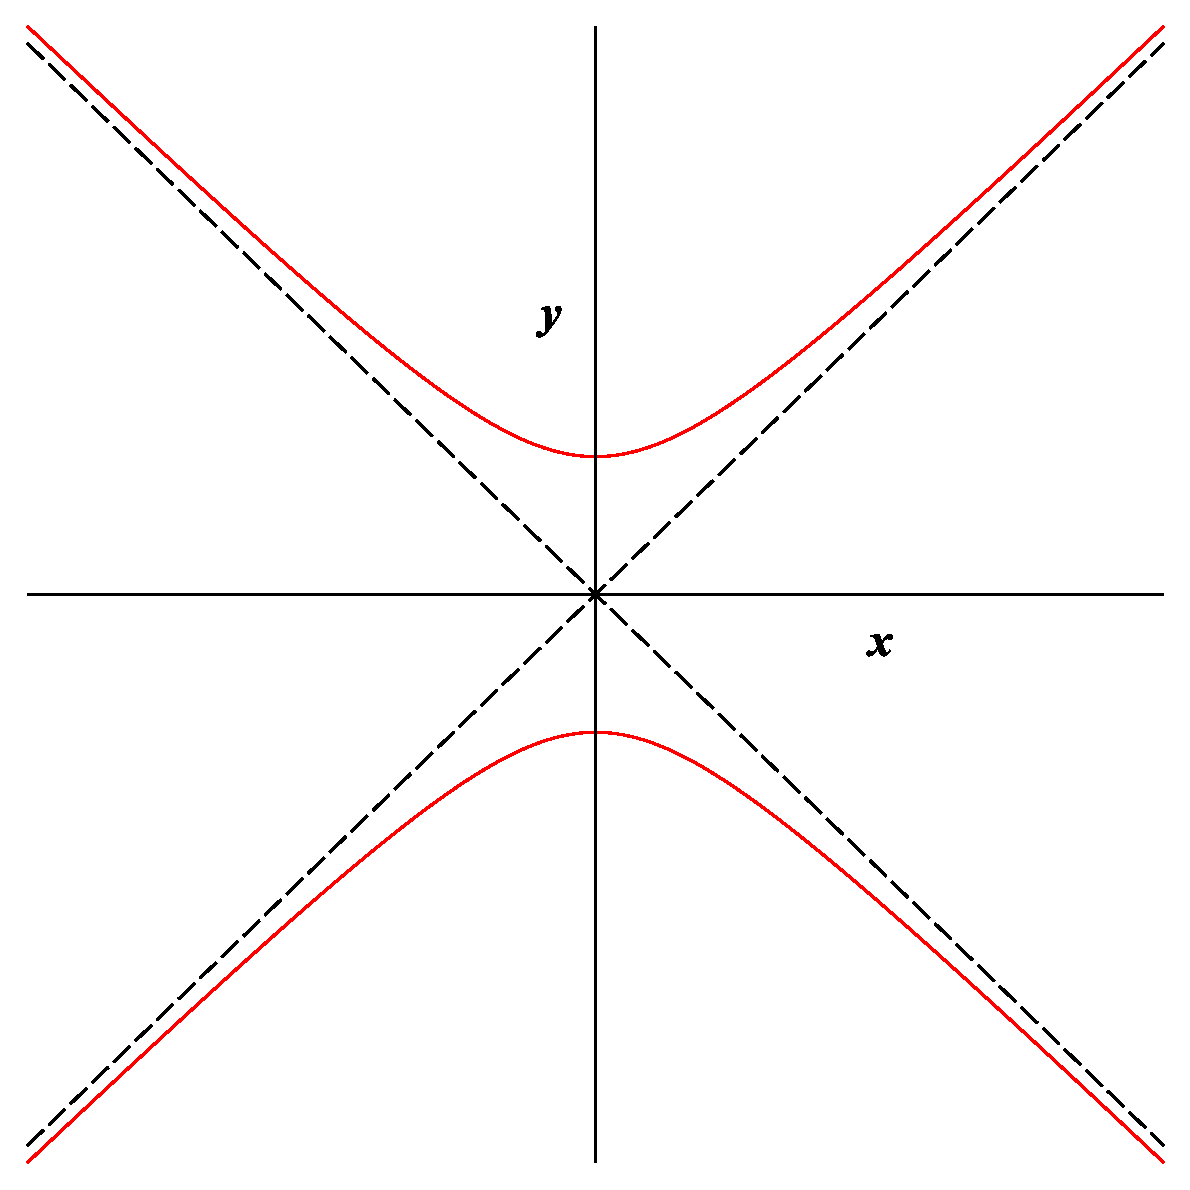
\includegraphics[keepaspectratio,width=8cm]{img/fig_8_9.eps}
		\end{figure}

		\newpage
		\item $\frac{x^2}{a^2} - \frac{y^2}{b^2} = 0 \Leftrightarrow \frac{x^2}{y^2} = \frac{a^2}{b^2} \Leftrightarrow y = \pm \frac{b}{a}x$. (Geradenpaar wie in obiger Skizze)
		\item $\frac{x^2}{a^2} - \frac{y^2}{b^2} - 1 = 0 \Leftrightarrow \frac{y^2}{b^2} - \frac{x^2}{a^2} + 1 = 0$ (analog zu (iv) mit Rolle von $x,y$ vertauscht)
		\item $\frac{x^2}{a^2} + y = 0 \Leftrightarrow y = - \frac{x^2}{a^2}$ (nach unten geöffnete Parabel)
		\item $\frac{x^2}{a^2} - y = 0 \Leftrightarrow y = \frac{x^2}{a^2}$ (nach oben geöffnete Parabel)
		\item $\frac{x^2}{a^2} + 1 = 0$ (leere Menge)
		\item $\frac{x^2}{a^2} = 0$ ($y$-Achse)
		\item $\frac{x^2}{a^2} - 1 = 0 \Leftrightarrow x = \pm a$ (Geradenpaar)
	\end{enumerate}
\end{beispiel}

\begin{beispiel}[Kegelschnitte, $n = 3$]
	\label{bsp:8.10}
	Eine klassische Motivation zum Studium der Quadriken kommt aus dem Studium der Kegelschnitte im $\RR^3$:
	Sei $K = \{(x,y,z) \in \RR^3 : x^2 + y^2 = z^2 \}$ der Kegelrand des \enquote{normierten} Kegels im $\RR^3$.
	Wir wollen die Schnitte von $K$ mit den zweidimensionalen Ebenen im $\RR^3$ untersuchen.
	Welche Gebilde können hier entstehen?
	\newpage
	
	\begin{figure}[h]
		\centering
		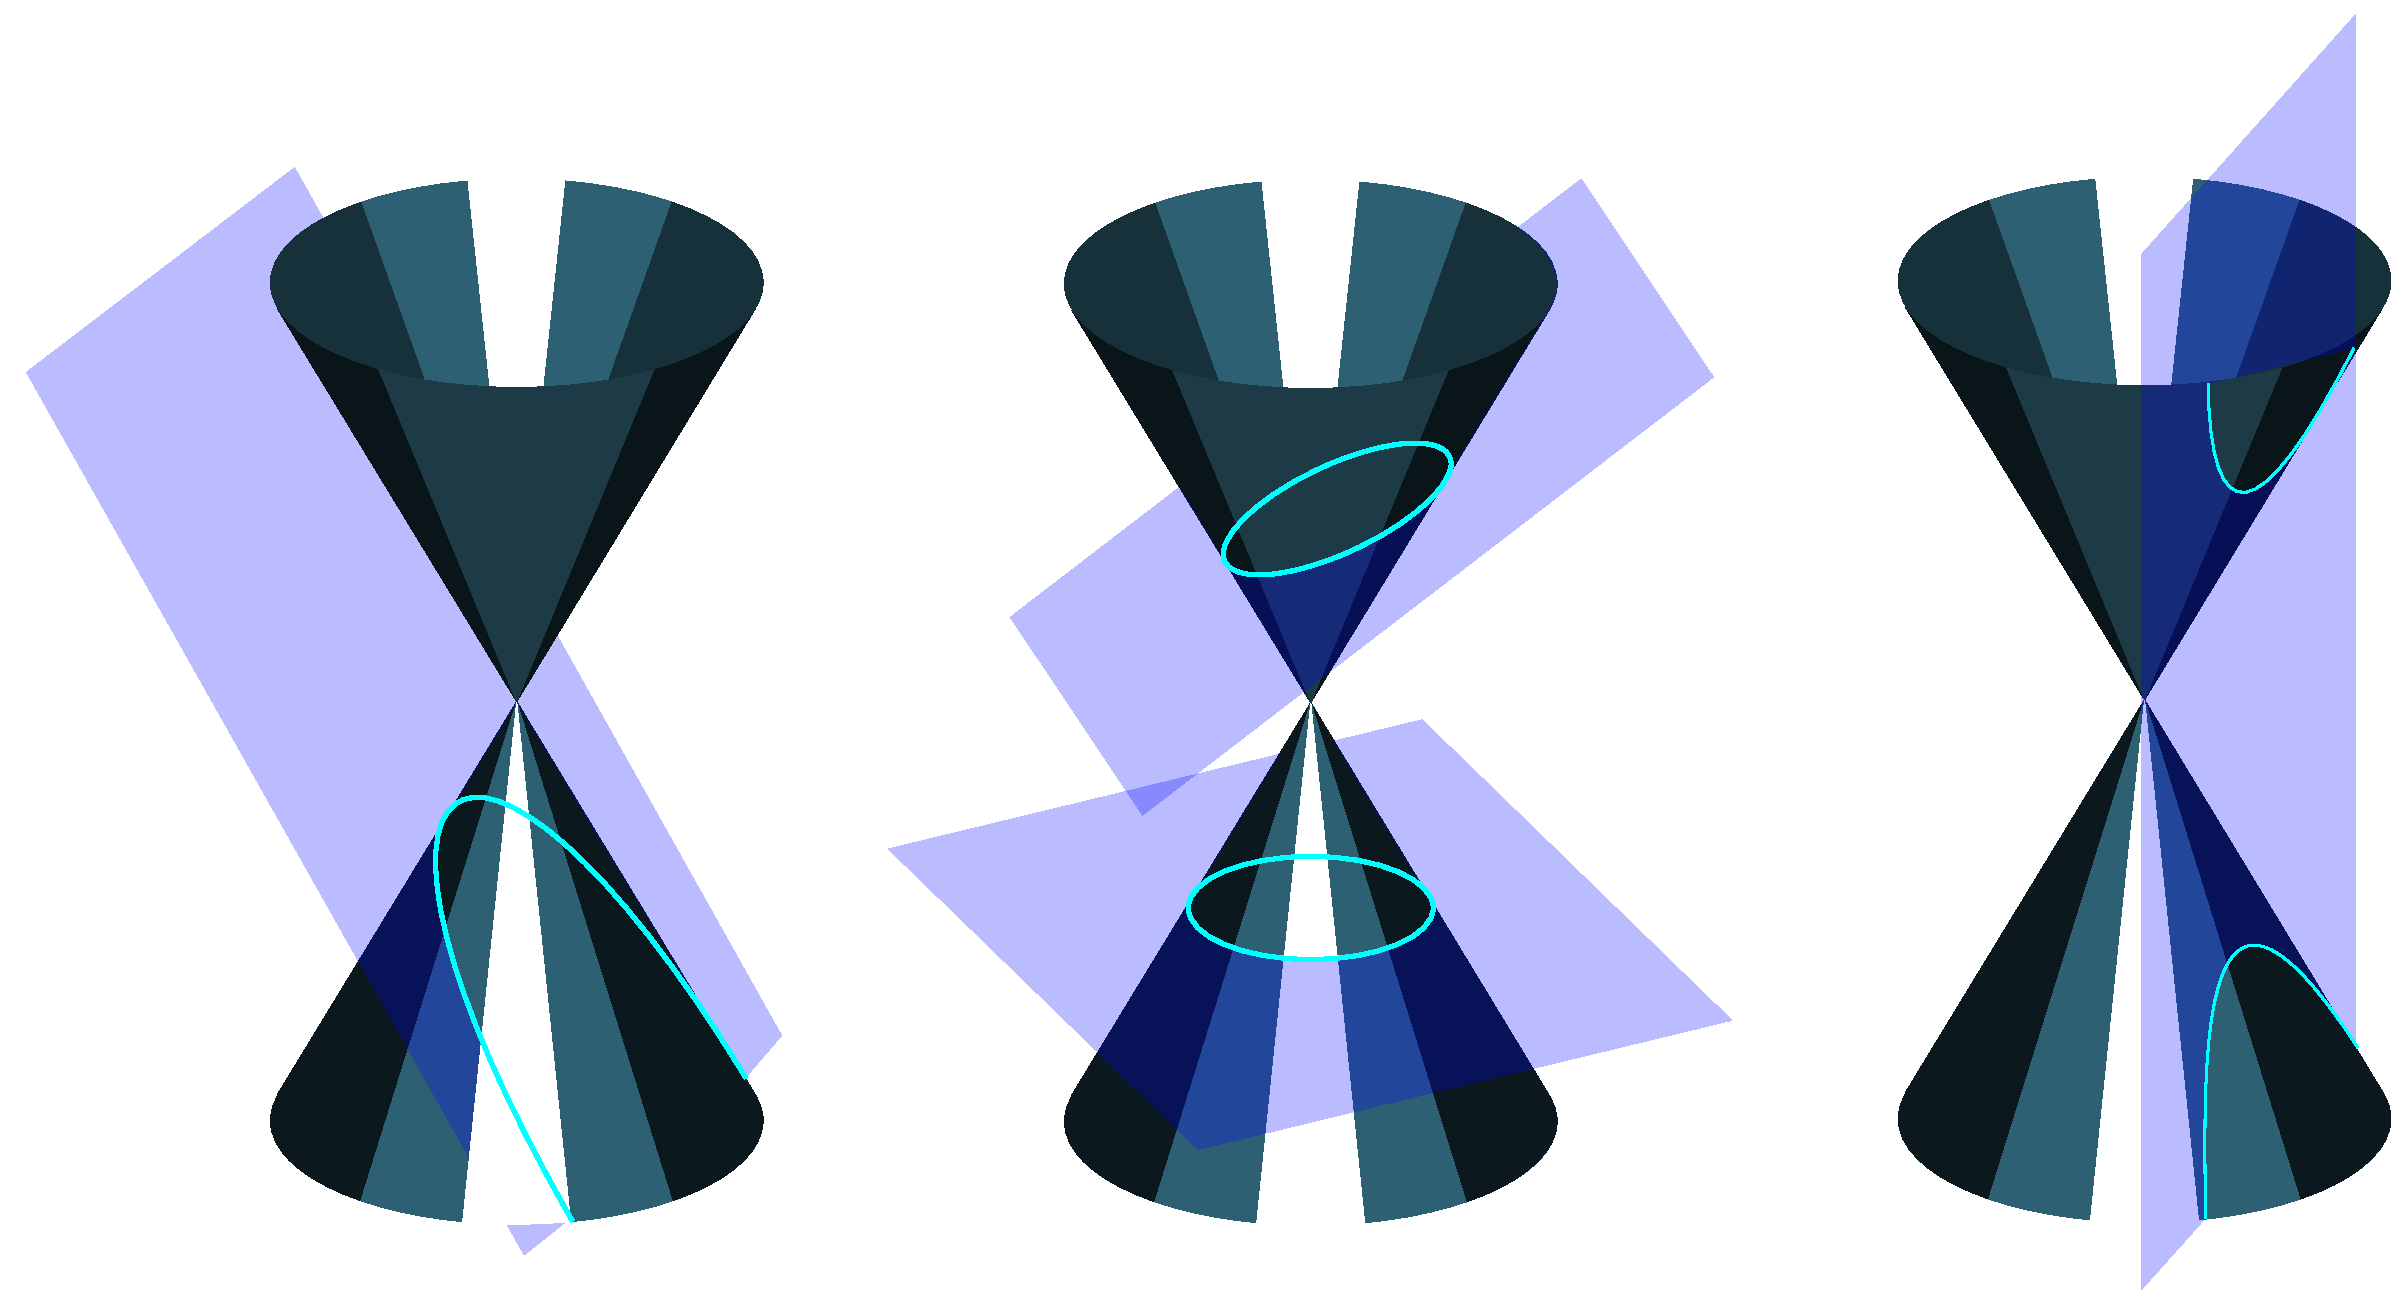
\includegraphics[keepaspectratio,width=10cm]{img/conic_sections.pdf}
		\caption{Die drei Arten von Kegelschnitten, die entstehen, wenn $K$ mit einer Ebene geschnitten wird. \cite{conic}}
	\end{figure}
	
	Eine Ebene im $\RR^3$ wird durch eine Gleichung der Form $ax + by + cz = d$ mit geeigneten Koeffizienten $a,b,c,d \in \RR$ beschrieben, wobei mindestens einer der Koeffizienten $a,b,c \neq 0$ sein muss.
	Ist $c \neq 0$, so folgt $z = \frac{1}{c} (d-ax-by)$.
	Einsetzen in die Kegelgleichung liefert
	\[
		x^2 + y^2 = \frac{1}{c^2} (d-ax-by)^2 = \frac{1}{c^2}(d^2 + a^2x^2 + b^2y^2 + 2abxy - dax - dby),
	\]
	also
	\begin{align*}
		0 &= \enb{\frac{a^2}{c^2}-1}x^2 + \enb{\frac{b^2}{c^2}-1}y^2 + \frac{2ab}{c^2} xy - \frac{2da}{c^2}x - \frac{2db}{c^2}y \\
		\Leftrightarrow \quad 0 &=(a^2-c^2)x^2 + (b^2-c^2)y^2 + 2abxy - 2dax - 2dby.
	\end{align*}
	Durch Wahl geeigneter Parameter bekommt man so alle Typen von Quadriken außer $\emptyset$ oder parallele Geradenpaare bzw. die $y$-Achse als Projektion von $K \cap E$ auf die $x$-$y$-Ebene.
\end{beispiel}

\newpage

%!TEX root = ../LA2.tex
\section{Die Jordan-Normalform}
\label{sec:2.9}

In diesem Abschnitt wollen wir Endomorphismen untersuchen, die nicht unbedingt diagonalisierbar sind.
Wir werden sehen, dass in vielen Fällen eine etwas schwächere Normalform der Darstellungsmatrix von $F$ möglich ist, die zum Beispiel immer noch ermöglicht, den Endomorphismus $\exp(F)$ für $F \in \End_{\CC}(V)$ bzw. $\exp(A)$ für $A \in M(n \times n, \CC)$ zu berechnen.
Wir werden diese Normalform dann später benutzen, um Differentialgleichungen zu lösen.
Wir starten mit:

\begin{definition}[trigonalisierbar]
	\mbox{} \\[-1.4cm]
	\label{def:9.1}
	\begin{enumerate}[(i)]
		\item Sei $V$ ein endlich dimensionaler $K$-Vektorraum und sei $F \in \End_K(V)$.
		Dann heißt $F$ \Index{trigonalisierbar}, falls eine Basis $B = \{v_1,\dots,v_n\}$ von $V$ existiert, sodass die Darstellungsmatrix $A_F^B$ von $F$ bezüglich $B$ eine obere Dreiecksmatrix ist, das heißt für geeignete $\lambda_1,\dots,\lambda_n \in K$ gilt
		\[
			A_F^B = \begin{pmatrix}
			\lambda_1 & * & \cdots & * \\ 
			0 & \lambda_2 & \cdots & * \\ 
			\vdots &  & \ddots & \vdots \\ 
			0 & \cdots & 0 & \lambda_n
			\end{pmatrix}. 
		\]
		\item Ist $A \in M(n \times n, K)$, so heißt $A$ \Index{trigonalisierbar}, falls ein $S \in \GL(n,K)$ existiert, sodass $S^{-1}AS$ eine obere Dreiecksmatrix ist.
	\end{enumerate}
\end{definition}

\begin{bemerkung}
	\mbox{} \\[-1.4cm]
	\label{bem:9.2}
	\begin{enumerate}[(i)]
		\item Ist $F \in \End_K(V)$ und $A \in M(n \times n,K)$ eine beliebige Darstellungsmatrix von $F$, so gilt:
		\[
			F \text{ ist trigonalisierbar} \quad \Leftrightarrow \quad A \text{ ist trigonalisierbar.}
		\]
		\item Ist $F$ (bzw. $A$) trigonalisierbar, so folgt für das charakteristische Polynom $\chi_F$ (und ähnlich für $\chi_A$), dass
		\[
			\chi_F(T) = \det(TE_n-A_F^B) = \det \begin{pmatrix}
			T-\lambda_1 & * & \cdots & * \\ 
			0 & T-\lambda_2 & \cdots & * \\ 
			\vdots &  & \ddots & \vdots \\ 
			0 & \cdots & 0 & T-\lambda_n
			\end{pmatrix} = \prod\limits_{i=1}^{n} (T-\lambda_i).
		\]
		Wir sehen also, dass $\chi_F$ in Linearfaktoren zerfällt und die Diagonalelemente $\lambda_i$ von $A^B_F$ sind gerade die Eigenwerte von $F$.
		\item Aus (ii) folgt:
		Die Matrix $A = \begin{pmatrix}
			0 & 1 \\ -1 & 0
		\end{pmatrix} \in M(2 \times 2,\RR)$ ist nicht trigonalisierbar, da $\chi_A(T) = T^2 +1$ über $\RR$ nicht in Linearfaktoren zerfällt.
		Fassen wir $A$ aber als komplexe Matrix auf, so ist $A$ sogar diagonalisierbar.
		Wir sehen, dass es für diese Fragen ganz wichtig ist, über welchem Körper $K$ wir arbeiten!
	\end{enumerate}
\end{bemerkung}
\newpage
Die Beobachtung in (ii) besitzt auch eine Umkehrung:

\begin{satz}
	\label{satz:9.3}
	Sei $V$ ein endlich dimensionaler $K$-Vektorraum und sei $F \in \End_K(V)$.
	Dann sind äquivalent:
	\begin{enumerate}[(i)]
		\item	$F$ ist diagonalisierbar.
		\item Das charakteristische Polynom $\chi_F$ von $F$ zerfällt in Linearfaktoren.
	\end{enumerate}
\end{satz}

\begin{bemerkung}
	\label{bem:9.4}
	Nach dem Fundamentalsatz der Algebra (\autoref{satz:1.11}) zerfällt jedes komplexe Polynom in Linearfaktoren.
	Aus \autoref{satz:9.3} folgt also insbesondere, dass jedes $F \in \End_{\CC}(V)$ trigonalisierbar ist, wenn $V$ ein endlich dimensionaler $\CC$-Vektorraum ist.
	Allgemeiner gilt:
	Ist $K$ ein \textbf{algebraisch abgeschlossener} Körper (das heißt, dass jedes Polynom über $K$ in Linearfaktoren zerfällt), und ist $V$ ein endlich dimensionaler $K$-Vektorraum, so ist jedes $F \in \End_K(V)$ trigonalisierbar. \index{algebraisch abgeschlossen}
\end{bemerkung}

Die Richtung (i) $\Rightarrow$ (ii) des Satzes folgt aus \autoref{bem:9.2}(ii).
Die andere Richtung werden wir in \autoref{satz:9.6} beweisen, wobei wir auch zeigen werden, dass die gesuche obere Dreiecksmatrix in einer besonderen Form gewählt werden kann.
Wir starten mit:

\begin{definition}[Jordan-Normalform]
	\mbox{} \\[-1.4cm]
	\label{def:9.5}
	\begin{enumerate}[(i)]
		\item Eine Matrix $J \in M(m \times m, K)$ heißt \Index{Jordan-Kasten}, falls ein $\lambda \in K$ existiert mit
		\[
			J = \begin{pmatrix}
			\lambda & 1 & 0 & \cdots & 0 \\ 
			0 & \lambda & 1 & \cdots & 0 \\ 
			\vdots &  & \ddots & \ddots & \vdots \\ 
			0 & \cdots & 0 & \lambda & 1 \\ 
			0 & \cdots & \cdots & 0 & \lambda
			\end{pmatrix}.
		\]
		Wir sagen dann auch, dass $J$ ein $\lambda$-Jordan-Kasten der Länge $m$ ist.
		\item Eine Matrix $A \in M(n \times n,K)$ heißt \textbf{in Jordan-Normalform} (oder einfach nur \Index{Jordan-Matrix}), falls \index{Jordan-Normalform}
		\[
			A = \begin{pmatrix}
			J_1 & 0 & \cdots & 0 \\ 
			0 & J_2 & \cdots & 0 \\ 
			\vdots &  & \ddots & \vdots \\ 
			0 & \cdots & 0 & J_r
			\end{pmatrix}, \text{ sodass }
			J_i = \begin{pmatrix}
			\lambda_i & 1 & 0 & \cdots & 0 \\ 
			0 & \lambda_i & 1 & \cdots & 0 \\ 
			\vdots &  & \ddots & \ddots & \vdots \\ 
			0 & \cdots & 0 & \lambda_i & 1 \\ 
			0 & \cdots & \cdots & 0 & \lambda_i
			\end{pmatrix} \in M(k_i \times k_i,K)
		\]
		für alle $1 \leq i \leq r$ ein Jordan-Kasten ist.
	\end{enumerate}
\end{definition}

Beachte:
\begin{enumerate}[(i)]
	\item Jede $1 \times 1$-Matrix ist ein Jordan-Kasten der Länge $1$, und damit ist auch jede Diagonalmatrix eine Jordan-Matrix.
	\item Die Eigenwerte $\lambda_i$ der Jordan-Kästen $J_i$ von $A$ müssen nicht paarweise verschieden sein!
	Ein konkretes Beispiel für eine Jordan-Matrix ist gegeben durch
	\[ 
	a = \enb{\begin{BMAT}(b){cccccccc}{cccccccc}
	2 & 1 & 0 & 0 & 0 & 0 & 0 & 0 \\ 
	0 & 2 & 1 & 0 & 0 & 0 & 0 & 0 \\ 
	0 & 0 & 2 & 0 & 0 & 0 & 0 & 0 \\ 
	0 & 0 & 0 & 2 & 1 & 0 & 0 & 0 \\ 
	0 & 0 & 0 & 0 & 2 & 0 & 0 & 0 \\ 
	0 & 0 & 0 & 0 & 0 & 3 & 0 & 0 \\ 
	0 & 0 & 0 & 0 & 0 & 0 & 3 & 1 \\ 
	0 & 0 & 0 & 0 & 0 & 0 & 0 & 3 
	\addpath{(0,8,|)rrrdddllluuu}
	\addpath{(3,5,|)rrddlluu}
	\addpath{(5,3,|)rdlu}
	\addpath{(6,2,|)rrddlluu}
	\end{BMAT}} = \begin{pmatrix}
		J_1 & 0 & 0 & 0 \\
		0 & J_2 & 0 & 0 \\
		0 & 0 & J_3 & 0 \\
		0 & 0 & 0 & J_4
	\end{pmatrix}
	\]
	mit den Jordan-Kästen
	\[
		J_1 = \begin{pmatrix}
			2 & 1 & 0 \\
			0 & 2 & 1 \\
			0 & 0 & 2
		\end{pmatrix}, J_2 = \begin{pmatrix}
			2 & 1 \\
			0 & 2
		\end{pmatrix}, J_3 = \begin{pmatrix}
		 3
		\end{pmatrix}, J_4 = \begin{pmatrix}
			3 & 1 \\
			0 & 3
		\end{pmatrix}.
	\]
\end{enumerate}

Im Rest dieses Abschnitts werden wir den folgenden Satz beweisen.
Als direkte Folgerung erhalten wir dann auch einen Beweis von \autoref{satz:9.3}.

\begin{satz}[Jordan-Normalform]
	\label{satz:9.6}
	Sei $V$ ein endlich dimensionaler $K$-Vektorraum und sei $F \in \End_K(V)$ so, dass das charakteristische Polynom $\chi_F$ von $F$ in Linearfaktoren zerfällt.
	Dann existiert eine Basis $B = \{v_1,\dots,v_n\}$ von $V$, sodass $A_F^B$ eine Jordan-Matrix ist.
	
	Analog: Ist $A \in M(n \times n, K)$ so, dass $\chi_A$ in Linearfaktoren zerfällt, dann existiert ein $S \in \GL(n,K)$, sodass $S^{-1}AS$ eine Jordan-Matrix ist.
\end{satz}

Wie üblich folgt der zweite Teil des Satzes direkt aus dem ersten Teil, wenn wir den Endomorphismus $F_A \colon K^n \rightarrow K^n, x \mapsto Ax$ betrachten und die Elemente der Basis $B$ von $K^n$ wie im ersten Teil des Satzes als Spalten der Matrix $S$ nehmen.

Für den Beweis des Satzes benötigen wir einige Vorbereitungen.

\begin{lemma}[Direkte Summen von Endomorphismen und Blockmatrizen]
	\label{def:9.7}
	Sei $V$ ein endlich dimensionaler $K$-Vektorraum und sei $F \in \End_K(V)$.
	Ist $V_1 \subseteq V$ mit $F(V_1) = V_1$, so können wir einen Endomorphismus $F_1 \in \End_K(V_1)$ durch $F_1(v) := F(v)$ für $v \in V_1$ definieren (also $F_1 = F \big|_{V_1} \colon V_1 \rightarrow V_1$).
	Besitzt $V$ eine direkte Summenzerlegung $V = V_1 \oplus V_2$ mit $F(V_1) \subseteq V_1$ und $F(V_2) \subseteq V_2$, so erhalten wir zwei Endomorphismen $F_1 \in \End_K(V_1)$ und $F_2 \in \End_K(V_2)$, und für jedes $v = v_1 + v_2 \in V$ mit $v_1 \in V_1, v_2 \in V_2$ gilt dann
	\[
		F(v) = F_1(v_1) + F_2(v_2).
	\]
	Wir sagen dann: $F$ ist die \Index{direkte Summe} von $F_1$ und $F_2$ und wir schreiben $F = F_1 \oplus F_2$.
	Sei nun $B_1 = \{v_1,\dots,v_r\}$ eine Basis von $V_1$ und $B_2 = \{v_{r+1},\dots,v_n\}$ eine Basis von $V_2$.
	Dann ist \linebreak $B := \{v_1,\dots,v_r,v_{r+1},\dots,v_n\}$ eine Basis von $V$ und für jedes $v_j$ aus dieser Basis gilt
	\[
	F(v_j) = \begin{cases}
	F_1(v_j) = \sum_{i=1}^{r} a_{ij} v_i, & \text{ falls } j \leq r \\
	F_2(v_j) = \sum_{i=r+1}^{n} a_{ij} v_i, & \text{ falls } r < j.
	\end{cases}
	\]
	Dann hat die Darstellungsmatrix $A := A_F^B$ von $F$ die Gestalt
	\[
	A = \begin{pmatrix}
	A_1 & 0 \\
	0 & A_2
	\end{pmatrix}, \text{ mit } A_1 = A_{F_1}^{B_1} \text{ und } A_2 = A_{F_2}^{B_2}.
	\]
	Sei umgekehrt $F$ ein beliebiger Endomorphismus von $V$, sodass eine Basis $B = \{v_1,\dots, v_r,v_{r+1},\dots,v_n\}$ von $V$ existiert mit $A_F^B = \begin{pmatrix}
	A_1 & 0 \\
	0 & A_2
	\end{pmatrix}$.
	Setzen wir dann $V_1 := \LH\{v_1,\dots,v_r\}$ und $V_2 := \{v_{r+1},\dots,v_n\}$, so folgt $V = V_1 \oplus V_2$ mit $F(V_i) \subseteq V_i$, also $F = F_1 \oplus F_2$ mit $F_i := F\big|_{V_i} \colon V_i \rightarrow V_i$ wie oben.
\end{lemma}

Wir benötigen:

\begin{lemma}
	\label{lemma:9.8}
	\mbox{} \\[-1.4cm]
	\begin{enumerate}[(i)]
		\item Sei $A = \begin{pmatrix}
		A_1 & * \\
		0 & A_2
		\end{pmatrix} \in M(n \times n, K)$ eine Blockmatrix.
		Dann gelten
		\[
			\det(A) = \det(A_1) \cdot \det(A_2) \quad \text{ und } \quad \chi_A = \chi_{A_1} \cdot \chi_{A_2},
		\]
		wobei $\chi_A, \chi_{A_1}$ und $\chi_{A_2}$ die charakteristischen Polynome von $A$, $A_1$ und $A_2$ bezeichnen.
		\item Sei $F = F_1 \oplus F_2$ die direkte Summe zweier Endomorphismen $F_i \in \End_K(V_i), i=1,2$.
		Dann gilt $\det(F) = \det(F_1) \cdot \det(F_2)$ und $\chi_F = \chi_{F_1} \cdot \chi_{F_2}$.
	\end{enumerate}
\end{lemma}

\begin{beweis}
	Sei $A_1 \in M(l \times l,K)$.
	Wir beweisen die Determinantenformel durch Induktion nach $l$.
	Für $l = 1$ folgt die Formel sofort durch Entwicklung der Determinante nach der ersten Spalte.
	Für den Induktionsschritt von $l-1$ nach $l$ sei $A = \begin{pmatrix}
		A_1 & * \\ 0 & A_2
	\end{pmatrix}$ mit $A_1 \in M(l \times l, K), l > 1$.
	Wir nehmen an, dass die Determinantenformel für Blöcke kleinerer Größe bereits bewiesen ist.
	Sei dann $A_i$ die Matrix, die durch Streichen der ersten Spalte und der $i$-ten Zeile von $A$ entsteht, und sei $A_{1,i}$ die Matrix, die durch Streichen der ersten Spalte und der $i$-ten Zeile von $A_1$ entsteht für $1 \leq i \leq l$.
	Dann gilt  $A_i = \begin{pmatrix}
		A_{1,i} & * \\
		0 & A_2
	\end{pmatrix}$ für alle $1 \leq i \leq r$.
	Da alle Einträge der ersten Spalte von $A$ unterhalb der $l$-ten Zeile verschwinden, erhalten wir durch Entwicklung der Determinante von $A$ (bzw. $A_1$) nach der ersten Spalte:
	\begin{align*}
		\det(A) &\stack{}{=} (-1)^{i+1} a_{i1} \det(A_i) = \sum_{i=1}^{l} (-1)^{i+1} a_{i1} \det \begin{pmatrix}
			A_{1,i} & * \\ 0 & A_2
		\end{pmatrix} \\
		&\stack{\text{I.A.}}{=} \sum_{i=1}^{l} (-1)^{i+1} a_{i1} \det(A_{1,i}) \det(A_2) = \det(A_1) \cdot \det(A_2).
	\end{align*}
	Die Formel für das charakteristische Polynom von $A$ folgt dann durch Anwenden der Determinantenformel auf $TE_n - A = \begin{pmatrix}
		T \cdot E_{n_1} - A_1 & * \\ 0 & T \cdot E_{n_2} - A_2
	\end{pmatrix}$, wobei $A_i \in M(n_i \times n_i,K), i=1,2$.
	Der Beweis von (ii) folgt nun aus (i) und der Tatsache, dass für $F = F_1 \oplus F_2$ eine Darstellungsmatrix der Gestalt $A_F^B = \begin{pmatrix}
		A_{F_1}^{B_1} & 0 \\ 0 & A_{F_2}^{B_2}
	\end{pmatrix}$ existiert. \qedhere
\end{beweis}

Völlig analog zum oben betrachteten Fall $F = F_1 \oplus F_2$ kann man auch direkte Summen von mehr als zwei Endomorphismen betrachten.
Sei dazu $V = V_1 \oplus V_2 \oplus \cdots \oplus V_r$ mit $F(V_i) \subseteq V_i$ für $1 \leq i \leq r$.
Ist $F_i \in \End_K(V_i)$ definiert durch $F_i = F\big|_{V_i}\colon V_i \rightarrow V_i$, so schreiben wir $F = F_1 \oplus F_2 \oplus \cdots \oplus F_r$ und sagen, dass $F$ die direkte Summe von $F_1,\dots,F_r$ ist.
Ist $B_i$ eine Basis von $V_i$ und $B = B_1 \cup \dots \cup B_r$, so folgt wie für den oben behandelten Fall $r=2$:
\[
	A_F^B = \begin{pmatrix}
		A_{F_1}^{B_1} & 0 & \cdots & 0 \\
		0 & \ddots & & \vdots \\
		\vdots & & \ddots & 0 \\
		0 & \cdots & 0 & A_{F_r}^{B_r}
	\end{pmatrix}.
\]
Mit \autoref{lemma:9.8} und einer leichten Induktion erhält man dann
\begin{equation}
	\det(F_1 \oplus \cdots \oplus F_r) = \prod_{i=1}^{r} \det(F_i) \quad \text{und} \quad \chi_F = \prod_{i=1}^{r} \chi_{F_r}. \label{eq:9.1}
\end{equation}

Zurück zur Jordan-Normalform.
Wir wollen zunächst untersuchen, wann $F \in \End_K(V)$ eine Basis $B$ besitzt, sodass $A_F^B$ aus genau einem Jordan-Kasten besteht:

\begin{lemma}
	\label{lemma:9.9}
	Sei $V$ ein endlich dimensionaler $K$-Vektorraum, $F \in \End_K(V)$ und sei $B = \{v_1,\dots,v_k\}$ eine Basis von $V$.
	Dann gilt
	\begin{equation}
		A_F^B = \begin{pmatrix}
		\lambda & 1 & 0 & \cdots & 0 \\ 
		0 & \lambda & 1 & \cdots & 0 \\ 
		\vdots &  & \ddots & \ddots & \vdots \\ 
		0 & \cdots & 0 & \lambda & 1 \\ 
		0 & \cdots & \cdots & 0 & \lambda
		\end{pmatrix} \quad \Leftrightarrow \quad (F-\lambda \id)(v_i) = \begin{cases}
			v_{i-1}, & \text{ falls } i > 1 \\
			0, & \text{ falls } i = 1
		\end{cases} \label{eq:9.2}
	\end{equation}
\end{lemma}

\begin{beweis}
	Wegen $A_{F - \lambda \id}^B = A_F^B - \lambda E_k$ ist die linke Aussage äquivalent zu $A_{F - \lambda \id}^B = \begin{pmatrix}
		0 & 1 & 0 & \cdots & 0 \\ 
		0 & 0 & 1 & \cdots & 0 \\ 
		\vdots &  & \ddots & \ddots & \vdots \\ 
		0 & \cdots & 0 & 0 & 1 \\ 
		0 & \cdots & \cdots & 0 & 0
		\end{pmatrix}$.
	Nach Definition einer Darstellungsmatrix ist dies aber äquivalent zur rechten Aussage.  \qedhere
\end{beweis}

\begin{bemerkung}
	\label{bem:9.10}
	Ist $F$ wie in \autoref{lemma:9.9} und ist $1 \leq l \leq k$, so gilt
	\[
		\Kern(F-\lambda \id)^l = \LH\{v_1,\dots,v_l\}.
	\]
	Insbesondere folgt $\Kern(F- \lambda \id)^k = \LH\{v_1,\dots,v_k\} = V$, also $(F-\lambda \id)^k = 0$.
	
	Allgemeiner gilt: Ist
	\[
		A:= A_F^B = \begin{pmatrix}
		J_1 & 0 & \cdots & 0 \\ 
		0 & J_2 & \cdots & 0 \\ 
		\vdots &  & \ddots & \vdots \\ 
		0 & \cdots & 0 & J_r
		\end{pmatrix}, \text{ sodass }
		J_i = \begin{pmatrix}
		\lambda_i & 1 & 0 & \cdots & 0 \\ 
		0 & \lambda_i & 1 & \cdots & 0 \\ 
		\vdots &  & \ddots & \ddots & \vdots \\ 
		0 & \cdots & 0 & \lambda_i & 1 \\ 
		0 & \cdots & \cdots & 0 & \lambda_i
		\end{pmatrix} \in M(k_i \times k_i,K)
	\]
	für jedes $1 \leq i \leq r$ ein Jordan-Kasten zum einzigen Eigenwert $\lambda$ von $F$ ist, so folgt
	\[
		A- \lambda E_n = \begin{pmatrix}
		N_1 & 0 & \cdots & 0 \\ 
		0 & N_2 & \cdots & 0 \\ 
		\vdots &  & \ddots & \vdots \\ 
		0 & \cdots & 0 & N_r
		\end{pmatrix} \text{ mit }
		N_i = \begin{pmatrix}
		0 & 1 & 0 & \cdots & 0 \\ 
		0 & 0 & 1 & \cdots & 0 \\ 
		\vdots &  & \ddots & \ddots & \vdots \\ 
		0 & \cdots & 0 & 0 & 1 \\ 
		0 & \cdots & \cdots & 0 & 0
		\end{pmatrix} \in M(k_i \times k_i,K).
	\]
	Damit folgt für $k := \max{k_1,\dots,k_r}$:
	\[
		(A-\lambda E_n)^k = \begin{pmatrix}
		N_1^k & 0 & \cdots & 0 \\ 
		0 & N_2^k & \cdots & 0 \\ 
		\vdots &  & \ddots & \vdots \\ 
		0 & \cdots & 0 & N_r^k
		\end{pmatrix} = 0,
	\]
	also auch $(F-\lambda \id)^k = 0$.
	Endomorphismen mit einer solchen Eigenschaft verdienen einen eigenen Namen!
\end{bemerkung}

\begin{definition}[nilpotent]
	\label{def:9.11}
	Sei $V$ ein $K$-Vektorraum.
	Ein $G \in \End_K(V)$ heißt \Index{nilpotent}, falls ein $k \in \NN$ existiert mit $G^k = 0$.

	Analog: Eine Matrix $N \in M(n \times n,K)$ heißt nilpotent, falls ein $k \in \NN$ existiert mit $N^k = 0$.

	Ist dann $k \in \NN$ minimal mit $G^k = 0$ (bzw. $N^k = 0$), so heißt $k$ die \Index{Nilpotenzlänge} von $G$ (bzw. $N$).
\end{definition}

Die Idee im Beweis der Existenz einer Jordan-Normalform für $F \in \End_K(V)$ besteht nun darin, den Raum $V$ in eine direkte Summe
\[
	V = V_{\lambda_1} \oplus V_{\lambda_2} \oplus \cdots \oplus V_{\lambda_m}
\]
zu zerlegen, und entsprechend $F$ in eine direkte Summe $F = F_{\lambda_1} \oplus \cdots \oplus F_{\lambda_m}$ mit $F_{\lambda_i} := F\big|_{V_{\lambda_i}} \colon V_{\lambda_i} \rightarrow V_{\lambda_i}$, wobei $\lambda_1, \dots, \lambda_m$ die paarweise verschiedenen Eigenwerte von $F$ sind und alle $F_i - \lambda_i \id \in \End_K(V_{\lambda_i})$ nilpotent sind.
Gelingt es uns dann, geeignete Basen $B_i$ für $V_{\lambda_i}$ anzugeben, sodass $A_{F_i}^{B_i}$ aus lauter $\lambda_i$-Jordan-Kästen besteht, so wird $B = B_1 \cup \cdots \cup B_m$ zu einer Jordan-Basis von $V$, das heißt $A_F^B$ ist in Jordan-Normalform.
Wir benötigen:

\begin{lemma}
	\label{lemma:9.12}
	Sei $V$ ein endlich dimensionaler $K$-Vektorraum und sei $G \in \End_K(V)$.
	Für alle $l \in \NN_0$ setze $V_l := \Kern(G^l) \subseteq V$.
	Dann gilt $G(V_l) \subseteq V_{l-1} \subseteq V_l$ für alle $l \in \NN$ und es existiert genau ein $k \in \NN_0$ mit
	\[
		\{0\} = V_0 \subsetneq V_1 \subsetneq V_2 \subsetneq \cdots \subsetneq V_k = V_{k+1}
	\]
	und $V_{l+1} = V_l$ für alle $l \geq k$.
	Insbesondere folgt: $G$ ist genau dann nilpotent, wenn $V_k = V$.
\end{lemma}

\begin{beweis}
	Wegen $G^{l-1}(G(V_l)) = G^l(V_l) = \setzero$ folgt $G(V_l) \subseteq \Kern(G^{l-1}) = V_{l-1}$, und ist $v \in V_{l-1}$, so folgt $G^l(v) = G(G^{l-1}(v)) = G(0) = 0$, also $v \in V_l$.
	Es folgt
	\[
		\setzero = V_0 \subseteq V_1 \subseteq \cdots \subseteq V_l \subseteq V_{l+1} \cdots.
	\]
	Wäre $V_{l+1} \neq V_l$ für alle $l \in \NN$, so wäre $\dim(V) \geq \dim(V_l) \geq l$ für alle $l \in \NN$, also $\dim(V) = \infty$.
	Da aber nach Voraussetzung $\dim(V) < \infty$ gilt, existiert ein kleinstes $k \in \NN_0$ mit $V_{k+1} = V_k$, und dann folgt
	\[
		\setzero = V_0 \subsetneq V_1 \subsetneq V_2 \subsetneq \cdots \subsetneq V_k = V_{k+1}
	\]
	wie im Lemma.
	Für $l \geq k$ gilt dann $V_{l+1} = V_l$, denn wäre $v \in V_{l+1} \setminus V_l$, so wäre $0 = G^{l+1}(v) = G^{k+1}(G^{l-k}(v))$, aber $0 \neq G^l(v) = G^k(G^{l-k}(v))$, also $G^{l-k}(v) \in V_{k+1} \setminus V_k = \emptyset$.
	Dies ist unmöglich. \qedhere
\end{beweis}
\newpage
%!TEX root = ../LA2.tex
\section{Eine Anwendung der Jordan-Normalform in der Analysis}
\label{sec:2.10}

In der Analysis, insbesondere in der Theorie der linearen Differentialgleichungen, ist es wichtig, Matrizen in Potenzreihen einsetzen zu können.
Insbesondere ist es wichtig, die matrixwertige Funktion

\[
	t \mapsto \exp(tB) \in M(n \times n, \CC)
\]

für eine Matrix $B \in M(n \times n, \CC)$ berechnen zu können.
In der Analysis II werden Sie dies direkt benutzen.
Wir starten mit:

\begin{definition}
	\label{def:10.1}
	Sei $\sum_{k=0}^{\infty} A_k$ eine Reihe von Matrizen in $M(n \times n, \KK)$ mit $\KK = \RR$ oder $\KK= \CC$, das heißt $A_k \in M(n \times n,\KK)$ für alle $k \in \NN_0$.
	Sei
	\[
		S_n := \sum_{k=0}^{n} A_k \in M(n \times n, \KK)
	\]
	die $n$-te \Index{Partialsumme} der Reihe.
	Wir sagen dann, dass die Reihe $\sum_{k=0}^{\infty} A_k$ gegen eine Matrix $S \in M(n \times n, \KK)$ \textbf{konvergiert}, wenn $(S_n)_{i,j} \rightarrow S_{i,j}$ für alle $1 \leq i,j \leq n$ gilt, wobei $(S_n)_{i,j}$ bzw. $S_{i,j}$ den $i,j$-ten Eintrag von $S_n$ bzw. $S$ bezeichnet.
	Wir schreiben dann $S := \sum_{k=0}^{\infty} A_k$. \index{Reihe} \index{Konvergenz}
\end{definition}

Wir wollen im Folgenden auch das Konzept der absoluten Konvergenz auf den Fall von Matrizenreihen übertragen.
Dazu benötigen wir:

\begin{definition}[Operatornorm]
	\label{def:10.2}
	Sei $\KK^n$ versehen mit dem Standard-Skalarprodukt $\sk{\cdot,\cdot}$ und der zugehörigen Norm $\no{\cdot}_2$.
	Ist dann $A \in M(n \times n, \KK)$, so definieren wir die \Index{Operatornorm} $\opn{A}$ von $A$ durch
	\[
		\opn{A} := \sup \{ \no{Az}_2 : z \in \KK^n \text{ mit } \no{z}_2 \leq 1\}.
	\]
\end{definition}

Da die Abbildung $z \mapsto \no{Az}_2$ stetig auf der kompakten Menge $B_1 = \{z \in \CC^n : \no{z}_2 \leq 1\}$ ist, nimmt sie auf $B_1$ ihr Maximum an.
Die Abbildung $\opn{\cdot}$ ist daher wohldefiniert.

\begin{lemma}
	\label{lemma:10.3}
	Die Abbildung $\opn{\cdot} \colon M(n \times n,\KK) \rightarrow [0,\infty), A \mapsto \opn{A}$ ist eine Norm auf dem $\KK$-Vektorraum $M(n \times n,\KK)$.
	Ferner gelten:
	\begin{enumerate}[(i)]
		\item $\no{Az}_2 \leq \opn{A} \no{z}_2$ für alle $A \in M(n \times n,\KK), z \in \KK^n$,
		\item $\opn{AB} \leq \opn{A} \opn{B}$ für alle $A,B \in M(n \times n, \KK)$ und
		\item $\sqrt{\sum_{i=1}^k \abs{a_{ij}}^2} \leq \opn{A}$ für alle $A \in M(n \times n, \KK), 1 \leq i,j \leq n$.
		Insbesondere folgt $\abs{a_{ij}} \leq \no{A}$ für alle $1 \leq i,j \leq n$.
	\end{enumerate}
\end{lemma}
\newpage
\begin{beweis}
	Man rechnet leicht nach, dass $\no{\lambda A}_2 = \no{\lambda} \cdot \opn{A}$ und $\opn{A} = 0 \Rightarrow A = 0$ gelten.
	Für die Dreiecksungleichung seien $A,B \in M(n \times n,\KK)$.
	Da die Abbildung $z \mapsto \no{(A+B)z}_2$ auf der Einheitskugel $B_1 \subseteq \KK^n$ ihr Maximum annimmt, existiert ein $z_0 \in B_1$ mit $\opn{A+B} = \no{(A+B)z_0}_2$.
	Dann folgt
	\begin{align*}
		\opn{A+B} &= \no{(A+B)z_0}_2 = \no{Az_0 + Bz_0}_2 \leq \no{Az_0}_2 + \no{Bz_0}_2 \\
		&\leq \sup_{\no{z}_2 \leq 1} \no{Az}_2 + \sup_{\no{z}_2 \leq 1} \no{B_z}_2 = \opn{A} + \opn{B}.
	\end{align*}
	Damit ist gezeigt, dass $\opn{\cdot}$ eine Norm ist.
	Die Aussage in (i) folgt direkt aus der Definition von $\opn{A}$:
	Ist $z=0$, so ist auch $Az = 0$ und es folgt $0 = \no{A\cdot0}_2 = \opn{A} \no{0}_2$.
	Ist $z \neq 0$, so ist $\frac{1}{\no{z}_2}\cdot z \in B_1$ und es folgt
	\[
		\no{Az}_2 = \no{A \enb{\frac{1}{\no{z}_2} \cdot z}}_2 \no{z}_2 \leq \opn{A} \no{z}_2.
	\]
	Für den Beweis von (ii) sei $z \in B_1$ beliebig.
	Dann folgt mit (i):
	\[
		\no{ABz}_2 \stackrel{\text{(i)}}{\leq} \opn{A} \no{Bz}_2 \stackrel{\text{(i)}}{\leq} \opn{A} \opn{B} \no{z}_2 \stackrel{\no{z}_2 \leq 1}{\leq} \opn{A} \opn{B}.
	\]
	Dann folgt auch $\opn{AB} = \sup_{z \in B_1} \no{ABz}_2 \leq \opn{A} \opn{B}$.
	
	Für den Beweis von (iii) sei $j \in \{1,\dots,n\}$ fest und betrachte $z = e_j \in B_1$.
	Dann folgt
	\[
		\sum_{i=1}^{n} \abs{a_{ij}}^2 = \no{Ae_j}_2^2 \leq \opn{A}^2.
	\]
	Es folgt $\sqrt{\sum_{i=1}^n \abs{a_{ij}}^2} \leq \opn{A}$.
	Da $\abs{a_{ij}} \leq \sqrt{\sum_{i=1}^n \abs{a_{ij}}^2}$, folgt (iii).	\qedhere
\end{beweis}

\begin{definition}[absolute Konvergenz]
	\label{def:10.4}
	Eine Reihe von Matrizen $\sum_{k=0}^{\infty}$ heißt \textbf{absolut konvergent}, wenn $\sum_{k=0}^{\infty} \opn{A_k}$ in $\RR$ konvergiert. \index{absolute Konvergenz}
\end{definition}

\begin{bemerkung}
	\label{bem:10.5}
	Anstelle von $\opn{\cdot}$ könnte man hier auch jede andere Norm auf $M(n \times n, \KK)$ einsetzen.
	Da alle Normen auf endlich dimensionalen Räumen äquivalent sind, wäre der entsprechende Begriff von absoluter Konvergenz äquivalent zu dem obigen.
\end{bemerkung}

\begin{satz}
	\label{satz:10.6}
	Jede absolut konvergente Reihe $\sum_{k=0}^{\infty} A_k$ ist konvergent.
	Es gilt dann sogar, dass für jedes $1 \leq i,j \leq n$ die Reihe der $i,j$-ten Einträge $\sum_{k=0}^{\infty} (A_k)_{i,j}$ von $\sum_{k=0}^{\infty} A_k$ absolut konvergent ist.
\end{satz}

\begin{beweis}
	Nach \autoref{lemma:10.3} gilt für alle $1 \leq i,j \leq n$:
	\[
		\sum_{k=0}^{\infty} \abs{(A_k)_{i,j}} \leq \sum_{k=0}^{\infty} \opn{A_k}.
	\]
	Damit ist $\sum_{k=0}^{\infty} \opn{A_k}$ eine konvergente Majorante von $\sum_{k=0}^{\infty} \abs{(A_k)_{i,j}}$.	\qedhere
\end{beweis}

\begin{korollar}
	\label{kor:10.7}
	Sei $f(z) = \sum_{k=0}^{\infty} a_kz^k$ eine Potenzreihe in $\KK$ mit Konvergenzradius $R > 0$, das heißt die Reihe konvergiert für alle $z \in \KK$ mit $\abs{z} < R$ absolut und sie divergiert, wenn $\abs{z} > R$. \index{Konvergenzradius}
	Ist dann $A \in M(n \times n,\KK)$ mit $\opn{A} < R$, so konvergiert die Reihe $f(A) := \sum_{k=0}^{\infty} a_k A^k$ absolut in $M(n \times n,\KK)$.
\end{korollar}

\begin{beweis}
	Nach \autoref{lemma:10.3}(ii) gilt $\opn{A^k} \leq \opn{A}^k$ für alle $k \in \NN_0$.
	Damit folgt
	\[
		\sum_{k=0}^{\infty} \opn{a_k A^k} = \sum_{k=0}^{\infty} \abs{a_k} \opn{A^k} \leq \sum_{k=0}^{\infty} \abs{a_k} \opn{A}^k < \infty.
	\]
	Da $\opn{A} < R$, ist die Reihe auf der rechten Seite konvergent. \qedhere
\end{beweis}

Die Exponentialreihe $\exp(z) = \sum_{k=0}^{\infty} \frac{1}{k!} z^k$ hat bekanntlich den Konvergenzradius $R = \infty$.
Wenden wir die Folgerung auf diese Reihe an, so können wir definieren:

\begin{definition}[Exponentialfunktion für Matrizen]
	\label{def:10.8}
	Für $B \in M(n \times n,\CC)$ definieren wir
	\[
	\exp(B) := \sum\limits_{k=0}^\infty \frac{1}{k!} B^k,
	\]
	mit $B^0 := E$. \index{Exponentialfunktion}
\end{definition}

\begin{bemerkung}
	\label{bem:10.9}
	\mbox{} \\[-1.4cm]
	\begin{enumerate}[(i)]
		\item Ist $B \in M(n \times n,\RR)$ eine reelle Matrix, so ist nach (i) jede Komponente von $\exp(B)$ ein Grenzwert einer reellen Folge, und damit ist auch $\exp(B) \in M(n \times n,\RR)$.
		\item Ist $A = C^{-1} BC$ für ein $C \in \GL(n,\CC)$, so folgt
		\begin{align*}
		A^{k} &= (C^{-1}BC)\cdot (C^{-1}BC) \cdots (C^{-1}BC) \\
		&= C^{-1} B (CC^{-1}) B (CC^{-1}) \cdots (CC^{-1})BC \\
		&= C^{-1} B E B E \cdots E BC = C^{-1} B^k C
		\end{align*}
		für jedes $k \in \NN_0$, und damit folgt:
		\[
			\exp(A) = \sum\limits_{k=0}^{\infty} \frac{1}{k!} A^k = \sum_{k=0}^{\infty} \frac{1}{k!} C^{-1} B^{k} C \stackrel{(*)}{=} C^{-1} \enb{\sum_{k=0}^{\infty} \frac{1}{k!} B^{k}} C = C^{-1} \exp(B) C.
		\]
		Hierbei folgt die Gleichung $(*)$ wegen der Stetigkeit der Abbildung $A \mapsto C^{-1} AC$ bezüglich $\opn{\cdot}$, denn für alle $A,B \in M(n \times n,\CC)$ gilt
		\[
			\opn{C^{-1}AC - C^{-1}BC} = \opn{C^{-1}(A-B)C} \leq \opn{C^{-1}} \opn{C} \opn{A-B}.
		\]
	\end{enumerate}
\end{bemerkung}

Ähnlich wie im Komplexen erhält man eine überaus nützliche Funktionalgleichung:

\begin{lemma}
	\label{lemma:10.10}
	Seien $A,B \in M(n \times n,\CC)$ mit $AB = BA$.
	Dann gilt $\exp(A+B) = \exp(A) + \exp(B)$.
\end{lemma}

\begin{beweis}[Skizze]
	Sind $A,B \in M(n \times n,K)$ mit $AB = BA$, so folgt mit dem üblichen Induktionsbeweis die Binomische Formel \index{binomische Formel}
	\[
	(A+B)^{k} = \sum_{j=0}^{k} \binom{k}{j} A^{j} \cdot B^{k-j}
		\]
	für alle $k \in \NN_0$.
	Mit dem Cauchy-Produkt für absolut konvergente Reihen (in einer entsprechenden Version für Matrixreihen) folgt dann
	\begin{align*}
	\exp(A+B) &= \sum_{k=0}^{\infty} \frac{1}{k!} (A+B)^k = \sum_{k=0}^{\infty} \frac{1}{k!} \enb{\sum_{j=0}^{k} A^{j} B^{k-j}} \\
	&= \sum_{k=0}^{\infty} \enb{\sum_{j=0}^{k} \enb{\frac{1}{j!} A^{j}} \cdot \enb{\frac{1}{(k-j)!} B^{k-j}}} = \enb{\sum_{j=0}^{\infty} \frac{1}{j!} A^{j}} \cdot \enb{\sum_{k=0}^{\infty} \frac{1}{k!} B^{k}} \\
	&= \exp(A) \cdot \exp(B) \qedhere
	\end{align*}
\end{beweis}

\minisec{Systeme linearer Differentialgleichungen}
In vielen physikalischen Anwendungen ist es notwendig, System von \textbf{Differentialgleichungen} der Form \index{Differentialgleichung}
\begin{align*}
	y_1'(t) &= b_{11} \cdot y_1(t) + b_{12} \cdot y_2(t) + \cdots + b_{1n} \cdot y_n(t) + f_1 (t) \\
	y_2'(t) &= b_{21} \cdot y_1(t) + b_{22} \cdot y_2(t) + \cdots + b_{2n} \cdot y_n(t) + f_2 (t)\\
	& \qquad \qquad \qquad \vdots \\
	y_n'(t) &= b_{n1} \cdot y_1(t) + b_{n2} \cdot y_2(t) + \cdots + b_{nn} \cdot y_n(t) + f_n(t)
\end{align*}
zu betrachten, wobei $I \subseteq \RR$ ein Intervall, $y_1,\dots,y_n\colon I \rightarrow \RR$ differenzierbare reelle Funktionen, $b_{ij} \in \RR$ für alle $1 \leq i,j \leq n$ und $f_1,\dots,f_n \colon I \rightarrow \RR$ stetige Funktionen sind.
Ist dann $B = (b_{ij}) \in M(n \times n, \RR)$, so können wir das System auch in der Kurzschreibweise
\[
	y'(t) = B \cdot y(t) + f(t), \quad y(t) := (y_1(t),\dots,y_n(t))^T, \quad f(t) := (f_1(t),\dots,f_n(t))^T
\]
formulieren, wobei dann $y'(t) := (y_1'(t),\dots,y_n'(t))^T$ die komponentenweise Ableitung von $y\colon I \rightarrow \RR^n$ bezeichnet.
Definieren wir die Konvergenz von Vektoren durch die Konvergenz der Komponenten, so ist $y \colon \RR \rightarrow \RR^n$ differenzierbar in $t$ genau dann, wenn

\[
	y'(t) = \lim\limits_{h \rightarrow 0} \frac{1}{h} (y(t+h)-y(t))
\]

existiert.
In der Regel wird zusätzlich zum oben gegebenen System von Differentialgleichungen noch eine Anfangsbedingung
\[
	y(t_0) = y_0 = (y_{10},\dots,y_{n0})^T
\]
vorgegeben, wobei $t_0 \in I$ eine gegebene Anfangszeit ist.
Gesucht sind also alle komponentenweise differenzierbaren Funktionen $y \colon I \rightarrow \RR^n$ mit $y' = B \cdot y + f(t)$ und $y(t_0) = y_0$.
Eine Gleichung dieser Form heißt \textbf{System von linearen Differentialgleichungen erster Ordnung mit konstanten Koeffizienten} mit der Anfangsbedingung $y(t_0) = y_0$.
Ist $f \equiv 0$, so heißt $y' = By$ \textbf{homogenes System linearer Differentialgleichungen erster Ordnung}.

\begin{beispiel}
	\label{bsp:10.11}
	Ein Zahlen-Beispiel:
	Gesucht sind alle differenzierbaren Funktionen $y_1,y_2,y_3\colon \RR \rightarrow \RR$ mit
	\begin{align*}
	y_1'(t) &= y_1(t) + 2y_2(t) - y_3(t) + \sin(t) \\
	y_2'(t) &= -y_2(t) + y_3(t) - \cos(t) \\
	y_3'(t) &= 3y_1(t) + y_2(t) + t
	\end{align*}
	und der Anfangsbedingung $y_1(0) = 1, y_2(0) = 0, y_3(0)=2$.
	Ist dann $B = \begin{pmatrix}
		1 & 2  & -1 \\
		0 & -1 & 1  \\
		3 & 0  & 1
	\end{pmatrix}$, so ist das obige System von Differentialgleichungen gegeben durch die Gleichung $y' = By(t) + f(t)$, $y(0) = (1,0,2)^T$, wobei $y = (y_1,y_2,y_3)^T \colon \RR \rightarrow \RR^3$ die gesuchte $\RR^3$-wertige Funktion ist.
\end{beispiel}

\begin{bemerkung}
	\label{bem:10.12}
	\mbox{} \\[-1.4cm]
	\begin{enumerate}[(i)]
		\item Tatsächlich ist es nützlich, sich nicht auf den Fall reeller Funktionen zu beschränken, sondern auch komplexwertige Funktionen und komplexe Matrizen zuzulassen.
		Ist dabei $f\colon I \rightarrow \CC$, so ist $f$ differenzierbar in $t \in \RR$, wenn $f'(t) := \lim\limits_{h \rightarrow 0} \frac{f(t+h) - f(t)}{h}$ existiert.
		Ist $f = g + ih$ und $g,h \colon \RR \rightarrow \RR$, so ist $f$ genau dann differenzierbar in $t$, wenn $g$ und $h$ in $t$ differenzierbar sind, und dann gilt $f'(t) = g'(t) + ih'(t)$.
		Mit diesem Verständnis für die Differenzierbarkeit komplexwertiger Funktionen auf $\RR$ können wir jetzt auch Systeme der Form
		\[
			y' = By +f, \quad y(t_0)=y_0
		\]
		mit $B \in M(n \times n,\CC)$ und $y_0 \in \CC^n$ betrachten.
		Die gesuchte Lösung ist dann eine Funktion $y\colon I \rightarrow \CC^n$.
		Wir werden im Folgenden diesen allgemeineren Fall betrachten.
		\item Durch die Substitution $t \mapsto t-t_0$ können wir uns immer auf den Fall $t_0 = 0$ beschränken:
		Dazu setze $J := I-t_0 = \{t-t_0 : t \in I\}$ und $\wt{f} \colon J \rightarrow \CC^n, \wt{f}(t) := f(t+t_0)$.
		Ist $\wt{y} \colon J \rightarrow \CC^n$ mit $\wt{y}' = B \wt{y} + \wt{f}$ und $\wt{y}(0) = y_0$ und setzen wir $y(t) := \wt{y}(t-t_0)$, so folgt sofort aus den Ableitungsregeln, dass $y' = By + f$ mit $y(t_0) = y_0$.
	\end{enumerate}
\end{bemerkung}

Im eindimensionalen Fall ist es sehr leicht, eine Lösung der homogenen Differentialgleichung $y'(t) = b \cdot y(t), y(0) = y_0$ anzugeben.
Nachrechnen zeigt sofort, dass $y(t) = e^{tb} y_0$ eine Lösung dieser Gleichung ist.
Mit etwas mehr Mühe sieht man dann sogar ein, dass dies die einzige Lösung der Gleichung ist.
Wir werden gleich sehen, dass eine ähnliche Formel auch für Systeme gilt.

Ist $B \in M(n \times n,\CC)$, so wollen wir dafür die matrixwertige Funktion
\begin{align*}
	Y\colon \RR &\longrightarrow \CC^{n} \\
	t &\longmapsto \exp(tB)
\end{align*}
betrachten.
Wir definieren Differenzierbarkeit von matrixwertigen Funktionen wie für vektorwertige Funktionen durch die Differenzierbarkeit aller Komponenten.
Dies ist wieder äquivalent zur komponentenweisen Existenz des Grenzwertes
\[
	Y'(t) = \lim\limits_{h \rightarrow 0} \frac{1}{h}(Y(t+h)-Y(t)).
\]

\begin{satz}
	\label{satz:10.13}
	Seien $B \in M(n \times n,\CC)$, $Y(t) := \exp(tB)$ und $y_0 \in \CC^{n}$.
	Dann gelten:
	\begin{enumerate}[(i)]
		\item $Y'(t) = B \cdot \exp(tB) = B \cdot Y(t)$.
		\item $y\colon \RR \rightarrow \CC^{n}, y(t) := \exp(tB) \cdot y_0$ ist eine Lösung des Systems $y' = B \cdot y, y(0) = y_0$.
	\end{enumerate}
\end{satz}

\begin{beweis}
	Betrachten wir die Funktion $Y(t) = \exp(tB) = \sum_{k=0}^{\infty} \frac{1}{k!} t^{k} B^{k}$, so stellen wir fest, dass jede Komponente $Y(t)_{ij}$ von $Y(t)$ durch eine Potenzreihe $\sum_{k=0}^{\infty} d_{ij}(k)t^{k}$ gegeben ist, wobei $d_{ij}(k)$ die $i,j$-te Komponente der Matrix $\frac{1}{k!} B^{k}$ ist.
	Da die Exponentialreihe für alle $tB$ konvergiert, haben alle diese Reihen unendlichen Konvergenzradius, und wir dürfen auf ganz $\RR$ gliedweise differenzieren (siehe Analysis).
	Damit folgt:	
	\[
		Y'(t) = \sum_{k=1}^{\infty} \frac{1}{k!} kt^{k-1} B^{k} = B \cdot \enb{\sum_{k=1}^{\infty} \frac{1}{(k-1)!} t^{k-1} B^{k-1}} = B \cdot \enb{\sum_{k=0}^{\infty} \frac{1}{k!} t^{k} B^{k}} = B \cdot \exp(tB) = B \cdot Y(t).
	\]
	Mit (i) erhalten wir für $y(t) = Y(t) \cdot y_0$:
	\begin{align*}
		y'(t) &= \lim\limits_{h \rightarrow 0} \frac{1}{h} (y(t+h)-y(t)) = \lim\limits_{h \rightarrow 0} \frac{1}{h} (Y(t+h) \cdot y_0 - Y(t) \cdot y_0) \\
		&= \enb{\lim\limits_{h \rightarrow \infty} \frac{1}{h}(Y(t+h)-Y(t))} \cdot y_0 = B \cdot Y(t) \cdot y_0 = B \cdot y(t)
	\end{align*}
	und $y(0) = \exp(0\cdot B) \cdot y_0 = E \cdot y_0 = y_0$. \qedhere
\end{beweis}

\begin{bemerkung}
	\label{bem:10.14}
	\mbox{} \\[-1.4cm]
	\begin{enumerate}[(i)]
		\item Man kann auch hier zeigen, dass die im Satz angegebene Lösung die einzige Lösung des homogenen Anfangswertproblems $y' = By$ mit der Anfangsbedingung $y(0) = y_0$ ist.
		\item Da $\exp(tB) \in M(n \times n,\RR)$, wenn $B \in M(n \times n,\RR)$ (siehe \autoref{bem:10.9}), folgt:
		Sind $B$ und $y_0$ reell, so ist auch $y(t)$ für alle $t \in \RR$ reell.
	\end{enumerate}
\end{bemerkung}

Wir wollen nun noch eine Lösungsformel für das inhomogene Anfangswertproblem
\[
	y' = By + f, \quad y(0) = y_0
\]
angeben.
Hierfür betrachten wir den Ansatz $y(t) = Y(t)c(t)$ für eine stetig differenzierbare Funktion $c \colon I \rightarrow \CC^n$ und $Y(t) = \exp(tB)$.
Einsetzen liefert wegen $y(0) = Y(0)c(0) = c(0)$ und $Y'(t) = BY(t)$:
\begin{align*}
	Y'(t) c(t) + Y(t) c'(t) &= BY(t)c(t) + f(t) \\
	\Leftrightarrow \qquad Y(t) c'(t) &= f(t) \\
	\Leftrightarrow \qquad c'(t) &= Y(t)^{-1} f(t) \\
	\Leftrightarrow \qquad c(t) &= c(0) + \int_{0}^{t} Y(s)^{-1} f(x) ds \\
	\Leftrightarrow \qquad c(t) &= y_0 + \int_{0}^{t} \exp(-sB)f(s)ds,
\end{align*}
wobei wir im letzten Schritt benutzt haben, dass $\exp(-tB) \exp(tB) = \exp((-t+t)B) = \exp(0) = E_n$ gilt, also $Y(t)^{-1} = \exp(tB)^{-1} = \exp(-tB)$ für alle $t \in \RR$.
Zusammen erhalten wir nun:

\begin{satz}
	\label{satz:10.15}
	Sei $A \in M(n \times n, \CC)$ und $f \colon I \rightarrow \CC$ stetig mit $0 \in I$.
	Dann ist
	\[
		y(t) = \exp(tB) \enb{y_0 + \int_{0}^{t} \exp(-sB) f(s) ds}
	\]
	eine Lösung des Anfangswertproblems $y' = By + f, y(0) = y_0$.
\end{satz}

\begin{anwendung}[Berechnung der Funktion]
	\label{anw:10.16}
	Wir wollen nun überlegen, wie wir die Funktion $Y(t) = \exp(tB)$ für $B \in M(n \times n,\CC)$ mit Hilfe einer Jordan-Normalform von $B$ explizit berechnen können.
	Da jedes Polynom über $\CC$ in Linearfaktoren zerfällt, können wir nach \autoref{satz:9.6} eine Matrix $C \in \GL(n,\CC)$ finden (und im Prinzip auch berechnen), sodass $A = C^{-1}BC$ eine Jordan-Matrix ist.
	Dann folgt $tB = CtAC^{-1}$ und $\exp(tB) = C \exp(tA)C^{-1}$.
	Es genügt also zu wissen, wie die Funktion $\exp(tA)$ für jede Jordan-Matrix $A$ berechnet werden kann.
	
	Sei nun $A = \begin{pmatrix}
	J_1 &        &  \\
	& \ddots &  \\
	&        & J_m
	\end{pmatrix}$ eine beliebige Jordan-Matrix mit den Jordan-Kästen $J_1,\dots,J_m$.
	Nach den Rechenregeln für Blockmatrizen gilt dann
	\[
	A^{k} = \begin{pmatrix}
	J_1^{k} &        &  \\
	& \ddots &  \\
	&        & J_m^{k}
	\end{pmatrix} \quad \text{und} \quad \exp(tA) =
	\begin{pmatrix}
	\exp(tJ_1) &        &  \\
	& \ddots &  \\
	&        & \exp(tJ_m)
	\end{pmatrix}.
	\]
	Es genügt also zu wissen, wie die Matrix $\exp(tJ)$ zu berechnen ist, wenn $J$ ein Jordan-Kasten zum Eigenwert $\lambda$ ist.
	Dann gilt:
	
	\[
	J = \begin{pmatrix}
	\lambda & 1       & 0      & \cdots  & 0       \\
	0       & \lambda & 1      & \cdots  & 0       \\
	\vdots  &         & \ddots & \ddots  & \vdots  \\
	0       & \cdots  & 0      & \lambda & 1       \\
	0       & \cdots  & \cdots & 0       & \lambda
	\end{pmatrix} = \lambda E + N \text{ mit } N:=
	\begin{pmatrix}
	0      & 1      & 0      & \cdots & 0      \\
	0      & 0      & 1      & \cdots & 0      \\
	\vdots &        & \ddots & \ddots & \vdots \\
	0      & \cdots & 0      & 0      & 1      \\
	0      & \cdots & \cdots & 0      & 0
	\end{pmatrix}.
	\]
	Da $\lambda E \cdot N = N \cdot \lambda E$, folgt mit \autoref{lemma:10.10}, dass
	\[
	\exp(tJ) = \exp(t\lambda E + tN) = \exp(t \lambda E) \cdot \exp(tN).
	\]
	Wegen $(t\lambda E)^{k} = (t\lambda)^{k}E$ folgt
	\[
	\exp(t\lambda E) = \sum_{k=0}^{\infty} \frac{1}{k!} (t \lambda E)^{k} = \enb{\sum_{k=0}^{\infty} \frac{1}{k!} (t\lambda)^{k}} E = e^{t\lambda} E.
	\]
	Eine leichte Rechnung (benutze \autoref{lemma:9.9}) ergibt ferner, dass $N^{l} = (0, \dots, 0,e_1,\dots,e_{k-l})$, wobei die ersten $l$ Einträge aus Nullspalten bestehen und dann die ersten $k-l$ Einheitsvektoren des $\CC^{k}$ als weitere Spalten der Matrix $N^{l}$ auftreten.
	Insbesondere gilt $N^{k} = 0$.
	Einsetzen in die Exponentialreihe ergibt (mit $N^0 = E$):
	\[
	\exp(tN) =
	\begin{pmatrix}
	1 & t      & \frac{t^2}{2} & \frac{t^3}{3!} & \cdots         & \frac{t^{k-1}}{(k-1)!} & \frac{t^{k}}{k!}       \\
	0 & 1      & t             & \frac{t^2}{2}  & \frac{t^3}{3!} & \cdots                 & \frac{t^{k-1}}{(k-1)!} \\
	& \ddots & \ddots        & \ddots         &                &                        &  \\
	&        & \ddots        & \ddots         & \ddots         &                        &  \\
	&        &               & 0              & 1              & t                      & \frac{t^2}{2}          \\
	&        &               &                & 0              & 1                      & t                      \\
	&        &               &                &                & 0                      & 1
	\end{pmatrix}.
	\]
	Zusammen folgt
	\[
	\exp(tJ) = e^{t\lambda} \exp(tN) =
	\begin{pmatrix}
	e^{t\lambda} & te^{t\lambda} & \frac{t^2e^{t\lambda}}{2} & \frac{t^3e^{t\lambda}}{3!} & \cdots                     & \frac{t^{k-1}e^{t\lambda}}{(k-1)!} & \frac{t^{k}e^{t\lambda}}{k!}       \\
	0            & e^{t\lambda}  & te^{t\lambda}             & \frac{t^2e^{t\lambda}}{2}  & \frac{t^3e^{t\lambda}}{3!} & \cdots                             & \frac{t^{k-1}e^{t\lambda}}{(k-1)!} \\
	& \ddots        & \ddots                    & \ddots                     &                            &                                    &  \\
	&               & \ddots                    & \ddots                     & \ddots                     &                                    &  \\
	&               &                           & 0                          & e^{t\lambda}               & te^{t\lambda}                      & \frac{t^2e^{t\lambda}}{2}          \\
	&               &                           &                            & 0                          & e^{t\lambda}                       & te^{t\lambda}                      \\
	&               &                           &                            &                            & 0                                  & e^{t\lambda}
	\end{pmatrix}.
	\]
\end{anwendung}
\newpage
\begin{beispiel}
	\label{bsp:10.17}
	Sei $B := \begin{pmatrix}
	0 & 1 & 0 & 1 & 1 \\
	0 & 0 & 2 & 0 & 1 \\
	0 & 0 & 0 & 2 & 1 \\
	0 & 0 & 0 & 2 & 2 \\
	0 & 0 & 0 & 0 & 2
	\end{pmatrix}$.
	Dann ist $C := \begin{pmatrix}
	2 & 0 & 0 & 4 & -1 \\ 
	0 & 2 & 0 & 4 & -1 \\ 
	0 & 0 & 1 & 4 & 0 \\ 
	0 & 0 & 0 & 4 & 1 \\ 
	0 & 0 & 0 & 0 & 2
	\end{pmatrix}$ eine Transformationsmatrix mit
	
	\[
	A = C^{-1}BC = \enb{\begin{BMAT}(e)[4.3pt]{ccccc}{ccccc}
		0 & 1 & 0 & 0 & 0 \\ 
		0 & 0 & 1 & 0 & 0 \\ 
		0 & 0 & 0 & 0 & 0 \\ 
		0 & 0 & 0 & 2 & 1 \\ 
		0 & 0 & 0 & 0 & 2
		\addpath{(0,2,|)uuurrrdddlll}
		\addpath{(3,0,|)uurrddll}
		\end{BMAT}}. 
	\]
	Damit folgt $\exp(tB) = C \exp(tA)C^{-1}$ mit
	\[
	\exp(tA) = \begin{pmatrix}
	1 & t & \frac{t^2}{2} & 0      & 0       \\
	0 & 1 & t             & 0      & 0       \\
	0 & 0 & 1             & 0      & 0       \\
	0 & 0 & 0             & e^{2t} & te^{2t} \\
	0 & 0 & 0             & 0      & e^{2t}
	\end{pmatrix}.
	\]
	Nachrechnen ergibt:
	\[
	Y(t) := \exp(tB) = \begin{pmatrix}
	1 & t & t^2 & -1-t-t^2+e^{2t} & 1+t+\frac{t^2}{2} -e^{2t} + 2te^{2t}      \\
	0 & 1 & 2t  & -1-2t+e^{2t}    & 1+t-e^{2t}+2te^{2t}                       \\
	0 & 0 & 1   & -1+e^{2t}       & \frac{1}{2} - \frac{e^{2t}}{2} + 2te^{2t} \\
	0 & 0 & 0   & e^{2t}          & 2te^{2t}                                  \\
	0 & 0 & 0   & 0               & e^{2t}
	\end{pmatrix}. 
	\]
	Für das System $y' = By, y(0) = (1,0,2,0,1)^T$ ergibt sich die eindeutig bestimmte Lösung
	\[
	y(t) = Y(t) y_0 = \begin{pmatrix}
	2+t+\frac{5t^2}{2} - e^{2t} + 2te^{2t}    \\
	1+3t-e^{2t}+2te^{2t}                      \\
	\frac{5}{2} - \frac{e^{2t}}{2} + 2te^{2t} \\
	2te^{2t}                                  \\
	e^{2t}
	\end{pmatrix}.
	\]
\end{beispiel}

Wir wollen zum Abschluss noch eine weitere Anwendung einer Matrix-Reihe geben.
Sie zeigt, dass für jede Matrix $A \in M(n \times n,\CC)$ mit $\no{A}_2 < 1$ die Matrix $E_n-A$ invertierbar ist:
\newpage
\begin{satz}[\textsc{Neumann}-Reihe]
	\label{satz:10.18}
	Sei $A \in M(n \times n,\CC)$ mit $\no{A}_2 < 1$.
	Dann ist $E_n - A$ invertierbar und es gilt \index{Neumann-Reihe}
	\[
		(E_n-A)^{-1} = \sum_{k=0}^{\infty} A^k.
	\]
\end{satz}

\begin{beweis}
	Sei $q := \opn{A} < 1$.
	Dann gilt wegen $\opn{A^k} \leq \opn{A}^k = q^k$, dass
	\[
	\sum_{k=0}^{\infty} \opn{A^k} \leq \sum_{k=0}^{\infty} q^k = \frac{1}{1-q} < \infty.
	\]
	Damit ist die Neumann-Reihe $\sum_{k=0}^{\infty} A^k$ absolut konvergent.
	Es folgt
	\[
	(E_n-A) \sum_{k=0}^{\infty} A^k = E_n \sum_{k=0}^{\infty} A^k - A \sum_{k=0}^{\infty} A^k = \sum_{k=0}^{\infty} A^k - \sum_{k=1}^{\infty} A^k = A^0 = E_n.
	\]
	Analog rechnet man $\sum_{k=0}^{\infty} A^k(E_n - A) = E_n$. \qedhere
\end{beweis}
\newpage
%!TEX root = ../LA2.tex
\section{Quotientenräume und affine Unterräume}
\label{sec:2.11}

Sei $V$ ein $K$-Vektorraum und sei $U \subseteq V$ ein Untervektorraum von $V$.
Ist dann $v_0 \in V$, so heißt $E = v_0 + U$ ein \Index{affiner Unterraum} von $V$ mit zugehörigem Untervektorraum $U$ und Aufhängepunkt $v_0$.
Wir wollen im Folgenden zeigen, dass die Menge der affinen Unterräume mit Untervektorraum $U$ wieder ein Vektorraum ist.

\begin{lemma}
	\label{lemma:11.1}
	Sei $E = v_0 + U$ ein affiner Untervektorraum von $V$.
	Ist dann $v_1 \in V$ beliebig, so sind äquivalent:
	\begin{enumerate}[(i)]
		\item $v_0 + U \cap v_1 + U \neq \emptyset$ 
		\item $v_0 + U = v_1 + U$
		\item $v_1 \in v_0 + U (\Leftrightarrow v_1 - v_0 \in U)$
	\end{enumerate}
\end{lemma}

\begin{beweis}
	\mbox{} \\[-.9cm]
	\begin{description}
		\item[(i) $\Rightarrow$ (iii):] Sei $w \in v_0 + U \cap v_1 + U$.
		Dann existiert $u_1, u_2 \in U$ mit $v_0 + u_1 = v_1 + u_2$ und dann $v_1 = v_0 + (u_1 - u_2) \in v_0 + U$.
		\item[(iii) $\Rightarrow$ (ii):] Sei $u_1 \in U$ mit $v_1 = v_0 + u_1$.
		Dann folgt $v_1 + U = (v_0 + u_1) + U = v_0 + (u_1 + U) = v_0 + U$, denn $u_1 + U = U$, da $U$ Untervektorraum von $V$.
		\item[(ii) $\Rightarrow$ (i):] trivial. \qedhere
	\end{description}
\end{beweis}

Wir sehen also, dass zwei affine Untervektorräume zum selben Untervektorraum $U$ entweder gleich oder disjunkt sind.

\begin{definition}[Quotientenraum]
	\label{def:11.2}
	Sei $V$ ein $K$-Vektorraum und sei $U$ ein Untervektorraum von $V$.
	Dann heißt
	\[
		V \diagup U := \{v + U : v \in V\} \subseteq \pot(V)
	\]
	der \Index{Quotientenraum} von $V$ nach dem Untervektorraum $U$.
\end{definition}

Beachte: Nach \autoref{lemma:11.1} sind zwei Elemente $v_1+U, v_2 +U \in V \diagup U$ gleich genau dann, wenn $v_1 - v_2 \in U$.

\begin{satz}[Quotientenabbildung]
	\label{satz:11.3}
	Sei $U \subseteq V$ ein Untervektorraum des $K$-Vektorraums $V$.
	Dann ist $V \diagup U$ ein $K$-Vektorraum mit Addition und skalarer Multiplikation definiert durch
	\begin{align*}
		(v_1 + U) + (v_2 + U) &:= (v_1 + v_2) + U, \quad v_1,v_2 \in V \\
		\lambda (v+U) &:= \lambda v + U, \quad v \in V, \lambda \in K.
	\end{align*}
	Das neutrale Element bezüglich Addition ist $0 + U = U \subseteq V$.
	Ferner gilt:
	Die kanonische Abbildung
	\begin{align*}
		q\colon V &\longrightarrow V \diagup U \\
		v &\longmapsto v+U
	\end{align*}
	ist linear und surjektiv mit $\Kern(q) = U$.
	$q$ heißt \Index{Quotientenabbildung} von $U$.
\end{satz}

\begin{beweis}
	Wir müssen zeigen, dass Addition und skalare Multiplikation auf $V \diagup U$ wohldefiniert sind, das heißt, dass sie nicht von der Wahl von $v_1,v_2,v$ abhängen.
	Seien dazu $v_1',v_2' \in V$ mit $v_1' + U = v_1 + U, v_2' + U = v_2 + U$.
	Dann existieren $u_1,u_2 \in U$ mit $v_1' = v_1 + u_1, v_2' = v_2+u_2$, und es folgt
	\[
		(v_1'-v_2')+U = (v_1+u_1+v_2+u_2)+U = (v_1+v_2) + (u_1+u_2+U) = (v_1+v_2) + U.
	\]
	Analog: Ist $v' = v+u$ für ein $u \in U$, so gilt
	\[
		\lambda v' + U = \lambda(v+u)+U = \lambda v + (\lambda u + U) = \lambda v + U.
	\]
	Damit sind Addition und skalare Multiplikation wohldefiniert.
	Die Vektorraum-Axiome folgen dann sofort aus den entsprechenden Eigenschaften in $V$.
	
	Sei nun $q$ die Quotientenabbildung von $U$.
	Aus der Definition der Addition und skalaren Multiplikation auf $V \diagup U$ folgt sofort, dass $q$ linear und surjektiv ist.
	Ist $v \in V$, so gilt
	\[
		q(v) = 0 + U \Leftrightarrow v+ U = 0+U \stackrel{\text{\ref{lemma:11.1}}}{\Leftrightarrow} v \in U,
	\]
	also folgt $\Kern(q) = U$. \qedhere
\end{beweis}

\begin{bemerkung}
	\label{bem:11.4}
	\mbox{} \\[-1.4cm]
	\begin{enumerate}[(i)]
		\item Wenn wir die Addition und skalare Multiplikation in \autoref{satz:11.3} als Addition bzw. skalare Multiplikation von Teilmengen von $V$ verstehen (was sie tatsächlich sind), so ist die Wohldefiniertheit sofort klar, denn wegen $U+U = U$ und $\lambda U = U$ für alle $\lambda \in K \setminus \setzero$ folgt
		\begin{align*}
			(v_1+U)+(v_2+U) &= v_1+v_2+U+U = v_1 + v_2 + U \\
			\lambda(v+U) &= \lambda v + \lambda U = \lambda v + U
		\end{align*}
		\item Definieren wir auf $V$ eine Relation durch
		\[
			v \sim_U w \quad :\Leftrightarrow \quad v-w \in U (\Leftrightarrow w \in v+U),
		\]
		so ist dies eine Äquivalenzrelation mit Äquivalenzklassen \index{Äquivalenzrelation}
		\[
			[v] = \{w \in V : v \sim_U w\} = v + U.
		\]
		Wir können also $V \diagup U$ auch als Quotientenraum
		\[
			V \diagup \sim_U = \{ [v] : v \in V\}
		\]
		definieren.
		In diesem Bild sind Addition und skalare Multiplikation gegeben durch
		\begin{align*}
			[v_1] + [v_2] &= [v_1 + v_2] \\
			\lambda [v] &= [\lambda v].
		\end{align*}
	\end{enumerate}
\end{bemerkung}

\begin{bemerkung}
	\label{bem:11.5}
	Ist $\wt{F}\colon V \diagup U \rightarrow W$ eine beliebige lineare Abbildung auf $V \diagup U$, so ist $F := \wt{F} \circ q \colon V \rightarrow W$ eine lineare Abbildung auf $V$ mit
	\[
		\Kern(F) = \Kern(\wt{F} \circ q) \supseteq \Kern(q) = U,
	\]
	das heißt jede lineare Abbildung von $V \diagup U$ können wir zu einer linearen Abbildung von $V$ \enquote{liften}, sodass das folgende Diagramm kommutiert:
	\[
		\begin{tikzcd}
			V \arrow[rr,"F=\wt{F} \circ q"] \arrow[rd,"q"'] & & W \\
			& V \diagup U \arrow[ru,"\wt{F}"'] &
		\end{tikzcd}
	\]
	Diese Beobachtung hat eine wichtige Umkehrung:
\end{bemerkung}

\begin{satz}[Homomorphiesatz]
	\label{satz:11.6}
	Sei $U$ ein Untervektorraum des $K$-Vektorraums $V$ und sei $F \colon V \rightarrow W$ linear.
	Dann sind äquivalent: \index{Homomorphiesatz}
	\begin{enumerate}[(i)]
		\item Es existiert eine eindeutig bestimmte lineare Abbildung $\wt{F} \colon V \diagup U \rightarrow W$ mit $F = \wt{F} \circ q$
		\item Es gilt $U \subseteq \Kern(F)$.
	\end{enumerate}
	Ferner gilt:
	Ist $U = \Kern(F)$, so ist $\wt{F}$ injektiv.
\end{satz}

\begin{beweis}
	\mbox{} \\[-.9cm]
	\begin{description}
		\item[(i) $\Rightarrow$ (ii):] Das ist \autoref{bem:11.5}.
		\item[(ii) $\Rightarrow$ (i):] Wir definieren $\wt{F}\colon V \diagup U \rightarrow W$ durch $\wt{F}(q(v)) = \wt{F}(v+U) := F(v)$.
		Wir müssen zeigen, dass $\wt{F}$ wohldefiniert und linear ist.
		Es gilt dann automatisch $\wt{F} \circ q = F$ und die Eindeutigkeit ist auch klar.
		
		Sei also $v + U = v' + U$.
		Dann folgt $v' = v+u$ für ein $u \in U \subseteq \Kern(F)$ und damit
		\[
			\wt{F}(v'+U) = F(v') = F(v+u) = F(v) + F(u) = F(v) = \wt{F}(v+U).
		\]
		Also ist $\wt{F}$ wohldefiniert.
		$\wt{F}$ ist auch linear, denn mit der Linearität von $F$ gilt
		\newpage
		
		\begin{align*}
			\wt{F}((v+U)+(w+U)) &= \wt{F}(v+w+U) = F(v+w) = F(v) + F(w) = \wt{F}(v+U) + \wt{F}(w+U), \\
			\wt{F}(\lambda(v+U)) &= \wt{F}(\lambda v + U) = F(\lambda v) =\lambda F(v) = \lambda \wt{F}(v+U).		
		\end{align*}
	\end{description}
	Ist $U = \Kern(F)$, so gilt für alle $v \in V$:
	\[
		0 = \wt{F}(v+U) \Leftrightarrow 0 = F(v) \Leftrightarrow v \in U \Leftrightarrow v + U = 0 + U,
	\]
	also ist $\wt{F}$ injektiv. \qedhere
\end{beweis}

\begin{bemerkung}
	\label{bem:11.7}
	Im Allgemeinen gilt $\Kern(\wt{F}) = \Kern(F) \diagup U \subseteq V \diagup U$, wenn $F \colon V \rightarrow W$ linearen mit $U \subseteq \Kern(F)$ und $\wt{F}\colon V \diagup U \rightarrow W$ wie im Satz, denn
	\[
		0 = \wt{F}(v+U) \Leftrightarrow 0 = F(v) \Leftrightarrow v \in \Kern(F) \Leftrightarrow v + U \in \Kern(F) \diagup U.
	\]
\end{bemerkung}

\begin{korollar}[Isomorphiesatz]
	\label{kor:11.8}
	Sei $F\colon V \rightarrow W$ eine surjektive lineare Abbildung zwischen den $K$-Vektorräumen $V$ und $W$.
	Ist dann $U = \Kern(F)$, so ist $\wt{F} \colon V \diagup U \rightarrow W$ ein Isomorphismus. \index{Isomorphiesatz}
\end{korollar}

\begin{beweis}
	Nach \autoref{satz:11.6} ist $\wt{F}$ injektiv, und wegen $\wt{F}(V \diagup U) = F(V) = W$ ist $\wt{F}$ auch surjektiv. \qedhere
\end{beweis}

\begin{satz}
	\label{satz:11.9}
	Sei $V$ ein $K$-Vektorraum mit $\dim(V) = n < \infty$.
	Ist dann $U \subseteq V$ ein Untervektorraum, so gilt
	\[
		\dim(V) = \dim(U) + \dim(V \diagup U)
	\]
	Genauer: Ist $\{v_1+U,\dots,v_l + U\}$ eine Basis von $V \diagup U$ und ist $\{u_1,\dots,u_m\}$ eine Basis von $U$, so ist $\{v_1,\dots,v_l,u_1,\dots,u_m\}$ eine Basis von $V$.
\end{satz}

\begin{beweis}
	Sei $q \colon V \rightarrow V \diagup U$ die Quotientenabbildung.
	Dann gilt $\Bild(q) = V \diagup U$ und $\Kern(q) = U$, also liefert die Dimensionsformel:
	\begin{align*}
		\dim(V) &= \dim(\Kern(q)) + \dim(\Bild(q)) \\
		&= \dim(U) + \dim(V\diagup U).
	\end{align*}
	\newpage
	Zum Zusatz: Wegen der Dimensionsformel genügt es zu zeigen, dass $v_1,\dots,v_l,u_1,\dots,u_m$ linear unabhängig sind.
	Seien dazu $\mu_1,\dots,\mu_l,\lambda_1,\dots,\lambda_m \in K$ mit
	\[
		0 = \Underbrace{\sum_{i=1}^{l} \mu_i v_i}{:= v} + \Underbrace{\sum_{j=1}^{m} \lambda_j u_j}{:= u}  = v + u.
	\]
	Dann folgt $0 = q(0) = q(v+u) = q(v) = q \enb{\sum_{i=1}^{l} \mu_i v_i} = \sum_{i=1}^{l} \mu_i (v_i+U)$.
	Da $v_1+U, \dots, v_l+U$ linear unabhängig in $V \diagup U$ sind, folgt $\mu_1,\dots,\mu_l = 0$.
	Dann folgt $v = 0$ und dann auch $u = 0$, also $\sum_{j=1}^{m} \lambda_j u_j$.
	Da $u_1,\dots,u_m$ linear unabhängig sind, folgt dann auch $\lambda_1,\dots,\lambda_m = 0$.
	Also folgt $\mu_1,\dots,\mu_l,\lambda_1,\dots,\lambda_m = 0$. \qedhere
\end{beweis}

\begin{bemerkung}
	\label{bem:11.10}
	Der hier vorgestellte Homomorphiesatz (bzw. Isomorphiesatz) ist ein Prototyp für viele ähnliche Sätze für algebraische Objekte.
	Es existieren ähnliche Sätze für Gruppen, Ringe, Algebren, etc.
	Der Beweis ist eigentlich immer gleich, man muss nur aufpassen, was die richtigen \enquote{Unterräume} in den jeweiligen Situationen sind.
	Im Fall einer Gruppe $G$ sind dies \Index{Normalteiler} -- das sind Untergruppen $N \subseteq G$ mit $gN = Ng$ für alle $g \in G$.
	Im Fall eines Rings $R$ sind dies \textbf{Ideale} -- das sind Unterringe $I \subseteq R$ mit $aI, Ia \in I$ für alle $a \in R$. \index{Ideal}
\end{bemerkung}

\begin{definition}[Sequenzen]
	\label{def:11.11}
	Für alle $n \in \ZZ$ sei $V_n$ ein $K$-Vektorraum und sei $d_n \colon V_n \rightarrow V_{n-1}$ eine lineare Abbildung, sodass $d_{n-1} \circ d_n = 0$ für alle $n \in \NN$.
	Dann heißt
	\[
		\dots V_n \xrightarrow{d_n} V_{n-1} \xrightarrow{d_{n-1}} V_{n-2} \xrightarrow{d_{n-2}} V_{n-3} \dots
	\]
	eine \Index{Sequenz} (bzw. \Index{Kette}) von $K$-Vektorräumen.
	Eine Sequenz heißt \textbf{exakt}, wenn für alle $n \in \NN$ gilt: \index{Sequenz!exakt}
	\[
		\Bild(d_n) = \Kern(d_{n-1}).
	\]
	In diesem Fall induziert jedes $d_n$ einen Isomorphismus
	\begin{align*}
		\wt{d}_n \colon V_n \diagup \Kern(d_n) \xrightarrow{\simeq} \Bild(d_n)
	\end{align*}
	bzw.
	\begin{align*}
		\wt{d}_n \colon V_n \diagup \Kern(d_{n+1}) \xrightarrow{\simeq} \Bild(d_{n-1}).
	\end{align*}
	Für jede Sequenz gilt $\Bild(d_n) \subseteq \Kern(d_{n-1})$, da $d_{n-1} \circ d_n = 0$, und die Sequenz ist genau dann exakt, wenn die Quotientenräume
	\[
		H_n := \Kern(d_{n-1}) \diagup \Bild(d_n)
	\]
	alle trivial sind.
	Man nennt $H_n$ die $n$-te \Index{Homologie} der Sequenz $(V_n,d_n)$.
\end{definition}

Solche Sequenzen spielen eine ganz wichtige Rolle in der modernen Mathematik, insbesondere in der algebraischen Topologie, wo man etwa jedem topologischen Raum auf bestimmte Weise solche Sequenzen zuordnet, und die Homologien dieser Ketten dann wichtige Invarianten der topologischen Räume liefern.
Ist zum Beispiel $H_n(X) \neq H_n(Y)$ für zwei topologische Räume, so sind $X$ und $Y$ nicht homöomorph.

Wichtiger Spezialfall:
Eine \textbf{kurze Sequenz} ist eine Sequenz der Form \index{Sequenz!kurz}
\[
	0 \rightarrow U \xrightarrow{\varphi} V \xrightarrow{\psi} W \rightarrow 0,
\]
das heißt $\varphi, \psi$ sind linear mit $\psi \circ \phi = 0$.
Eine kurze Sequenz ist exakt, falls $\Kern(\varphi) = \setzero, \Bild(\Phi) = \Kern(\Psi), \Bild(\Psi) = W$.
Wir erhalten dann mit dem Isomorphiesatz via $\varphi \colon U \rightarrow \varphi(U)$, da $\varphi$ injektiv und $\psi$ surjektiv ist:
\[
	U \simeq \varphi(U) \quad \text{und} \quad V \diagup \varphi(U) \xrightarrow[\simeq]{\wt{\varphi}} W.
\]
\newpage
%!TEX root = ../LA2.tex
\section{Dualräume}
\label{sec:2.12}
	Weitere wichtige Beispiele von Räumen, die wir bisher vernachlässigt haben, sind die Dualräume von Vektorräumen.
	
\begin{definition}[Dualraum]
	\label{def:12.1}
	Sei $V$ ein $K$-Vektorraum.
	Dann heißt $V^* := \Hom_K(V,K)$ der \Index{Dualraum} von $V$, das heißt $V^*$ ist der $K$-Vektorraum aller linearen Abbildungen $\varphi\colon V \rightarrow K$ ($K$ ist unser Grundkörper aufgefasst als $K$-Vektorraum).
\end{definition}

\begin{bemerkung}
	\label{bem:12.2}
	Ist $\dim(V) < \infty$ und ist $B = \{v_1,\dots,v_n\}$ eine Basis von $V$ (und wählen wir $\{1\}$ als Basis von $K$, so erhalten wir den üblichen Isomorphismus
	\begin{align*}
		V^* = \Hom(V,K) &\longrightarrow M(1 \times n, K) \\
		\varphi &\longmapsto \mat{A}{\{1\}}{B}{\varphi}.
	\end{align*}
	Die Einträge der Matrix $A_\varphi := \mat{A}{\{1\}}{B}{\varphi}$ sind gegeben durch
	\[
		A_\varphi = (\varphi(v_1),\dots,\varphi(v_n)).
	\]
	Eine Basis von $M(1\times n,K)$ erhalten wir durch die (Einheits-)Vektoren $(e_1^T,\dots,e_n^T)$ mit $e_i^T = (0,\dots,0,1,0,\dots,0)$ (die $1$ steht an $i$-ter Stelle).
	
	Sind dann $\varphi_1 \in \varphi_n \in V^*$ mit $A_{\varphi_i} = e_i^T$, so ist $\{\varphi_1,\dots,\varphi_n\}$ eine Basis von $V^*$ (da $V^* \simeq M(1 \times n,K)$ vermöge $\varphi \mapsto A_\varphi$).
	Für $\varphi_i$ muss dann gelten:
	\[
		\varphi_i(v_j) = \delta_{ij} = \begin{cases}
			0, & \text{falls } i \neq j \\
			1, & \text{falls } i = j
		\end{cases}
	\]
\end{bemerkung}

\begin{definition}[duale Basis]
	\label{def:12.3}
	Sei $B = \{v_1,\dots,v_n\}$ eine Basis des $K$-Vektorraumes $V$ und sei $B^* = \{\varphi_1,\dots,\varphi_n\}$ wie in \autoref{bem:12.2}.
	Dann heißt $B^*$ die zu $B$ \Index{duale Basis} von $V^*$.
\end{definition}

Beachte: Wir erhalten insbesondere $\dim(V^*) = \dim(V)$ und die Wahl der Basis $B = \{v_1,\dots,v_n\}$ induziert einen Isomorphismus
\begin{align*}
	\Phi\colon V &\longrightarrow V^* \\
	\sum_{i=1}^{n} x_i v_i &\longmapsto \sum_{i=1}^{n} x_i \varphi_i.
\end{align*}

\begin{beispiel}
	\label{bsp:12.4}
	Sei $V = K^n$ mit Standardbasis $\{e_1,\dots,e_n\}$.
	Dann ist jede lineare Abbildung $\varphi \colon K^n \rightarrow K$ gegeben durch Multiplikation mit der Matrix $A_\varphi = (\varphi(e_1),\dots,\varphi(e_n)) \in M(1 \times n,K)$.
	
	Identifizieren wir $K^n$ mit $M(1 \times n, K)$ via $y \mapsto y^T$, so erhalten wir einen Isomorphismus
	\begin{align*}
		\Phi\colon K^n &\longrightarrow (K^n)^* \\
		y &\longmapsto \varphi_y \text{ mit } \varphi_y(x) = y^T \cdot x.
	\end{align*}
	Die zu $\{e_1,\dots,e_n\}$ duale Basis ist dann gerade $\{\varphi_{e_1},\dots,\varphi_{e_n}\}$, denn $\varphi_{e_i}(e_j) = e_i^T = e_j = \delta_{ij}$.
\end{beispiel}

Allgemeiner: Ist $B = \{v_1,\dots,v_n\}$ Basis von $V$ und ist $B^* = \{\varphi_1,\dots,\varphi_n\}$ die zugehörige duale Basis, so erhalten wir zugehörige Isomorphismen
\begin{align*}
	&\Phi_B\colon V \rightarrow K^n; \sum_{i=1}^{n} x_iv_i \mapsto (x_1,\dots,x_n)^T \\
	&\Phi_{B^*}\colon V^* \rightarrow K^n; \sum_{i=1}^{n} y_i\varphi_i \mapsto (y_1,\dots,y_n)^T
\end{align*}
Dann folgt für $\varphi = \sum_{j=1}^{n} y_j \varphi_j$ und $v = \sum_{i=1}^{n} x_i v_i$:
\begin{align*}
	\varphi(v) &= \sum_{j=1}^{n} y_j \varphi_j(v) = \sum_{j=1}^{n} \varphi_j \enb{\sum_{i=1}^{n} x_i v_i} = \sum_{i,j=1}^{n} y_j x_i \Underbrace{\varphi_j(v_i)}{=\delta_{ij}} \\
	&= \sum_{i=1}^{n} y_i x_i = y^Tx
\end{align*}

Beachte: Im Fall $K = \RR^n$ gilt $y^Tx = \sk{y,x}$ mit $\sk{\cdot,\cdot}$ Standard-Skalarprodukt.
Wir erhalten also einen Isomorphismus
\begin{align*}
	\Phi \colon \RR^n &\longrightarrow (\RR^n)^* \\
	y &\longmapsto \Phi(y) = [x \mapsto \sk{y,x}]
\end{align*}

\begin{satz}
	\label{satz:12.5}
	Sei $(V,\sk{\cdot,\cdot})$ ein endlich dimensionaler euklidischer $\RR$-Vektorraum.
	Dann wird durch
	\begin{align*}
		\Phi \colon V &\longrightarrow (V)^* \\
		v &\longmapsto \Phi(v) = [w \mapsto \sk{v,w}]
	\end{align*}
	ein Isomorphismus von $\RR$-Vektorräumen definiert.
\end{satz}

\begin{beweis}
	Da $\sk{\cdot,\cdot}$ linear in beiden Variablen ist, ist für alle $v \in V$ die Abbildung $w \mapsto \Phi(v)(w) = \sk{v,w}$ linear, also gilt $\Phi(v) \in V^*$.
	Da $\sk{\cdot,\cdot}$ linear in der ersten Variablen ist, ist $\Phi \colon V \rightarrow V^*$ auch linear.
	Da $\dim(V) = \dim(V^*)$, genügt es nun zu zeigen, dass $\Phi$ injektiv ist.
	Mit der Dimensionsformel folgt dann die Bijektivität.
	
	Sei dazu $v \in V$ mit $\Phi(v) = 0$.
	Dann folgt $0 = \Phi(v)(v) = \sk{v,v} = \no{v}_2^2$, also $v = 0$. \qedhere
	\qedhere
\end{beweis}

\begin{bemerkung}
	\label{bem:12.6}
	\mbox{} \\[-1.4cm]
	\begin{enumerate}[(i)]
		\item Ist $(V,\sk{\cdot,\cdot})$ ein endlich dimensionaler unitärer $\CC$-Vektorraum, so wird ähnlich wie in \autoref{satz:12.5} ein konjugiert linearer Isomorphismus $\Phi \colon V \rightarrow V^*, \Phi(v)(w) = \sk{v,w}$ definiert.
		Der Beweis geht völlig analog.
		\item Ist $(V,\sk{\cdot,\cdot})$ wie in \autoref{satz:12.5} und ist $B = \{v_1,\dots,v_n\}$ eine Orthonormalbasis von $V$ und $\Phi \colon V \rightarrow V^*$ wie in \autoref{satz:12.5}, so ist $\{\Phi_(v_1),\dots,\Phi_(v_n)\}$ gerade die duale Basis von $V^*$ bezüglich $\{v_1,\dots,v_n\}$, denn $\Phi(v_i)(v_j) = \sk{v_i,v_j} = \delta_{ij}$.
	\end{enumerate}
\end{bemerkung}

Wir wollen nun duale lineare Abbildungen betrachten.

\begin{definition}[duale Abbildung]
	\label{def:12.7}
	Seien $V,W$ zwei $K$-Vektorräume und sei $F \colon V \rightarrow W$ linear.
	Dann heißt
	\begin{align*}
		F^*\colon W^* &\longrightarrow V^* \\
		\varphi &\longmapsto \varphi \circ F
	\end{align*}
	die zu $F$ \Index{duale Abbildung}.
\end{definition}

Beachte: Als Komposition der linearen Abbildungen $F$ und $\varphi$  ist $F^*(\varphi) = \varphi \circ F$ eine lineare Abbildung von $V$ nach $K$.
Die Abbildung $F^*$ ist linear, denn sind $\varphi, \psi \in W^*, \lambda \in K$ und $v \in V$, so gilt
\begin{align*}
	F^*(\varphi + \psi)(v) &= (\varphi + \psi) \circ F(v) = (\varphi + \psi)(F(v)) = \varphi(F(v)) + \psi(F(v)) = F^*(\varphi)(v) + F^*(\psi)(v), \\
	F^*(\lambda \varphi)(v) &= (\lambda \varphi)(F(v)) = \lambda(\varphi(F(v))) = \lambda F^*(\varphi)(v),
\end{align*}
also $F^*(\varphi + \psi) = F^*(\varphi) + F^*(\psi)$ und $F^*(\lambda \varphi) = \lambda F^*(\varphi)$.

Wir wollen als nächstes die Darstellungsmatrix von $F^*$ bezüglich dualer Basen mit Hilfe der Darstellungsmatrix von $F$ berechnen:

\begin{satz}
	\label{satz:12.8}
	Seien $V,W$ endlich dimensionale $K$-Vektorräume und seien $B = \{v_1,\dots,v_n\}$ und $\wt{B} = \{w_1,\dots,w_m\}$ Basen von $V$ und $W$.
	Ist dann $F \colon V \rightarrow W$ linear, so gilt
	\[
		\mat{A}{B^*}{\wt{B}^*}{F^*} = \enb{\mat{A}{\wt{B}}{B}{F}}^T,
	\]
	wobei $B^*$ und $\wt{B}^*$ die zu $B$ bzw. $\wt{B}$ dualen Basen von $V^*$ bzw. $W^*$ bezeichnen.
\end{satz}

\begin{beweis}
	Sei $\mat{A}{\wt{B}}{B}{F} =: A = (a_{ij})$.
	Wir müssen zeigen:
	Sind $B^* = \{\varphi_1,\dots,\varphi_n\}$ und $\wt{B}^* = \{\psi_1,\dots,\psi_m\}$, so gilt
	\[
		F^*(\psi_j) = \sum_{i=1}^{n} (a_{ij})^T \varphi_i = \sum_{i=1}^{n} a_{ji} \varphi_i
	\]
	Für $v = \sum_{l=1}^{n} \lambda_l v_l$ gilt
	\begin{align*}
		F^*(\psi_j)(v) &= \psi_j (F(v)) = \psi_j\enb{\sum_{l=1}^{n} \lambda_l F(v_l)} \\
		&= \sum_{l=1}^{n} \lambda_l \psi_j \enb{ \sum_{i=1}^{m} a_{il} w_i} = \sum_{l=1}^{n} \sum_{i=1}^{m} \lambda_l a_{il} \Underbrace{\psi_j(w_i)}{=\delta_{ji}} = \sum_{l=1}^{n} \lambda_l a_{jl}.
	\end{align*}
	Andererseits gilt
	\[
		\sum_{i=1}^{n} a_{ji} \varphi_i(v) = \sum_{i=1}^{n} \sum_{l=1}^{n} \lambda_l a_{ji} \Underbrace{\varphi_i(v_l)}{=\delta_{il}} = \sum_{l=1}^{n} \lambda_l a_{jl}. \qedhere
	\]
\end{beweis}

Insbesondere erhalten wir eine Formel für die Basiswechselmatrix von einer dualen Basis zu einer anderen:

\begin{korollar}
	\label{kor:12.9}
	Sei $V$ ein endlich dimensionaler $K$-Vektorraum und seien $B = \{v_1,\dots,v_n\}$ und $\wt{B} = \{\wt{v}_1,\dots,\wt{v}_n\}$ zwei Basen von $V$.
	Ist dann $A = \mat{A}{\wt{B}}{B}{\id_V}$ die Basiswechselmatrix von $B$ nach $\wt{B}$, so ist die Basiswechselmatrix für die Basen $B^*$ und $\wt{B}^*$ von $V^*$ gegeben durch $\mat{A}{\wt{B}^*}{B^*}{\id_{V^*}} = (A^T)^{-1}$.
\end{korollar}

\begin{beweis}
	Es gilt $\mat{A}{\wt{B}^*}{B^*}{\id_{V^*}} = \enb{\mat{A}{B^*}{\wt{B}^*}{\id}}^{-1} \stack{\ref{satz:12.8}}{=} (A^T)^{-1}$. \qedhere
\end{beweis}

\begin{anwendung}
	\label{anw:12.10}
	Sei $B = \{v_1,\dots,v_n\}$ eine Basis von $K^n$.
	Identifizieren wir $K^n$ mit $(K^n)^*$ via $y \mapsto \varphi_y(x) := y^Tx$, so wollen wir die duale Basis $\{\varphi_1,\dots,\varphi_n\}$ von $B$ als Vektoren in $K^n$ berechnen, das heißt wir suchen $y_1,\dots,y_n \in K^n$ mit $\varphi_i = \varphi_{y_i}$.
	
	Beachte: Die duale Basis der Standardbasis in diesem Bild ist wieder die Standard-Basis (\autoref{bsp:12.4}).
	Sei nun $S = (v_1,\dots,v_n) = \mat{A}{\mathcal{S}}{B}{\id_V}$.
	Nach \autoref{kor:12.9} gilt $\mat{A}{\mathcal{S}^*}{B^*}{\id_{V^*}} = (S^T)^{-1} = (S^{-1})^T$ und die Spalten dieser Matrix geben genau die Koeffizienten zur Darstellung von $y_j$ in der Basis $\mathcal{S}^*$, also folgt
	\[
		(S^T)^{-1} = (y_1,\dots,y_n).
	\]
\end{anwendung}

Wir wollen nun den doppelten Dualraum $V^{**} = (V^*)^*$ betrachten.

\begin{satz}[kanonischer Isomorphismus]
	\label{satz:12.11}
	Sei $V$ ein endlich dimensionaler $K$-Vektorraum.
	Dann ist
	\[
		\iota_V \colon V \rightarrow V^{**}, \iota(v)(\varphi) := \varphi(v)
	\]
	ein Isomorphismus.
	Ist $B = \{v_1,\dots,v_n\}$ Basis von $V$ und $\{\varphi_1,\dots,\varphi_n\}$ duale Basis von $V^*$ bezüglich $B$, so ist $\{\iota_V(v_1),\dots,\iota_V(v_n)\}$ duale Basis von $V^{**}$ bezüglich $B^*$.
\end{satz}
\newpage
Fazit: $\iota_V \colon V \rightarrow V^{**}$ überträgt die Stuktur eins zu eins von $V$ auf $V^{**}$.
Wir können daher $V$ mit $V^{**}$ in kanonischer Weise identifizieren.

Kanonisch heißt hier, dass $\iota_V \colon V \rightarrow V^{**}$ nicht von der Wahl von irgendwelchen Basen abhängt.
Im Vergleich dazu hängt der Isomorphismus $\Phi\colon V \rightarrow V^*$, $\Phi(v_i) = \varphi_i$ von der Wahl der Basis $B$ ab, ist also \textit{nicht} kanonisch. 

\begin{beweis}
	Es ist leicht nachzurechnen, dass $\iota\colon V \rightarrow V^{**}$ linear ist.
	Wegen
	\[
		\iota_V(v_j)(\varphi_i) = \varphi_i(v_j) = \delta_{ij}
	\]
	ist $\{\iota(v_1),\dots,\iota(v_j)\}$ duale Basis von $V^{**}$ bezüglich $B^*$.
	Damit folgt $\iota_V(V) = V^{**}$, also ist $\iota_V$ surjektiv.
	Wegen $\dim(V^{**}) = \dim(V^*) = \dim(V)$ ist $\iota_V$ dann auch injektiv, also ein Isomorphismus. \qedhere
\end{beweis}

Bemerkung: Die Abbildung $\iota_V \colon V \rightarrow V^{**}$ ist auch ein wohldefinierter injektiver Homomorphismus, wenn $\dim(V) = \infty$.
In diesem Fall ist $\iota_V \colon V \rightarrow V^{**}$ aber niemals bijektiv!

\begin{satz}
	\label{satz:12.12}
	Es seien $V,W$ endlich dimensionaler $K$-Vektorräume und sei $F \colon V \rightarrow W$ linear.
	Dann ist das folgende Diagramm kommutativ:
	\[
		\begin{tikzcd}
			V \arrow[r,"F"] \arrow[d,"\iota_V"'] & W \arrow[d,"\iota_W"] \\
			V^{**} \arrow[r,"F^{**}"] & W^{**}
		\end{tikzcd}
	\]
	Identifizieren wir $V$ mit $V^{**}$ und $W$ mit $W^{**}$ vermöge $\iota_V$ bzw. $\iota_W$, so folgt $F^{**} = F$.
\end{satz}

\begin{beweis}
	Wir müssen zeigen:
	Ist $v \in V$, so gilt $\iota_W(F(V)) = F^*(\iota_V(v))$.
	
	Für jedes $\psi \in W^*$ gilt zunächst
	\[
		\iota_W(F(v))(\psi) = \psi(F(v)).
	\]
	Auf der anderen Seite gilt
	\begin{align*}
		F^{**}(\iota_V(v))(\psi) &= (\iota_V(v) \circ F^*)(\psi) = \iota_V(v)(\psi \circ F) \\
		&= \psi \circ F(v) = \psi(F(v)). \qedhere
	\end{align*}
\end{beweis}

Wir wollen nun noch den Dualraum von Untervektorräumen und Quotienten $V$ mit $V^*$ in Zusammenhang bringen.
Wir starten mit:

\begin{definition}
	\label{def:12.13}
	Sei $V$ ein $K$-Vektorraum und seien $M \subseteq V$ und $N \subseteq V^*$.
	Dann definieren wir
	\begin{enumerate}[(i)]
		\item $M^\perp = \{ \varphi \in V^* : \varphi(m) = 0 \text{ für alle } m \in M\}$
		\item $N^\perp = \{ v \in V : \psi(v) = 0 \text{ für alle } \psi \in N\}$
	\end{enumerate}
\end{definition}

Beachte: Ist $N^\perp \subseteq V$ wie in (ii), so gilt $\iota_V(N^\perp) = N^\perp \subseteq V^{**}$ wie in (i) bezüglich der Dualität $(V^*,V^{**})$.

\begin{satz}
	\label{satz:12.14}
	Es gilt: $M^\perp$ ist Untervektorraum von $V^*$ und $N^\perp$ ist Untervektorraum von $V$.
	Ferner gilt $(M^\perp)^\perp = \LH\{M\} \subseteq V$ und $(N^\perp)^\perp = \LH\{N\} \subseteq V^*$.
\end{satz}

Für den Beweis benötigen wir ein Lemma:

\begin{lemma}
	\label{lemma:12.15}
	Sei $V$ ein endlich dimensionaler $K$-Vektorraum und sei $U \subseteq V$ ein Untervektorraum von $V$.
	Ist dann $v \in V \setminus U$, so existiert ein $\varphi \in V^*$ mit $\varphi(v) =1$ und $\varphi(U) = \setzero$.
\end{lemma}

\begin{beweis}
	Wähle eine Basis $\{u_1,\dots,u_l\}$ von $U$.
	Da $v \notin U$, ist dann auch $u_1,\dots,u_l,v$ ein linear unahängiges System in $V$ und es existiert eine Basis $\{v_1,\dots,v_l,v,w_1,\dots,w_m\}$ von $V$.
	Dann existiert $\varphi \colon V \rightarrow K$ linear mit $\varphi(v) = 1$ und $\varphi(u_i) = 0 = \varphi(w_j)$ für alle $1 \leq i \leq l$ und $1 \leq j \leq m$.
	Dann folgt $\varphi(v) = 1$ und $\varphi(U) = \setzero$. \qedhere
\end{beweis}

\begin{beweis}[\autoref{satz:12.14}]
	Sind $\varphi, \psi \in M^\perp$ und $\lambda, \mu \in K$, so folgt für alle $m \in M$
	\[
	(\lambda \varphi + \mu \psi)(m) = \lambda \varphi(m) + \mu \psi(m) = 0,
	\]
	also gilt $\lambda \varphi + \mu \psi \in M^\perp$.
	Damit ist $M^\perp$ Untervektorraum von $V^*$ und analog folgt auch, dass $N^\perp$ Untervektorraum von $V$ ist.
	
	Wir zeigen nun, dass $(M^\perp)^\perp = \LH\{M\}$.
	Zunächst gilt $M \subseteq (M^\perp)^\perp$, da $\varphi(m) = 0$ für alle $m \in M$ und $\varphi \in M^\perp$ gilt, also $m \in (M^\perp)^\perp$.
	Da $(M^\perp)^\perp$ Untervektorraum von $V$, folgt auch $\LH\{M\} \subseteq (M^\perp)^\perp$.
	
	Es bleibt zu zeigen, dass $(M^\perp)^\perp \subseteq \LH\{M\} := U$ gilt.
	Angenommen, $v \in (M^\perp)^\perp \setzero U$.
	Nach \autoref{lemma:12.15} existiert dann ein $\varphi \in V^*$ mit $\varphi(v) = 1$ und $\varphi(U)=\setzero$.
	Da $M \subseteq U$, folgt $\varphi \in M^\perp$.
	Da $v \in (M^\perp)^\perp$, folgt dann $0 = \varphi(v) = 1$, ein Widerspruch!
	
	Der Beweis, dass $(N^\perp)^\perp = \LH \{N\}$, folgt analog (bzw. mit Identifikation $V \simeq V^{**}$ vermöge $\iota_V$). \qedhere
\end{beweis}

\begin{satz}
	\label{satz:12.16}
	Sei $V$ ein endlich dimensionaler $K$-Vektorraum und $U \subseteq V$ ein Untervektorraum von $V$.
	Sei $q \colon V \rightarrow V \diagup U$ die Quotientenabbildung und sei $\iota \colon U \rightarrow V$ die Inklusionsabbildung.
	Dann gelten:
	\begin{enumerate}[(i)]
		\item Ist $q^*\colon (V \diagup U)^* \colon V^*$ die duale Abbildung von $q$, so ist $\Bild(q^*) = U^\perp \subseteq V^*$, und $q^*\colon (V \diagup U)^* \rightarrow U^\perp$ ist ein Isomorphismus.
		\item Die Abbildung $\iota^*\colon V^* \rightarrow U^*$ ist surjektiv mit $\Kern(i^*) = U^\perp$ und faktorisiert daher zu einem Isomorphismus $\iota^* \colon V^* \diagup U^\perp \rightarrow U^*$.
	\end{enumerate}
\end{satz}

\begin{beweis}
	\mbox{} \\[-.9cm]
	\begin{enumerate}[(i)]
		\item Sei $\varphi \in (V \diagup U)^*$.
		Dann gilt $q^*(\varphi) = \varphi \circ q \in U^\perp$, da $U = \Kern(q) \subseteq \Kern(\varphi \circ q)$.
		Ist umgekehrt $\psi \in U^\perp$, so gilt $U \subseteq \Kern(\psi)$ und es existiert nach dem Homomorphiesatz \ref{satz:11.6} genau eine lineare Abbildung $\wt{\psi} \colon V \diagup U \rightarrow K$ mit $\psi = \wt{\psi} \circ q = q^*(\wt{\psi})$.
		Damit folgt $\Bild(q^*) = U^\perp$.
		
		Wir zeigen nun $\Kern(q^*) = \setzero$.
		Sei $\psi \in (V \diagup U)^*$ mit $q^*(\psi) = 0$.
		Dann folgt $\psi \circ q = 0$, also $\psi(q(v))=0$ für alle $v \in V$.
		Da $q \colon V \rightarrow V \diagup U$ surjektiv, folgt $\psi = 0$.
		\item Zunächst gilt: Ist $u \in U$ und $\varphi \in V^*$, so gilt $\iota^*(\varphi)(u) = \varphi(\iota(u)) = \varphi(u) = \varphi \big|_{U}(u)$.
		Die Abbildung $\iota^* \colon V^* \rightarrow U^*$ ist also gerade die Einschränkungsabbildung $\varphi \mapsto \varphi \big|_U$.
		
		Sei $\psi \in U^*$.
		Dann existiert ein $\varphi \in V^*$ mit $\varphi \big|_U = \psi$:
		Dazu wähle Basis $\{u_1,\dots,u_l\}$ von $U$ und ergänze diese zu einer Basis $\{u_1,\dots,u_l,v_1,\dots,v_m\}$ von $V$.
		Dann existiert ein $\varphi \in V^*$ mit $\varphi(u_i) = \psi(u_i)$ für alle $1 \leq i \leq l$ und $\varphi(v_j) = 0$ für alle $1 \leq j \leq m$.
		Für dieses $\varphi$ gilt dann $\iota^*(\varphi) = \varphi \big|_U = \psi$.
		Ferner gilt $\varphi \big|_U = 0 \Leftrightarrow U \subseteq \Kern(\varphi) \Leftrightarrow \varphi \in U^\perp$, und damit folgt $\Kern(\iota^*) = U^\perp$.
		Mit dem Isomorphiesatz \ref{kor:11.8} folgt nun, dass $\iota^*\colon V^* \diagup U^\perp \rightarrow U^*$ ein Isomorphismus ist. \qedhere
	\end{enumerate}
\end{beweis}

\begin{bemerkung}
	\label{bem:12.17}
	\autoref{satz:12.16} kann man auch schön mit kurzen exakten Sequenzen deuten:
	Ist
	\[
		0 \rightarrow U \xrightarrow{\iota} V \xrightarrow{q} W \rightarrow 0
	\]
	eine kurze exakte Sequenz von $K$-Vektorräumen (dann folgt $W \simeq V \diagup U$), so ist die duale Sequenz
	\[
		0 \rightarrow W^* \xrightarrow{q^*} V^* \xrightarrow{\iota^*} U^* \rightarrow 0
	\]
	wieder eine kurze exakte Sequenz von $K$-Vektorräumen (und dann folgt $W^* \simeq \Kern(\iota^*) = U^\perp$ via $q^*$).
\end{bemerkung}

Mit Hilfe von \autoref{satz:12.16} erhalten wir insbesondere die folgende Dimensionsformel:

\begin{korollar}
	\label{kor:12.18}
	Sei $V$ ein endlich dimensionaler $K$-Vektorraum und sei $U \subseteq V$ ein Untervektorraum von $V$.
	Dann gilt
	\[
		\dim(V) = \dim(U) + \dim(U^\perp).
	\]
\end{korollar}

\begin{beweis}
	Nach \autoref{satz:12.16} (i) gilt
	\[
		\dim(U^\perp) = \dim((V\diagup U)^*) = \dim(V/U) = \dim(V) - \dim(U). \qedhere
	\]
\end{beweis}

Wir wollen nun die bisherigen Ergebnisse nutzen, um noch etwas Geometrie zu betreiben:

\begin{satz}
	\label{satz:12.19}
	Sei $V$ ein $n$-dimensionaler $K$-Vektorraum und sei $U \subseteq V$ ein $l$-dimensionaler Untervektorraum von $V$ mit $l < n$.
	Sei $E = v_0 + U$ ein affiner Unterraum mit zugehörigem Untervektorraum $U$ und Aufhängepunkt $v_0$.
	Sei $m := n -l$.
	Dann existieren linear unabhängige Funktionale $\varphi_1, \dots, \varphi_m \in V^*$ und ein $b = (b_1,\dots,b_m)^T \in K^m$ mit
	\[
		E = \{v \in V : \varphi_i(v) = b_i \text{ für alle } 1 \leq i \leq m\}
	\]
\end{satz}
\newpage
\begin{beweis}
	Nach \autoref{kor:12.18} gilt $\dim(U^\perp) = m$.
	Sei $\{\varphi_1,\dots,\varphi_m\}$ eine Basis von $U^\perp$ und setze $b_i := \varphi_i(v_0)$ für alle $1 \leq i \leq m$.
	Dann gilt für alle $w = v_0 + u \in E$:
	\[
		\varphi_i(w) = \varphi_i(v_0) + \Underbrace{\varphi_i(u)}{\mathclap{=0\text{, da } \varphi_i \in U^\perp}} = \varphi_i(v_0) = b_i.
	\]
	Damit folgt $E \subseteq \{v \in V : \varphi_i(v) = b_i \text{ für alle }1 \leq i \leq m\} =: \wt{E}$.
	
	Sei umgekehrt $w \in \wt{E}$.
	Dann gilt
	\[
		\varphi_i(w - v_0) = \varphi_i(w) - \varphi_i(v_0) = b_i - b_i = 0
	\]
	für alle $1 \leq i \leq n$, also folgt $w - v_0 \in \{\varphi_1,\dots,\varphi_m\}^\perp = \LH\{\varphi_1,\dots,\varphi_m\}^\perp = (U^\perp)^\perp = U$ und damit $w \in v_0 + U = E$. \qedhere
\end{beweis}

\begin{korollar}
	\label{kor:12.20}
	Seien $V$ und $E = v_0 + U$ wie in \autoref{satz:12.19}.
	Dann existiert eine surjektive lienare Abbildung $F \colon V \rightarrow K^m$ und ein $b \in K^m$ mit $\Kern(F) = U$ und
	\[
		E = \{v \in V : F(v) = b\} = F^{-1}(\{b\}).
	\]
\end{korollar}

\begin{beweis}
	Seien $\varphi_1,\dots,\varphi_m$ und $b \in K^m$ wie in \autoref{satz:12.19}.
	Dann definieren wir $F \colon V \rightarrow K^m$ durch $F(v) = (\varphi_1(v),\dots,\varphi_m(v)) \in K^m$.
	Dann folgt
	\[
		F^{-1}(\{b\}) = \{v \in V : \varphi_i(v) = b_i \text{ für alle } 1 \leq i \leq m\} = E. \qedhere
	\]
\end{beweis}

\begin{bemerkung}
	\label{bem:12.21}
	Ist $F \colon V \rightarrow W$ eine lineare Abbildung mit $\Kern(F) = U$ und ist $b \in W$ fest, so ist $F^{-1}(\{b\}) = \emptyset$ oder $F^{-1}(\{b\}) = v_0 + U$ für $v_0 \in V$ mit $F(v_0) = b$, denn dann folgt für $w \in W$:
	\begin{align*}
		F(w) = b &\Leftrightarrow F(w-v_0) = F(w) - F(v_0) = b \\
		&\Leftrightarrow w-v_0 \in \Kern(F) = U \\
		&\Leftrightarrow w \in v_0 + U.
	\end{align*}
	Ist $F$ surjektiv, so tritt nur der zweite Fall auf.
\end{bemerkung}

\begin{korollar}
	\label{kor:12.22}
	Sei $E = v_0 + U$ ein affiner Unterraum von $K^n$ mit $\dim(U) = l < n$.
	Ist dann $m = n-l$, so existiert ein $A \in M(m \times n,K)$ mit $\Rang(A) = m$ und ein $b \in K^n$ mit $E = \{x \in K^n : Ax = b\}$.
\end{korollar}

\begin{beweis}
	Nach \autoref{kor:12.20} existiert eine surjektive lineare Abbildung $F \colon K^n \rightarrow K^m$ und $b \in K^m$ mit $E = \{x \in K^n : F(x) = b\}$.
	Ist dann $A = (F(e_1),\dots,F(e_n))$, so gilt $F(x) = Ax$. \qedhere
\end{beweis}

\begin{bemerkung}
	\label{bem:12.23}
	Ein wichtiger Spezialfall von affinen Unterräumen bilden die Hyperebenen:
	Ist $\dim(V) = n$ und $U$ Untervektorraum von $V$, so heißt $E = v_0 + U$ Hyperebene, wenn $\dim(U) = n-1$ gilt.
	Im $\RR^3$ sind also gerade die zweidimensionalen Ebenen die Hyperebenen.
	Im $\RR^2$ sind die Geraden di Hyperebenen.
	
	Es folgt sofort aus \autoref{satz:12.19}, dass die Hyperebenen gerade die Mengen der Form
	\[
		E = \{v \in V : \varphi(v) = b\} = \varphi^{-1}(\{b\})
	\]
	für ein $\varphi \in V^*, b \in K$ sind.
	Ist $(V,\sk{\cdot,\cdot})$ ein euklidischer $\RR$-Vektorraum, so erhalten wir die Darstellung
	\[
		E = \{v \in V : \sk{v,w} = b\}
	\]
	für ein $w \in V$, da jedes $\varphi \in V^*$ von der Form $v \mapsto \varphi_w(v) := \sk{v,w}$ ist.
	
	Ist $E = v_0 + U$, so ist $0 \neq w \in U^\perp$ ($\Leftrightarrow U = w^\perp$) und wählen wir $w \in U^\perp$ mit $\no{w}=1$ und $b > 0$ (durch die Wahl eines geeigneten Vorzeichens), so ist $b$ genau der Abstand von $E$ zu $0$, was man sich an folgender Skizze klarmacht:
	
	\begin{figure}[h]
		\centering
		\begin{turn}{15}
			\begin{tikzpicture}[>=Latex]
			\coordinate (O) at (0,0);
			\coordinate (v) at (2,0);
			\coordinate (wL) at (0,3);
			\coordinate (w) at (-1.5,3);
			\coordinate (L) at (-1.5,0);
			
			\draw (-3,0) -- (3.5,0) node[right]{$E$};
			\draw (O) node[below]{$L$};
			\draw (v) node[below]{$v_0$};
			\draw [dashed] (O) node[fill,circle,inner sep=1pt]{};

			\draw (wL) node[above]{$0$};
			\draw [dashed] (wL) node[fill,circle,inner sep=1pt]{} -- (O);
			\draw [->] (wL) -- (0,1.5);
			\draw (0,2.25) node[left]{$w$};
			\draw [->] (wL) -- (v) node[fill,circle,inner sep=1pt]{};
			
			\draw pic["$\bullet$",draw=black,angle eccentricity=.5,angle radius=.5cm]{angle=v--O--wL};
			
			\draw [dashed] (-3,3) -- (3.5,3) node[right]{$U$};
			\draw (-2,-1) node{$H^+$};
			\draw (-2,1) node{$H^-$};
			\end{tikzpicture}
		\end{turn}
		\caption{$L = \sk{v_0,w}w = bw$ und $d(0,E) = \no{L} = b$.}
	\end{figure}
	
	Eine Hyperebene teilt $V$ in zwei Hälften:
	\[
		H^+ := \{v \in V : \sk{v,w} \geq b\} \qquad \text{und} \qquad H^- := \{v \in V : \sk{v,w} \leq b\}
	\]
\end{bemerkung}
\newpage
%!TEX root = ../LA2.tex
\section{Eine Anwendung der Linearen Algebra: Googles PageRank}
\label{sec:2.13}
Zum Schluss möchten wir eine Anwendung der linearen Algebra im Google-Algorithmus \Index{PageRank} erklären.

\minisec{Problem}
Wie entscheidet der Computer bei einer Google-Suche, welche Seiten wichtiger sind als andere und deshalb oben platziert werden sollten?

Natürlich sollten die Seiten das Suchwort (oder verwandte Begriffe) enthalten -- vielleicht kann man auch unterscheiden, ob der Suchbegriff eine zentrale Bedeutung für die Website hat oder nicht (was für eine Maschine nicht leicht entscheidbar ist).

Googles PageRank-Algorithmus (benannt nach Larry \textsc{Page} und entwickelt von Larry \textsc{Page} und Sergey \textsc{Brin} 1996 an der Stanford University) liefert einen Wert für die Wichtigkeit einer Website, die völlig unabhängig vom Inhalt der Seite ist und nur von der Zahl der Links auf diese Seite abhängt, sowie von der Wichtigkeit der Seiten, die auf die gegebene Seite verweisen.
Das geschieht nach dem folgenden Schema:

\begin{problem}
	\label{prob:13.1}
	Wir stellen uns das Internet als gerichteten Graphen vor, dessen Knoten die Webseiten sind und dessen Pfeile die Links von einer Webseite auf eine andere darstellen.
	\begin{figure}[h]
		\centering
	\begin{tikzpicture}[>=Latex,every node/.style={circle,thick,draw,fill=blue!20}]
		\node (W1) at (1,2) {$W_1$};
		\node (W2) at (3,2) {$W_2$};
		\node (W3) at (0,0) {$W_3$};
		\node (W4) at (2,0) {$W_4$};
		\node (W5) at (4,0) {$W_5$};
		\node (W6) at (5,2) {$W_6$};
		
		\path [->] (W1) edge (W3);
		\path [->] (W2) edge (W1);
		\path [->] (W2) edge (W4);
		\path [->] (W3) edge (W4);
		\path [->] (W4) edge (W1);
		\path [->] (W4) edge [bend left] (W5);
		\path [->] (W5) edge [bend left] (W4);
		\path [->] (W5) edge (W2);
		\path [->] (W5) edge (W6);
	\end{tikzpicture}
	\caption{Ein Beispiel mit sechs Webseiten $W_1,\dots,W_6$.}
	\label{fig:13.1}
	\end{figure}
	
	In einem ersten Modell versehen wir jede Webseite mit einer \enquote{Rangwertigkeit} $x_i$, $1 \leq i \leq n$ mit $x_1,\dots,x_n \geq 0$ und $x_1+ \dots + x_n=1$.
	Die Größe jedes einzelnen Werts $x_i$ soll dabei die folgende Regel erfüllen:
	\begin{equation}
		x_i = \sum_{j=1}^{n} a_{ij} x_j, \label{eq:13.1.R}
	\end{equation}
	wobei $a_{ij} \geq 0$ die Wahrscheinlichkeit für den Wechsel von $W_j$ nach $W_i$ darstellt.
	In einem ersten Modell berechnet sich diese wie folgt:
	\begin{enumerate}[(i)]
		\item Ist $W_j$ eine Seite mit $m_j > 0$ Links auf andere Webseiten, so setzen wir
		\[
			a_{ij} = \begin{cases}
				\frac{1}{m_j}, & \text{falls } W_j \text{ auf } W_i \text{ verlinkt} (W_j \leadsto W_j) \\
				0, & \text{sonst.}
			\end{cases}
		\]
		\item Ist $W_j$ eine Webseite ohne Links nach außen (z.B. ein PDF-Dokument), so setze
		\[
			a_{ij} = \frac{1}{n} \text{ für alle } 1 \leq i \leq n,
		\]
		wobei $n$ die Anzahl der Webseiten ist.
	\end{enumerate}
\end{problem}

\begin{definition}[PageRank-Matrix]
	\label{def:13.2}
	Sei $A = (a_{ij}) \in M(n \times n, \RR)$ wie oben.
	Dann heißt $A$ \Index{PageRank-Matrix}.
\end{definition}

Die Regel \eqref{eq:13.1.R} besagt dann, dass der gesuchte \enquote{Rangvektor} $x = (x_1,\dots,x_n)^T \in \RR^n$ die Bedingungen
\begin{equation}
	\begin{cases}
		x_1,\dots,x_n \geq 0, \\
		\sum_{i=1}^{n} x_i = 1, \\
		Ax = x
	\end{cases} \label{eq:13.2.PR}
\end{equation}
erfüllen soll.
Insbesondere ist $x$ ein Eigenvektor zum Eigenwert $1$ von $A$!

\textbf{Problem:} Besitzt \eqref{eq:13.2.PR} immer eine eindeutige Lösung?

\begin{beispiel}
	\label{bsp:13.3}
	In unserem Beispiel in \autoref{fig:13.1} gilt
	\[
		A = \begin{pmatrix}
			0 & \frac{1}{2} & 0 & \frac{1}{2} & 0           & \frac{1}{6} \\
			0 & 0           & 0 & 0           & \frac{1}{3} & \frac{1}{6} \\
			1 & 0           & 0 & 0           & 0           & \frac{1}{6} \\
			0 & \frac{1}{2} & 1 & 0           & \frac{1}{3} & \frac{1}{6} \\
			0 & 0           & 0 & \frac{1}{2} & 0           & \frac{1}{6} \\
			0 & 0           & 0 & 0           & \frac{1}{3} & \frac{1}{6}
		\end{pmatrix}. 
	\]
	Dann gilt $\Kern(A - E) = \RR \cdot (13,6,14,18,5,6)^T$ und $x = \frac{1}{62} (13,6,14,18,5,6)^T$ die eindeutige Lösung für \eqref{eq:13.2.PR}.
	Damit würden die Webseiten $W_1,\dots,W_6$ in folgender Reihenfolge gelistet werden:
	\[
		W_4, W_3, W_1, W_2, W_6, W_5 \quad \text{oder} \quad W_4, W_3, W_1, W_6, W_2, W_5.
	\]
\end{beispiel}

Wir wollen zunächst überlegen, dass die PageRank-Matrix $A$ immer den Eigenwert $1$ besitzt.
Dazu stellen wir zunächst fest:
	
\begin{lemma}
	\label{lemma:13.4}
	Sei $A = (a_{ij})$ eine PageRank-Matrix.
	Dann gilt für alle $1 \leq j \leq n$:
	
	\[
		\sum_{i=1}^n a_{ij} = 1.
	\]
	
	Eine Matrix $A$ mit $a_{ij} \geq 0$ und $\sum_{i=1}^{n} a_{ij} = 1$ für alle $1 \leq j \leq n$ heißt \Index{spaltenstochastische Matrix}.
\end{lemma}

\begin{beweis}
	Ist $j \in \{1,\dots,n\}$ mit $m_j \neq 0$, so gilt $\sum_{i=1}^{n} a_{ij} = \sum_{W_j \leadsto W_i} \frac{1}{m_j} = \frac{m_j}{m_j} = 1$.
	
	Ist $m_j = 0$, so gilt $a_{ij} = \frac{1}{n}$ für alle $i$, also $\sum_{i=1}^{n} a_{ij} = n \cdot \frac{1}{n} = 1$. \qedhere
\end{beweis}

\begin{lemma}
	\label{lemma:13.5}
	Sei $A = (a_{ij}) \in M(n \times n, \RR)$ eine spaltenstochastische Matrix.
	Dann existiert ein $x \in \RR^n \setminus \setzero$ mit $Ax = x$, das heißt $1$ ist ein Eigenwert von $A$.
\end{lemma}

\begin{beweis}
	Wegen $\det(\lambda E_n - A) = \det(\lambda E_n - A)^T = \det(\lambda E_n - A^T)$ genügt es zu zeigen, dass $1$ ein Eigenwert von $A^T$ ist.
	Ist aber $y = (1,1,\dots,1)^T$, so gilt 
	\[
		(A^Ty)_i = \sum_{j=1}^{n} a_{ij}^T y_j = \sum_{j=1}^{n} a_{ji} = 1.
	\]
	Damit ist $y \neq 0$ ein Eigenvektor zum Eigenwert $1$ für $A^T$. \qedhere
\end{beweis}

Wir haben noch nicht gezeigt, dass alle $x_i \geq 0$ gewählt werden können.
Aber das größere Problem ist die Eindeutigkeit der Lösung:

\begin{beispiel}
	\label{bsp:13.6}
	Betrachte das folgende System von Webseiten:
	
	\begin{figure}[h]
		\centering
		\begin{tikzpicture}[>=Latex,every node/.style={circle,thick,draw,fill=blue!20}]
			\node (W1) at (0,0) {$W_1$};
			\node (W2) at (2,0) {$W_2$};
			\node (W3) at (4,0) {$W_3$};
			\node (W4) at (6,0) {$W_4$};
			
			\path [->] (W1) edge [bend left] (W2);
			\path [->] (W2) edge [bend left] (W1);
			\path [->] (W3) edge [bend left] (W4);
			\path [->] (W4) edge [bend left] (W3);
		\end{tikzpicture}
	\end{figure}
		
	Die zugehörige PageRank-Matrix ist gegeben durch $A = \begin{pmatrix}
			0 & 1 & 0 & 0 \\
			1 & 0 & 0 & 0 \\
			0 & 0 & 0 & 1 \\
			0 & 0 & 1 & 0
		\end{pmatrix}$.
	Dann ist $\Kern(A-E_4) = \RR \cdot (1,1,0,0)^T + \RR \cdot (0,0,1,1)^T$.
	Es gibt hier unendlich viele verschiedene Lösungen von \eqref{eq:13.2.PR}:
	\[
		\lambda \cdot \begin{pmatrix}
			1 \\ 1 \\ 0 \\ 0
		\end{pmatrix} + \mu \cdot \begin{pmatrix}
			0 \\ 0 \\ 1 \\ 1
		\end{pmatrix} \text{ mit } \lambda, \mu \geq 0, \lambda + \mu = \frac{1}{2}.
	\]
\end{beispiel}

Um das Problem der Eindeutigkeit zu lösen, führen \textsc{Page} und \textsc{Brin} einen Dämpfungsfaktor ein:
Sei $0 < c < 1$ und sei $P_n = \begin{pmatrix}
	1 & \cdots & 1 \\
	\vdots & \ddots & \vdots \\
	1 & \cdots & 1
\end{pmatrix}$ (jeder Eintrag von $P_n$ sei $1$).
Setze
\[
	A_c = cA + \frac{1-c}{n} \cdot P_n.
\]

\begin{definition}[gedämpfte PageRang-Matrix]
	\label{def:13.7}
	Wir nennen $A_c$ die \textbf{gedämpfte PageRank-Matrix} mit Dämpfungsfaktor $c$. \index{PageRank-Matrix!gedämpft}
\end{definition}

Man kann den Faktor $c$ wie folgt motivieren:
Mit Wahrscheinlichkeit $c$ folgt der Nutzer auf Webseite $W_j$ einem der Links (falls vorhanden).
Mit Wahrscheinlichkeit $1-c$ gibt er eine beliebige Webadresse in den Browser ein.
In der Literatur wird häufig der Wert $c = 0.85$ als gute Wahl angegeben!

\begin{lemma}
	\label{lemma:13.8}
	Für die Matrix $A_c =: B = (b_{ij})$ gelten:
	\begin{enumerate}[(i)]
		\item $b_{ij} > 0$ für alle $1 \leq i,j \leq n$.
		\item $\sum_{i=1}^{n} b_{ij} = 1$ für alle $1 \leq j \leq n$.
	\end{enumerate}
	Also ist auch $A_c$ eine spaltenstochastische Matrix.
\end{lemma}

\begin{beweis}
	\mbox{} \\[-.9cm]
	\begin{enumerate}[(i)]
		\item Nach Konstruktion von $A$ gilt $a_{ij} \geq 0$ für alle $i,j$.
		Dann folgt $b_{ij} = ca_{ij} + \frac{1-c}{n} > 0$ für alle $i,j$.
		\item Es gilt: 
		\[
			\sum_{i=1}^{n} b_{ij} = \sum_{i=1}^{n} \enb{ca_{ij} + \frac{1-c}{n}} = c \cdot \Underbrace{\sum_{i=1}^{n} a_{ij}}{=1} + (1-c) \sum_{i=1}^{n} \frac{1}{n} = c+(1-c) \frac{n}{n} = 1. \qedhere
		\]
	\end{enumerate}
	\qedhere
\end{beweis}

\begin{beispiel}
	\label{bsp:13.9}
	Wir wollen in \autoref{bsp:13.6} den Dämpfungsfaktor $c = 0.85 = \frac{17}{20}$ betrachten.
	Wir erhalten dann die Matrix
	\[
		A_c = \frac{1}{80} \begin{pmatrix}
			3  & 71 & 3  & 3  \\
			71 & 3  & 3  & 3  \\
			3  & 3  & 3  & 71 \\
			3  & 3  & 71 & 3
		\end{pmatrix}. 
	\]
	Nachrechnen ergibt $\Kern(A_c - E_4) = \RR \cdot (1,1,1,1)^T$ und damit ist $x = \enb{\frac{1}{4},\frac{1}{4},\frac{1}{4},\frac{1}{4}}^T$ die eindeutige Lösung von \eqref{eq:13.2.PR} für $A_c$.
\end{beispiel}

Die Lösung des Problems der Existenz und Eindeutigkeit einer Lösung für \eqref{eq:13.2.PR} für $A_c$ folgt nun aus:

%\appendix
%\chapter{Übungsaufgaben}
\label{cha:aufg}
	\begin{aufgabe}
	\label{aufg:1.1}
		Zeigen Sie für metrische Räume $X_1, X_2$:
		\begin{enumerate}[(i)]
			\item $X_1 \times X_2$ ist geodätisch genau dann, wenn $X_1$ und $X_2$ geodätisch sind.
			\item $X_1 \times X_2$ ist $\CAT$ genau dann, wenn $X_1$ und $X_2$ $\CAT$ sind.
		\end{enumerate}
	\end{aufgabe}
	
	\begin{aufgabe}
	\label{aufg:1.2}	
		Sei $(X,d)$ ein geodätischer Raum.
		Die Metrik $d$ heißt konvex, wenn für je zwei Geodäten $\alpha,\beta \colon [0,1] \rightarrow X$ die Ungleichung
		\[
			d(\alpha(t),\beta(t)) \leq (1-t) \cdot d(\alpha(0),\beta(0)) + t \cdot d(\alpha(1),\beta(1))
		\]
		für alle $t \in [0,1]$ gilt.
		Zeigen Sie, dass die Metrik eines $\CAT$-Raumes konvex ist. \\
		\textit{Hinweis}: Zeigen Sie die Aussage zunächst für den Spezialfall $\alpha(0) = \beta(0)$.
	\end{aufgabe}
	
	\begin{aufgabe}
	\label{aufg:1.3}	
		Sei $(X,d)$ ein vollständiger metrischer Raum.
		Für alle $x,y \in X$ existiere ein Mittelpunkt, das heißt ein $m_{xy} \in X$, sodass
		\[
			d(x,m_{xy}) = d(m_{xy},y) = \frac{1}{2} d(x,y)
		\]
		gilt. Zeigen Sie, dass $(X,d)$ ein geodätischer Raum ist.
	\end{aufgabe}
	
	\begin{aufgabe}
	\label{aufg:1.4}	
		Sei $(X,d)$ ein $\CAT$-Raum, $C \subseteq X$ eine konvexe vollständige Teilmenge und sei $\pi_C\colon X \rightarrow C$ die Projektion auf $C$.
		Zeigen Sie, dass für alle $x,y \in X$ gilt:
		\[
			d(\pi_C(x),\pi_C(y)) \leq d(x,y).
		\]
	\end{aufgabe}
	\begin{aufgabe}
	\label{aufg:2.1}	
		Sei $X$ ein metrischer Raum.
		Eine Abbildung $\gamma \colon [0,l] \rightarrow X$ heißt \textbf{lokale Geodäte}, wenn gilt:
		Für alle $t \in [0,l]$ existiert ein $\varepsilon > 0$, sodass $\gamma \big|_{[t-\varepsilon,t+\varepsilon]}$ eine Geodäte ist. \index{Geodäte!lokal}
		
		Sei $X$ ein $\CAT$-Raum und $\gamma\colon [0,l] \rightarrow X$ eine lokale Geodäte.
		Zeigen Sie, dass $\gamma$ eine Geodäte ist. \\
		\textit{Hinweis:} Zeigen Sie, dass folgende Menge offen und abgeschlossen in $[0,l]$ ist.
		\[
			S := \{t \in [0,l] : \gamma\big|_{[0,t]} \text{ ist Geodäte}\}.
		\]
	\end{aufgabe}
	
	\begin{aufgabe}
	\label{aufg:2.2}	
		Sei $X$ ein $\CAT$-Raum und $\Phi\colon G \rightarrow \Isom(X)$ eine isometrische Wirkung.
		Zeigen Sie:
		\begin{enumerate}[(i)]
			\item Die Teilmenge $\Fix_\Phi(G) \subseteq X$ ist abgeschlossen.
			\item Wenn $\Fix_\Phi(G) \neq \emptyset$, dann ist $\Fix_\Phi(G)$ abgeschlossen.
		\end{enumerate}
	\end{aufgabe}
	
	\begin{aufgabe}
	\label{aufg:2.3}	
		Sei $X$ ein vollständiger $\CAT$-Raum, seien $A_1,A_2 \subseteq X$ beschränkte Teilmengen mit
		\[
			A_1 \subseteq \ol{B_{\rad(A_1)}(c_{A_1})}, \qquad A_2 \subseteq \ol{B_{\rad(A_2)}(c_{A_2})},
		\]
		wobei $c_{A_1}, c_{A_2} \in X$.
		Zeigen Sie: Wenn $A_1 \subseteq A_2$ gilt, dann ist
		\[
			d(c_{A_1},c_{A_2}) \leq \sqrt{2 \cdot (\rad(A_2)^2 - \rad(A_1)^2)}.
		\]
	\end{aufgabe}
	
	\begin{aufgabe}
		\label{aufg:2.4}	
		Sei $X$ ein metrischer Raum.
		Der Raum $X$ heißt \Index{sphärisch vollständig}, wenn für alle Folgen $(x_n)_{n \in \NN}$ in $X$ und $(r_n)_{n \in \NN}$ in $\RR_{>0}$ mit $\ol{B_{r_{n+1}}(x_{n+1})} \subseteq \ol{B_{r_n}(x_n)}$ gilt:
		\[
			\bigcap_{n \in \NN} \ol{B_{r_n}(x_n)} \neq \emptyset.
		\]
		Sei $X$ ein $\CAT$-Raum.
		Zeigen Sie, dass $X$ genau dann vollständig ist, wenn er sphärisch vollständig ist.
	\end{aufgabe}
	
	\begin{aufgabe}
		\label{aufg:3.1}	
		Sei $X$ ein $\CAT$-Raum und $C \subseteq X$ eine konvexe vollständige Teilmenge.
		Sei weiter $f \in \Isom(X)$ beliebig.
		Zeigen Sie, dass gilt:
		\begin{enumerate}[(i)]
			\item Die Teilmenge $f(C)$ ist konvex und vollständig.
			\item Es gilt $\pi_{f(C)} \circ f = f \circ \pi_C$.
		\end{enumerate}
	\end{aufgabe}

	\begin{aufgabe}
		\label{aufg:3.2}	
		Sei $(X,d)$ ein geodätischer Raum.
		Zeigen Sie, dass $X$ genau dann $\CAT$ ist, wenn für jedes geodätische Dreieck $\Delta(x,y,z,\alpha,\beta,\gamma)$ mit Vergleichsdreieck $\ol{\Delta}(\ol{x},\ol{y},\ol{z},\ol{\alpha},\ol{\beta},\ol{\gamma})$ gilt:
		\[
			d(x,\beta(s)) \leq d_2(\ol{x},\ol{\beta}(s)) \text{ für alle } s \in [0,d(y,z)].
		\]
	\end{aufgabe}
	\newpage
	\begin{aufgabe}
		\label{aufg:3.3}	
		Sei $X$ ein vollständiger $\CAT$-Raum und $G_1, G_2$ Gruppen. 
		Seien weiter $\Phi_1\colon G_1 \rightarrow \Isom(X)$, $\Phi_2\colon G_2 \rightarrow \Isom(X)$ isometrische Wirkungen.
		Weiter gelte für alle $g_1 \in G_1, g_2 \in G_2$:
		\[
			\Phi_1(g_1) \circ \Phi_2(g_2) = \Phi_2(g_2) \circ \Phi_1(g_1).
		\]
		Wir definieren die Abbildung
		\begin{align*}
			\Phi_1 \times \Phi_2 \colon G_1 \times G_2 &\longrightarrow \Isom(X) \\
			(g_1,g_2) &\longmapsto \Phi_1(g_1) \circ \Phi_2(g_2).
		\end{align*}
		\begin{enumerate}[(i)]
			\item Zeigen Sie, dass $\Phi_1 \times \Phi_2$ eine isometrische Wirkung ist.
			\item Wenn $\Fix_{\Phi_1}, \Fix_{\Phi_2} \neq \emptyset$, dann gilt $\Fix_{\Phi_1 \times \Phi_2}(G_1 \times G_2) \neq \emptyset$.
		\end{enumerate}
	\end{aufgabe}
	
	\begin{aufgabe}
		\label{aufg:3.4}
		Sei $(X,d)$ ein metrischer Raum und $c \colon [a,b] \rightarrow X$ eine stetige Abbildung mit $d(c(a),c(b)) = b-a$.
		Zeigen Sie, dass $c$ genau dann eine Geodäte ist, wenn gilt:
		\[
			d(c(s),c(t)) = 2 \cdot d\enbrace*{c(s),c \enbrace*{\frac{s+t}{2}}} \text{ für alle } s,t \in [a,b].
		\]
	\end{aufgabe}
	
	\begin{aufgabe}
		\label{aufg:4.1}	
		Sei $(X,d)$ ein $\CAT$-Raum.
		Weiter sei $x \in X$ und $\varepsilon > 0$ beliebig.
		Zeigen Sie, dass die Teilmenge $B_\varepsilon(x) = \{y \in X : d(x,y) < \varepsilon\} \subseteq X$ konvex ist.
	\end{aufgabe}
	
	\begin{aufgabe}
		\label{aufg:4.2}	
		Sei $(X,d)$ ein metrischer Raum und $c \colon [a,b] \rightarrow X$ ein Weg.
		Zeigen Sie:
		\begin{enumerate}[(i)]
			\item Es gilt $\ell(c) \geq d(c(a),c(b))$.
			Weiter gilt $\ell(c) = 0$ genau dann, wenn $c$ konstant ist.
			\item Sei $\varphi\colon [a',b'] \rightarrow [a,b]$ eine stetige schwach monotone surjektive Funktion.
			Dann gilt $\ell(c) = \ell(c \circ \varphi)$.
			\item Seien $c_1\colon [a_1,b_1] \rightarrow X, c_2\colon [a_2,b_2] \rightarrow X$ zwei Wege mit $c_1(b_1) = c_2(a_2)$.
			Dann gilt $\ell(c_1 * c_2) = \ell(c_1) + \ell(c_2)$.
			\item Es gilt $\ell(\ol{c}) = \ell(c)$.
		\end{enumerate}
	\end{aufgabe}
	
	\begin{aufgabe}
		\label{aufg:4.3}	
		Sei $(X,d)$ ein metrischer Raum und $c \colon [a,b] \rightarrow X$ ein rektifizierbarer Weg.
		Wir definieren
		\begin{align*}
			\lambda_c \colon [a,b] &\longrightarrow [0,\ell(c)] \\
			t &\longmapsto \ell\enbrace*{c \big|_{[a,t]}}.
		\end{align*}
		Zeigen Sie, dass ein eindeutiger Weg $\tilde{c}\colon [0,\ell(c)] \rightarrow X$ mit $\tilde{c} \circ \lambda_c = c$ und $\ell\enbrace*{\tilde{c}\big|_{[0,t]}} = t$ existiert.
	\end{aufgabe}
	
	\begin{aufgabe}
		\label{aufg:4.4}	
		Sei $(X,d)$ ein Längenraum, in dem alle abgeschlossenen Bälle kompakt sind.
		Zeigen Sie, ohne \autoref{lemma:2.15} zu benutzen, dass $X$ geodätisch ist. \\
		Hinweise: Zeigen Sie, dass $(X,d)$ Mittelpunkte hat.
		Gehen Sie dabei wie folgt vor:
		\begin{enumerate}[(i)]
			\item Seien $x,y \in X$ beliebig.
			Da $X$ ein Längenraum ist, existiert für jedes $n \in \NN$ ein Weg $c_n$ von $x$ nach $y$ mit $\ell(c_n) \leq d(x,y) + \frac{1}{n}$.
			Zeigen Sie, dass ein Punkt $m_n \in \im(c_n)$ existiert mit $d(x,m_n) = d(m_n,y)$.
			\item Zeigen Sie weiter, dass die Folge $(m_n)_{n \in \NN}$ eine konvergente Teilfolge $(m_{n_k})_k$ besitzt.
			Sei $m$ der Limes dieser Folge.
			\item Zeigen Sie, dass $m$ Mittelpunkt von $x$ und $y$ ist.
		\end{enumerate}
	\end{aufgabe}
	
	\begin{aufgabe}
		\label{aufg:5.1}	
		\mbox{} \\[-1.3cm]
		\begin{enumerate}[(i)]
			\item Sei $(X,d)$ ein Längenraum und $x,y \in X, x \neq y$.
			Zeigen Sie, dass für alle $r < d(x,y)$ gilt:
			\[
				d(x,B_r(y)) = d(x,y) - r
			\]
			\item Gilt (i) auch für beliebige metrische Räume?
		\end{enumerate}
	\end{aufgabe}
	
	\begin{aufgabe}
		\label{aufg:5.2}	
		Seien $X,Y$ metrische Räume und $p \colon Y \rightarrow X$ ein lokaler Homöomorphismus.
		Zeigen Sie, dass $p$ die eindeutige Liftungseigenschaft hat:
		Für jede stetige Abbildung $c \colon [0,1] \rightarrow X$ und stetige Abbildungen $f,g \colon [0,1] \rightarrow Y$ mit $p \circ f = p \circ g = c$ und $f(0) = g(0)$ gilt $f(t) = g(t)$ für alle $t \in [0,1]$. \\
		\textit{Hinweis:} Betrachten Sie die Menge $S:= \{t \in [0,1] : f(t) = g(t)\}$ und zeigen Sie, dass $S$ nichtleer, offen und abgeschlossen ist.
	\end{aufgabe}
	
	\begin{aufgabe}
		\label{aufg:5.3}	
		Sei $X$ ein eindeutig geodätischer Raum und $x,y \in X$ belieibg.
		Seien weiter $(x_n)_{n \in \NN}, (y_n)_{n \in \NN}$ Folgen in $X$ mit $x_n \rightarrow x$ und $y_n \rightarrow y$.
		Sei weiter $\gamma_n$ die Geodäte von $x_n$ nach $y_n$ und $\gamma$ die Geodäte von $x$ nach $y$.
		Wir definieren
		\begin{align*}
			\gamma_n'\colon [0,1] &\longrightarrow X \\
			t &\longmapsto \gamma_n(t \cdot d(x_n,y_n))
		\end{align*}
		und
		\begin{align*}
			\gamma'\colon [0,1] &\longrightarrow X \\
			t &\longmapsto \gamma(t \cdot d(x,y)).
		\end{align*}
		Zeigen Sie, dass gilt:
		$\gamma_n'$ konvergiert gleichmäßig gegen $\gamma'$ genau dann, wenn $\gamma_n'$ punktweise gegen $\gamma'$ konvergiert. \\
		\textit{Hinweis:} Beweis zu \autoref{lemma:2.15}.
	\end{aufgabe}

	\begin{aufgabe}
		\label{aufg:5.4}	
		Sei $X$ ein vollständiger metrischer Raum.
		Zeigen Sie, dass $X$ genau dann ein Längenraum ist, wenn $X$ ungefähre Mittelpunkte hat.
	\end{aufgabe}
	
	\begin{aufgabe}
		\label{aufg:5.5}	
		Zeigen Sie, dass die Vervollständigung von einem Längenraum wieder ein Längenraum ist.
	\end{aufgabe}
	
	\begin{aufgabe}
		\label{aufg:6.1}
		Zeigen Sie, dass die linear umparametrisierten lokalen Geodäten in $\tilde{X}_{x_0}$ stetig von ihren Endpunkten abhängen. \\
		\textit{Hinweis:} \autoref{lemma:2.32}.
	\end{aufgabe}
	
	\begin{aufgabe}
		\label{aufg:6.2}
		Wir betrachten den metrischen Raum
		\[
			X := \RR^2 \setminus \{(x,y) \in \RR^2 : x > 0, y>0\}
		\]
		mit der euklidischen Metrik.
		Zeigen Sie, dass $X$ versehen mit der induzierten Längenmetrik ein $\CAT$-Raum ist. \\
		\textit{Hinweis:} \autoref{lemma:2.44} und \autoref{satz:2.46}.
	\end{aufgabe}
	
	\begin{aufgabe}
		\label{aufg:6.3}
		Wir betrachten den metrischen Raum
		\[
			Y := \RR^3 \setminus \{(x,y,z) \in \RR^3 : x > 0, y>0, z >0\}
		\]
		mit der euklidischen Metrik.
		Zeigen Sie, dass $Y$ versehen mit der induzierten Längenmetrik kein $\CAT$-Raum ist. \\
		\textit{Hinweis:} Betrachten Sie das Dreieck $\Delta((1,0,0),(0,1,0),(0,0,1))$ in $Y$.
	\end{aufgabe}
	
	\begin{aufgabe}
		\label{aufg:6.4}
		Sei $(X,d_X)$ ein metrischer Raum und $c_1,c_2,c_3$ Geodäten in $X$ mit $c_1(0) = c_2(0) = c_3(0)$.
		Zeigen Sie, dass gilt:
		\[
			\angle(c_1,c_3) \leq \angle(c_1,c_2) + \angle(c_2,c_3).
		\]
	\end{aufgabe}
	
	\begin{aufgabe}
		\label{aufg:7.1}
		Gegeben sei eine lokal konvexe Funktion $\Phi\colon [0,1] \rightarrow \RR$.
		Zeigen Sie, dass $\Phi$ konvex ist.
	\end{aufgabe}
	\newpage
	\begin{aufgabe}
		\label{aufg:7.2}
		\mbox{} \\[-1.3cm]
		\begin{enumerate}[(i)]
			\item Sei $X$ ein Baum und $\mathcal{S}$ eine endliche Familie von nichtleeren abgeschlossenen konvexen Teilmengen aus $X$.
			Zeigen Sie:
			Wenn sich jeweils zwei Elemente aus $\mathcal{S}$ nichttrivial schneiden, dann ist $\cap \mathcal{S}$ nichtleer.
			\item Sei $G:= \sprod{g_1,\dots,g_k}$ eine endlich erzeugte Gruppe.
			Sei weiter $X$ ein Baum und $\Phi \colon G \rightarrow \Isom(X)$ eine isometrische Wirkung.
			Zeigen Sie:
			Wenn $\Fix_\Phi(\sprod{g_i}) \neq \emptyset$ und $\Fix_\Phi(\sprod{g_i}) \cap \Fix_\Phi(\sprod{g_j}) \neq \emptyset$ für alle $i,j = 1,\dots,k$, dann ist $\Fix_\Phi(G)$ nichtleer.
		\end{enumerate}
	\end{aufgabe}
	
	\begin{aufgabe}
		\label{aufg:7.3}
		Sei $X$ ein Baum.
		Zeigen Sie, dass $X$ ein vollständiger $\CAT$-Raum ist.
	\end{aufgabe}
	
	\begin{aufgabe}
		\label{aufg:7.4}
		Sei $G$ eine Gruppe und $N \subseteq G$ ein Normalteiler mit $[G : N] < \infty$.
		Zeigen Sie:
		Wenn $N$ die Eigenschaft $\prF{A}$ hat, dann hat auch $G$ die Eigenschaft $\prF{A}$. \\
		\textit{Hinweis:} Sei $\Phi\colon G \rightarrow \Isom(X)$ eine beliebige isometrische Wirkung auf einen Baum $X$.
		Betrachten Sie die induzierte Wirkung der Faktorgruppe $G/N$ auf $\Fix_\Phi(N)$.
	\end{aufgabe}

\printbibliography
\printindex
\listoftodos
\todototoc

\end{document}
